% Options for packages loaded elsewhere
\PassOptionsToPackage{unicode}{hyperref}
\PassOptionsToPackage{hyphens}{url}
%
\documentclass[
]{book}
\usepackage{amsmath,amssymb}
\usepackage{lmodern}
\usepackage{iftex}
\ifPDFTeX
  \usepackage[T1]{fontenc}
  \usepackage[utf8]{inputenc}
  \usepackage{textcomp} % provide euro and other symbols
\else % if luatex or xetex
  \usepackage{unicode-math}
  \defaultfontfeatures{Scale=MatchLowercase}
  \defaultfontfeatures[\rmfamily]{Ligatures=TeX,Scale=1}
\fi
% Use upquote if available, for straight quotes in verbatim environments
\IfFileExists{upquote.sty}{\usepackage{upquote}}{}
\IfFileExists{microtype.sty}{% use microtype if available
  \usepackage[]{microtype}
  \UseMicrotypeSet[protrusion]{basicmath} % disable protrusion for tt fonts
}{}
\makeatletter
\@ifundefined{KOMAClassName}{% if non-KOMA class
  \IfFileExists{parskip.sty}{%
    \usepackage{parskip}
  }{% else
    \setlength{\parindent}{0pt}
    \setlength{\parskip}{6pt plus 2pt minus 1pt}}
}{% if KOMA class
  \KOMAoptions{parskip=half}}
\makeatother
\usepackage{xcolor}
\IfFileExists{xurl.sty}{\usepackage{xurl}}{} % add URL line breaks if available
\IfFileExists{bookmark.sty}{\usepackage{bookmark}}{\usepackage{hyperref}}
\hypersetup{
  pdftitle={SM-4331 Advanced Statistics},
  pdfauthor={Dr Haziq Jamil},
  hidelinks,
  pdfcreator={LaTeX via pandoc}}
\urlstyle{same} % disable monospaced font for URLs
\usepackage{color}
\usepackage{fancyvrb}
\newcommand{\VerbBar}{|}
\newcommand{\VERB}{\Verb[commandchars=\\\{\}]}
\DefineVerbatimEnvironment{Highlighting}{Verbatim}{commandchars=\\\{\}}
% Add ',fontsize=\small' for more characters per line
\usepackage{framed}
\definecolor{shadecolor}{RGB}{248,248,248}
\newenvironment{Shaded}{\begin{snugshade}}{\end{snugshade}}
\newcommand{\AlertTok}[1]{\textcolor[rgb]{0.94,0.16,0.16}{#1}}
\newcommand{\AnnotationTok}[1]{\textcolor[rgb]{0.56,0.35,0.01}{\textbf{\textit{#1}}}}
\newcommand{\AttributeTok}[1]{\textcolor[rgb]{0.77,0.63,0.00}{#1}}
\newcommand{\BaseNTok}[1]{\textcolor[rgb]{0.00,0.00,0.81}{#1}}
\newcommand{\BuiltInTok}[1]{#1}
\newcommand{\CharTok}[1]{\textcolor[rgb]{0.31,0.60,0.02}{#1}}
\newcommand{\CommentTok}[1]{\textcolor[rgb]{0.56,0.35,0.01}{\textit{#1}}}
\newcommand{\CommentVarTok}[1]{\textcolor[rgb]{0.56,0.35,0.01}{\textbf{\textit{#1}}}}
\newcommand{\ConstantTok}[1]{\textcolor[rgb]{0.00,0.00,0.00}{#1}}
\newcommand{\ControlFlowTok}[1]{\textcolor[rgb]{0.13,0.29,0.53}{\textbf{#1}}}
\newcommand{\DataTypeTok}[1]{\textcolor[rgb]{0.13,0.29,0.53}{#1}}
\newcommand{\DecValTok}[1]{\textcolor[rgb]{0.00,0.00,0.81}{#1}}
\newcommand{\DocumentationTok}[1]{\textcolor[rgb]{0.56,0.35,0.01}{\textbf{\textit{#1}}}}
\newcommand{\ErrorTok}[1]{\textcolor[rgb]{0.64,0.00,0.00}{\textbf{#1}}}
\newcommand{\ExtensionTok}[1]{#1}
\newcommand{\FloatTok}[1]{\textcolor[rgb]{0.00,0.00,0.81}{#1}}
\newcommand{\FunctionTok}[1]{\textcolor[rgb]{0.00,0.00,0.00}{#1}}
\newcommand{\ImportTok}[1]{#1}
\newcommand{\InformationTok}[1]{\textcolor[rgb]{0.56,0.35,0.01}{\textbf{\textit{#1}}}}
\newcommand{\KeywordTok}[1]{\textcolor[rgb]{0.13,0.29,0.53}{\textbf{#1}}}
\newcommand{\NormalTok}[1]{#1}
\newcommand{\OperatorTok}[1]{\textcolor[rgb]{0.81,0.36,0.00}{\textbf{#1}}}
\newcommand{\OtherTok}[1]{\textcolor[rgb]{0.56,0.35,0.01}{#1}}
\newcommand{\PreprocessorTok}[1]{\textcolor[rgb]{0.56,0.35,0.01}{\textit{#1}}}
\newcommand{\RegionMarkerTok}[1]{#1}
\newcommand{\SpecialCharTok}[1]{\textcolor[rgb]{0.00,0.00,0.00}{#1}}
\newcommand{\SpecialStringTok}[1]{\textcolor[rgb]{0.31,0.60,0.02}{#1}}
\newcommand{\StringTok}[1]{\textcolor[rgb]{0.31,0.60,0.02}{#1}}
\newcommand{\VariableTok}[1]{\textcolor[rgb]{0.00,0.00,0.00}{#1}}
\newcommand{\VerbatimStringTok}[1]{\textcolor[rgb]{0.31,0.60,0.02}{#1}}
\newcommand{\WarningTok}[1]{\textcolor[rgb]{0.56,0.35,0.01}{\textbf{\textit{#1}}}}
\usepackage{longtable,booktabs,array}
\usepackage{calc} % for calculating minipage widths
% Correct order of tables after \paragraph or \subparagraph
\usepackage{etoolbox}
\makeatletter
\patchcmd\longtable{\par}{\if@noskipsec\mbox{}\fi\par}{}{}
\makeatother
% Allow footnotes in longtable head/foot
\IfFileExists{footnotehyper.sty}{\usepackage{footnotehyper}}{\usepackage{footnote}}
\makesavenoteenv{longtable}
\usepackage{graphicx}
\makeatletter
\def\maxwidth{\ifdim\Gin@nat@width>\linewidth\linewidth\else\Gin@nat@width\fi}
\def\maxheight{\ifdim\Gin@nat@height>\textheight\textheight\else\Gin@nat@height\fi}
\makeatother
% Scale images if necessary, so that they will not overflow the page
% margins by default, and it is still possible to overwrite the defaults
% using explicit options in \includegraphics[width, height, ...]{}
\setkeys{Gin}{width=\maxwidth,height=\maxheight,keepaspectratio}
% Set default figure placement to htbp
\makeatletter
\def\fps@figure{htbp}
\makeatother
\usepackage[normalem]{ulem}
% Avoid problems with \sout in headers with hyperref
\pdfstringdefDisableCommands{\renewcommand{\sout}{}}
\setlength{\emergencystretch}{3em} % prevent overfull lines
\providecommand{\tightlist}{%
  \setlength{\itemsep}{0pt}\setlength{\parskip}{0pt}}
\setcounter{secnumdepth}{5}
\usepackage{booktabs}
\usepackage[a4paper,margin=1in]{geometry}

% Maths -----------------------------------------------
\usepackage{amssymb}
\usepackage{dsfont}  % for indicator variables \mathsds{1}
\usepackage[makeroom]{cancel}
\renewcommand{\CancelColor}{\color{gray}}
\usepackage{centernot}
\newcommand{\bzero}{{\boldsymbol 0}}
\newcommand{\bone}{{\boldsymbol 1}}
\newcommand{\ba}{{\boldsymbol a}}
\newcommand{\bb}{{\boldsymbol b}}
\newcommand{\bc}{{\boldsymbol c}}
\newcommand{\bd}{{\boldsymbol d}}
\newcommand{\be}{{\boldsymbol e}}
\newcommand{\bff}{{\boldsymbol f}}
\newcommand{\bg}{{\boldsymbol g}}
\newcommand{\bh}{{\boldsymbol h}}
\newcommand{\bi}{{\boldsymbol i}}
\newcommand{\bj}{{\boldsymbol j}}
\newcommand{\bk}{{\boldsymbol k}}
\newcommand{\bl}{{\boldsymbol l}}
\newcommand{\bmm}{{\boldsymbol m}}
\newcommand{\bn}{{\boldsymbol n}}
\newcommand{\bo}{{\boldsymbol o}}
\newcommand{\bp}{{\boldsymbol p}}
\newcommand{\bq}{{\boldsymbol q}}
\newcommand{\br}{{\boldsymbol r}}
\newcommand{\bs}{{\boldsymbol s}}
\newcommand{\bt}{{\boldsymbol t}}
\newcommand{\bu}{{\boldsymbol u}}
\newcommand{\bv}{{\boldsymbol v}}
\newcommand{\bw}{{\boldsymbol w}}
\newcommand{\bx}{{\boldsymbol x}}
\newcommand{\by}{{\boldsymbol y}}
\newcommand{\bz}{{\boldsymbol z}}
\newcommand{\bA}{{\boldsymbol A}}
\newcommand{\bB}{{\boldsymbol B}}
\newcommand{\bC}{{\boldsymbol C}}
\newcommand{\bD}{{\boldsymbol D}}
\newcommand{\bE}{{\boldsymbol E}}
\newcommand{\bF}{{\boldsymbol F}}
\newcommand{\bG}{{\boldsymbol G}}
\newcommand{\bH}{{\boldsymbol H}}
\newcommand{\bI}{{\boldsymbol I}}
\newcommand{\bJ}{{\boldsymbol J}}
\newcommand{\bK}{{\boldsymbol K}}
\newcommand{\bL}{{\boldsymbol L}}
\newcommand{\bM}{{\boldsymbol M}}
\newcommand{\bN}{{\boldsymbol N}}
\newcommand{\bO}{{\boldsymbol O}}
\newcommand{\bP}{{\boldsymbol P}}
\newcommand{\bQ}{{\boldsymbol Q}}
\newcommand{\bR}{{\boldsymbol R}}
\newcommand{\bS}{{\boldsymbol S}}
\newcommand{\bT}{{\boldsymbol T}}
\newcommand{\bU}{{\boldsymbol U}}
\newcommand{\bV}{{\boldsymbol V}}
\newcommand{\bW}{{\boldsymbol W}}
\newcommand{\bX}{{\boldsymbol X}}
\newcommand{\bY}{{\boldsymbol Y}}
\newcommand{\bZ}{{\boldsymbol Z}}

% Greek bold letters
\newcommand{\balpha}{{\boldsymbol\alpha}}
\newcommand{\bbeta}{{\boldsymbol\beta}}
\newcommand{\bgamma}{{\boldsymbol\gamma}}
\newcommand{\bdelta}{{\boldsymbol\delta}}
\newcommand{\bepsilon}{{\boldsymbol\epsilon}}
\newcommand{\bvarepsilon}{{\boldsymbol\varepsilon}}
\newcommand{\bzeta}{{\boldsymbol\zeta}}
\newcommand{\bfeta}{{\boldsymbol\eta}}
\newcommand{\boldeta}{{\boldsymbol\eta}}
\newcommand{\btheta}{{\boldsymbol\theta}}
\newcommand{\bvartheta}{{\boldsymbol\vartheta}}
\newcommand{\biota}{{\boldsymbol\iota}}
\newcommand{\bkappa}{{\boldsymbol\kappa}}
\newcommand{\blambda}{{\boldsymbol\lambda}}
\newcommand{\bmu}{{\boldsymbol\mu}}
\newcommand{\bnu}{{\boldsymbol\nu}}
\newcommand{\bxi}{{\boldsymbol\xi}}
\newcommand{\bpi}{{\boldsymbol\pi}}
\newcommand{\bvarpi}{{\boldsymbol\varpi}}
\newcommand{\brho}{{\boldsymbol\rho}}
\newcommand{\bvarrho}{{\boldsymbol\varrho}}
\newcommand{\bsigma}{{\boldsymbol\sigma}}
\newcommand{\bvarsigma}{{\boldsymbol\varsigma}}
\newcommand{\btau}{{\boldsymbol\tau}}
\newcommand{\bupsilon}{{\boldsymbol\upsilon}}
\newcommand{\bphi}{{\boldsymbol\phi}}
\newcommand{\bvarphi}{{\boldsymbol\varphi}}
\newcommand{\bchi}{{\boldsymbol\chi}}
\newcommand{\bpsi}{{\boldsymbol\psi}}
\newcommand{\bomega}{{\boldsymbol\omega}}

\newcommand{\bGamma}{{\boldsymbol\Gamma}}
\newcommand{\bDelta}{{\boldsymbol\Delta}}
\newcommand{\bTheta}{{\boldsymbol\Theta}}
\newcommand{\bLambda}{{\boldsymbol\Lambda}}
\newcommand{\bXi}{{\boldsymbol\Xi}}
\newcommand{\bPi}{{\boldsymbol\Pi}}
\newcommand{\bSigma}{{\boldsymbol\Sigma}}
\newcommand{\bUpsilon}{{\boldsymbol\Upsilon}}
\newcommand{\bPhi}{{\boldsymbol\Phi}}
\newcommand{\bPsi}{{\boldsymbol\Psi}}
\newcommand{\bOmega}{{\boldsymbol\Omega}}

% Probability and Statistics
\DeclareMathOperator{\Prob}{P}
\DeclareMathOperator{\E}{E}
\DeclareMathOperator{\Var}{Var}
\DeclareMathOperator{\Cov}{Cov}
\DeclareMathOperator{\Corr}{Corr}
\DeclareMathOperator{\sd}{sd}
\DeclareMathOperator{\se}{se}
\DeclareMathOperator{\N}{N}
\DeclareMathOperator{\Bin}{Bin}
\DeclareMathOperator{\Bern}{Bern}
\DeclareMathOperator{\Dir}{Dir}
\DeclareMathOperator{\Wis}{Wis}
\DeclareMathOperator{\logit}{logit}
\DeclareMathOperator{\expit}{expit}
\DeclareMathOperator{\Mult}{Mult}
\DeclareMathOperator{\Cat}{Cat}
\DeclareMathOperator{\Pois}{Poi}
\DeclareMathOperator{\Geom}{Geom}
\DeclareMathOperator{\NBin}{NBin}
\DeclareMathOperator{\Exp}{Exp}
\DeclareMathOperator{\Betadist}{Beta}
\DeclareMathOperator{\Hypergeom}{Hypergeom}
\DeclareMathOperator{\Cauchy}{Cauchy}
\DeclareMathOperator{\hCauchy}{half-Cauchy}
\DeclareMathOperator{\LKJ}{LKJ}
\DeclareMathOperator{\Unif}{Unif}
\DeclareMathOperator{\KL}{KL}
\DeclareMathOperator{\ind}{\mathds{1}}
\newcommand{\iid}{\,\overset{\text{iid}}{\sim}\,}
\DeclareMathOperator*{\plim}{plim}
\DeclareMathOperator{\Lik}{L}

% Blackboard bold
\newcommand{\bbR}{\mathbb{R}}
\newcommand{\bbN}{\mathbb{N}}
\newcommand{\bbZ}{\mathbb{Z}}
\newcommand{\bbC}{\mathbb{C}}
\newcommand{\bbS}{\mathbb{S}}
\newcommand{\bbH}{\mathbb{H}}
\newcommand{\bbP}{\mathbb{P}}
\newcommand{\bbQ}{\mathbb{Q}}
\newcommand{\bbE}{\mathbb{E}}

% Math calligraphic fonts
\newcommand{\cA}{{\mathcal A}}
\newcommand{\cB}{{\mathcal B}}
\newcommand{\cC}{{\mathcal C}}
\newcommand{\cD}{{\mathcal D}}
\newcommand{\cE}{{\mathcal E}}
\newcommand{\cF}{{\mathcal F}}
\newcommand{\cG}{{\mathcal G}}
\newcommand{\cH}{{\mathcal H}}
\newcommand{\cI}{{\mathcal I}}
\newcommand{\cJ}{{\mathcal J}}
\newcommand{\cK}{{\mathcal K}}
\newcommand{\cL}{{\mathcal L}}
\newcommand{\cM}{{\mathcal M}}
\newcommand{\cN}{{\mathcal N}}
\newcommand{\cO}{{\mathcal O}}
\newcommand{\cP}{{\mathcal P}}
\newcommand{\cQ}{{\mathcal Q}}
\newcommand{\cR}{{\mathcal R}}
\newcommand{\cS}{{\mathcal S}}
\newcommand{\cT}{{\mathcal T}}
\newcommand{\cU}{{\mathcal U}}
\newcommand{\cV}{{\mathcal V}}
\newcommand{\cW}{{\mathcal W}}
\newcommand{\cX}{{\mathcal X}}
\newcommand{\cY}{{\mathcal Y}}
\newcommand{\cZ}{{\mathcal Z}}

% Overbrace and underbrace
\newcommand{\myoverbrace}[3][gray!70]{{\color{#1}\overbrace{\color{black}#2}^{#3}}}
\newcommand{\myunderbrace}[3][gray!70]{{\color{#1}\underbrace{\color{black}#2}_{#3}}}

% Conveniences
\newcommand{\const}{\text{const.}}
\newcommand{\half}[1][1]{\frac{#1}{2}}  % \half for 1/2 or \half[n] for n/2, etc.
\DeclareMathOperator{\diag}{diag}
\DeclareMathOperator{\tr}{tr}
\DeclareMathOperator*{\argmin}{arg\,min}
\DeclareMathOperator*{\argmax}{arg\,max}

% Comments grey text
\newcommand{\mycomment}[2][10pt]{\hspace{#1}\rlap{\color{gray}\text{#2}}}

% Derivatives and integration
\DeclareMathOperator{\dd}{d}
\newcommand{\dint}{\dd\hspace{0.5pt}\!}
\newcommand{\ddif}{\text{d}}

\ifLuaTeX
  \usepackage{selnolig}  % disable illegal ligatures
\fi
\usepackage[]{natbib}
\bibliographystyle{plainnat}

\title{SM-4331 Advanced Statistics}
\author{Dr Haziq Jamil}
\date{2022-03-09}

\usepackage{amsthm}
\newtheorem{theorem}{Theorem}[chapter]
\newtheorem{lemma}{Lemma}[chapter]
\newtheorem{corollary}{Corollary}[chapter]
\newtheorem{proposition}{Proposition}[chapter]
\newtheorem{conjecture}{Conjecture}[chapter]
\theoremstyle{definition}
\newtheorem{definition}{Definition}[chapter]
\theoremstyle{definition}
\newtheorem{example}{Example}[chapter]
\theoremstyle{definition}
\newtheorem{exercise}{Exercise}[chapter]
\theoremstyle{definition}
\newtheorem{hypothesis}{Hypothesis}[chapter]
\theoremstyle{remark}
\newtheorem*{remark}{Remark}
\newtheorem*{solution}{Solution}
\begin{document}
\maketitle

{
\setcounter{tocdepth}{1}
\tableofcontents
}
\hypertarget{about}{%
\chapter*{About}\label{about}}
\addcontentsline{toc}{chapter}{About}

\emph{Updated for 2021/22 session.}

These are the course notes for SM-4331 Advanced Statistics, a fourth-year module taken by students at Universiti Brunei Darussalam (UBD).
The course covers the mathematical theory behind statistical inference concepts.

\hypertarget{part-introduction}{%
\part{Introduction}\label{part-introduction}}

\hypertarget{what-is-statistics}{%
\chapter*{What is statistics?}\label{what-is-statistics}}
\addcontentsline{toc}{chapter}{What is statistics?}

\textbf{Statistics} is a \uline{scientific} subject focussed on collecting and analysing data.

\begin{itemize}
\tightlist
\item
  \textbf{Collecting} means designing experiments, designing
  questionnaires, designing sampling schemes, administration of data
  collection.
\item
  \textbf{Analysing} means modelling, estimation, testing, forecasting.
\end{itemize}

Statistics is an \uline{application-oriented} mathematical subject; it is
particularly useful or helpful in answering questions such as:

\begin{itemize}
\tightlist
\item
  Does a certain new drug prolong life for AIDS sufferers?
\item
  Is global warming really happening?
\item
  Are O-level and A-level examinations standard declining?
\item
  Is the house market in Brunei oversaturated?
\item
  Is the Chinese yuan undervalued? If so, by how much?
\end{itemize}

Questions that can be answered with statistical analysis are wide-ranging, hence making it useful in a variety of fields and specialties, from the hard sciences (chemistry, geology, physics, etc.) to the social sciences (business, economics, psychology, etc.) and beyond\footnote{\url{https://www.significancemagazine.com/science/458-does-new-york-city-really-have-as-many-rats-as-people?highlight=WyJuZXciLCInbmV3IiwieW9yayIsIm5ldyB5b3JrIl0=}} \footnote{\url{https://thoughtcatalog.com/anonymous/2015/04/what-is-the-statistical-chance-of-finding-the-love-of-my-life/}}.
Given today's data-centric world that we live in, I posit that numerical literacy is now as important as literacy itself!

\hypertarget{learning-statistics}{%
\section*{Learning statistics}\label{learning-statistics}}
\addcontentsline{toc}{section}{Learning statistics}

There are three aspects to learning statistics:

\begin{enumerate}
\def\labelenumi{\arabic{enumi}.}
\item
  \textbf{Ideas and concepts}. Understanding why statistics is needed, and what you are able to do and not do with statistics.
\item
  \textbf{Methods}. Knowing ``how to do'' (applied) statistics.
\item
  \textbf{Theory}. Knowing the ``why'' of statistics and understanding why things are the way they are. Very mathematics focused.
\end{enumerate}

In this course, there is an emphasis on the \textbf{theory} aspect of statistics. It is my hope that you are already familiar with basic statistical concepts (covered in SM-2205 Intermediate Statistics!), and for those of you who will be around next semester, the SM-4337 Applied Statistics module is highly recommended to learn about applying statistics in real-life situations. Of course, for those who have taken SM-4337 will find connections between what we will be discussing in this module and what you have come across there.

This course may (at times) feel ``mathematical for the sake of mathematics''. In my defence, having a solid foundation in statistical theory will empower you greatly in your data analysis quest. Yes, there are software out there which seem to automagically generate the statistics of interest and even fit statistical models for the user blindly. Two things:

\begin{itemize}
\item
  There is still the matter of \emph{interpretation} of these output. Will you be able to explain to your boss/stakeholder/customer/etc. the meaning of the data you helped them analyse?
\item
  Will you be able to spot any \textbf{assumptions} that are fundamental to the model being true/useful? Remember, gargbage in garbage out.
\end{itemize}

Some words of wisdom:

\begin{quote}
\emph{Students who analyze data, or who aspire to develop new methods for analyzing data, should be well grounded in basic probability and mathematical statistics. Using fancy tools like neural nets, boosting, and support vector machines without understanding basic statistics is like doing brain surgery before knowing how to use a band-aid. ---Larry Wasserman (in All of Statistics)}
\end{quote}

In the grand scheme of things, mastery of statistical theory is just one part of the equation to be a practical data analyst. Given how popular the term `data science' these days, it is worth noting the figure\footnote{\url{https://towardsdatascience.com/introduction-to-statistics-e9d72d818745}} below. Data science is seen as the intersection between Mathematics and Statistics, Computer Science, and Domain Knowledge.

Given the importance of the computer science (read: coding and programming skills) as the enabler of data science activities, I try as much as I can to encourage you to these skills up yourself. Wherever appropriate you might see \texttt{R} code embedded within the text. As a side note, \texttt{R} programming is not examinable.

\begin{center}
\includegraphics[width=0.6\linewidth]{figure/00-ds2} \end{center}

\hypertarget{population-sample-and-parametric-models}{%
\section*{Population, sample and parametric models}\label{population-sample-and-parametric-models}}
\addcontentsline{toc}{section}{Population, sample and parametric models}

To motivate the use of statistics in everyday life, let us consider two practical situations where you might employ statistical methods:

\begin{enumerate}
\def\labelenumi{\arabic{enumi}.}
\item
  BMW M Division has proudly unveiled the successor to their current ``king of sedans'', the new BMW M3 Competition (G80), sporting a 503 bhp twin-turbo 3.0 litre inline-six S58 engine with a claimed acceleration rate of 0-100 km/h in 3.9 seconds.

  \begin{center}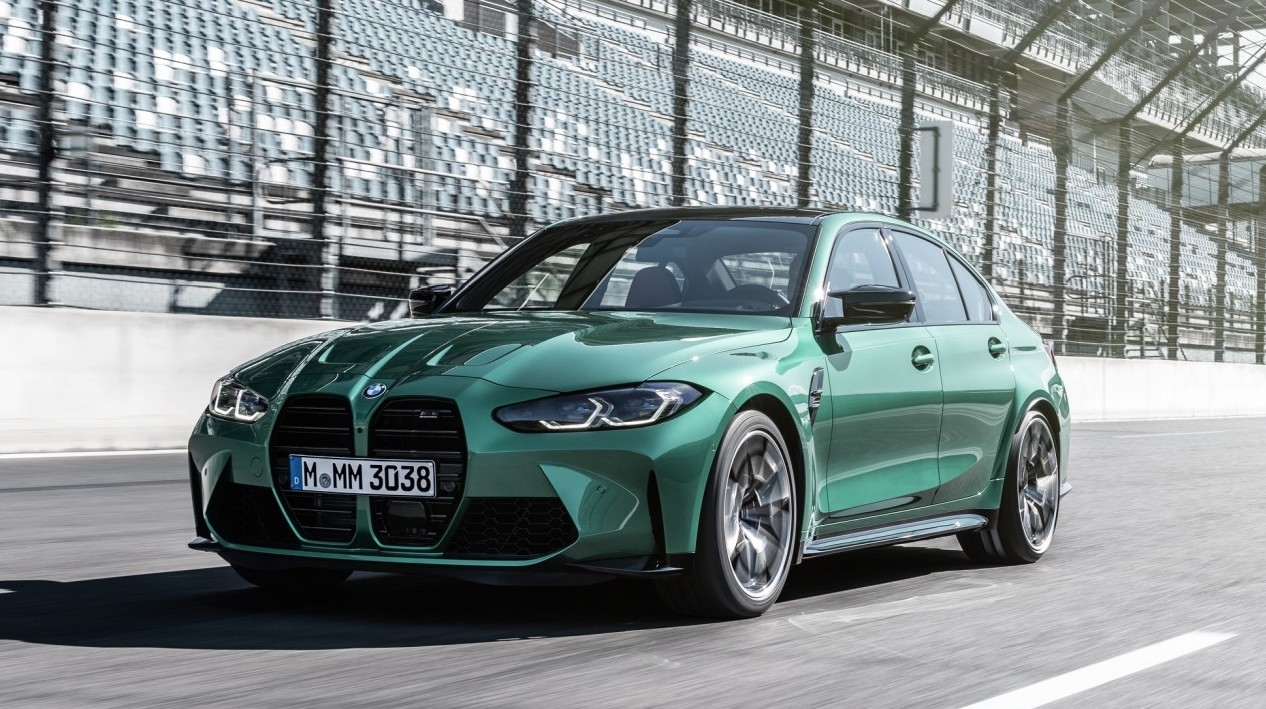
\includegraphics[width=0.6\linewidth]{figure/00-g80} \end{center}
\item
  The Authority for Info-communications Technology Industry of Brunei Darussalam (AITI) conducted the Household ICT Survey in 2018 and reported that 95\% percent of individuals personally use the internet on a daily basis, a slight decrease from 97\% in the year 2016. Estimates are accurate within 2\% margin of error with 95\% confidence.

  \begin{center}
\includegraphics[width=0.6\linewidth]{figure/00-aiti} \end{center}
\end{enumerate}

Your immediate thought should be ``how can I trust these figures?''. In general, it's always good to approach life with a healthy dose of skepticism. We certainly don't want to be duped by people claiming to present a version of the truth, when in reality it is a skewed version of the truth (or worse yet, false). In data we trust! But only if we are mathematically-savvy\ldots{}

\hypertarget{population-vs-sample}{%
\subsection*{Population vs sample}\label{population-vs-sample}}
\addcontentsline{toc}{subsection}{Population vs sample}

In both cases, the conclusion is drawn on a \emph{population} (i.e.~all of the subjects concerned) based on the information from a \emph{sample} (i.e.~a subset of the population).

\begin{enumerate}
\def\labelenumi{\arabic{enumi}.}
\item
  For BMW M Division, it is \textbf{impossible} to measure the entire population (obtain the acceleration rates), constituting \uline{all} BMW M3 (G80) cars that have been made and are yet to be made in the future. Often this is referred to as an \emph{infinite population} model.
\item
  For AITI, while possible, it is (economically) unfeasible to measure the entire population, i.e.~to ask everyone in Brunei whether or not they use the internet on a daily basis. It would be very difficult to knock on everybody's door and obtain responses in a timely manner (what if they're out of the country? what if they're sick? what if they just don't want to respond?). Anyone who has done any form of survey work will understand the intricate problems that might arise.
\end{enumerate}

In any case, it is important to make the distinction between population and sample.
The \emph{population} is defined to be the entire set of the objects concerned, and those objects are typically represented by some numbers. We \uline{do not know} the entire population in practice.
A \emph{sample} is a (randomly selected) subset of a population, and is a set of \uline{known data} in practice.

\begin{center}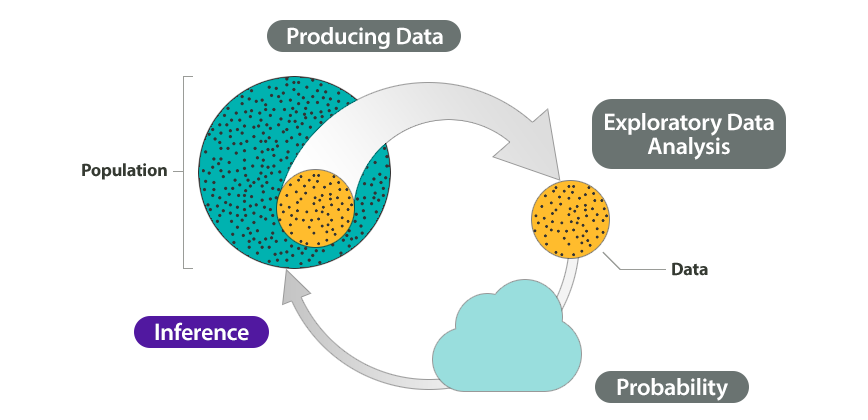
\includegraphics[width=0.9\linewidth]{figure/00-popsample} \end{center}

When people claim to have data (about some phenomenon), they typically imply that they have a \emph{sample} of the population, and not the population data itself. There are exceptions of course, for instance, a country's \emph{census} captures population data every 10 years. Another example is when the population itself is small such that all data can be collected easily.

A question that you might be thinking to yourself is the following:

\begin{quote}
Is doing analysis on the sample good enough? Will it reveal the same insights as if we're analysing the population data?
\end{quote}

The answer to this is that it depends on how you perform the sample! Things to look out for is definitely \emph{bias} in data collection methods. Here are some examples:

\begin{itemize}
\item
  Asking the question ``Can you live without the internet?'' via \textbf{an online poll} of adults. Think about it. How exactly can you ask people \emph{without} internet whether they can live without the internet? Clearly, the sample that you collect is biased towards those who are privileged enough to have access. And if you were wondering, yes this really \href{https://www.forbes.com/sites/niallmccarthy/2017/08/29/where-people-cant-live-without-the-internet-infographic/?sh=430d133643aa}{happened}.
\item
  Asking people to volunteer their responses typically lead to bias. It is suggested that those who has something to complain about will voice their opinions more than those who do not.
\item
  Other errors can crop up during data collection process which may skew the representation of the data (e.g.~duplicate data, missing data, substituted data, etc.)
\end{itemize}

It is certainly important that data be collected in a methodological manner, in order for valid inferences to be drawn.
Sampling methodology is beyond the scope of this course, however!

\hypertarget{parametric-models}{%
\subsection*{Parametric models}\label{parametric-models}}
\addcontentsline{toc}{subsection}{Parametric models}

For a given problem, it is quite advantagous to \textbf{assume} that a population obeys some \emph{probability distribution} law.
To be a little bit more concrete, suppose we assign the variable \(x\) to be the quantity of interest. Then we assume that the quantity of interest has a distribution function \(f(x|\theta)\) (we will recap the concept of distribution functions in the next chapter!).
Furthermore,

\begin{itemize}
\item
  The form of the distribution i.e.~\(f(\cdot|\theta)\) is known (e.g.~normal, Poisson, exponential, etc.).
\item
  The ``specifics'' of the distribution is (assumed to be) \textbf{not known}, but potentially knowable if data were available.
\end{itemize}

The unknown characteristics of the distribution are traditionally represented by \(\theta\) (such as the mean, variance, rate, etc.--any quantity that characterises how the distribution behaves).
We call \(\theta\) the \emph{parameter(s)} of the model.
Such an assumed distribution is called a \textbf{parametric model}.
For the two earlier examples,

\begin{enumerate}
\def\labelenumi{\arabic{enumi}.}
\item
  Let \(X =\) acceleration of BMW M3 G80 vehicles. Assume \(X\sim\N(\mu,\sigma^2)\). Here \(\btheta = (\mu,\sigma^2)^\top\), where \(\mu\) is the `true' acceleration rate. In this example, the parameter is 2-dimensional instead of unidimensional.
\item
  Let \(\{0,1\} \ni X =\) someone in Brunei uses the internet daily. Assume \(X\sim\Bern(p)\). Here \(\theta = p\), the `true' proportion of daily internet users in Brunei.
\end{enumerate}

There is no god-given right for your quantity of interest \(X\) to follow a particular distribution! These are simply assumptions, in order to make it easy to model reality. Parametric assumptions may be correct, or they may not. In fact, strictly speaking, \textbf{all models are wrong}, but some are useful (quote attributed to the British statistician George Box).

\begin{center}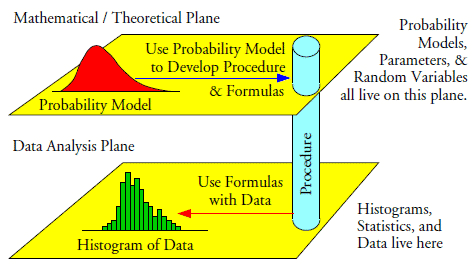
\includegraphics[width=0.8\linewidth]{figure/00-theoreticaldataplane} \end{center}

\hypertarget{a-sample-a-set-of-data-or-random-variablesa-duality}{%
\subsection*{A sample: a set of data or random variables?--A duality}\label{a-sample-a-set-of-data-or-random-variablesa-duality}}
\addcontentsline{toc}{subsection}{A sample: a set of data or random variables?--A duality}

A sample of size \(n\), \(\{X_1,\dots,X_n\}\), is also called a \emph{random} sample. It consists of \(n\) concrete numbers in a practical problem.
When I say `concrete' here, it means numbers that you can play around with--you can add them up, subtract them, plot them, take averages, and so on.
These would be numbers that you collect into a spreadsheet, say.

The more contentious part of the term `random sample' is the word `random' itself.
The word `random' encapsulates the possibility of the concrete numbers collected in the samples being different, by virtue of:

\begin{itemize}
\tightlist
\item
  The sample may be taken by different people or entities.
\item
  The sample may be obtained at a different time or location.
\item
  The sample may be measured using different instruments (albeit measuring the same thing).
\item
  etc.
\end{itemize}

Essentially, different samples may well be different subsets of a population.

With this, a sample may also be viewed as \(n\) (independent and identically distributed) random variables, simply because their values are conceptually not fixed (at least not until you observe them--but even then it is simply one possible realisation of potentially many others).

Now, if a sample is not random then perhaps there would be no need for statistics. But hardly ever would you find this to be the case.
Rigorous mathematical methods exist to deal with this randomness, and thus viewing samples as random variables allows us to assess the performance of a statistical method.

\hypertarget{variability-of-estimates}{%
\subsection*{Variability of estimates}\label{variability-of-estimates}}
\addcontentsline{toc}{subsection}{Variability of estimates}

Suppose you set out to answer questions 1 and 2 above by collecting some data.
This is what you find:

\hypertarget{bmw-m-example}{%
\paragraph*{\texorpdfstring{\uline{BMW M example}}{BMW M example}}\label{bmw-m-example}}
\addcontentsline{toc}{paragraph}{\uline{BMW M example}}

A sample of \(n=38\) gave the sample mean
\[\bar X_n = \frac{1}{n}\sum_{i=1}^n X_i = 3.9\]
In words, the average acceleration (0-100 km h-1) of the sample of cars yielded the value 3.9 seconds. But realise that a different sample may well give a different sample mean. For instance, 29 YouTubers and other social media ``influencers'' were given access to the new M3 on a race track, and their sample mean yielded \(\bar X_n = 3.4\).

What do we make of this discrepancy? Whose figure do we trust? It doesn't seem so satisfying to know that different samples will give different results. For instance, what do you tell the public or media about the acceleration figure of the new M3s? Evidently relying on a singular measure (in this case the mean) is not enough. Moreoever, it keeps on changing in value!

The key is to be able to employ \emph{probabilistic statements} about our results. For instance, ``\emph{the acceleration figure is 3.9 plus or minus 0.01 about 95\% of the time when we sample}'' is a much more confident statement to make, rather than providing a figure that keeps on changing.

By treating the data \(X_1,\dots,X_n\) as random variables, it is implied that \(\bar X_n\) is also a random variable. Everything that is random should have a distribution. If the distribution of
\(\bar X_n\) concentrates closely around the unknown \(\mu\), then it is a good estimator!

\hypertarget{aiti-example}{%
\paragraph*{\texorpdfstring{\uline{AITI example}}{AITI example}}\label{aiti-example}}
\addcontentsline{toc}{paragraph}{\uline{AITI example}}

For the AITI example, there is that statement \emph{`\ldots accurate to within 2\% margin of error with 95\% confidence'}. This statement alludes to the variability of the estimate, if another random sample was obtained.

\begin{itemize}
\item
  The estimate in this case was also the sample mean (proportion of people who use the internet on a daily basis),
  \[
  \hat p = \bar X_n = \frac{1}{n}\sum_{i=1}^n X_i.
  \]
\item
  Mathematically, the confidence statement reads
  \[
  \Pr(|\hat p - p| \leq 0.02 ) = \Pr\big(p\in [\hat p-0.02, \hat p + 0.02]\big) = 0.95
  \]
  that is, the true value is covered 95\% of the time inside an interval of width 0.02 under repeated sampling. This statement is made possible due to the \emph{randomness} of the estimator \(\hat p\).
\end{itemize}

\hypertarget{probability-and-statistics}{%
\section*{Probability and statistics}\label{probability-and-statistics}}
\addcontentsline{toc}{section}{Probability and statistics}

Thus far, we have thrown the term `inference' around and maybe we've all taken it for granted.
Cambridge's dictionary defines \emph{infer} as `to reach an opinion from available information or facts'.
And indeed that is what we are ultimately interested in when we analyse data.
Sure, there might be that random element to the data that we have to contend with, but it is about reaching some form of conclusion one way or another using data.
In the previous section, we've just implicitly described the three main activities concerning \uline{statistical inference}.

\begin{enumerate}
\def\labelenumi{\arabic{enumi}.}
\item
  \textbf{Point estimation}

  \emph{``What is \(\mu\)?''}
\item
  \textbf{Hypothesis testing}

  \emph{``Is \(\mu=3.4\) and not \(\mu=3.9\)?''}
\item
  \textbf{Interval estimation}

  \emph{``What's an upper and lower bound estimate for \(\mu\)?''}
\end{enumerate}

These three activities will be the main focus of this course, and we will formalise the notion of each one in turn.
Hopefully you can now appreciate how statistics is an inherently applied subject, making use of mathematics (probability in particular) to answer problems across a variety of fields.

What is the difference between probability and statistics? The following figure might be helpful.

\begin{center}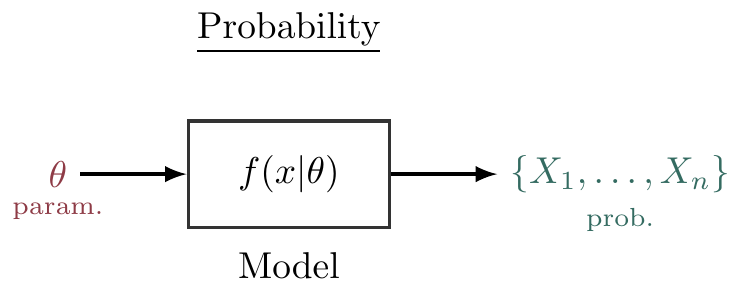
\includegraphics[width=0.48\linewidth]{bookdown-adv-stats_files/figure-latex/unnamed-chunk-1-1} \end{center}

\begin{center}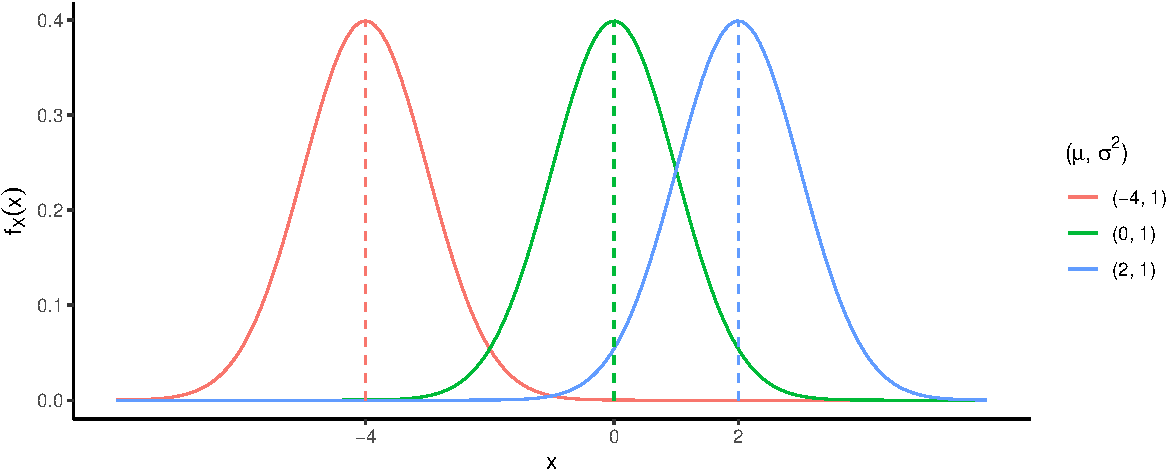
\includegraphics[width=0.48\linewidth]{bookdown-adv-stats_files/figure-latex/unnamed-chunk-2-1} \end{center}

Probability is a highly mathematical subject (although maybe the name doesn't seem to suggest it, it really has its origin in abstract measure theory). In probability, we ask questions like

\begin{itemize}
\tightlist
\item
  What is \(\E(X)\)? (expectations)
\item
  What is \(\Pr(X > a)\)? (probability calculations)
\end{itemize}

for some given value of \(\theta\) in an assumed family of parametric distributions.
Whereas in statistics, we are more interested in questions like

\begin{itemize}
\tightlist
\item
  What is \(\theta\)?
\item
  Is \(\theta\) larger than \(\theta_0\)?
\item
  How confident am I that \(\theta \in (\theta_l,\theta_u)\)?
\end{itemize}

given some observed data. I like to think of the two as reverse processes.

\begin{center}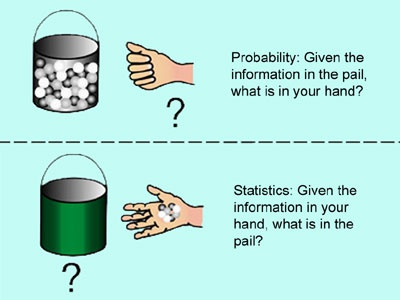
\includegraphics[width=0.8\linewidth]{figure/00-probstats} \end{center}

Statistics definitely needs probability for sure, so we will have to master probability theory before doing any statistical inference. On to the next chapter!

\hypertarget{part-prepare}{%
\part{Prepare}\label{part-prepare}}

\hypertarget{probability-theory-primer}{%
\chapter{Probability theory primer}\label{probability-theory-primer}}

As I was looking for a rationale as to why we begin statistical inference with learning about probability theory, I notice that C\&B couldn't have put it better:

\begin{quote}
The subject of probability theory is the foundation upon which all statistics is built, providing a means for modeling populations, experiments, or almost anouthing else that could be considered a random phenomenon. Through these models, statisticians are able to draw inferences about populations, inferences based on examination of only a part of the whole. --- George Casella \& Roger L. Berger in Statistical Inference
\end{quote}

By right, probability theory and the mathematics of random events deserves one dedicate module of its own. For our purposes, it suffices to `skim through the surface' as it were, and cover the basic and necessary ideas to move forward with statistical inference.

\hypertarget{learning-objectives}{%
\subsection*{Learning objectives}\label{learning-objectives}}
\addcontentsline{toc}{subsection}{Learning objectives}

By the end of this chapter, you will be able to:

\begin{itemize}
\tightlist
\item
  Compute probabilities of events by simple counting and application of various known probability results
\item
  Understand the notion of conditional and independent events, leading up to the application of Bayes' Theorem
\item
  Formalise mathematically the notion of random variables and make calculations using its distribution function
\item
  Compute expectations (and variances) including via the method of moment generating functions
\end{itemize}

\hypertarget{readings}{%
\subsection*{Readings}\label{readings}}
\addcontentsline{toc}{subsection}{Readings}

\begin{itemize}
\tightlist
\item
  Casella and Berger (2002)

  \begin{itemize}
  \tightlist
  \item
    All of Chapter 1 (skip sections 1.2.3 and 1.2.4).
  \item
    Chapter 2, section 2.2 and 2.3 only.
  \item
    Chapter 4, section 4.1, 4.2 and 4.5 only.
  \end{itemize}
\item
  Wasserman (2004)

  \begin{itemize}
  \tightlist
  \item
    All of Chapter 1.
  \item
    Chapter 2, sections 2.1--2.2, 2.5--2.8.
  \item
    Chapter 3, sections 3.1--3.5.
  \end{itemize}
\item
  Topics not covered: Counting and enumerating outcomes, moment generating functions (to be covered in the next topic), transformations of r.v., multivariate distributions (bivariate only).
\item
  \href{https://www.youtube.com/watch?v=lG4VkPoG3ko}{YouTube video: The medical test paradox}
\item
  \href{https://www.youtube.com/watch?v=HZGCoVF3YvM}{YouTube video: Bayes theorem}
\end{itemize}

\hypertarget{elementary-set-theory}{%
\section{Elementary set theory}\label{elementary-set-theory}}

A discussion of probability theory is almost always begun by talking about the concept of `sets'.
As the term implies, sets are a collection of things.
You're sure to come across sets before, such as the set of family members in your household, or the set of all natural numbers, or something even more funky like the set of all sets (the universal set\footnote{Which, as it turns out, is a paradox: \url{https://en.wikipedia.org/wiki/Russell\%27s_paradox}}).

When statisticians talk about sets it is usually in the context of conducting an ``experiment''\footnote{Although, we don't really mean it like how scientists mean experiments to be (we're not fiddling around with buttons or chemicals). I suppose it's more about the process of the (random) data generating mechanism itself.}.
The important bits are:

\begin{itemize}
\tightlist
\item
  The sample space \(\Omega\) is the set of possible outcomes of an experiment.
\item
  Elements \(\omega \in \Omega\) are called sample outcomes or realisations.
\item
  Subsets of \(E \subseteq \Omega\) are called events.
\end{itemize}

So whatever the context of the random process might be, we should be comfortable identifying what the sample space is, what its elements are, and what possible events might occur.

\begin{example}
In tossing a two-sided coin \(n \geq 2\) times, let \(H\) denote `heads', while \(T\) denote `tails'.
Let \(\bomega = (\omega_1,\dots,\omega_n)\) be the results of these coin tosses.
Then the sample space is \[
\Omega = \Big\{ \bomega \, \big|\, \omega_i \in \{H,T\} \Big\}.
\]
Let \(E\) be the event that the first head appears on the second toss. Then this event can be mathematically described as
\[
E = \Big\{ \bomega \, \big|\, \omega_1 = T, \omega_2 = H, \omega_i \in \{H,T\} \text{ for } i > 2 \Big\}.
\]
\end{example}

\hypertarget{set-operations}{%
\subsection{Set operations}\label{set-operations}}

There are several things that we can do to sets much like we can do to numbers in arithmetic. Here is an abridged version of set operations.

\begin{itemize}
\item
  The \textbf{complement} of an event \(A\), written \(A^c\), is the set of all elements that are not in \(A\): \(A^c = \{\omega \mid \omega\not\in A \}\).
\item
  The complement of \(\Omega\) is the empty set \(\emptyset = \{\}\).
\item
  The \textbf{union} of events \(A\) and \(B\) (thought of as ``A or B or both'') is defined
  \[
  A \cup B = \{\omega \in \Omega \,|\, \omega \in A \text{ or } \omega \in B \}.
  \]
\item
  The \textbf{intersection} of events \(A\) and \(B\) (thought of as ``A \emph{and} B'') is defined
  \[
  A \cap B = \{\omega \in \Omega \,|\, \omega \in A \text{ and } \omega \in B \}.
  \]
\item
  Unions and intersections on sets are \textbf{commutative}, \textbf{associative}, and \textbf{distributive}\footnote{See C\&B Thm 1.14}.

  \begin{itemize}
  \item
    Commutativity: \(A \cup B = B \cup A\) and \(A \cap B = B \cap A\).
  \item
    Associativity: \(A \cup (B \cup C) = (A \cup B) \cup C\) and \(A \cap (B \cap C) = (A \cap B) \cap C\).
  \item
    Disributive laws: \(A \cap (B \cup C) = (A \cap B) \cup (A \cap C)\) and \(A \cup (B \cap C) = (A \cup B) \cap (A \cup C)\).
  \end{itemize}
\item
  DeMorgan's Laws: \((A \cup B)^c = A^c \cap B^c\) and \((A \cap B)^c = A^c \cup B^c\)
\end{itemize}

It's pretty straightforward to prove the commutative, associative, distributive and DeMorgan's properties using the rules that precede them in the list. You may like to try this out yourself. Or you may have come across a kind of ``sketch proof'' involving \textbf{Venn diagrams}.

The operations of unions and intersections can be extended to infinite collections of sets as well.
If \(A_1,A_2,A_3,\dots\) is collection of sets, all defined on a sample space \(\Omega\), then
\begin{gather*}
\bigcup_{i=1}^\infty A_i = \{x \in \Omega \,|\, x\in A_i \text{ for some } i \}, \\
\bigcap_{i=1}^\infty A_i = \{x \in \Omega \,|\, x\in A_i \text{ for all } i \}.
\end{gather*}

\begin{example}
Let \(\Omega=(0,1]\) and define \(A_i=[1/i, 1]\). Then,
\begin{align*}
\bigcup_{i=1}^\infty A_i
&= \{1\} \cup [1/2, 1] \cup [1/3, 1] \cup \cdots = (0,1], \\
\bigcap_{i=1}^\infty A_i
&= \{1\} \cap [1/2, 1] \cap [1/3, 1] \cap \cdots = \{1\}.
\end{align*}
\end{example}

\hypertarget{partitions}{%
\subsection{Partitions}\label{partitions}}

We say that two events \(A\) and \(B\) are \textbf{disjoint} or \textbf{mutually exclusive} if \(A \cap B = \{ \}\). Disjoint sets have no points in common.
Suppose that \(A_1,A_2,\dots\) are events defined on \(\Omega\) such that they are (pairwise) disjoint, i.e.~
\[
A_i \cap A_j = \{ \}, \text{ for } i \neq j.
\]
Then the collection \(A_1,A_2,\dots\) forms a \textbf{partition} of \(\Omega\).
Partitions divide the sample space into non-overlapping pieces.

\begin{example}
A deck of playing cards has four suits: \(\clubsuit, \diamondsuit, \spadesuit, \heartsuit\). Let \(A=\{\clubsuit,\diamondsuit\}\) and \(B=\{\spadesuit, \heartsuit\}\). Then \(A\) and \(B\) form a partition of the sample space.
\end{example}

\begin{example}
The set \(\{\bbR_+, \bbR_{-}, \{0\}\}\) (ie the set of positive reals, negative reals, and zero respectively) is a partition of the real numbers \(\bbR\) since

\begin{itemize}
\tightlist
\item
  \(\bbR_{+} \cup \bbR_{-} \cup \{0\}=\bbR\);
\item
  \(\bbR_{+} \cap \bbR_{-} = \bbR_{+} \cap \{0\} = \bbR_{-} \cap \{0\} = \{ \}\); and
\item
  \(\{\bbR_{+}\), \(\bbR_{-}\), and \(\{0\}\}\) are all non empty.
\end{itemize}

Note that \(\{0\}\) is not an empty set. It contains exactly one element, the number zero.
\end{example}

\hypertarget{axiomatic-probability}{%
\section{Axiomatic probability}\label{axiomatic-probability}}

In principle, we can understand and easily grasp the notion of probability as the ``frequency of an event occurring''.
But how do we operationalise this concept? That is, by what rules and mechanisms are we allowed to assign probabilities to events?
If we can overcome this task and are able to assign probabilities to (random) events in an experiment, then we can start to analyse them statistically!

\hypertarget{probability-as-a-measure}{%
\subsection{Probability as a measure}\label{probability-as-a-measure}}

Let us take a measure-theoretic approach to defining probabilities.
We will dive straight into the rigors of definitions before providing a somewhat apologetic rationale as to why such mathematical difficulties are required for probability theory.

As the name implies, measure theory is the theory about how we measure things (duh!).
Measure itself is a fundamental concept in mathematics, and it would be useful to come up with a mathematical framework for how we deal with everyday concepts like length, mass, area, volume, and so on.
Importantly, such a framework allow us to reliably measure in even higher dimensions or onto more abstract constructs not yet imaginable.

Intuitively, a measure is simply a function whose input is the thing we want to measure (let's call it a set), and whose output is a non-negative number.
Don't worry, a formal definition will follow, but for now, call this function \(\mu\).
It would be fair to expect a measure \(\mu\) to satisfy

\begin{itemize}
\tightlist
\item
  \(A \subseteq B \Rightarrow \mu(A) \leq \mu(B)\)
\item
  \(A \subseteq B \Rightarrow \mu(B-A)= \mu(B) - \mu(A)\)
\item
  If \(\{A_1,A_2,\dots\}\) are mutually exclusive sets (disjoint), then \(\mu\left(\cup_{i=1}^\infty A_i \right) = \sum_{i=1}^\infty \mu(A_i)\)
\end{itemize}

The first property simply says that if \(A\) is a subset of \(B\), then the measure of \(A\) is at most the measure of \(B\).
The second property follows this up by saying that the measure of the set \(B-A\), that is, the set that is obtained by starting with \(B\) and taking away the parts that is contained in \(A\), then the measure of this created set is the difference between the measures of \(B\) and \(A\).
Finally, the third property, also known as \emph{countable additivity}, simply states that the measure of the whole is equal to the sum of the parts.
It turns out that the first and second properties follow from the third (and the fact that a measure cannot be negative)--see Definition \ref{def:measure}.

So we have this intuition about what the measure should be, but what about the stuff we want to measure?
For our purposes, we are interested in measuring subsets of \(\Omega\).
We ask, are we able to measure all possible subsets of \(\Omega\)?
At a glance, perhaps if \(\Omega\) is countable (e.g.~\(\Omega=\{1,2,3\}\)), it is easy to describe the subsets of \(\Omega\) through the power set\footnote{For the example at hand, the power set is \(\cP(\Omega)=\{ \{\}, \{1\}, \{2\}, \{3\}, \{1,2\}, \{1,3\}, \{2,3\}, \{1,2,3\} \}\)} \(\cP(\Omega)\), which is the set of all possible subsets of \(\Omega\), but what about when \(\Omega\) is uncountable (e.g.~an interval \(\Omega=[0,1]\in\bbR\)).
Given a sample space \(\Omega\), we need to define the largest possible collection of subsets of \(\Omega\) that can be observed and on which we can assign valid measure.

\begin{definition}[\(\sigma\)-algebra]
\protect\hypertarget{def:sigmaalgebra}{}\label{def:sigmaalgebra}

A collection \(\cF\) of subsets of a set \(\Omega\) is called a \textbf{\(\sigma\)-algebra} if it satisfies the following conditions:

\begin{enumerate}
\def\labelenumi{\roman{enumi}.}
\tightlist
\item
  If \(A \in \cF\), then \(A^c \in cF\) \emph{{[}closed under complementation{]}}.
\item
  If \(A_1,A_2,\cdots \in \cF\), then \(\cup_{i=1}^\infty A_i \in \cF\) \emph{{[}closed under countable unions{]}}.
\item
  \(\{\} \in \cF\) \emph{{[}contains the empty set{]}}.
\end{enumerate}

\end{definition}

As a remark, condition iii. can be replaced with \(\Omega\in\cF\) by virtue of condition i..
The \(\sigma\)-algebra is a collection of events or subsets of the sample space \(\Omega\), including \(\Omega\) itself and the empty set \(\{\}\), which is closed under countable applications of set operations.
This is because DeMorgan's Law allows us to write the countable union property in iii. also as \emph{countable intersections}: If \(A_1,A_2,\cdots \in \cF\), then by i. \(A_1^c,A_2^c,\cdots \in \cF\), and hence \(\cup_{i=1}^\infty A_i\in\cF\) and also its complement. By DeMorgan's Law,
\[
\left( \cup_{i=1}^\infty A_i^c \right)^c = \cap_{i=1}^\infty A_i.
\]

Sets contained in \(\cF\) are called \textbf{measurable sets}.

The \(\sigma\)-algebra is an important condition for measure to not breakdown, because it helps draw a line as to which subsets of the sample space is measurable, and which is not.
Out of interest, condition iii. in Definition \ref{def:sigmaalgebra} is the condition that makes \(\cF\) a \(\sigma\)-algebra (the \(\sigma\) stands for countable \uline{\textbf{s}}um).
Without this condition, one ends up with just an \emph{algebra} of sets, one that is most likely \emph{too small}, failing to contain sets that we would like assign a measure.

Let's take a look at some examples of \(\sigma\)-algebras.

\begin{example}

\begin{enumerate}
\def\labelenumi{\arabic{enumi}.}
\item
  The trivial \(\sigma\)-algebra: \[\big\{ \{\}, \Omega \big\}.\] This corresponds the case of no information.
\item
  The power set of the sample space \(\Omega\): \[\big\{ A \mid A \subseteq \Omega \big\}.\] This corresponds the case of full information.
\item
  The collection \(\big\{ \{\}, A, A^c, \Omega \big\}\) is a \(\sigma\)-algebra, for any \(A\subseteq \Omega\).
\item
  Let \(\Omega = \{a,b,c,d\}\). A possible\footnote{You may notice that other \(\sigma\)-algebras are indeed possible, e.g.~the power set of \(\Omega\) in this case. There is a notion of the \emph{smallest} \(\sigma\)-algebra containing the collection of ``basic events''. Luckily for us, the event space that we will usually be working with will be the smallest \(\sigma\)-algebra without much technicalities, so we shall not explore this concept any further.} \(\sigma\)-algebra is \[\big\{\{\}, \{a,b,c,d\}, \{a,b\}, \{c,d\} \big\}.\]
\item
  Define \(B(s)\) to be a square of side length \(s\). Let \(\Omega\) be the collection of points in \((0,1)\times(0,1)\subset \bbR^2\) contained within the a unit square \(B(1)\). Then \[\cF=\{ \text{Collection of points contained in the square } B(s) \text{ with } s \in (0,1) \}.\] It should be clear there are uncountably many such squares that can be fit within the unit square.
\end{enumerate}

\end{example}

Just as a remark, most introduction to probability measure will deal with finite or countable sets when introducing \(\sigma\)-algebras, giving readers an impression that it's only possible to define \(\sigma\)-algebras on such sets. The fifth example above gives an example of a \(\sigma\)-algebra which is uncountable.

The twin \((\Omega,\cF)\) is called a \emph{measurable space}. This sort of defines the ``parts'' of our problem which are measurable, as per Definition \ref{def:sigmaalgebra}. What's missing is a measure, i.e.~the thing that actually tells us `how long a piece of string is', so to speak\footnote{\url{https://idioms.thefreedictionary.com/How+long+is+a+piece+of+string\%3F}}. We now define a measure as follows.

\begin{definition}[Measure]
\protect\hypertarget{def:measure}{}\label{def:measure}

A \emph{measure} \(\mu\) is a non-negative real valued function defined on a \(\sigma\)-algebra, i.e.~\(\mu:\cF\to\bbR_{\geq 0}\cup\{\infty\}\), where \(\bbR_{\geq 0}\) are the non-negative real numbers and \(\cF\) a \(\sigma\)-algebra of subsets of \(\Omega\). The measure \(\mu\) satisfies the following properties:

\begin{enumerate}
\def\labelenumi{\roman{enumi}.}
\tightlist
\item
  \(\mu(\{\})=0\).
\item
  \(\mu\) is countably additive, i.e.~if \(A_1,A_2,\dots\) are disjoint events, then \[\mu\left( \cup_{i=1}^\infty A_i \right) = \sum_{i=1}^\infty \mu(A_i).\]
\end{enumerate}

\end{definition}

If, in addition the measure of the entire sample space is normalised (i.e.~\(\mu(\Omega)=1\)), then \(\mu\) is called a \textbf{probability measure}. We will see this in the next section.

The triplet \((\Omega,\cF,\mu)\) is called a \emph{measure space} (note that without the measure it is called a measurable space).
This space simply tells us the parts needed for well-defined measure to take place on the subsets of \(\Omega\).

\begin{example}

\begin{enumerate}
\def\labelenumi{\arabic{enumi}.}
\item
  The counting measure. Let \(\Omega\) be a countable set {[}You may be creative as you like here to make this less abstract, e.g.~the books on your shelf or the members of your family, although the set need not be finite{]}. Let \(\cF=\cP(\Omega)\) be the power set of \(\Omega\). For all sets \(A\in\cA\), define \[\mu(A) = \begin{cases} |A| & A \text{ has finitely many elements}\\ \infty &\text{otherwise} \end{cases}\] where the operator \(|\cdot|\) represents the \emph{cardinality} of the set, i.e.~the number of elements it contains (its size).
\item
  The Lebesgue measure in one dimension. Let \(\Omega=\bbR\), and define \(\cF\) to contain all sets of the form

  \begin{itemize}
  \tightlist
  \item
    {[}a,b{]}, i.e.~closed intervals,
  \item
    (a,b), i.e.~open intervals,
  \item
    (a,b{]}, i.e.~open-closed intervals; and
  \item
    {[}a,b), i.e.~closed-open intervals.
  \end{itemize}

  for all real numbers \(a\) and \(b\). We can deduce that the \(\sigma\)-algebra \(\cF\) contains all possible ``nice'' intervals of the real line, including unbounded intervals and even singletons, which means any continuous partition of the real line can be measured (including a point, which should have measure zero). To see this, using the properties of \(\sigma\)-algebras,

  \begin{itemize}
  \item
    unbounded intervals are in \(\cF\), since, for instance \[(x,+\infty)=\cup_{i=1}^\infty(x,x+i).\]
  \item
    singletons are in \(\cF\), since \[\{x\}=\cap_{i=1}^\infty (x-1/i,x+1/i).\]
  \end{itemize}

  This set \(\cF\) has a special name, called the Borel \(\sigma\)-algebra.

  All that's left is to define the measure. The Lebesgue measure \(\mu\) assigns the usual concept of length to any continuous interval on \(\bbR\) (to be precise, the Borel \(\sigma\)-algebra on \(\bbR\)): \[\mu\left(A\right)=b-a\]
  where \(A\) is any interval of \(\bbR\) of the above forms (closed, open, open-closed, closed-open). This measure works even for singleton sets or unbounded intervals.
\end{enumerate}

\end{example}

\hypertarget{axioms-of-probability}{%
\subsection{Axioms of probability}\label{axioms-of-probability}}

In the previous section, we defined a measure space as the triplet \((\Omega,\cF,\mu)\).
This formulation lets us work on the set of interest \(\Omega\), and defines the possible measurable subsets \(\cF\subseteq \Omega\), as well as the measuring device \(\mu\).
This framework generalises the intutive notions of length, area, and volume to higher dimensions and more abstract notions.

In probability theory, we are interested in making use of measure theory to assign probabilities to events. So again in the context of conducting an ``experiment'',

\begin{itemize}
\tightlist
\item
  The sample space \(\Omega\) is the set of possible outcomes \(\{\omega_1,\omega_2,\dots\}\) of the experiment.
\item
  The \(\sigma\)-algebra \(\cF\subseteq\Omega\) would define the set of possible outcomes that are measurable, and are able to be assigned probabilities. \(\cF\) is known as the \emph{event space}.
\end{itemize}

All that's left is to define a \emph{probability measure} on the measurable space \((\Omega,\cF)\).

\begin{definition}[Axioms of Probability]
Given a measurable space \((\Omega,\cF)\), a \emph{probability measure} (or \emph{probability function}) is a function \(\bbP:\cF\to[0,1]\) that satisfies the following three conditions:

\begin{enumerate}
\def\labelenumi{\roman{enumi}.}
\tightlist
\item
  \(\bbP(E) \geq 0, \forall E \in \cF\).
\item
  \(\bbP(\Omega) = 1\).
\item
  For pairwise disjoint events \(A_1,A_2,\dots\), \[\bbP\bigg( \bigcup_{i=1}^\infty A_i  \bigg) = \sum_{i=1}^\infty A_i.\]
\end{enumerate}

These three conditions are commonly known as the \emph{Axioms of Probability}, or \emph{Kolmogorov Axioms}.
\end{definition}

This is pretty much similar to the definition of the measure \(\mu\) for a measure space, except for the unitarity requirement \(\bbP(\Omega)=1\).
The first and second condition implicitly states that probabilities are always \uline{finite}, by the results of Theorem \ref{thm:derivedprobres1} below.
In contrast, measure theory allows for infinite measure.

The second condition above states that the probability of \emph{at least} one of the elementary events in the entire space will definitely occur.
One common misunderstanding here is to read the statement as ``the probability of all of possible events occurring is 1'', which is a rarer thing in most situations.

As a remark, the above axioms does not tell us anything about what the functional form of \(\bbP\) actually is.
It is pretty abstract, but the good thing is that any such function that satisfies the above three axioms is by definition a probability function.
At this point, there is still no notion of \emph{randomness} in play.
All we are doing is providing the building blocks to be able to assign a numerical representation of (un)certainty of some particular event happening.

\begin{figure}

{\centering 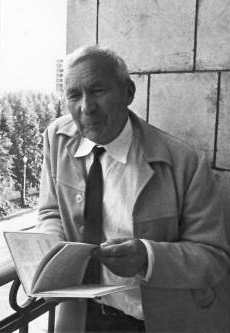
\includegraphics[width=0.5\linewidth]{figure/kolmogorov} 

}

\caption{Andrey Nikolaevich Kolmogorov 25 April 1903--20 October 1987. Widely considered to be the father of probability theory.}\label{fig:kolmogorov}
\end{figure}

As mentioned, any function abstract or concrete satisfying the Probability Axioms is regarded as a probability function.
But what does the probability number represent, and what does it actually mean?
Broadly speaking, there are two main interpretation of probabilities.

\begin{enumerate}
\def\labelenumi{\arabic{enumi}.}
\item
  The \textbf{frequentist} interpretation is one that relies on ``long run'' frequencies. A probability of heads being 50\% in a coin flip is interpreted to mean the following: If we flip the coin many times, then the proportion of heads that is observed will be 50\% in the long run.
\item
  The \textbf{subjectivist} or Bayesian interpretation is that the probability measures an observer's strength of belief that the event is true. Put a different way, it is the measure of ignorance on the observers part on what has happened. When a coin is flipped, it has landed either heads or tails, and this much is certain. What is uncertain is my \emph{knowledge about the coin}, rather than the outcome of the coin itself. Setting a 50\% probability for heads occuring implies that I am willing to bet at a 1:1 odds that the coin landed heads.
\end{enumerate}

\begin{example}[C\&B 1.2.5]
Consider the simple experiment of tossing a coin.
Define the sample space to be \(\Omega=\{H,T\}\), as representing the only two possible outcomes \(H=\) heads or \(T=\) tails.

What is the probability of heads occurring?
The Axioms of Probability does not help us in this regard! (I mean, it does not give us a functional form for the probabilities)

Perhaps a function that assigns equal probability to either event would be a good place to start, so we require
\begin{equation}
\bbP(\{H\})=\bbP(\{T\}). \label{eq:headtail1}  
\end{equation}
At this point, we still don't know their values--the probabilities could be 0.1, 0.2, 0.3, or any other value.
Or could they?

Since \(\Omega = \{H\} \cup \{T\}\), we know that by the Probability Axioms that
\begin{align}
1 = \bbP(\Omega) 
&= \bbP\left( \{H\} \cup \{T\} \right) \nonumber \\
&= \bbP(\{H\}) + \bbP(\{T\}) \label{eq:headtail2}
\end{align}
so the only possible value that satisfies both \eqref{eq:headtail1} and \eqref{eq:headtail2} is
\[
\bbP(\{H\})=\bbP(\{T\}) = 0.5.
\]
\end{example}

Of course, without the restriction of equal probability in \eqref{eq:headtail1}, then any two numbers satisfying \eqref{eq:headtail2} and the Probability Axioms would be valid, e.g.~\(\bbP(\{H\})= 0.8\) and \(\bbP(\{T\}) = 0.2.\)

\begin{example}
Two six-sided dice are thrown and the outcome for both dice are recorded.

\begin{itemize}
\item
  As there are 36 possible outcomes, the sample space is
  \[
  \Omega = \big\{ \omega_{ij}=\{i,j\} \mid i,j =1,\dots,6 \big\}
  \]
\item
  Suppose we are interested in the event \(E\) defined to be \emph{`the sum of the two scores is 6'}. These would be the events
  \[
  E := \big\{ \{1,5\}, \{2,4\}, \{3,3\}, \{4,2\}, \{5,1\} \big\}.
  \]
  One may easily construct a \(\sigma\)-algebra \(\cF\) (for example, the power set of \(\Omega\)) and verify that the event \(E\) is contained within it. So this is a measurable event.
\end{itemize}

So at this point, we might be thinking about a suitable probability function so that we may assign a probability to the event \(E\).
Especially if the two dice are fair, it seems reasonable to assume that any of the outcome in \(\omega_{ij}\in\Omega\) is equally likely to occur, so we set \(\bbP(\omega_{ij}) = 1/36\) for any \(i,j =1,\dots,6\).
In particular, the probability of any event should be proportional to the total number of outcomes in \(\Omega\).
As a quick exercise, you may check that such a probability function satisfies all the Kolmogorov Axioms.

\begin{align*}
\bbP(E) &= 
\bbP\left( \{1,5\} \cup \{2,4\} \cup \{3,3\} \cup \{4,2\} \cup \{5,1\} \right) \\
&= \bbP( \{1,5\}) + \bbP(\{2,4\}) + \bbP(\{3,3\}) \\
& \hspace{1em} + \bbP(\{4,2\}) + \bbP(\{5,1\}) \\
&= \frac{5}{36}
\end{align*}

Alternatively, we could have also easily argued that
\[
\bbP(E) = \frac{|E|}{|\Omega|} = \frac{5}{36}.
\]
\end{example}

As a remark, it would be very cumbersome to have to check the Kolmogorov Axioms every time we encounter a probability function.
For problems like the above, we won't run into any technical issues because the sample space is finite and/or countable\footnote{See Theorem 1.2.6 in C\&B.}.
In general, most of the problems we will come across will satisfy the axioms automatically, especially with ``nice'' sample space and events, so we usually don't check axioms all the time.

At this point, most textbooks go into a section about \emph{counting}, namely using methods like combinations and permutations.
I'm sure you've encountered this previously in your statistics classes, and appreciate how useful they are when trying to calculate probabilities as being ``the number of outcomes in the event space'' divided by ``the number of outcomes in the sample space''.
However, our focus for this course is to get to the inference section, and the topic of counting does not contribute much to that understanding, so I shall skip it.

\hypertarget{derived-probability-results}{%
\subsection{Derived probability results}\label{derived-probability-results}}

Let us now look at some useful probability results that can be derived from the probability axioms.

\begin{theorem}
\protect\hypertarget{thm:derivedprobres1}{}\label{thm:derivedprobres1}

Let \((\Omega,\cF,\bbP)\) be a probability space. For any \(E\in\cF\),

\begin{enumerate}
\def\labelenumi{\roman{enumi}.}
\tightlist
\item
  \(\bbP(\{\}) = 0\);
\item
  \(\bbP(E) \leq 1\); and
\item
  \(\bbP(E^c)=1-\bbP(E).\)
\end{enumerate}

\end{theorem}

An important thing that we learn here is that probabilities are always finite and bounded within \([0,1]\), i.e.~for any event \(E\), \(0 \leq \bbP(E) \leq 1\).
So please, do not make the mistake of reporting \emph{negative probabilities} or probabilities greater than one--they are mathematically impossible\footnote{At least within the framework of the Kolmogorov Axioms. See: \url{https://en.wikipedia.org/wiki/Negative_probability}}!

The proof of Theorem \ref{thm:derivedprobres1} is left an exercise. Try this out for yourself!

Further results regarding two events in the sample space based on the Probability Axioms:

\begin{theorem}

Let \((\Omega,\cF,\bbP)\) be a probability space. For any \(A,B \in\cF\),

\begin{enumerate}
\def\labelenumi{\roman{enumi}.}
\tightlist
\item
  \(\bbP(B \cap A^c) = \bbP(B) - \bbP(A\cap B)\);
\item
  \(\bbP(A \cup B) = \bbP(A) + \bbP(B) - \bbP(A \cap B)\); and
\item
  If \(A \subseteq B\), then \(\bbP(A) \leq \bbP(B)\).
\end{enumerate}

\end{theorem}

While these results are not so self-evident from the Probability Axioms, it may be useful to employ Venn diagrams to visualise the above statements.

\begin{center}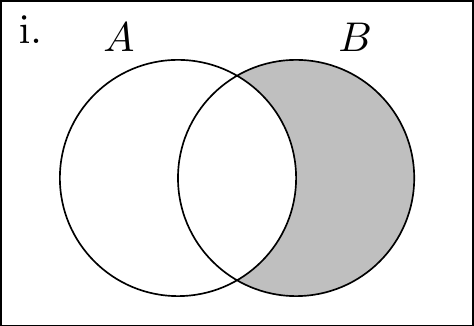
\includegraphics[width=0.32\linewidth]{bookdown-adv-stats_files/figure-latex/venn1-1} \end{center}

\begin{center}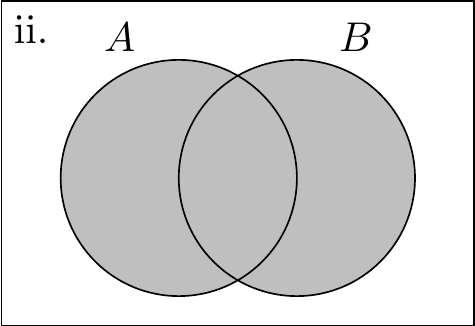
\includegraphics[width=0.32\linewidth]{bookdown-adv-stats_files/figure-latex/venn2-1} \end{center}

\begin{center}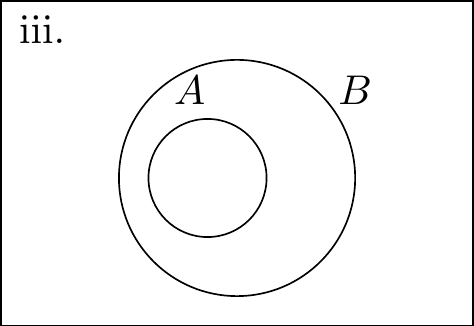
\includegraphics[width=0.32\linewidth]{bookdown-adv-stats_files/figure-latex/venn3-1} \end{center}

\begin{proof}

\begin{enumerate}
\def\labelenumi{\roman{enumi}.}
\item
  Note that \(B\) is composed of the two disjoint sets \(B= \{B\cap A\} \cup \{ B \cap A^c\}\), so we have \[\bbP(B) = \bbP(B\cap A) + \bbP(B \cap A^c),\] and the desired results is obtained after rearranging.
\item
  Using the identity \[A \cup B = (A \cup B) \cap \overbrace{(A \cup A^c)}^\Omega=A \cup \{B \cap A^c \},\] we have that (since the two events are disjoint)
  \begin{align*}
  \bbP(A \cup B) &= \bbP(A) + \bbP(B \cap A^c) \\
  &= \bbP(A) + \bbP(B \cap A^c) \\
  &= \bbP(A) + \bbP(B) - \bbP(B\cap A).
  \end{align*}
\item
  Since \(A \subseteq B\), \(A \cap B = A\), using i. we get \[0 \leq \bbP(B \cap A^c) = \bbP(B) - \overbrace{\bbP(A\cap B)}^{\bbP(A)},\] thus obtaining the desired result.
\end{enumerate}

\end{proof}

\begin{theorem}[Law of Total Probability]
\protect\hypertarget{thm:lawoftotalprob}{}\label{thm:lawoftotalprob}Let \((\Omega,\cF,\bbP)\) be a probability space. Let \(A\in\cF\) and consider a (countably infinite) partition of the sample space \(C_1,C_2,\dots\) such that \(C_i\cap C_j = \{\}\) for any \(i,j\) and \(\bigcup_{i=1}^\infty C_i = \Omega\). Then
\[
\bbP(A) = \sum_{i=1}^\infty \bbP(A \cap C_i).
\]
\end{theorem}

We may visualise the partitions of the sample space \(C_i\) as well as the event \(A\) of interest as follows:

\begin{center}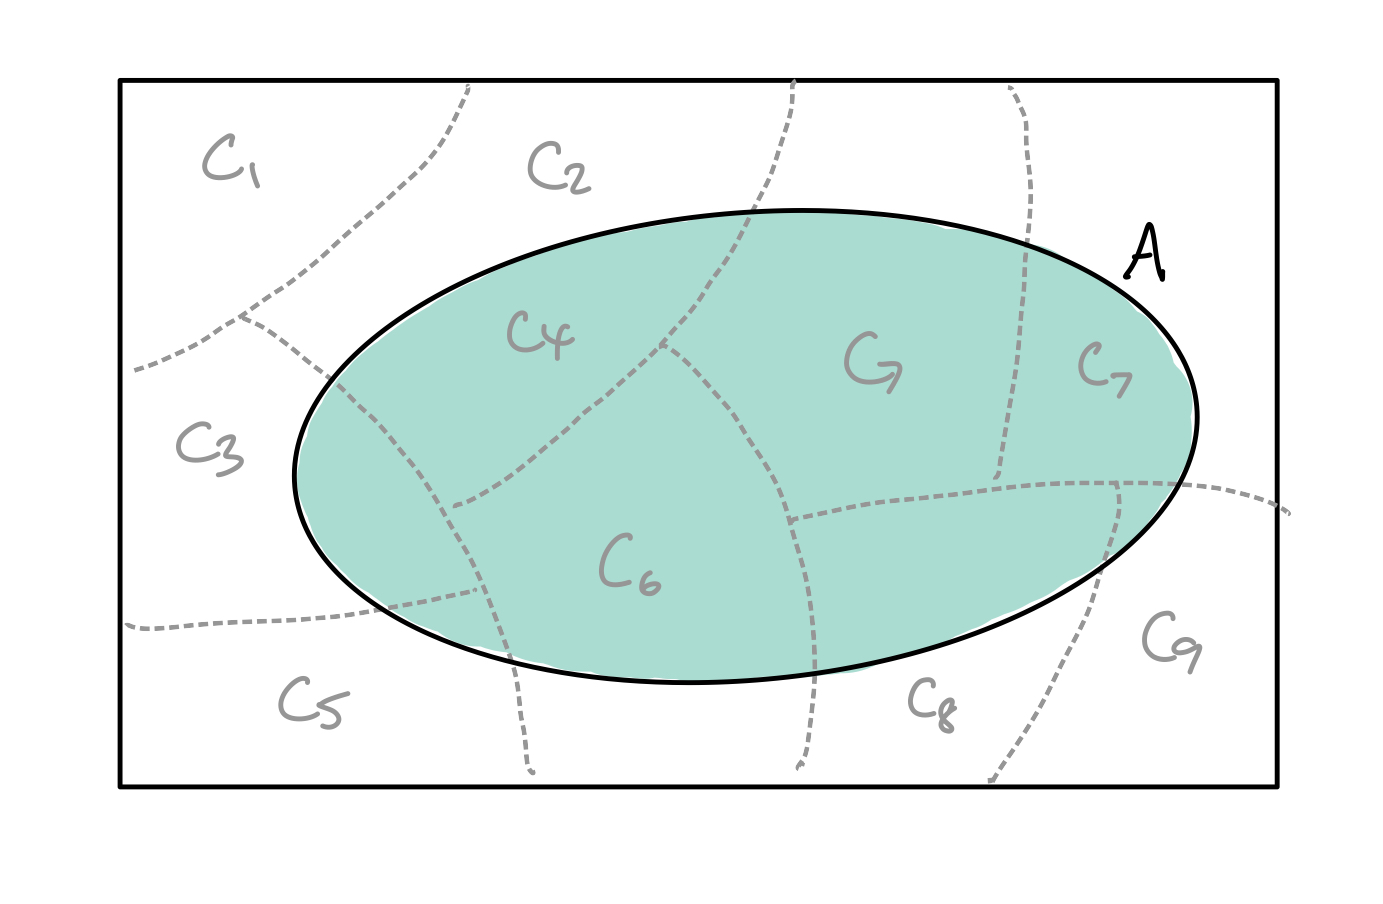
\includegraphics[width=0.8\linewidth]{figure/lawoftotalprob} \end{center}

Of course, we can only show a finite number of partitions for illustration, but this works for infinitely many countable partitions as well. We can see that the set \(A\) is simply made up of the intersections of \(A\) and the partitions.
Some of these intersections will be empty, but that's OK.

\begin{proof}
Write
\[
A = A \cap \Omega = A \cap \left(\bigcup_{i=1}^\infty C_i\right) = \bigcup_{i=1}^\infty(A \cap C_i)
\]
Evidently the events in the union on the right hand side of the equality are disjoint, since \(C_i\) themselves are disjoint.
Therefore,
\begin{align*}
\bbP(A) 
&= \bbP\left(\bigcup_{i=1}^\infty(A \cap C_i) \right) \\
&= \sum_{i=1}^\infty \bbP(A \cap C_i)
\end{align*}
as required.
\end{proof}

\hypertarget{why-measure-theory}{%
\subsection{Why measure theory?}\label{why-measure-theory}}

\emph{You may treat this section as optional, but it would deepen your understanding of probability theory.}

Consider the uniform distribution on a random variable \(X\) on the unit interval, denoted \(X\sim\Unif(0,1)\). You may have come across this before, and know that the probability that \(X\) lies in any interval contained in \([0,1]\) is simply the length of the interval, i.e.
\begin{equation}
\bbP\big([a,b]\big) = \bbP\big([a,b)\big) = \bbP\big((a,b]\big) = \bbP\big((a,b)\big) = b-a, \label{eq:meas1}
\end{equation}
for \(0 \leq a \leq b \leq 1\). This definition works fine for the degenerate case \(\bbP(\{a\})=0\) for the singleton set \(\{a|a\in(0,1)\}\).
In general, if \(A\) and \(B\) are disjoint subsets of \([0,1]\) then
\begin{equation}
\bbP(A \cup B) = \bbP(A) + \bbP(B),
\end{equation}
and we can even extend this notion to that of \emph{countable additivity}
\begin{equation}
\bbP\left( \cup_{i=1}^\infty A_i \right) = \sum_{i=1}^\infty \bbP(A_i), \label{eq:meas2}
\end{equation}
for disjoint sets \(\{A_1,A_2,\dots\}\)\footnote{A concrete example of this is for the sets \(A_1=(0,1/2)\), \(A_2=(1/2, 3/4)\), \(A_3=(3/4,7/8)\), and so on (adding half the interval at each iteration). One finds that the measure of the countable union is \(\sum_{i=1}^\infty (1/2)^i=1\).}.

For a uniform measure on \([0,1]\), one expects that the measure of some subset \(A \subseteq [0,1]\) to be unaffected by ``shifting'' (with wrap-around) of that subset by some fixed amount \(r\in[0,1]\).
Define the \emph{\(r\)-shift} of \(A\subseteq [0,1]\) by
\[
A \oplus r := \left\{ a + r \mid a \in A, a+r \leq 1 \right\} \cup \left\{ a + r - 1 \mid a \in A, a+r > 1 \right\}.
\]
Then we should have
\begin{equation}
\bbP(A \oplus r) = \bbP(A). \label{eq:meas3}
\end{equation}

\begin{figure}

{\centering \includegraphics[width=1\linewidth]{bookdown-adv-stats_files/figure-latex/wraparoundmeasurepdf-1} 

}

\caption{An interval in [0,1] shifted by some fixed amount, with wrap-around, should have consistent length.}\label{fig:wraparoundmeasurepdf}
\end{figure}

At this point you might notice that all of this resonates with the previous example on the Lebesgue measure, except perhaps the shifting part, and indeed that is the case.
Suppose that we dispense with measure theory and do not define things like the \(\sigma\)-algebra on the \([0,1]\) or the triplet \((\Omega,\cF,\bbP)\), and only use the above probability definitions given in \eqref{eq:meas1}, \eqref{eq:meas2}, and \eqref{eq:meas3}.
How far can we push the boundaries of such probability definitions before things start to breakdown?

Consider these questions:

\begin{itemize}
\tightlist
\item
  What is the probability that \(X\) is rational?
\item
  What is the probability that \(X^n\) is rational for some positive integer \(n\)?
\item
  What is the probability that \(X\) is \emph{algebraic}\footnote{An algebraic number is a number that is a root of a non-zero polynomial in one variable with integer coefficients.}?
\end{itemize}

All seemingly fair and interesting questions, but are they well defined? Can we actually measure them and assign probabilities to such events? Taking a step back further, we ask:

\begin{quote}
Are all possible subsets \(A\subseteq [0,1]\) measurable? Does \(\bbP(A)\) even make \emph{sense} for any event \(A\) we can think of?
\end{quote}

It turns out the answer is no, and can be proven by contradiction with the help of equivalence relations.
This shows the need for the heavy machinery that is measure theory for assigning probabilities to events\footnote{Or at least, for cases where ``not so nice'' events need to be measured.}.

\begin{proposition}
There does not exist a definition of \(\bbP(A)\), defined for all subsets \(A\subseteq[0,1]\), satisfying \eqref{eq:meas1}, \eqref{eq:meas2}, and \eqref{eq:meas3}.
\end{proposition}

\begin{proof}
All we need to show is the existence of one such subset of \([0,1]\) whose measure is undefined. The set we are about to construct is called the Vitali set\footnote{\url{https://en.wikipedia.org/wiki/Vitali_set}}, after Giuseppe Vitali who described it in 1905.

Define an equivalence relation on \([0,1]\) by the following:
\[x\sim y \Rightarrow y-x \in \bbQ\]
That is, two real numbers \(x\) and \(y\) are deemed to be the same if their difference is a rational number. We would like to separate all the real numbers \(x\in[0,1]\) by this equivalence relation, and collect them into groups called equivalence classes, denoted by \([x]\). Here, \([x]\) is the set \(\{y \in [0,1] \mid x \sim y\}.\) For instance,

\begin{itemize}
\item
  The equivalence class of \(0\) is the set of real numbers \(x\) such that \(x \sim 0\), i.e.~\([0] = \{y \in [0,1] \mid y-0\in\bbQ \}\), which is the set of all rational numbers in \([0,1]\).
\item
  The equivalence class of an irrational number \(z_1\in[0,1]\) is clearly not in \([0]\), thus would represent a different equivalent class \([z_1]=\{y \in [0,1] \mid y-z_1 \in \bbQ \}\).
\item
  Yet another irrational number \(z_2\not\in [z_1]\) would exist, i.e.~a number \(z_2\in[0,1]\) such that \(z_2-z_1 \not\in\bbQ\), and thus would represent another equivalence class \([z_2]\).
\item
  And so on\ldots{} The equivalence classes may be represented by \([0],[z_1],[z_2],\dots\) where \(z_i\) are all irrational numbers that differ by an irrational number, and there are uncountably many such numbers and therefore classes.
\end{itemize}

Construct the Vitali set \(V\) as follows: Take precisely one element from each equivalent class, and put it in \(V\). As a remark, such a \(V\) must surely exist by the Axiom of Choice\footnote{Given a collection of non-empty sets, it is always possible to construct a new set by taking one element from each set in the original collection. See \url{https://brilliant.org/wiki/axiom-of-choice/}}.

Consider now the union of shifted Vitali sets by some rational value \(r\in[0,1]\),
\[
\bigcup_{r} (V \oplus r)
\]
As a reminder, the set of rational numbers is countably infinite\footnote{\url{https://www.homeschoolmath.net/teaching/rational-numbers-countable.php}}. We make a few observations:

\begin{itemize}
\item
  The equivalence relation partitions the interval \([0,1]\) into a disjoint union of equivalence classes. In other words, the sets \((V \oplus r)\) and \((V \oplus s)\) are disjoint for any rationals \(r\neq s\), such that \(r,s\in[0,1]\). If they were not disjoint, this would mean that there exists some \(x,y\in[0,1]\) with \(x+r\in(V \oplus r)\) and \(y+s\in (V \oplus s)\) such that \(x+r=y+s\). But then this means that \(x-y=s-r\in\bbQ\) so \(x\) and \(y\) are in the same equivalent class, and this is a contradiction.
\item
  Every point in \([0,1]\) is contained in the union \(\bigcup_{r} (V \oplus r)\). To see this, fix a point \(x\) in \([0,1]\). Note that this point belongs to some equivalent class of \(x\), and in this equivalence class there exists some point \(\alpha\) which belongs to \(V\) as well by construction. Hence, \(\alpha \sim x\), and thus \(x-\alpha=r\in\bbQ\), implying that \(x\) is a point in the Vitali set \(V\) shifted by \(r\). Therefore, \[[0,1] \subseteq  \bigcup_{r} (V \oplus r).\] and we may write \[1 = \bbP([0,1]) \leq \bbP\left(\bigcup_{r} (V \oplus r)\right),\] since the measure of any set contained in another must have smaller or equal measure. This relation is in fact implied by \eqref{eq:meas2}. Let \(A\) and \(B\) be such that \(A \subseteq B\). Then we may write \(B = A \cup (B-A)\) where the sets \(A\) and \(B-A\) are disjoint. Hence, \(\bbP(B)=\bbP(A)+\bbP(B-A)\), and since measures are non-negative and in particular \(\bbP(B-A)\in[0,1]\), we have that \(\bbP(B)\geq \bbP(A)\). However since the probability measure cannot be greater than 1, it must be equal to 1.
\item
  The disjoint union \(\bigcup_{r} (V \oplus r)\) has probability measure (according to our definitions in \eqref{eq:meas1}, \eqref{eq:meas2}, and \eqref{eq:meas3})
  \begin{align*}
   \bbP\left(\bigcup_{r} (V \oplus r)\right) 
   &= \sum_r \bbP(V \oplus r) \\
   &= \sum_r \bbP(V) 
   \end{align*}
\end{itemize}

Putting these three observations together gives us
\[
1 = \bbP\left(\bigcup_{r} (V \oplus r)\right)  = \sum_r \bbP(V).
\]
This leads to the desired contradiction: A countably infinite sum of the same quantity repeated can only equal 0, \(+\infty\), or \(-\infty\), but it can never equal 1.
\end{proof}

In summary,

\begin{itemize}
\tightlist
\item
  Not all subsets of uncountable sets are measurable. Admitting all subsets of uncountable sets will break mathematics.
\item
  \(\sigma\)-algebras are the patch that fixes mathematics. It gatekeeps the subsets of uncountable sets and disregards those which are not measurable.
\item
  Actually, if you have been following along, you might realise that we are at risk of breaking mathematics when dealing with uncountable sets. Strictly speaking, we only need \(\sigma\)-algebras when working in a set with uncountable cardinality.
\end{itemize}

Finally, what on earth is an ``unmeasurable'' set? Wouldn't it be (even arbitrarily) possible to just define a measure for whatever set we can think of? If the above example hasn't convinced you enough, some other mathematicians have tried to resolve this but it seems it is not possible to do so without encountering paradoxes, such as the one below.

\begin{quote}
The Banach--Tarski paradox states that a ball in the ordinary Euclidean space can be doubled using only the operations of partitioning into subsets, replacing a set with a congruent set, and reassembly.
\end{quote}

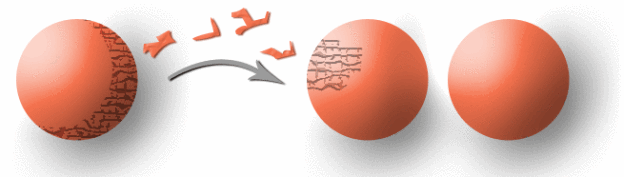
\includegraphics{figure/banach_tarski.png}

To be clear, no rule of mathematics are broken in the Banach-Tarski paradox, but the result defies intuition. Another statement of this paradox is that \emph{we can chop up a pea into finitely many pieces and reassemble it into the sun} (pea-sun paradox). If we don't lay out the foundations for measuring probabilities rigorously, we can end up with nonsensical answers!

This section was highly inspired by the following references:

\begin{itemize}
\tightlist
\item
  Rosenthal, J. (2006). A first look at rigorous probability.
\item
  The discussion here: \url{https://stats.stackexchange.com/q/199280}
\item
  This YouTube video on Vitali Sets: \url{https://youtu.be/ameugr-wjeI}
\end{itemize}

\hypertarget{conditioning-and-independence}{%
\section{Conditioning and independence}\label{conditioning-and-independence}}

In the previous section, the probabilities we encountered are \emph{unconditional}, in the sense that the probabilities do not depend on any other external factors or information, and only on the (fixed) information in the sample space.
In contrast, we may talk about \emph{conditional probabilities}.
If the sample space gets updated based on observation of new information, then this will sure impact probability calculations.

\begin{definition}[Conditional probabilities]
\protect\hypertarget{def:condprob}{}\label{def:condprob}Let \((\Omega,\cF,\bbP)\) be a probability space. For any \(A,B \in\cF\) such that \(\bbP(B)>0\), the \emph{conditional probability} of \(A\) given \(B\), written \(\bbP(A | B)\), is defined to be
\[
  \bbP(A | B) = \frac{\bbP(A \cap B)}{\bbP(B)}.
\]
\end{definition}

The event \(B\) is known as the \emph{conditioning event}.
For all intents and purposes, we may view \(\bbP(A | B)\) as ``the probability that \(A\) occurs, given that we know that \(B\) has \uline{already} occurred''.
In this sense, the given information forms an updated sample space (as \(\bbP(B | B) = 1\)):
All further occurrences are calibrated with respect to their relation to \(B\).
Thus, \(\bbP(A | B)\) as \emph{the fraction of times \(A\) occurs among those in which \(B\) occurs}.

Note that for mutually exclusive events \(A\) and \(B\), \(\bbP(A | B)=\bbP(B | A)=0\) since \(\bbP(A \cap B) = 0\).
This makes sense because as the two events are disjoint, they have ``nothing to do with each other''.

In general, \[\bbP(A | B) \neq \bbP(A).\] This is only true when dealing with independent events. Furthermore, in general \[\bbP(A | B) \neq \bbP(B | A).\]

\begin{example}
A medical test for a disease \(D\) has outcomes `\(+\)' and `\(-\)'. The probabilities are as follows:

\begin{longtable}[]{@{}lcc@{}}
\toprule
& \(D\) & \(D^c\) \\
\midrule
\endhead
\(+\) & 0.009 & 0.099 \\
\(-\) & 0.001 & 0.891 \\
\bottomrule
\end{longtable}

\emph{note: each cell represents \(\bbP(A \cap B)\).}

From the definition of conditional probability,
\[
  \bbP(+|D) = \frac{\bbP(+ \cap D)}{\bbP(D)} = \frac{0.009}{0.009 + 0.001} = 0.90
\]
and
\[
  \bbP(-|D^c) = \frac{\bbP(- \cap D^c)}{\bbP(D^c)} = \frac{0.891}{0.099 + 0.891} \approx 0.90.
\]

Suppose you go for a test and get a positive result.
What is the probability you have the disease?
Most will answer 0.90.
Actually,
\[
  \bbP(D|+) = \frac{\bbP(D \cap +)}{\bbP(+)} = \frac{0.009}{0.009 + 0.099} = 0.08.
\]
\end{example}

Notice that

\begin{itemize}
\tightlist
\item
  \(\bbP(D \cap +) = \bbP(+|D)\bbP(D)\) after some rearranging; and
\item
  \(\bbP(+) = \bbP(+ \cap D) + \bbP(+ \cap D^c)\) since \(D\) and \(D^c\) are disjoint.
\end{itemize}

We can therefore write
\[
\bbP(D|+) = \frac{\bbP(+|D)\bbP(D)}{\bbP(+|D)\bbP(D) + \bbP(+|D^c)\bbP(D^c)}.
\]
For \(\bbP(D|+)\) to be large, it seems \(\bbP(D)\) needs to be large in addition to \(\bbP(+|D)\), i.e.~disease is prevalent.

\hypertarget{bayes-theorem}{%
\subsection{Bayes Theorem}\label{bayes-theorem}}

Following that previous example, and from the definitions of conditional probabilities, we have that, after some rearranging,
\[
\bbP(A | B)\bbP(B) = \bbP(A \cap B),
\]
and
\[
\bbP(B | A) \bbP(A)= \bbP(A \cap B).
\]
So equating the two together, one can relate the two conditional probabilities \(\bbP(A | B)\) and \(\bbP(B | A)\) by
\[
\bbP(A | B) = \frac{\bbP(B|A)\bbP(A)}{\bbP(B)}.
\]

Furthermore, by using the law of total probability, we can now state Bayes' Theorem.

\begin{theorem}[Bayes' Theorem]
Let \((\Omega,\cF,\bbP)\) be a probability space, \(A_1,A_2,\dots\) a partition of the sample space, and \(B\) be any set in \(\cF\) such that \(\bbP(B)>0\).
Then, for each \(i=1,2,\dots\),
\[
  \bbP(A_i|B) = \frac{\bbP(B|A_i)\bbP(A_i)}{\sum_{j=1}^\infty \bbP(B|A_j)\bbP(A_j)}.
\]
\end{theorem}

The above rule provides a convenient way of computing conditional probability \(\bbP(A|B)\) if knowledge regarding the ``reverse'' conditional probability \(\bbP(B|A)\) is readily available.

\begin{figure}

{\centering 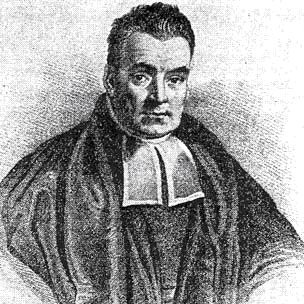
\includegraphics[width=0.5\linewidth]{figure/bayes} 

}

\caption{(Probably not) Rev. Thomas Bayes c. 1701--7 April 1761. This picture is commonly used to depict Thomas Bayes, but historians believe this not to be an accurate depiction.}\label{fig:revthomasbayes}
\end{figure}

Some will call \(\bbP(A_i)\) the \emph{prior probability}, and the \(\bbP(A_i|B)\) \emph{posterior probability}, especially in the context of Bayesian statistics. The terms refer to our state of knowledge before and after learning new information (respectively) that is used to update our beliefs.

\begin{example}
In a certain selection of flower seeds, 2/3 have been treated to improve germination and 1/3 have been left untreated.
For the purpose of this example, we may treat these numbers as probabilities of selecting a treated or untreated flower seed.

Furthermore, the seeds which have been treated have a probability of germination of 0.8, whereas the untreated seeds have a probability of germination of 0.5.

Let's calculate the probability that a seed, selected at random:

\begin{enumerate}
\def\labelenumi{(\alph{enumi})}
\tightlist
\item
  will germinate (assuming the seeds were sown and given time to germinate).
\item
  a germinated seed had been treated.
\end{enumerate}

First, let us define the following events:

\begin{itemize}
\tightlist
\item
  \(T=\) a seed has been treated
\item
  \(T^c=\) a seed has not been treated
\item
  \(G=\) a seed has germinated
\item
  \(G^c=\) a seed has not germinated
\end{itemize}

We note that the events \(T\) and \(T^c\) are disjoint and partitions the sample space (a seed can either be treated or not), and so too the case with \(G\) and \(G^c\).
After some careful reading of the question, we are actually presented with the probabilities \(\bbP(G|T)=0.8\) and \(\bbP(G|T^c)=0.5\).

To answer a., we require \(\bbP(G)\), which is obtained using the law of total probability:
\begin{align*}
\bbP(G) 
&= \bbP(G \cap T) + \bbP(G\cap T^c) \\
&= \bbP(G |T)\bbP(T) + \bbP(G|T^c)\bbP(T^c) \\
&= 2/3 \times 0.8 + 1/3 \times 0.5 = 0.7
\end{align*}

In answering b., we realise that we are after the quantity \(\bbP(T|G)\). Using Bayes' Theorem,
\begin{align*}
\bbP(T|G)
&= \frac{\bbP(G|T)\bbP(T)}{\bbP(G)} \\
&= \frac{0.8 \times 2/3}{0.7} \\
&= 0.762
\end{align*}
\end{example}

It's important to note here that \(\bbP(G|T) \neq 1 - \bbP(G|T^c)\), and this is true in most cases. We cannot take complements with respect to the conditioning event!

\hypertarget{independence}{%
\subsection{Independence}\label{independence}}

In some cases, the occurrence of a particular event \(B\) has \emph{no effect} on the probability of another event \(A\). Mathematically, we can denote this as
\[
  \bbP(A | B) = \bbP(A).
\]
If this were true, we can use the relationship \(\bbP(A \cap B) = \bbP(A | B)\bbP(B)\) to derive the following definition.

\begin{definition}
Two events \(A\) and \(B\) are \emph{statistically independent} if and only if
\[
  \bbP(A \cap B) = \bbP(A)\bbP(B).
\]
\end{definition}

What's nice about this definition is that in order to check whether to events are independent, it is sufficient to check whether their probabilities multiply out in the manner above.
Note that (and it is easily checked!) that if \(A\) and \(B\) are independent then so too are

\begin{itemize}
\tightlist
\item
  \(A\) and \(B^c\);
\item
  \(A^c\) and \(B\); and
\item
  \(A^c\) and \(B^c\).
\end{itemize}

Here's an experiment we can do to examine the concept of independent events.
Consider tossing a fair die.
Let \(A = \{2, 4, 6\}\) and \(B = \{1,2,3,4\}\).
You should be able to work out, using the above probability results and the definition of conditional probabilities, that \(\bbP(A)=1/2\), \(\bbP(B)=2/3\), and \(\bbP(A \cap B)=1/3\).
Hence, we deduce that \(A\) and \(B\) are independent, since the product of each probability event is the probability of their intersection.

If you were feeling bored and had a lot of time to spare, you could verify this empirically using an actual die.
While this would be an afternoon well spent, let's use \texttt{R} to simulate some draws from the sample space \(\Omega = \{1,2,3,4,5,6\}\), and count the number of times each events \(A\), \(B\) and \(A \cap B\) occurs.

\begin{Shaded}
\begin{Highlighting}[]
\CommentTok{\# Throw a dice 10 times}
\FunctionTok{sample}\NormalTok{(}\DecValTok{1}\SpecialCharTok{:}\DecValTok{6}\NormalTok{, }\AttributeTok{size =} \DecValTok{10}\NormalTok{, }\AttributeTok{replace =} \ConstantTok{TRUE}\NormalTok{)}
\end{Highlighting}
\end{Shaded}

\begin{verbatim}
##  [1] 3 6 3 2 2 6 3 5 4 6
\end{verbatim}

From the above, \(n(A) = 6\), \(n(B)=6\), and \(n(A \cap B)=3\).
Here I've used the notation \(n(\cdot)\) to mean the count of the event.
Do this 1,000 times, and count events automatically using the following code.

\begin{Shaded}
\begin{Highlighting}[]
\NormalTok{x }\OtherTok{\textless{}{-}} \FunctionTok{sample}\NormalTok{(}\DecValTok{1}\SpecialCharTok{:}\DecValTok{6}\NormalTok{, }\AttributeTok{size =} \DecValTok{1000}\NormalTok{, }\AttributeTok{replace =} \ConstantTok{TRUE}\NormalTok{)}
\FunctionTok{head}\NormalTok{(x, }\DecValTok{100}\NormalTok{)  }\CommentTok{\# show the first 100 outcomes}
\end{Highlighting}
\end{Shaded}

\begin{verbatim}
##   [1] 6 1 2 3 5 3 3 1 4 1 1 5 3 2 2 1 6 3 4 6 1 3 5 4 2 5 1 1 2 3 4 5 5 3 6 1 2
##  [38] 5 5 4 5 2 1 1 3 1 6 5 1 2 4 4 6 6 3 6 6 1 6 2 1 2 4 5 5 6 3 1 4 6 1 6 1 3
##  [75] 6 4 1 6 6 3 6 5 3 6 2 5 5 3 2 2 2 4 2 2 6 4 4 6 1 6
\end{verbatim}

\begin{Shaded}
\begin{Highlighting}[]
\NormalTok{nA }\OtherTok{\textless{}{-}} \FunctionTok{sum}\NormalTok{(x }\SpecialCharTok{\%in\%} \FunctionTok{c}\NormalTok{(}\DecValTok{2}\NormalTok{, }\DecValTok{4}\NormalTok{, }\DecValTok{6}\NormalTok{))  }\CommentTok{\# counts the frequency of 2, 4, 6}
\NormalTok{nB }\OtherTok{\textless{}{-}} \FunctionTok{sum}\NormalTok{(x }\SpecialCharTok{\%in\%} \FunctionTok{c}\NormalTok{(}\DecValTok{1}\NormalTok{, }\DecValTok{2}\NormalTok{, }\DecValTok{3}\NormalTok{, }\DecValTok{4}\NormalTok{))  }\CommentTok{\# counts the frequency of 1, 2, 3, 4}
\NormalTok{nAB }\OtherTok{\textless{}{-}} \FunctionTok{sum}\NormalTok{(x }\SpecialCharTok{\%in\%} \FunctionTok{c}\NormalTok{(}\DecValTok{2}\NormalTok{, }\DecValTok{4}\NormalTok{))  }\CommentTok{\# counts the frequency of 2, 4}

\CommentTok{\# Results}
\FunctionTok{c}\NormalTok{(}\AttributeTok{A =}\NormalTok{ nA, }\AttributeTok{B =}\NormalTok{ nB, }\AttributeTok{AnB =}\NormalTok{ nAB) }\SpecialCharTok{/} \DecValTok{1000}
\end{Highlighting}
\end{Shaded}

\begin{verbatim}
##     A     B   AnB 
## 0.495 0.674 0.333
\end{verbatim}

Empirically, we have \(\hat{\bbP}(A)\hat{\bbP}(B) =\) 0.495 \(\times\) 0.674\(=\) 0.33363.
This matches with the value of \(\hat{\bbP}(A \cap B)\) in the table, as well as the theoretical value of 1/3.

\hypertarget{random-variables}{%
\section{Random variables}\label{random-variables}}

Consider the following problem:
Ask (randomly) 50 people whether they like (code this as ``1'') or dislike (code this as ``0'') learning statistics.
What is the sample space for this experiment?
This would be all 1/0 combinations such as

\begin{align*}
\overbrace{1000101\cdots 10001}^{50}
\end{align*}
Specifically, \(\Omega = \big\{(X_1,X_2,\dots,X_{50}) \,|\, X_i \in \{0,1\} \big\}\). Realise that \(|\Omega| = 2^{50}\). This is huge\footnote{For context, the average American, working full-time, would have to work 25 billion years to earn 1 quadrillion dollars.}!

\begin{Shaded}
\begin{Highlighting}[]
\DecValTok{2} \SpecialCharTok{\^{}}\NormalTok{ \{}\DecValTok{50}\NormalTok{\}}
\end{Highlighting}
\end{Shaded}

\begin{verbatim}
## [1] 1.1259e+15
\end{verbatim}

Is it practical to work with such a large sample space?
Possibly not, even with fancy counting techniques.

But what if we instead defined a variable \(Y = \sum_{i=1}^{50} X_i\)?
Here, \(Y\) is the count of the number of people who like learning statistics from this sample of 50, since it only counts the values of '1's occuring.
Further, the minimum value for \(Y\) is 0, and the maximum is 50.
So the new sample space associated with \(Y\) is \(S=\{0,1,2,\dots,50\}\)--much easier to deal with!

\(Y\) is defined to be a mapping from the original sample space \(\Omega\) to the new space \(S\) (usually a set of real numbers).
Such a mapping is called a \textbf{random variable}.

\begin{definition}[Random variable]
A \emph{random variable} \(X\) (abbreviated r.v.) on a probability space \((\Omega,\cF,\bbP)\) is a \emph{measurable function}\footnote{A measurable function is simply a function between the underlying sets of two measurable spaces. This will help preserve the structure of the spaces and allow things to be measured. See Wasserman, Appendix 2.13.} from \((\Omega,\cF)\) to \(\bbR\), i.e.~\(X:\Omega\to\bbR\).
\end{definition}

This is much easier exaplained with an example.

\begin{example}

Flip a coin twice and let \(X\) be the number of heads.
The sample space of the coin flips is \(\Omega = \{\text{HH}, \text{HT}, \text{TH}, \text{TT} \}\).
The sample space of \(X\) is \(S = \{0,1,2 \}\).
The mapping of the random variable is illustrated as follows:

\begin{center}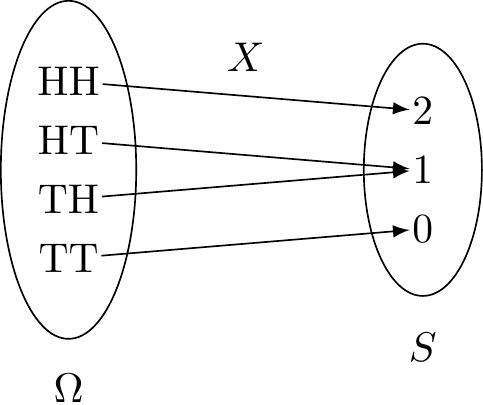
\includegraphics[width=0.48\linewidth]{bookdown-adv-stats_files/figure-latex/unnamed-chunk-4-1} \end{center}

\end{example}

The qualifier \emph{random} to the term `random variable' implies that its value is not known before observing it.
Random variables are conventionally denoted with uppercase letters, and the realised values of the variable will be denoted by the corresponding lowercase letters. Thus, the random variable \(X\) can take the value \(x\).

We can see that a r.v. \(X\) assigns a real number \(X(\omega)\) to each outcome \(\omega\).
Can we still calculate probabilities of events? Yes.
\[
  \bbP(X=x) = \bbP\big(X^{-1}(x)\big) = \bbP\big(\{ \omega \in \Omega \,|\, X(\omega) = x\} \big)
\]
More generally,
\[
  \bbP(X\in S) = \bbP\big(X^{-1}(x)\big) = \bbP\big(\{ \omega \in \Omega \,|\, X(\omega) \in S \} \big)
\]

\begin{example}
\protect\hypertarget{exm:coinflip}{}\label{exm:coinflip}For the previous example, the random variable \(X\) can be summarised as follows:

\begin{longtable}[]{@{}ccc@{}}
\toprule
\(\omega\) & \(\bbP(\{\omega\})\) & \(X(\omega)\) \\
\midrule
\endhead
TT & 1/4 & 0 \\
TH & 1/4 & 1 \\
HT & 1/4 & 1 \\
HH & 1/4 & 2 \\
\bottomrule
\end{longtable}

\begin{longtable}[]{@{}ccc@{}}
\toprule
\(x\) & \(\bbP(X = x)\) & \(X^{-1}(x)\) \\
\midrule
\endhead
0 & 1/4 & TT \\
1 & 1/2 & TH, HT \\
2 & 1/4 & HH \\
\bottomrule
\end{longtable}

In either case, the sum of the probabilities, whether in the original event space \(\Omega\) or in the range of the random variable \(S\), is equal to one.
\end{example}

\hypertarget{distribution-functions}{%
\subsection{Distribution functions}\label{distribution-functions}}

With every random variable \(X\), we associate a function called the cumulative distribution function of \(X\).

\begin{definition}
The \emph{cumulative distribution function (cdf)} of a r.v. \(X\), denoted \(F_X\), is the function \(F_X:\bbR\to[0,1]\) defined by
\[
  F_X(x) = \bbP(X \leq x), \text{ for all } x.
\]
The cdf is sometimes just referred to as the \emph{distribution function}.
When there is no ambiguity regarding which random variable the cdf is referring to, we may drop the subcript in \(F_X\).
\end{definition}

Equivalently, the distribution function is written
\[
F_X(x) = \bbP\left(\{\omega \in \Omega \mid X(\omega) \leq x \} \right).
\]

We make some observations regarding the distribution function:

\begin{itemize}
\tightlist
\item
  \(\lim_{x\to-\infty} F(x) = 0\) and \(\lim_{x\to+\infty} F(x) = 1\).
\item
  \(F(x)\) is non-decreasing, i.e.~\(x_1 < x_2 \Rightarrow F(x_1) \leq F(x_2)\). In other words, drawing the function from left to right, it must either increase or stay the same value, but not decrease in value.
\item
  \(F(x)\) is right-continuous: for every \(x_0\), \(\lim_{x \downarrow x_0} F(x) = F(x_0)\). This means ``the solid dots will be on the left of the distribution function''.
\item
  \(F\) itself \emph{can be discontinuous} (see the next example). This is associated with whether the r.v. \(X\) is continuous or not. That is,

  \begin{itemize}
  \tightlist
  \item
    \(F_X(x)\) is a continuous function \(\Rightarrow\) \(X\) is continuous.
  \item
    \(F_X(x)\) is a step function \(\Rightarrow\) \(X\) is discrete.
  \end{itemize}
\end{itemize}

\begin{figure}

{\centering 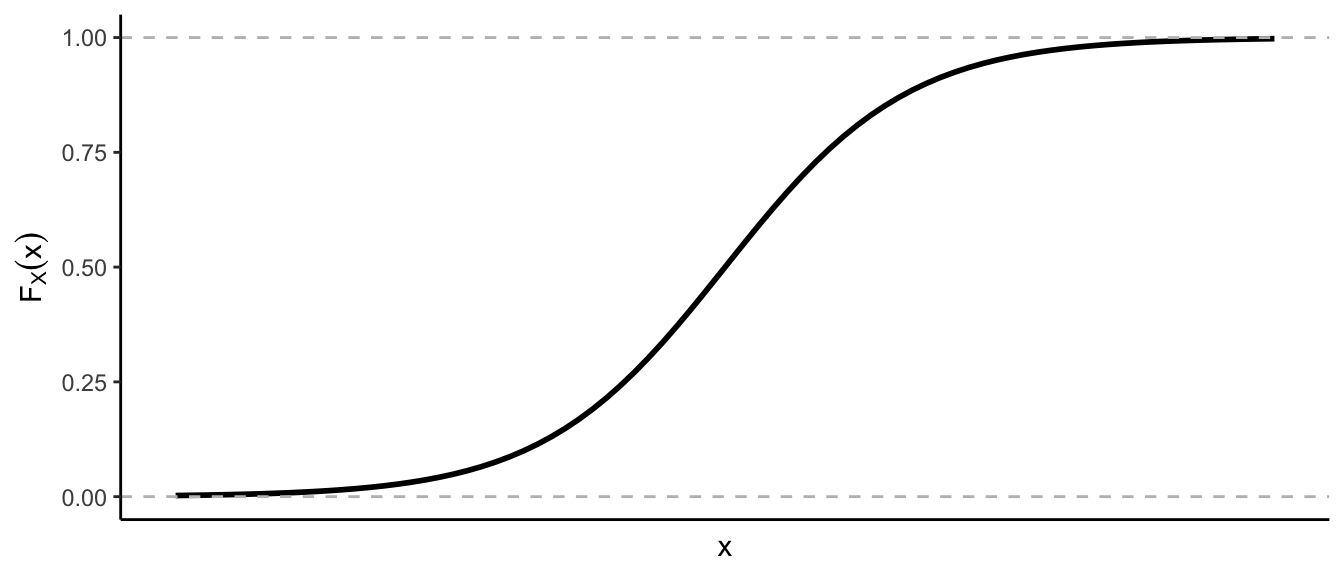
\includegraphics[width=1\linewidth]{bookdown-adv-stats_files/figure-latex/generalcdf-1} 

}

\caption{A general sketch of a (continuous) cdf.}\label{fig:generalcdf}
\end{figure}

Once again, the definition above does not give a functional form for the cdf, but the good news is that any function satisfying the above properties is a cdf. For proofs of these facts, see the reference textbooks.

\begin{example}

From Example \ref{exm:coinflip}, we have that
\[
F_X(x)=
\begin{cases}
0   &x < 0 \\
0.25  &0 \leq x < 1 \\
0.75  &1 \leq x < 2 \\
1  &x \geq 2 \\
\end{cases}
\]

This can be sketched as follows:

\begin{center}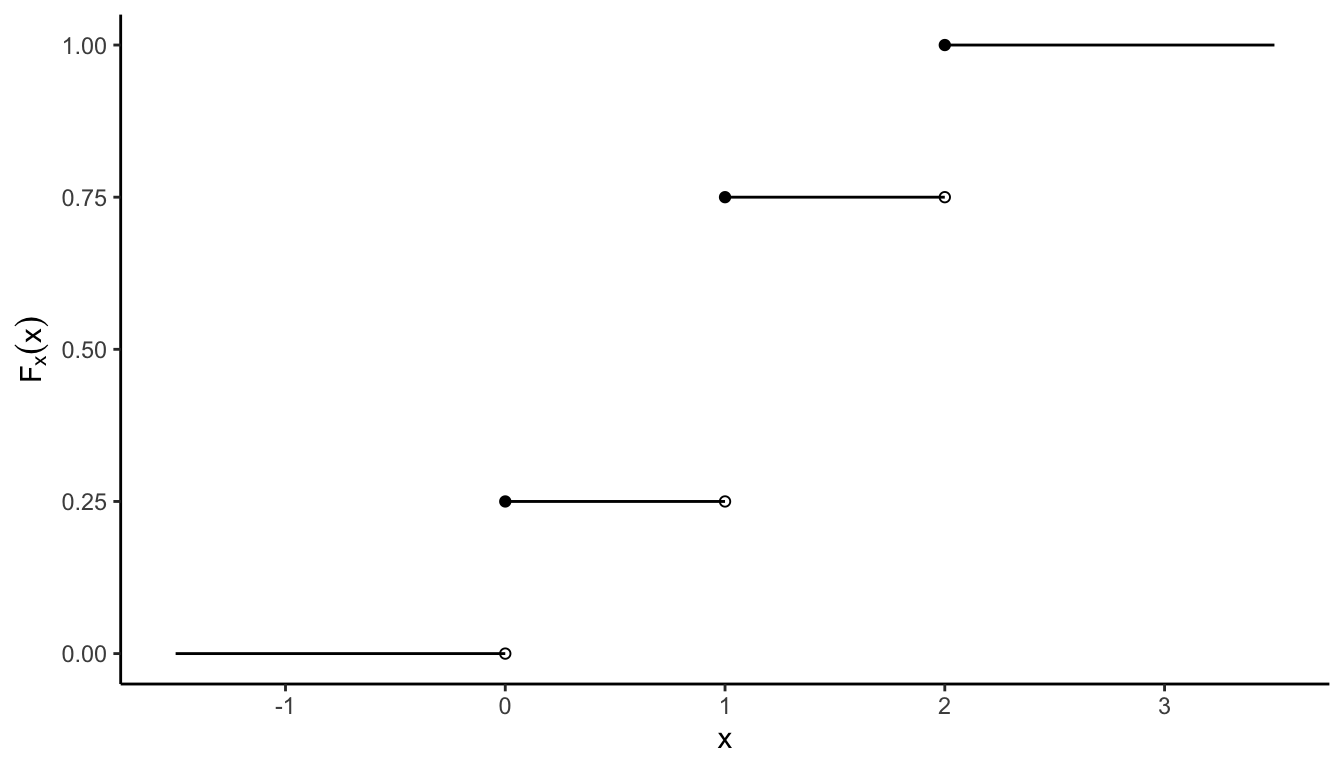
\includegraphics[width=1\linewidth]{bookdown-adv-stats_files/figure-latex/distfn-1} \end{center}

\end{example}

\hypertarget{identically-distributed-r.v.}{%
\subsection{Identically distributed r.v.}\label{identically-distributed-r.v.}}

\begin{definition}[Identically distributed r.v.]
Let \(X\) have cdf \(F\) and let \(Y\) have cdf \(G\).
If \(F(x)=G(x)\) for all \(x\), then \(\bbP(X\in A) = \bbP(Y \in A)\) for all (measurable) sets \(A\).
\(X\) and \(Y\) are said to be \emph{identically distributed}.
\end{definition}

Note that two identically distributed r.v. are not necessarily equal in value, only the probabilities of observing the same values are identical.
Think about two independent coin flips. The probability of H/T in each flip is the same, but the outcome may not be.

\begin{example}
Consider again the experiment of tossing a coin twice.
Define the random variables \(X\) and \(Y\) to be the number of heads and tails observed, respectively.
The distribution of \(X\), as we calculated previously, is

\begin{longtable}[]{@{}cccc@{}}
\toprule
\(x\) & 0 & 1 & 2 \\
\midrule
\endhead
\(\bbP(X=x)\) & 1/4 & 1/2 & 1/4 \\
\bottomrule
\end{longtable}

One can easily verify that the distribution of \(Y\) is

\begin{longtable}[]{@{}cccc@{}}
\toprule
\(y\) & 0 & 1 & 2 \\
\midrule
\endhead
\(\bbP(Y=y)\) & 1/4 & 1/2 & 1/4 \\
\bottomrule
\end{longtable}

Thus, for each \(k=0,1,2\), \(\bbP(X=k)=\bbP(Y=k)\), so \(X\) and \(Y\) are identically distributed.
\end{example}

\hypertarget{probability-functions}{%
\section{Probability functions}\label{probability-functions}}

Going forward, we will be concentrating more on random variables and their distributions, rather than working in a probability space.
While this is the case, hopefully you appreciate the probability theory that is going on behind the scenes.

Associated with a random variable \(X\) and its cdf \(F_X\) is another function, called either the probability density function (pdf) if it is continuous, or the probability mass function (pmf) if it is discrete.
We shall look at both in turn.

\hypertarget{probability-mass-function}{%
\subsection{Probability mass function}\label{probability-mass-function}}

\begin{definition}[Probability mass function]
A \uline{discrete} random variable \(X\) may only take countably many values \(\cX = \{x_1, x_2,\dots \}\).
Its \emph{probability mass function (pmf)} is defined to be
\[
f_X(x) = \bbP(X=x), \text{ for all } x \in \cX.
\]
\end{definition}

The pmf is a function which takes input possible values that a random variable may take, and outputs the probability that the random variable takes that value.
An example is given below.

\begin{example}

The pmf from Example \ref{exm:coinflip} (the two coin flips) is given by

\[
f_X(x) = \begin{cases}
1/4&x=0 \\
1/2&x=1 \\
1/4& x=2\\
0 &\text{otherwise}\\
\end{cases}
\]

\begin{center}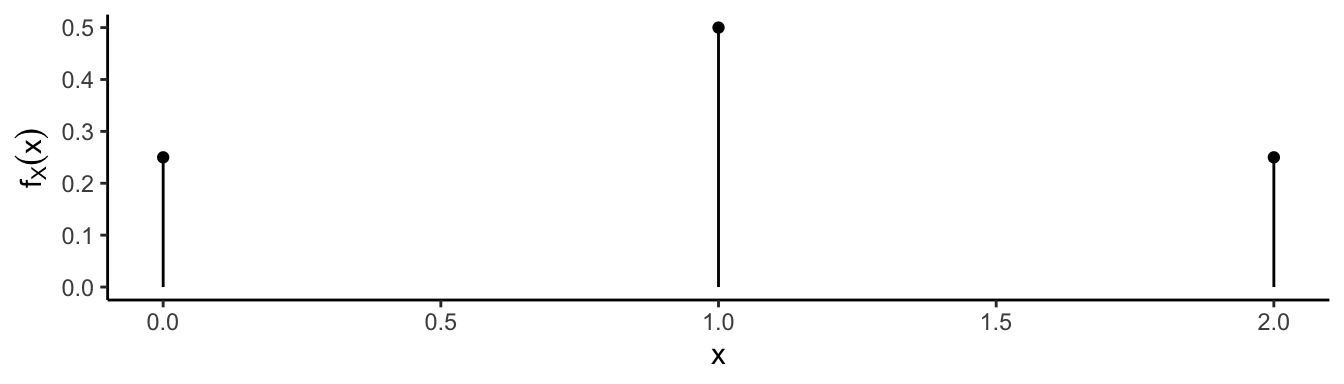
\includegraphics[width=1\linewidth]{bookdown-adv-stats_files/figure-latex/unnamed-chunk-5-1} \end{center}

\end{example}

Pmfs measure ``point probabilities''. Since outcomes of discrete random variables are countable, we can add up probabilities over all the points in the event.
That is, for any \(a\), \(b\) both in \(\cX\) such that \(a \leq b\), we have that
\begin{align*}
\bbP(a \leq X \leq b) 
&= \bbP(X=a) + \cdots + \bbP(X=b) \\
&= \sum_{x=a}^b f_X(x) 
\end{align*}

As a special case we get
\begin{equation}
\bbP(X \leq b) = \sum_{x\leq b} f_X(x) = F_X(b). \label{eq:discretecdfpmf}
\end{equation}

Consequently, we notice that each \(f_x(x) \geq 0\) for all \(x\) (since they are probabilities), and that \(\sum_{x} f_x(x) = 1\), as this is summing over the entire sample space of \(X\).

\hypertarget{probability-density-functions}{%
\subsection{Probability density functions}\label{probability-density-functions}}

We would like to translate the very same idea of ``point probabilities'' over from the discrete case to the continuous case, but in doing so must exercise caution.
Let \(X\) be a continuous random variable. i.e.~\(X\) is a random variable whose cdf is continuous.
If such a probability function \(f_X\) exists for \(X\), then the analogous procedure would be to consider
\[
  \bbP(X \leq x) = F_X(x) = \int_{-\infty}^x f_X(x) \dint \tilde x,
\]
as this would be like summing over all possible values of \(f_X(x)\) such that \(X\leq x\) on a continuous scale\footnote{The Riemann integral is defined as the limit of the sum of the areas of bars dividing the area under the curve, as the number of bars gets larger and larger (and hence the width of the bars get smaller and smaller).}, as per \eqref{eq:discretecdfpmf}.
In essence, the cdf \(F_X\) acts to ``add up'' all the ``point probabilities'' \(f_X\) within a required interval.

\begin{definition}[Probability density function]
A \uline{continuous} random variable \(X\) takes any numerical value within in an interval or collection of intervals (having an uncountable range).
Its \emph{probability density function (pdf)} is the function \(f_X(x)\) that satisfies
\[
F_X(x) = \int_{-\infty}^x f_X(\tilde x) \dint \tilde x, \text{ for all } x.
\]
\end{definition}

Geometrically speaking, the cdf computes the area under the pdf up to a point \(x\), as shown in the diagram below:

\begin{figure}

{\centering 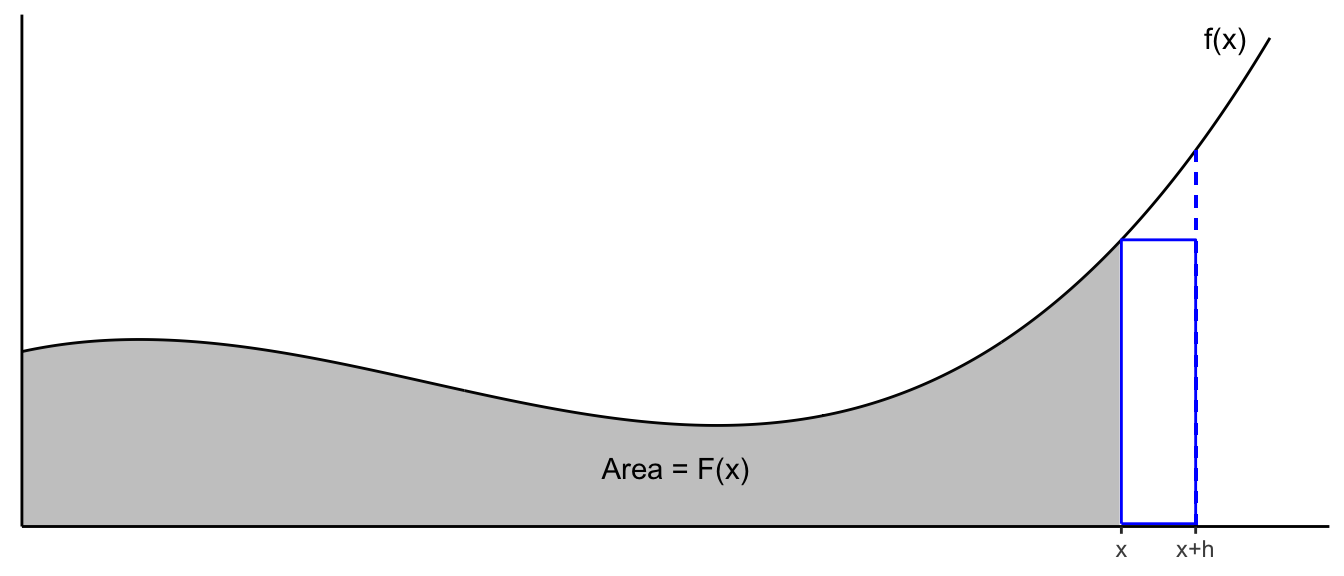
\includegraphics[width=1\linewidth]{bookdown-adv-stats_files/figure-latex/areaunderpdf-1} 

}

\caption{Illustration of the cdf as being the area under the pdf curve.}\label{fig:areaunderpdf}
\end{figure}

Consider the area under the curve up to the point \(x+h\).
This is given by \(F(x+h)\), but may also be approximated as \(F(x+h) \approx F(x) + A_{blue}\), where \(A_{blue}=f(x)\cdot h\) is the area of the blue rectangle.
This might be a poor approximation, and is only ever a good one when \(h\) is small.
With a little rearranging, we get
\[
f(x) \approx \frac{F(x+h)-F(x)}{h}
\]
and argue that the RHS approaches the quantity \(f(x)\) as \(h\) tends to zero, i.e.
\[
f(x) = \lim_{h\to 0} \frac{F(x+h)-F(x)}{h},
\]
which is the definition of the derivative.
This is the idea of the Fundamental Theorem of Calculus, which tells us that
\[
  f_X(x) = \frac{\ddif}{\ddif x}F_X(x).
\]

Several observations regarding the probability density function:

\begin{itemize}
\tightlist
\item
  \(f_X(x) \geq 0\) for all \(x\). The curve of the pdf cannot dip below the \(x\)-axis.
\item
  \(\int_{-\infty}^\infty f_X(x) \dint x = 1\), which is essentially saying \(\bbP(\Omega)=1\).
\item
  Point probabilities have no weight in the continuous case: \[\bbP(X=x) = \int_x^x f(\tilde x) \dint \tilde x = 0.\] In effect, we can be less strict about the use of inequalities, since

  \begin{itemize}
  \tightlist
  \item
    \(\bbP(X \leq b) = \bbP(X <b) + \cancel{\bbP(X=b)}\); and thus
  \item
    \(\bbP(a \leq X \leq b) = \bbP(a \leq X < b) = \bbP(a < X \leq b) = \bbP(a < X < b)\).
  \end{itemize}
\item
  To calculate probabilities within an interval, we can do the following:

  \begin{itemize}
  \tightlist
  \item
    \(\bbP(a<X<b) = F(b) - F(a)\) (be careful, this is not true for discrete r.v.)
  \item
    \(\bbP(X > a) = 1 - F(a)\)
  \end{itemize}
\end{itemize}

It's wrong to think of pdfs \(f(x)\) as probability functions--this only holds for discrete r.v..
Continuous pdfs do not give us probabilities unless we perform definite integrals on them.
Read Wasserman (Warning after Example 2.13 on p.24) for more on this.

\begin{example}

Suppose that \(X\) is uniformly distributed on the interval \((a,b) \subset \bbR\).
Its pdf is given by
\[
f_X(x) = \begin{cases}
\frac{1}{b-a} & a < x < b \\
0 & \text{otherwise}
\end{cases}
\]

When \(a < x < b\), the cdf is
\begin{align*}
F_X(x) 
= \int_{-\infty}^x f_X(\tilde x) \dint \tilde x 
&=\cancelto{0}{\int_{-\infty}^a f_X(\tilde x) \dint \tilde x}  + \int_{a}^x \frac{1}{b-a} \dint \tilde x \\
&= \left[ \frac{\tilde x}{b-a} \right]_a^x = \frac{x-a}{b-a},
\end{align*}
while \(F_X(x) = 0\) for \(x<a\), and \(F_X(x)=1\) for \(x>b\).

\begin{center}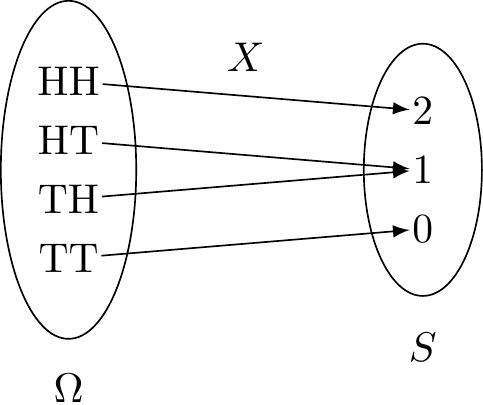
\includegraphics[width=1\linewidth]{bookdown-adv-stats_files/figure-latex/unnamed-chunk-6-1} \end{center}

\begin{center}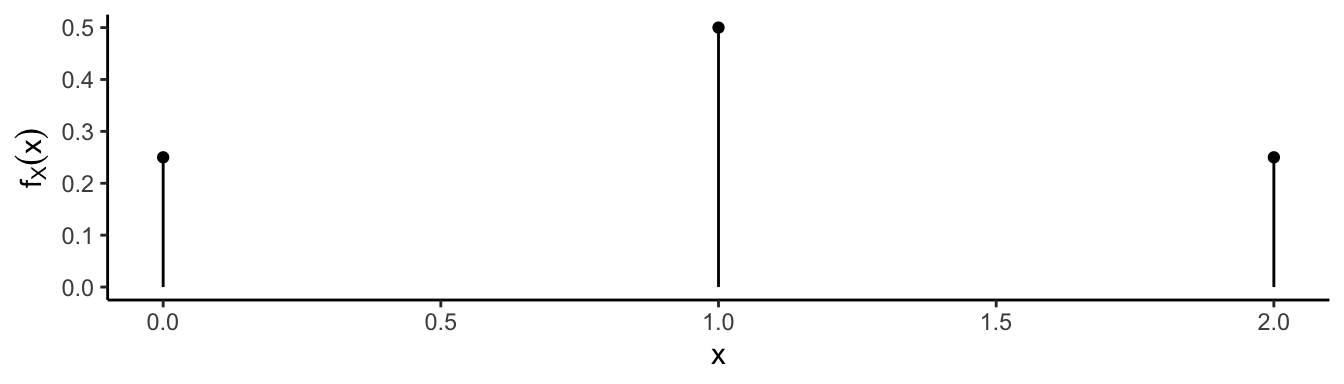
\includegraphics[width=1\linewidth]{bookdown-adv-stats_files/figure-latex/unnamed-chunk-7-1} \end{center}

\end{example}

Just some remarks on notation:

\begin{enumerate}
\def\labelenumi{\arabic{enumi}.}
\item
  We write \(X \sim F_X(x)\) to mean that ``\(X\) has a distribution given by \(F_X(x)\)''.
  The symbol `\(\sim\)' is read ``is distributed as''.
  Sometimes writing it with the pdf \(X \sim f_X(x)\) is also clear in meaning.
  If we are dealing with a commonly used probability distribution, we would use their specially given name, e.g.~\(X\sim \Unif(a,b)\).
  If \(X\) and \(Y\) are identically distributed, then we write \(X\sim Y\).
\item
  Sometimes we just write \(\int f(x) \dint x\) to mean \(\int_{-\infty}^{\infty} f(x) \dint x\).
\end{enumerate}

In case you were wondering, random variables with mixed distributions do exist, but we won't really encounter them in this course.
Here's some food for thought.
Let \(X\) be a discrete random variable (e.g.~one that follows the two coin flip distribution), and let \(Y\) be a continuous random variable (e.g.~a uniform distribution on the interval \([0,1]\)).
Construct a new random variable \(Z\) by flipping a fair coin and define
\[
Z = \begin{cases}
X & \text{coin lands Heads} \\
Y & \text{coin lands Tails}
\end{cases}
\]
Since the probability of a coin toss is 50-50, in symbols we can write \(\bbP(Z=X)=\bbP(Z=Y)=0.5\).
The question is, what sort of random variable is \(Z\)?
If it is discrete, then how can it take on uncountably many different values when the coin lands tails?
If it is continuous, then how come the point probability \(\bbP(Z=X)=1/2\) is non-zero?

The good news here is that categorising a random variable as discrete or continuous is purely arbitrary and convenient, but not required at all when measure theoretic foundations are used.
There is no issue at all when dealing with such random variables, as the measure space will be well defined.

\hypertarget{transformations}{%
\section{Transformations}\label{transformations}}

In statistics, it is often the case that given a random variable \(X\), we are also interested in transformations of this random variable.
For example, if \(X\) is made to represent the gross domestic product (GDP) of a country, then we may be interested to study the logarithm of the GDP instead.

If \(X\sim F_X(x)\) is a random variable, then a transformation of \(X\) by any function, \(g(X)\) say, is also a random variable.
Writing \(Y=g(X)\), we may describe the probabilistic behaviour of \(Y\) in terms of that of X:
\begin{equation}
\bbP(Y\in A) = \bbP(g(X)\in A). \label{eq:probtransform1}
\end{equation}
Sometimes we may write this expression explicitly, but is this always the case?
It really depends on the transformation \(g\).

Formally, \(g\) defines a mapping a from the original sample space of \(X\) (let's denote this \(\cX\)) to a new sample space \(\cY\) for \(Y\).
We can write \(g:\cX\to\cY\).
For random variable \(X\) and its transformed version \(Y=g(X)\), these sets are
\[
\cX = \{ x \mid f_X(x) > 0\} \hspace{1em}\text{and}\hspace{1em} \cY = \{y \mid y=g(x) \text{ for } x\in\cX \}.
\]
The set \(\cX\) is called the \emph{support} of the random variable \(X\); the points at which the distribution is valid.
We associate with \(g\) an \emph{inverse mapping} denoted by \(g^{-1}:\cY\to\cX\), defined by
\[
g^{-1}(A) = \{ x \in \cX \mid g(x) \in A \}.
\]
Then the probability in \eqref{eq:probtransform1} can be written as
\[
\bbP(Y\in A) = \bbP\big(X\in g^{-1}(A)\big).
\]

For discrete random variables, this is relatively straightforward, as seen in the following example.

\begin{example}
Let \(X\) be a random variable with a discrete uniform distribution on the set \(\{-1,0,1\}\). That is,
\[
f_X(x) = \begin{cases}
1/3 & x \in \{-1,0,1\} \\
0 & \text{otherwise.}
\end{cases}
\]
Consider the transformation \(Y=X^2\). Then the values of \(Y\) are
\[
Y = \begin{cases}
0 & X=0\\
1 & X =-1,1\\
\end{cases}
\]
and they take these values with probabilities
\[
\bbP(Y=0) = \bbP(X=0) = 1/3,
\]
and
\[
\bbP(Y=1) = \bbP(X=-1) + \bbP(X=1) = 1/3 + 1/3 = 2/3.
\]
As a remark, \(Y\) takes fewer values than \(X\) because the transformation is not one-to-one.
\end{example}

The continuous case is harder, and we need to consider the type of function and also keep track of the sample space.
Suppose \(x \mapsto g(x)\) represents a strictly monotonic transformation from \(\cX\) to \(\cY\).
This means that \(g\) is both \emph{injective} (one-to-one) and \emph{surjective} (onto); meaning that \(g\) is \emph{bijective}.
Importantly, \(g\) can be \textbf{inverted}.

\begin{figure}

{\centering 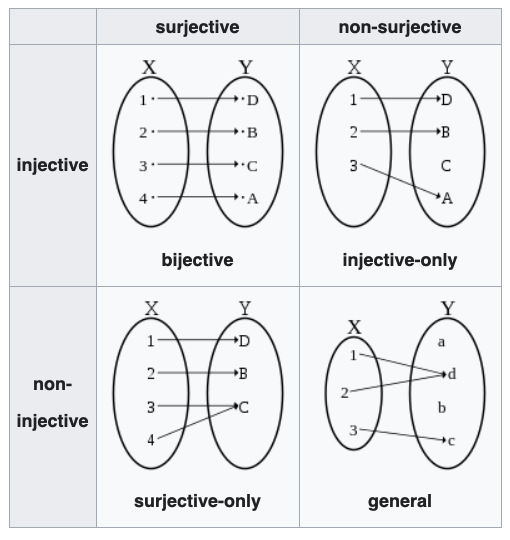
\includegraphics[width=0.6\linewidth]{figure/bijective} 

}

\caption{Injective vs surjective functions.}\label{fig:bijective}
\end{figure}

We can work out the cdf of \(Y\) when \(g\) is increasing:
\begin{align}
F_Y(y) 
&= \bbP(Y \leq y) \nonumber \\
&= \bbP\big(g(X) \leq y\big)  \nonumber \\
&= \bbP\big(X \leq g^{-1}(y)\big)  \nonumber \\
&= F_X\big(g^{-1}(y)\big) \label{eq:cdftransform1}
\end{align}

On the other hand, when \(g\) is decreasing:
\begin{align}
F_Y(y) 
&= \bbP(Y \leq y)  \nonumber \\
&= \bbP\big(g(X) \leq y\big) \nonumber \\
&= \bbP\big(X > g^{-1}(y)\big) \hspace{1em} \rlap{\text{note the sign reversal}}  \nonumber \\
&= 1 - F_X\big(g^{-1}(y)\big) \label{eq:cdftransform2}
\end{align}

The above is somewhat of an informal derivation of the cdf of the transformed variable \(Y\).
For more mathematical details, please see C\&B Section 2.1.
The main message here is that we need to keep track of the set \(A_y=\{x \in \cX \mid g(x) \leq y \}\), and it depends on whether or not \(g\) is increasing or decreasing.
From here, the pdf of \(Y\) can be obtained by differentiating the cdf (in the continuous case).
The following theorem formalises this approach.

\begin{theorem}[Pdf of continuous transformations]
Let \(X\) have pdf \(f_X(x)\) and let \(Y=g(X)\) be a strictly monotone function, i.e.~\(g\) is strictly increasing or decreasing.
Suppose also that \(f_X(x)\) is continuous on the support of \(X\), and that the inverse \(g^{-1}(y)\) has a continuous derivative on the support of \(Y\).
Then the pdf of \(Y\) is given by
\[
f_Y(y) = \begin{cases}
f_X\big(g^{-1}(y)\big) \left| \frac{\ddif}{\ddif y}g^{-1}(y) \right| & y \in \{y\mid y=g(x) \text{ s.t. } f_X(x)>0\} \\
0 &\text{otherwise}
\end{cases}
\]
\end{theorem}

Note that the pdf of \(Y\) is valid everywhere the inverse transformation is valid on the pdf of \(X\).
For example, if \(X\) has support \(\bbR\), then \(Y=X^2\) has support only on \([0,\infty)\).

\begin{proof}
Differentiate and apply the chain rule to \eqref{eq:cdftransform1} and \eqref{eq:cdftransform2}:

\[
f_Y(y)=\frac{\ddif}{\ddif y} = \begin{cases}
f_X\big(g^{-1}(y)\big)  \frac{\ddif}{\ddif y}g^{-1}(y) &g \text{ increasing} \\
-f_X\big(g^{-1}(y)\big)  \frac{\ddif}{\ddif y}g^{-1}(y) &g \text{ decreasing.}
\end{cases}
\]
\end{proof}

\begin{example}
Let \(X\sim\Unif(-1,1)\) (continuous). The pdf of \(X\) is given by
\[
f_X(x) = \begin{cases}
1/2 & x \in (-1,1) \\
0 & \text{otherwise.}
\end{cases}
\]
Let \(Y=X^2\).
By symmetry, \(|X|\sim\Unif(0,1)\); and \(Y=|X|^2\) is a smooth, invertible function of \(|X|\). Hence
\begin{align*}
f_Y(y) 
&= f_{|X|}(\sqrt y)\left| \frac{\ddif}{\ddif y} \sqrt y \right| \\
&= 1 \cdot \frac{1}{2\sqrt y}
\end{align*}
for \(0<y<1\).
Note however, \(Y=X^2\) is not uniformly distributed anymore.
\end{example}

\hypertarget{probability-integral-transform}{%
\subsection{Probability integral transform}\label{probability-integral-transform}}

A special and very useful kind of transformation is the \emph{probability integral transform (PIT)}.
Suppose \(X\) is continuous, and let \(Y=F_X(X)\).
Here, \(Y\) is transformed using the cdf of \(X\), and is considered a random variable still because it's a function of a random variable.
Then, the distribution of \(Y\) is uniform on \((0,1)\)!

\begin{theorem}[Probability integral transform (PIT)]
Let \(X\) have continuous cdf \(F_X(x)\) and define the random variable \(Y\) as \(Y=F_X(X)\). Then \(Y\) is uniformly distributed on \((0,1)\), that is, \(Y\sim\Unif(0,1)\) and
\[
f_Y(y) = \begin{cases}
1 & 0<y<1\\
0 & \text{otherwise} \\
\end{cases}
\]
with \(\bbP(Y\leq y)=y=F_Y(y)\) for \(y\in(0,1)\).
\end{theorem}

\begin{proof}

For \(Y=F_X(X)\) we have, for \(0<y<1\),
\begin{align*}
\bbP(Y \leq y)
&= \bbP\big(F_x(X) \leq y\big) \\
&= \bbP\big(X \leq F^{-1}_X(y) \big) \\
&= F_X\big( F^{-1}_X(y) \big) \\
&= y.
\end{align*}

At the endpoints we have \(\bbP(Y \leq y) = 1\) for \(y\geq 1\) and \(\bbP(Y \leq y) = 0\) for \(y\leq 0\), since there is zero probability outside the interval \((0,1)\).
Thus \(Y\) has a uniform distribution.

Note that in the above proof, we used the fact that \(F_X\) is a monotone increasing function, and thus the equality
\[
\bbP\big(F^{-1}_X(F_X(X)) \leq F^{-1}_X(y) \big) = \bbP\big(X \leq F^{-1}_X(y) \big)
\]
holds. There are two cases:

\begin{itemize}
\item
  Suppose \(F_X\) is strictly increasing. Then it is true that \(F^{-1}_X(F_X(x))=x\), since the inverse is uniquely defined.
\item
  Suppose \(F_X\) is increasing but with ``flat'' parts. Then there are regions \(A\) of the cdf where the inverse is not uniquely defined. But for \(x\in A\), the above equality still holds true because \(\bbP(X\leq x) = \bbP(X \leq x^*) = y^*\), where \(x^* = \inf\{x | x\in A, F_X(x) = y^* \}\). In essence, the flat cdf denotes a region of 0 probability. For instance, suppose the region \(A=[x_1,x_2]\). Then \(\bbP(X\leq x) = \bbP(X \leq x_1)\) for any \(x \in A\).
\end{itemize}

\begin{figure}

{\centering 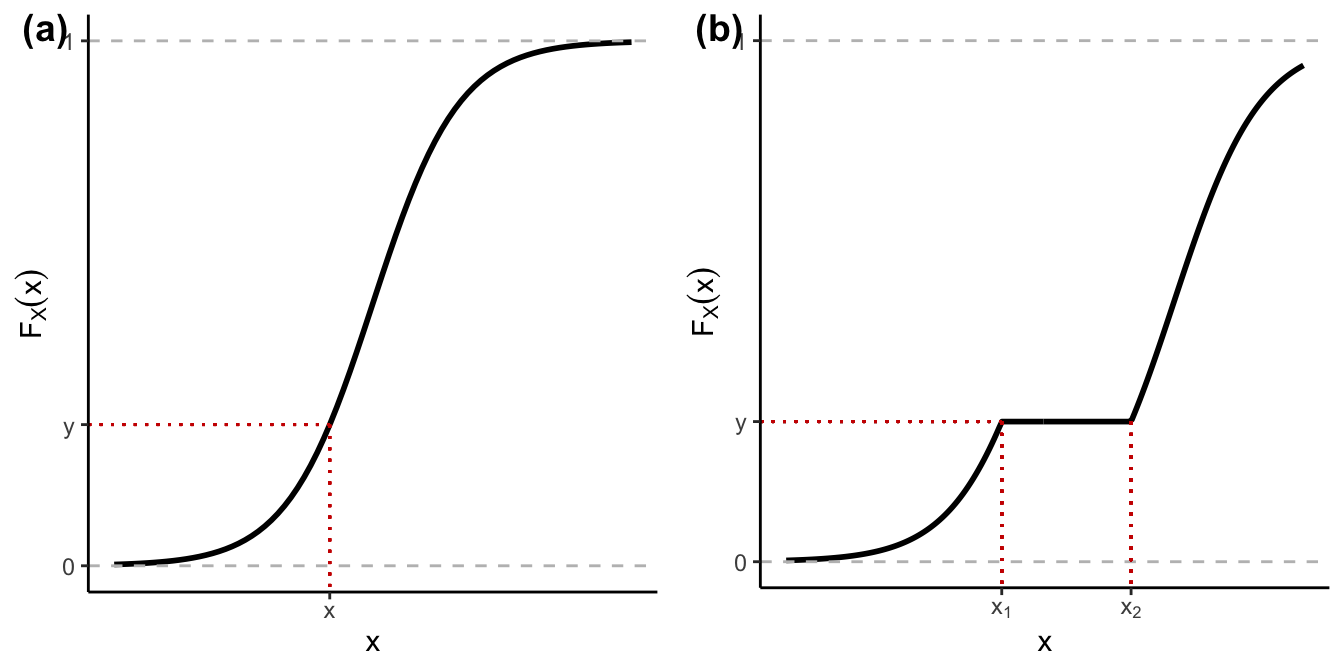
\includegraphics[width=1\linewidth]{bookdown-adv-stats_files/figure-latex/pitflatcdf-1} 

}

\caption{(a) a strictly increasing cdf has a unique inverse; while (b) a non-decreasing cdf has regions in which there is zero probability, so the cdf inverse is the infimum of the \(x\) in that range.}\label{fig:pitflatcdf}
\end{figure}

\end{proof}

The PIT is useful for various statistical purposes, both theoretical and practical.
A particular application of note is the \emph{simulation} of an arbitrary random variable \(X\) on a computer\footnote{Also called \emph{inverse transform sampling}}.

\begin{example}

Let \(X\) be a random variable with an exponential distribution with unit mean.
Its cdf is \(F_X(x) = 1 - e^{-x}\) for \(x>0\).
By the PIT, we have that \(U=1-e^{-X}\) is uniformly distributed on \((0,1)\).

Working a bit backwards, with \(U\sim\Unif(0,1)\) suppose there is (strictly) monotone transformation \(T:[0,1]\to\bbR\) such that \(T(U) := X\). We notice that
\begin{align*}
F_X(x) &= \bbP(X \leq x) \\
&= \bbP\big(T(U) \leq x \big)\\
&= \bbP\big(U \leq T^{-1}(x)\big) \\
&= T^{-1}(x)
\end{align*}
where the last step follows since \(U\) is uniformly distributed on \((0,1)\).
Therefore, \(F_X\) is the inverse function of \(T\), or equivalently \(T(u)=F_X^{-1}(u)\) for \(u\in[0,1]\).
It is then possible to generate \(X\sim\Exp(1)\) using the algorithm below:

\begin{enumerate}
\def\labelenumi{\arabic{enumi}.}
\tightlist
\item
  Generate \(\bU = \{U_1,\dots,U_n\} \sim\Unif(0,1)\).
\item
  Transform the samples \(\bU \mapsto \bX\) using the function \(T(u) = F_X^{-1}(u) = -\log(1-u)\).
\item
  Then \(\bX = \{X_1,\dots,X_n\}\) is a sample from \(\Exp(1)\).
\end{enumerate}

The \texttt{R} code below shows how to implement this in practice. As we can see, the PIT method and the `direct' method using \texttt{R}'s built in function \texttt{rexp()} generates very similar results.

\begin{Shaded}
\begin{Highlighting}[]
\FunctionTok{set.seed}\NormalTok{(}\DecValTok{2911}\NormalTok{)}
\NormalTok{n }\OtherTok{\textless{}{-}} \DecValTok{1000}

\CommentTok{\# Generate Unif(0,1) r.v.}
\NormalTok{U }\OtherTok{\textless{}{-}} \FunctionTok{runif}\NormalTok{(n, }\AttributeTok{min =} \DecValTok{0}\NormalTok{, }\AttributeTok{max =} \DecValTok{1}\NormalTok{) }\SpecialCharTok{\%\textgreater{}\%} \FunctionTok{sort}\NormalTok{()}
\FunctionTok{head}\NormalTok{(U)}
\end{Highlighting}
\end{Shaded}

\begin{verbatim}
## [1] 0.000795529 0.003317551 0.005630351 0.005866332 0.006031142 0.008309819
\end{verbatim}

\begin{Shaded}
\begin{Highlighting}[]
\CommentTok{\# Generate Exp(1) r.v. using PIT}
\NormalTok{X }\OtherTok{\textless{}{-}} \SpecialCharTok{{-}}\FunctionTok{log}\NormalTok{(}\DecValTok{1}\SpecialCharTok{{-}}\NormalTok{U)}
\FunctionTok{head}\NormalTok{(X)}
\end{Highlighting}
\end{Shaded}

\begin{verbatim}
## [1] 0.0007958456 0.0033230660 0.0056462615 0.0058836065 0.0060494031
## [6] 0.0083445376
\end{verbatim}

\begin{Shaded}
\begin{Highlighting}[]
\CommentTok{\# Generate Exp(1) r.v. using R built in function}
\NormalTok{Z }\OtherTok{\textless{}{-}} \FunctionTok{rexp}\NormalTok{(n, }\AttributeTok{rate =} \DecValTok{1}\NormalTok{) }\SpecialCharTok{\%\textgreater{}\%} \FunctionTok{sort}\NormalTok{()}
\FunctionTok{head}\NormalTok{(Z)}
\end{Highlighting}
\end{Shaded}

\begin{verbatim}
## [1] 0.0009589139 0.0020182137 0.0026925327 0.0042910245 0.0043342430
## [6] 0.0045965933
\end{verbatim}

\begin{figure}

{\centering 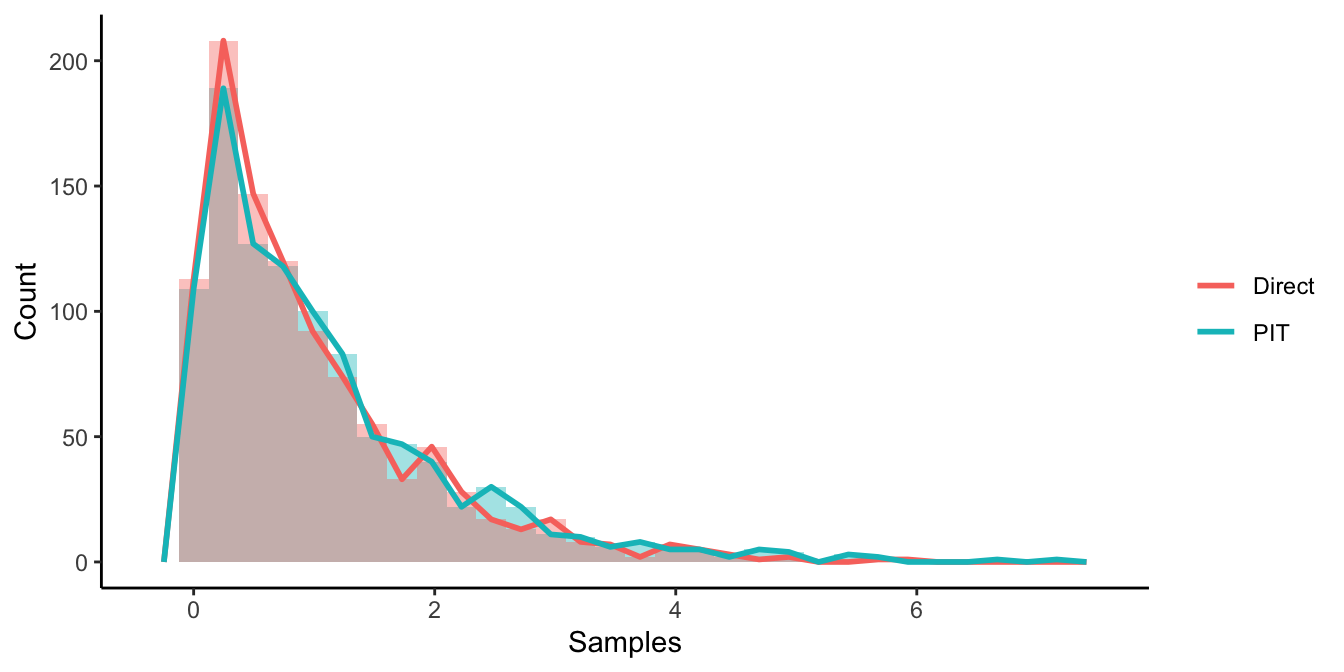
\includegraphics[width=1\linewidth]{bookdown-adv-stats_files/figure-latex/pitexampleplot-1} 

}

\caption{Comparison of histogram and frequency polygon of the samples generated using PIT and the 'direct' method in R.}\label{fig:pitexampleplot}
\end{figure}

\end{example}

\hypertarget{multiple-random-variables}{%
\section{Multiple random variables}\label{multiple-random-variables}}

In the real world, data collection often involves more than one variable, so methods to analyse these kinds of data do exist.
In particular, probability models may well be extended to involve more than one random variable.
These are known as \emph{multivariate models}.

\hypertarget{bivariate-distributions}{%
\subsection{Bivariate distributions}\label{bivariate-distributions}}

Consider the simplest kind, where we deal with only two random variables in each the discrete and continuous case.

\begin{definition}[Joint mass function]
Given a pair of discrete r.v. \(X\) and \(Y\), the joint mass function or joint pmf is defined by
\[
f_{X,Y}(x,y) = \bbP(X=x,Y=y).
\]
\end{definition}

\begin{definition}[Joint density function]
A function \(f_{X,Y}:\bbR^2\to\bbR\) is called a joint probability density function (pdf) of the continuous random vector \((X,Y)\) if for any set \(A\subseteq\bbR^2\),
\[
  \bbP((X,Y) \in A) = \iint_{A} f_{X,Y}(x,y)\dint x \dint y.
\]
\end{definition}

To be clear, bivariate random variables occur in \textbf{pairs}, so that \((X,Y)\) is treated as one entity.
Luckily, all the univariate properties carry over to the bivariate (and even multivariate) case, such as:

\begin{itemize}
\tightlist
\item
  \(f_{X,Y}(x,y) \geq 0\) for all \((x,y) \in \bbR^2\)
\item
  \(\sum_x\sum_y f(x,y) = 1\) if discrete, \(\iint f(x,y)\dint x \dint y = 1\) if continuous
\item
  The joint cdf is defined as
  \begin{align*}
  F_{X,Y}(x,y) &=  \bbP(X\leq x, Y\leq y) \\
  &= \begin{cases}
  \sum_{u\leq x}\sum_{v\leq x} f_{X,Y}(u,v) &\text{discrete case} \\
  \int_{u\leq x}\int_{v\leq x} f_{X,Y}(u,v) \dint u \dint v &\text{continuous case} \\
  \end{cases}
  \end{align*}
\end{itemize}

\begin{example}
A bivariate distribution for two discrete random variable \(X\) and \(Y\) each taking values 0 or 1 can be summarised in the \(2\times 2\) table below.

\begin{longtable}[]{@{}rcc@{}}
\toprule
& \(Y=0\) & \(Y=1\) \\
\midrule
\endhead
\(X=0\) & 1/9 & 2/9 \\
\(X=1\) & 2/9 & 4/9 \\
\bottomrule
\end{longtable}

For instance, \(\bbP(X=1,Y=1) = f(1,1) = 4/9\).

A different way of expressing the above table is by explicitly listing out the probabilities, as follows:
\[
f(x,y) = \begin{cases}
1/9 & x=0,y=0 \\
2/9 & x=0,y=1 \\
2/9 & x=1,y=0 \\
4/9 & x=1,y=1 \\
\end{cases}
\]
\end{example}

\begin{example}
\protect\hypertarget{exm:unitsquare}{}\label{exm:unitsquare}Consider a uniform distribution on the unit square \([0,1] \times [0,1]\). It has pdf given by
\[
f(x,y) = \begin{cases}
  1 &0\leq x \leq 1, 0\leq y \leq 1 \\
  0 &\text{otherwise}
\end{cases}
\]\\
This is a well-defined pdf, as \(f\geq 0\) and \(\int\int f(x,y)\dint x \dint y = 1\).
Suppose we want to find \(\bbP(X<1/2, Y<1/2)\) and \(\bbP(X + Y < 1)\).

For the first probability, we integrate in the set \(\{(x,y) \mid 0 < x <1/2,0< y<1/2\}\):
\begin{align*}
\bbP(X<1/2, Y<1/2) &= \int_0^{1/2} \int_0^{1/2} \dint x \dint y \\
&= \left[ \left[ xy \right]_{0}^{1/2} \right]_{0}^{1/2} = 1/4.
\end{align*}

For the second probability, note that the set \(\{(x,y) \mid x+y<1\}\) corresponds to \(\{(x,y) \mid 0<y<1, 0<x < 1-y\}\). So
\begin{align*}
  \bbP(X+Y<1) &= \int_0^{1} \dint y \int_0^{1-y}  \dint x \\
  &= \int_0^{1} \dint y [x]_0^{1-y} \\
  &= \int_0^{1} (1-y) \dint y = \big[y - y^2/2\big]_0^1 = 1/2.
\end{align*}
\end{example}

Another way of understanding these probabilities is by thinking about them geometrically.
If we plot the pdf surface, it would look something like the following sketch:

\begin{figure}

{\centering 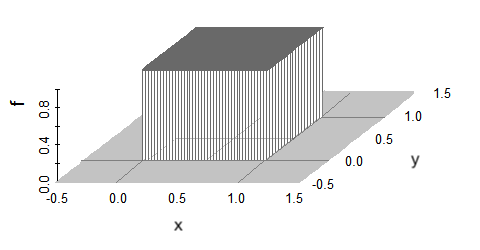
\includegraphics[width=0.8\linewidth]{figure/bivariateunif} 

}

\caption{Pdf surface plot of the uniform distribution on the unit square.}\label{fig:unnamed-chunk-8}
\end{figure}

Any probability of interest would be calculated by finding the volume of interest.
For instance, consider again the probability \(\bbP(X + Y < 1)\).
Viewing the surface from above effectively concentrates on the two dimensions of \(x\) and \(y\).
It's straightforward to realise that the region of interest is anything occuring below the line \(y=x\).

\begin{figure}

{\centering 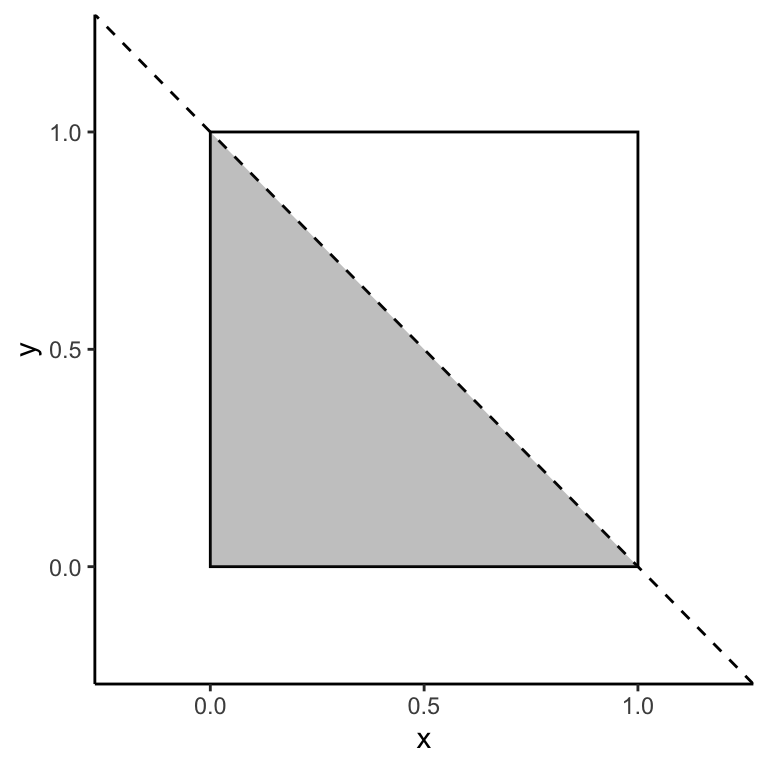
\includegraphics[width=0.6\linewidth]{bookdown-adv-stats_files/figure-latex/bivariateprob-1} 

}

\caption{View of the pdf surface from above, focussing on the X and Y axis.}\label{fig:bivariateprob}
\end{figure}

Correspondingly, we ask what is the volume of this wedge?
It is the area of the shaded region (half of the unit square) multiplied by the height of the surface (1), so we get the same answer of 1/2.

\hypertarget{marginal-distributions}{%
\subsection{Marginal distributions}\label{marginal-distributions}}

We may think of multivariate distributions as several random variables ``stitched'' together, whose distribution as a whole is dependent on each of the components.
Having said this, it is possible recover the distribution for one of the components in a bivariate (or multivariate) model by summing or integrating over the remaining probability distribution, depending on whether or not the other components are discrete or continuous.

\begin{definition}[Marginal distribution]
For a bivariate random variable \((X,Y)\), the marginal distributions of \(X\) and \(Y\) may be obtained respectively as
\[
f_X(x) = 
\begin{cases}
  \sum_y f_{X,Y}(x,y) &\text{if $Y$ is discrete} \\
  \int_y f_{X,Y}(x,y) \dint y &\text{if $Y$ is continuous} \\    
\end{cases}
\]
\[
f_Y(y) = 
\begin{cases}
  \sum_x f_{X,Y}(x,y) &\text{if $X$ is discrete} \\
  \int_x f_{X,Y}(x,y) \dint x &\text{if $X$ is continuous} \\    
\end{cases}
\]
\end{definition}

A note to say that since the joint cdf is defined to be
\[
  F(x,y) = \bbP(X \leq x, Y\leq y),
\]
the \emph{marginal cdfs} can be obtained from the joint cdf for \(X\) by summing over all the components of \(Y\) in the joint cdf, i.e.
\begin{align*}
F_X(x) 
&= \sum_{k\leq x} \left( \sum_y f_{X,Y}(k,y) \right) \\
&= \bbP(X \leq x, Y \leq \infty) \\
&=F_{X,Y}(x,\infty)
\end{align*}
Similarly, we sum up over the components of \(X\) to obtain the marginal cdf for \(Y\), \(F_Y(y)=F_{X,Y}(\infty,y)\).
Note that for continuous random variables, we integrate instead: \(F_X(x) = \int_{-\infty}^x \left(\int f_{X,Y}(\tilde x,y) \dint y \right) \dint \tilde x\).

\begin{example}
Define a joint pdf by
\[
f(x,y) = \begin{cases}
cxy^2 & 0<x<1, 0<y<1\\
0 &\text{otherwise}
\end{cases}
\]
Let's compute the marginal distributions of \(X\) and \(Y\).
We'll have to use integration here since the geometry of the pdf surface in 3-dimensions is a bit complex to work with.

Firstly, we need to find the \emph{normalising constant} \(c\), such that the joint integral of the pdf is 1.
That is, we need to find the value of \(c\) satisfying
\[
\int_{x=0}^1 \int_{y=0}^1 cxy^2 \dint x \dint y = c\left[ \left[ \frac{x^2y^3}{6} \right]_{0}^{1} \right]_{0}^{1} = 1.
\]
We work out that \(c=6\).

To work out the marginal distribution of \(X\), we integrate the pdf over all possible values of \(Y\), i.e.
\begin{align*}
f_X(x) &= \int_{y=0}^1 6xy^2 \dint y \\
&= \left[\frac{6xy^3}{3} \right]_0^1 \\
&= 2x.
\end{align*}
Note that \(f_X(x)=2x\) for \(0<x<1\) is indeed a valid pdf (it integrates to 1, and also satisfies all the properties of a pdf).
We can now use this to calculate probabilities involving only \(X\), for instance
\[
\bbP\left(\frac{1}{2} < X < \frac{3}{4}\right) = \int_{1/2}^{3/4} 2x \dint x = \frac{5}{16}.
\]
\end{example}

\begin{example}
Here's a trickier example.
Consider the joint pdf defined by
\[
f(x,y) = \begin{cases}
e^{-y} & 0<x<y<\infty \\
0 & \text{otherwise.}
\end{cases}
\]
At first glance, it does not seem that the pdf depends on \(x\) at all.
But actually, it does.
If we look at the values at which this pdf is non-zero, it is conditional on the positive values of \(x\) such that it is lesser than \(y\).
To put it more precisely, we could write the pdf as
\[
f(x,y) = \ind_{[\{(u,v) | 0<u<v<\infty\}]}(x,y) e^{-y}
\]
so we can clearly see the dependence of the pdf on both \(x\) and \(y\).
Here, we have used the \emph{indicator function} \(\ind_A(x)\) defined as
\[
\ind_A(x) = \begin{cases}
1 & x\in A \\
0 & x\not\in A.
\end{cases}
\]

To calculate the joint cdf of this bivariate distribution, we compute the integral
\[
F_{X,Y}(x,y) = \int_{u=0}^x \int_{v=u}^y e^{-v} \dint u \dint v 
\]
The limits of integration are obtained as follows: For the random variable \(X\) (using the integrating variable \(u\)) we start at the smallest value it can take (\(u=0\)) and proceed upwards to some arbitrary point \(u=x\). For \(Y\) (using the \(v\) as the variable of integration), the smallest possible value it can take is \(v=u\), since \(x<y<\infty\) and the integration depends on what happens to \(X\). From here, proceed upwards to some arbitrary point \(v=y\).
Working through this integral gives us
\[
F_{X,Y}(x,y) = 1 - (e^{-x}+xe^{-y}), \hspace{2em} 0<x<y<\infty.
\]
This is a valid cdf, since

\begin{itemize}
\tightlist
\item
  \(\lim_{x,y\to 0} F(x,y) = 1-\left(\lim_{x,y\to 0}e^{-x} + \lim_{x,y\to 0} xe^{-y} \right) = 1 - (1 + 0) = 0.\)
\item
  \(\lim_{x,y\to \infty} F(x,y) = 1-\left(\lim_{x,y\to \infty}e^{-x} + \lim_{x,y\to \infty} xe^{-y} \right) = 1 - (0 + 0) = 1.\)
\item
  \(F(x,y)>0\) in that range.
\end{itemize}

From here, the marginal cdf of \(X\) is obtained as \(F_X(x)=F_{X,Y}(x,+\infty)= 1-e^{-x}\) for \(0<x<\infty\).
Noting that the maximum value \(x\) can take is \(y\), we can similarly obtain the marginal cdf of \(Y\) as \(F_Y(y)=F_{X,Y}(+\infty,y) = F(+\infty,y)= F(y,y) = 1-(e^{-y}+ye^{-y})\) for \(0<y<\infty\).
It's easily checked that both of these functions are indeed cdfs.
\end{example}

In the continuous case, the joint cdf of \((X,Y)\) is related to the joint pdf by the relationship
\[
F_{X,Y}(x,y) = \int_{-\infty}^x \int_{-\infty}^y f_{X,Y}(u,v) \dint u \dint v.
\]
By the (bivariate) Fundamental Theorem of Calculus, this implies that
\[
\frac{\partial^2}{\partial x \partial y}F_{X,Y}(x,y) = f_{X,Y}(x,y).
\]

\hypertarget{conditional-distributions}{%
\subsection{Conditional distributions}\label{conditional-distributions}}

Oftentimes when two r.v. \((X,Y)\) are observed, the values of the two variables are ``related''.
What we mean by this is that knowledge about the value of \(Y\) gives us some information about the value of \(X\) and vice versa.
Some examples:

\begin{itemize}
\tightlist
\item
  Height (\(X\)) and weight (\(Y\)) of a person;
\item
  A level points score (\(X\)) and socio-economic status (\(Y\));
\item
  Heart rate (\(X\)) and oxygen saturation levels (\(Y\)).
\end{itemize}

To make this idea a little more concrete, think about what values the heart rate (\(X\)) of an individual can take.
For a healthy individual, this might be anywhere between 40 bpm to 200 bpm (depending on their age, what activity they are doing, and so on).
On average, \(X\) is 72 bpm.
Oxygen saturation levels on the other hand are usually between 95 and 100 percent, but drops below this range when an intense activity is performed.
Consequently, if we were to guess what the heart rate \(X\) value would be given \(Y<0.95\), it would make more sense to guess that \(X=160\) rather than \(X=72\).
This concept should sound familiar!

Define the conditional distributions for discrete and continuous random variables as follows.

\begin{definition}[Conditional distributions, discrete]
If \(X\) and \(Y\) are discrete, the \emph{conditional pmf} of \(X\) given \(Y=y\) is
\[
  f_{X|Y}(x|y) = \bbP(X=x|Y=y) = \frac{\bbP(X=x, Y=y)}{\bbP(Y=y)} = \frac{f_{X,Y}(x, y)}{f_Y(y)},
\]
\end{definition}

\begin{definition}[Conditional distributions, continuous]
If \(X\) and \(Y\) are continuous, the \emph{conditional pdf} of \(X\) given \(Y=y\) is
\[
  f_{X|Y}(x|y) =  \frac{f_{X,Y}(x, y)}{f_Y(y)}.
\]
\end{definition}

In the discrete case, the conditional distribution is derived in a similar way to how the conditional probabilities were (see Definition \ref{def:condprob}).
Interestingly in the continuous case, the definition still looks familiar but it should be noted that plugging \(x\) and \(y\) values into the definition will not yield probabilities--one still requires integration over a set:
\[
\bbP(X \in A|Y=y) = \int_A f_{X|Y}(x|y) \dint x. 
\]

Note that as a function of \(x\), \(f_{X|Y}(x|y)\) is indeed a pdf, since in the discrete case
\[
\sum_x f_{X|Y}(x|y) = \sum_x \frac{\bbP(X=x, Y=y)}{\bbP(Y=y)} = \frac{\bbP(Y=y)}{\bbP(Y=y)} = 1,
\]
and in the continuous case,
\[
\int f_{X|Y}(x|y) \dint x = \int \frac{f_{X,Y}(x, y)}{f_Y(y)} \dint x = \frac{f_Y(y)}{f_Y(y)} = 1.
\]

Finally, it's convenient to note that, just like as we saw for conditional probabilities, we can rearrange the equations to yield \[f_{X|Y}(x|y)f_Y(y)=f_{Y|X}(y|x)f_X(x).\]

\begin{example}
Let \(X\) and \(Y\) have the joint pdf \(f(x,y)=x+y\) for \(0\leq x,y\leq 1\).
Suppose \(Y=a\) has been observed, where \(a\in[0,1]\).
Firstly, the the pdf of \(Y\) is
\[
f_Y(y) = \int_0^1 (x+y) \dint x = \left[xy +y^2/2\right]_0^1 = y + 1/2.
\]

The conditional pdf for \(X\) is
\[
f_{X|Y}(x|Y=a) = \frac{f_{X,Y}(x,Y=a)}{f_Y(a)} = \frac{x+a}{a + 1/2}.
\]

We can compute \(\bbP(X<1/4|Y=1/3)\) by
\begin{align*}
\bbP(X<1/4|Y=1/3) = (1/3 + 1/2)^{-1} \int_{0}^{1/4} (x+1/3) \dint x = 11/80.
\end{align*}
\end{example}

It is possible to also describe \emph{conditional cdfs}.
If we treat the conditional pmf/pdf \(f(x|y)\) as a new pmf/pdf \(g(x)\), then the cdf can be easily obtained in the usual way: \(F(x|y)=G(x)=\bbP(X\in A|y)\).

\hypertarget{independent-random-variables}{%
\subsection{Independent random variables}\label{independent-random-variables}}

Previously we came across the concept of independence of probabilistic events.
We can extend this notion to random variables using the conditional pmf/pdf definitions.

\begin{definition}[Independece of r.v.]
Two random variables \(X\) and \(Y\) are independent if and only if for every \(x\in\bbR\) and \(y\in\bbR\),
\[
  f_{X,Y}(x,y) = f_X(x)f_Y(y).
\]
We write \(X \perp Y\).
\end{definition}

Apparently, if there exists functions \(g(x)\) and \(h(y)\) (not necessarily pdfs) such that \(f(x,y)=g(x)h(y)\) for all \(x,y\), then \(X\) and \(Y\) are independent.
This is proven in Lemma 4.2.7 of C\&B.
Hence, verifying whether two random variables are independent is made easier, since we only need to separate out the components of \(x\) and \(y\) in the joint pdf without needing to check whether or not the components themselves are pdfs.

The assumption of independence is used very often in statistical inference as it simplifies calculations quite a lot.
We'll circle back to this thought when we talk about likelihood estimation.

\begin{example}
Recall the bivariate distribution on the unit square (c.f. Example \ref{exm:unitsquare}).
Note that the pdf of \(X\) is \(f_X(x) = \int_0^1 \dint y = 1\), and similarly \(f_Y(y)=1\).
It is easy to see that \(X\) and \(Y\) are independent, since
\[
f_{X,Y}(x,y) = 1 = f_X(x)f_Y(y).
\]
As a consequence, to generate a random sample from \((X,Y)\), one can randomly sample values \(X\sim\Unif(0,1)\), and independently sample \(Y\sim\Unif(0,1)\).
\end{example}

\hypertarget{expectations}{%
\section{Expectations}\label{expectations}}

The expected value, or expectation, of a random variable \(X\) is its average value \emph{weighted} according to the probability distribution.
Simply put, it signifies the \emph{arithmetic mean} of a large number of independent realisations of \(X\).

\begin{definition}[Expectation]
The \emph{expected value} or \emph{mean} of a random variable \(X\), denoted \(\E(X)\), is defined to be
\[
\E(X) = \begin{cases}
  \sum_x x f_X(x) = \sum_x x \bbP(X=x) &\text{if $X$ is discrete} \\
  \int x f_X(x) \dint x &\text{if $X$ is continuous} \\  
\end{cases}
\]
provided that the integral or sum exists (is finite).
\end{definition}

The symbol `\(\mu\)' is often used to denote the expected value. It may be represented by \(\E X\), \(\E[X]\) or even using \(\bbE\) instead of \(\E\).

The expectation of a random variable is \textbf{not to be confused} with the \emph{sample mean} of a set of observations \(\{x_1,\dots,x_n \}\), i.e.~\(\bar x_n = \frac{1}{n} \sum_{i=1}^n x_i\).
The expectation is a purely theoretical value based on probabilities and pdfs.
The sample mean incorporates \emph{randomness} into the calculations, by virtue of the randomness of the observed set of sample values.

\begin{example}
Let \(X \in \{0,1\}\) take value 1 with probability \(p\), and 0 with probability \(1-p\).
\(X\) is called a Bernoulli random variable, and we write \(X \sim \Bern(p)\).
Then,

\[
\E(X) = \sum_x x\bbP(X = x) = 1\cdot p + 0 \cdot (1-p) = p.
\]
\end{example}

\begin{example}
Let \(X\) be a continuous random variable with pdf \(f(x)=\frac{1}{b-a}\), where \(a,b\in\bbR\) and \(a<b\).
\(X\) has what is called a uniform distribution on the interval \((a,b)\), and we write \(X\sim\Unif(a,b)\). The mean of \(X\) is

\[
\E(X) = \int_a^b  \frac{x}{b-a} = \frac{a+b}{2},
\]

the midpoint of the interval \((a,b)\)! This reveals some intuition regarding uniformity of the distribution.
\end{example}

Do all random variables have expectations?

\begin{example}

\begin{center}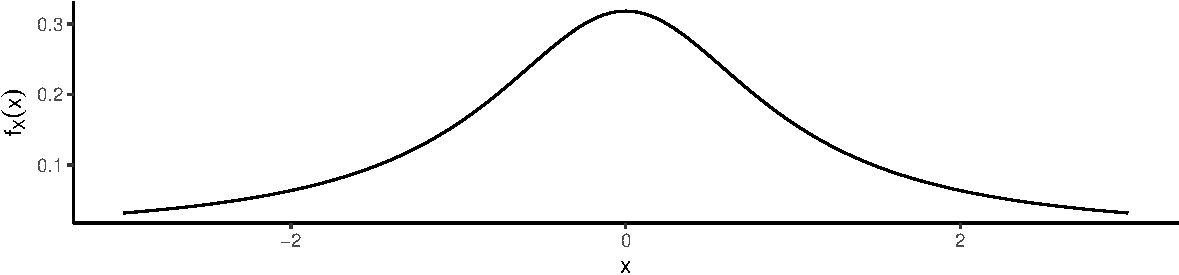
\includegraphics[width=1\linewidth]{bookdown-adv-stats_files/figure-latex/cauchy-1} \end{center}

Let \(X\) be a continuous random variable with pdf \(f(x)=\{ \pi(1+x^2) \}^{-1}\) with support over \(\bbR\).
This is the Cauchy distribution\footnote{Named after the French mathematician Augustin Cauchy, although in physics, it is often known by the Lorentz distribution after the Dutch Nobel Laureate Hendrik Lorentz.} with location and scale parameter 0 and 1 respectively.
Let's calculate the mean.

Using the substitution \(u = x^2 + 1\) and \(\dint u/2 = x \dint x\), we find that
\begin{align*}
\E(X) 
&= \int_{-\infty}^\infty \frac{x \dint x}{\pi(1+x^2)} \\
&= \int_{-\infty}^0 \frac{x \dint x}{\pi(1+x^2)} + \int_{0}^\infty \frac{x \dint x}{\pi(1+x^2)} \\
&= \frac{1}{2\pi} \int_{u=\infty}^{u=1} \frac{\dint u}{u} + \frac{1}{2\pi} \int_{u=1}^{u=\infty} \frac{\dint u}{u} \\
&= \frac{1}{2\pi} \left[\log u \right]_{\infty}^{1} + \frac{1}{2\pi} \left[\log u \right]^{\infty}_{1} \\
&= \frac{1}{2\pi} (\infty - \infty) = \ ???
\end{align*}

The mean of the Cauchy distribution is undefined.
This seems a bit weird, since we can see that the pdf is somewhat bell-shaped with its peak at 0, so wouldn't we expect the mean to be zero?
Not quite.
The highest peak of the bell curve is known as the \emph{mode} of the distribution, and that indeed is well defined and is zero.
The \emph{median} is also well-defined, as this is the point at which half the distribution lies below, and half lies above it--the median is zero.
The median exists because the area under the pdf curve must necessarily be equal to 1, a finite value.

On the other hand, if we look at the plot of \(xf(x)\) on the positive side of the real line, we see that the tail end does not drop fast enough for the area under the curve to be a finite number.

\begin{center}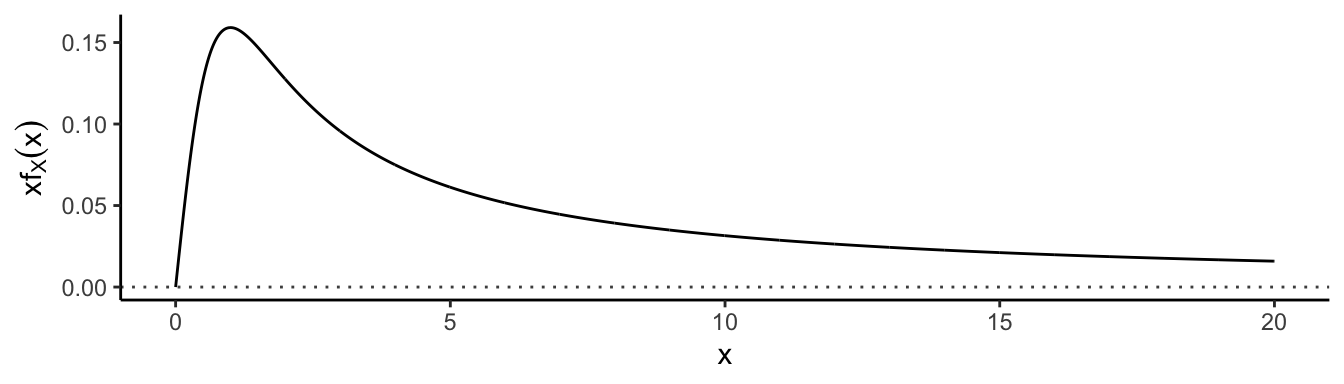
\includegraphics[width=1\linewidth]{bookdown-adv-stats_files/figure-latex/cauchy2-1} \end{center}

\end{example}

\hypertarget{expectations-of-functions-of-r.v.}{%
\subsection{Expectations of functions of r.v.}\label{expectations-of-functions-of-r.v.}}

Realise that if \(X\) is a r.v., then any function of \(X\), \(g(X)\), is also a random variable\footnote{We can even describe the distribution for any transformation of \(X\), see C\&B Sec 2.1.}.
Often time we will want to know the mean of \(g(X)\).

\begin{theorem}
Let \(X\) be a r.v. with pdf \(f_X(x)\), and let \(Y=g(X)\). Then
\[
\E(Y) = \int g(x)f_X(x)\dint x.
\]
\end{theorem}

In particular, the \(k\)th \textbf{moment} of \(X\) for \(k\in\bbZ\) is defined to be
\[
\E(X^k) = \int x^kf_X(x)\dint x.
\]
The \(k\)th central moment is defined as \(\E((X-\mu)^k)\), where \(\mu:=\E(X)\).

\hypertarget{properties-of-expectations}{%
\subsection{Properties of expectations}\label{properties-of-expectations}}

Let \(X\) be a r.v., and \(a,b,c\in\bbR\) be constants.
Here are some important properties of expectations.

\begin{itemize}
\tightlist
\item
  \(\E(aX +bX +c) = a\E(X) + b\E(X) + c\) (linearity of expectations)
\item
  If \(Y\) is a r.v. s.t. \(X\perp Y\), then \(\E(XY) = \E(X)\E(Y)\)
\item
  If \(X\geq 0\) for all \(x\), then \(\E(X)\geq 0\)
\item
  If \(a \leq X \leq b\) for all \(x\), then \(a \leq \E(X) \leq b\)
\item
  \(\E(X) = \min_b \E((X-b)^2)\)\footnote{See Example 2.2.6 C\&B.}
\end{itemize}

Note that the above properties work for any transformations of \(X\) too.
For instance, \(\E(ag(X) +bg(X) +c) = a\E(g(X)) + b\E(g(X)) + c\). Just think of \(Y=g(X)\) as a new random variable.

If \(X\) and \(Y\) are \uline{not} independent, then \(\E(XY) \neq \E(X)\E(Y)\).

The last property above implies that the mean of a random variable is the minimiser of the (expected) quadratic loss function:
The closer \(b\) is to \(X\), then the smaller the value of \((X-b)^2\).
We can also ask what is the expected value of \(b\) which minimises this quantity, and the answer is the mean of \(X\).
The interpretation here is that \(\E(X)\) is a good guess of the value of \(X\)! At least, as measured by this quadratic loss function.

As a corollary to the linearity property, if \(X_1,\dots,X_n\) are r.v. and \(a_1,\dots,a_n\) are constants, then
\[
\E\left(\sum_{i=1}^n a_iX_i \right) = \sum_{i=1}^n a_i\E(X_i).
\]
Additionally, if \(X_1,\dots,X_n\) are \textbf{independent},
\[
\E\left(\prod_{i=1}^n a_iX_i \right) = \prod_{i=1}^n \E(X_i).
\]

These properties are used extensively throughout statistics, so please take the time to memorise and learn these.
It will make tackling questions in the later chapter much easier!

\hypertarget{variance}{%
\subsection{Variance}\label{variance}}

Aside from the mean of a random variable (its first central moment), another important concept is the second central moment, more commonly known as the variance.

\begin{definition}[Variance]
Let \(X\) be a r.v. with mean \(\mu\). The \emph{variance} of \(X\) is defined
\[
\Var(X) = \E\big[(X-\mu)^2\big],
\]
assuming this expectation exists. The \emph{standard deviation} is \(\text{sd}(X) = \sqrt{\Var(X)}\).
\end{definition}

The symbol \(\sigma^2\) is often used to denote the variance, and \(\sigma\) the standard deviation.
An alternative (and arguably easier) formula for the variance is \[\sigma^2 = \E(X^2) - \{\E(X)\}^2\].
But take caution, that this formula can be less precise than the one given in the definition above.
Especially when \(X\) takes very large (or very small) values, then correspondingly \(\E(X^2)\) and \(\E(X)\) will be very large (very small) too.
Computationally, there is a limited number of integers the computer can store (its single-precision floating point), and once this is exceeded the numbers get less precise.
On the other hand, the formula in the definition avoids this issue because the difference between \(X\) and its mean is ``tamed'' in a way--the expected value is zero!

This variance is \textbf{not to be confused} with the *sample variance() of a set of observations \(\{x_1,\dots,x_n\}\), i.e.~\(s^2 = \frac{1}{n}\sum_{i=1}^n (x_i-\bar x_n)^2\). However, do inspect the two formulae for similarities!

The variance measures the spread of a distribution, that is, how far apart or close together the ``mass'' of a distribution are.
To illustrate this, have a look at the following \(\N(0,\sigma^2)\) pdfs for different values of \(\sigma^2\).

\begin{center}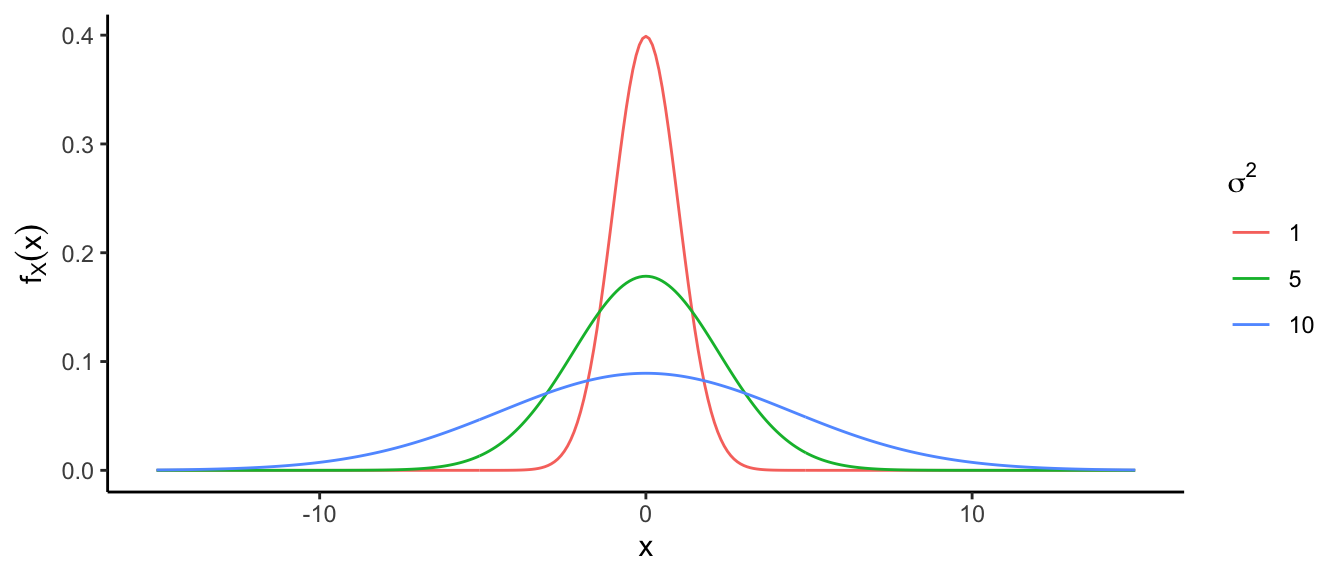
\includegraphics[width=1\linewidth]{bookdown-adv-stats_files/figure-latex/normaldist-1} \end{center}

Larger values of \(\sigma\) indicate a wider spread (away from the mean), and conversely, smaller values indicate a smaller spread, where values are close together near the mean.
The variance will become an important criterion when determining how good or bad an parameter estimator is.
More on this in Chapter 4!

\hypertarget{covariance-and-correlation}{%
\subsection{Covariance and correlation}\label{covariance-and-correlation}}

Suppose we had two random variables, and we wanted to see how each random variable behaves in their respective domains, but also together.
That is, are larger values of \(X\) associated with larger or smaller values of \(X\), or is there no relationship at all?
We introduce the concept of covariance and correlation, both of which measure how strong the \emph{linear relationship} is between \(X\) and \(Y\).

\begin{definition}[Covariance]
For two random variables \(X\) and \(Y\) with finite means \(\mu_X\) and \(\mu_Y\) respectively, the covariance between \(X\) and \(Y\) is

\[
\Cov(X,Y) = \E\big[(X-\mu_X)(Y-\mu_Y) \big],
\]
assuming this expectation exists.
If the variances of the two random variables are finite, then the covariance between them exists.
\end{definition}

As with the variance formula, there is also an alternative formula for the covariance given by \[\Cov(X,Y) = \E(XY) -\E(X)\E(Y).\]
This formula is also susceptible to catastrophic cancellation, and should be avoided in computer programs\footnote{See this article: \url{https://en.wikipedia.org/wiki/Covariance\#Numerical_computation}}.
Note that the covariance of \(X\) with itself is \(\sigma^2\), which can be seen by plugging in \(X\) for \(Y\) in the formula above.

The magnitude of the covariance by itself does not reflect how strong the relationship between \(X\) and \(Y\) is, so this is where correlation comes in.

\begin{definition}[Correlation]
For two r.v. \(X\) and \(Y\) with finite means \(\mu_X\) and \(\mu_Y\) resp., and variances \(\sigma^2_X\) and \(\sigma^2_Y\) resp., the correlation between \(X\) and \(Y\) is the number \(\rho\in[-1,1]\) defined by

\[
\rho_{XY} :=  \frac{\Cov(X,Y)}{\sigma_X\sigma_Y}
\]
\end{definition}

The value \(\rho_{XY}=0\) implies that there is no linear relationship at all between \(X\) and \(Y\).
On the other hand, \(\rho_{XY}=1\) (\(\rho_{XY}=-1\)) implies a perfect positive (negative) linear relationship.
In fact, \(|\rho_{XY}=1|\) if and only if \(\exists a\neq 0,b\in\bbR\) such that \(\bbP(Y=aX+b)=1\).
If \(a>0\) then \(\rho_{XY}=1\), and if \(a<0\) then \(\rho_{XY}=-1\).

The relationship between covariance/correlation with independence is the following: If \(X\) and \(Y\) are independent, then \(\Cov(X,Y) =\rho_{XY}=0\). This can easily be proven using properties of expectations.

The converse however is not true!
If \(\Cov(X,Y)=\rho_{XY}=0\), then \(X\) and \(Y\) are \textbf{not necessarily} independent.
The reverse statement is true for normal random variables, but not in general.
This is one of the properties of normal distributions which we'll cover in the next chapter.

What does \emph{linear} relationship mean?
As the name implies, a strong covariance/correlation allows us to draw a straight line through the points plotted in a 2-dimensional scatterplot.
Let's take a look.

Let \(X,Y\iid\N(0,1)\).
We can draw some random values in \texttt{R}, and produce a scatterplot to see the relationship between them.

\begin{Shaded}
\begin{Highlighting}[]
\FunctionTok{set.seed}\NormalTok{(}\DecValTok{789}\NormalTok{)}
\NormalTok{X }\OtherTok{\textless{}{-}} \FunctionTok{rnorm}\NormalTok{(}\AttributeTok{n =} \DecValTok{100}\NormalTok{, }\AttributeTok{mean =} \DecValTok{0}\NormalTok{, }\AttributeTok{sd =} \DecValTok{1}\NormalTok{)}
\NormalTok{Y }\OtherTok{\textless{}{-}} \FunctionTok{rnorm}\NormalTok{(}\AttributeTok{n =} \DecValTok{100}\NormalTok{, }\AttributeTok{mean =} \DecValTok{0}\NormalTok{, }\AttributeTok{sd =} \DecValTok{1}\NormalTok{)}
\FunctionTok{qplot}\NormalTok{(X, Y, }\AttributeTok{geom =} \StringTok{"point"}\NormalTok{)}
\end{Highlighting}
\end{Shaded}

\begin{center}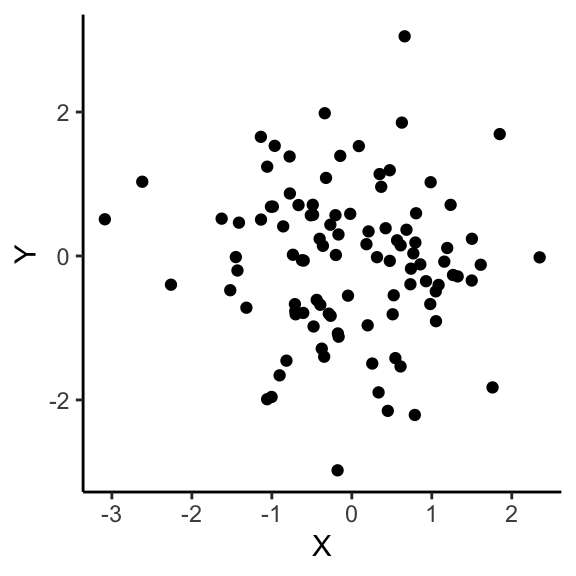
\includegraphics[width=0.6\linewidth]{bookdown-adv-stats_files/figure-latex/corr1-1} \end{center}

Since the objects \texttt{X} and \texttt{Y} are drawn separately, they are independent of each other.
If we were to draw a straight line through the data points above, how would we draw such a line?
There does not seem to be a ``right'' way of doing it.
This illustrates the concept of zero correlation.

Now suppose \(Y=2X + Z\), where \(Z\sim\N(0,1)\).
Now, \(\Cov(X,Y)= 2\), and \(\Var(Y)=2\)--try and work this out yourself!
Theoretically, \(\rho_{XY}=2/\sqrt{1\cdot 2}\approx 0.71\).

\begin{Shaded}
\begin{Highlighting}[]
\NormalTok{Z }\OtherTok{\textless{}{-}} \FunctionTok{rnorm}\NormalTok{(}\AttributeTok{n =} \DecValTok{100}\NormalTok{, }\AttributeTok{mean =} \DecValTok{0}\NormalTok{, }\AttributeTok{sd =} \DecValTok{1}\NormalTok{)}
\NormalTok{Y }\OtherTok{\textless{}{-}} \DecValTok{2} \SpecialCharTok{*}\NormalTok{ X }\SpecialCharTok{+}\NormalTok{ Z}
\FunctionTok{cor}\NormalTok{(X, Y)  }\CommentTok{\# calculate sample correlation}
\end{Highlighting}
\end{Shaded}

\begin{verbatim}
## [1] 0.9018487
\end{verbatim}

\begin{Shaded}
\begin{Highlighting}[]
\FunctionTok{qplot}\NormalTok{(X, Y, }\AttributeTok{geom =} \StringTok{"point"}\NormalTok{)}
\end{Highlighting}
\end{Shaded}

\begin{center}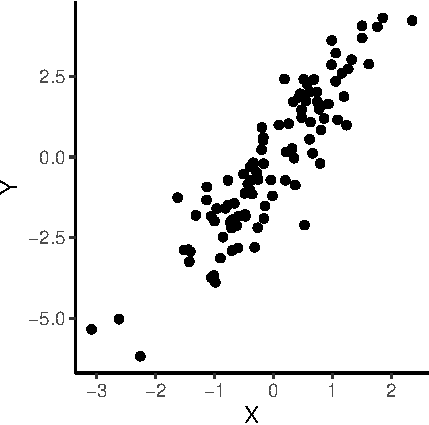
\includegraphics[width=0.6\linewidth]{bookdown-adv-stats_files/figure-latex/corr2-1} \end{center}

As the two random variables are positively correlated, a pattern emerges in the scatterplot, where it seems natural to draw a straight line between the points.
Positive correlation suggests that higher values of \(X\) are associated with higher values of \(Y\), and vice versa.

\hypertarget{properties-of-variances-and-covariances}{%
\subsection{Properties of variances and covariances}\label{properties-of-variances-and-covariances}}

In this section, we shall state some properties of variances and covariances without proof.
You may work this out for yourself, or refer to the textbooks for proofs.
While the properties for variance and covariances look similar, there are subtle differences between them.
Make sure you note these differences, and study them properly, and preferably commit them to memory so we can make use of these in later calculations.

Let \(X\) and \(Y\) be random variables, and \(a\neq0,b\in\bbR\) be constants.

\begin{itemize}
\tightlist
\item
  \(\Var(aX + b) = a^2\Var(X)\)
\item
  \(\Var(X \pm Y) = \Var(X) + \Var(Y) \pm 2\Cov(X,Y)\)
\item
  If \(X\) and \(Y\) are independent, then \(\Var(X \pm Y) = \Var(X) + \Var(Y)\)
\end{itemize}

As a corollary, let \(X_1,\dots,X_n\) be r.v. Then,
\[
\Var \left(\sum_{i=1}^nX_i \right) = \sum_{i=1}^n \Var(X_i) + \sum_{i\neq j}\Cov(X_i,X_j)
\]

Let \(X,Y,W,V\) be r.v., and \(a,b,c,d\in\bbR\). Then

\begin{itemize}
\tightlist
\item
  \(\Cov(X,Y) = \Cov(Y,X)\)
\item
  \(\Cov(X,b) = 0\)
\item
  \(\Cov(aX,Y) = a\Cov(X,Y)\)
\item
  \(\Cov(aX+b,cY+d)=ac\Cov(X,Y)\)
\item
  \(\Cov(X+Y,W+V)=\Cov(X,Y) + \Cov(X, V) + \Cov(Y,W) + \Cov(Y,V)\)
\end{itemize}

\begin{example}
Let \(X\sim\N(0,1)\), and \(Y=2X+1\). Then \[\Var(Y)=\Var(2X+1)=4\Var(X) = 4.\] Further, \[\Cov(X,Y)=\Cov(X,2X+1)=2\Cov(X,X)=2\Var(X)=2.\]
\end{example}

\hypertarget{multivariate-means-and-covariances}{%
\subsection{Multivariate means and covariances}\label{multivariate-means-and-covariances}}

In the previous section, we discussed bivariate and multivariate random variables.
Let's take a look briefly at how one would define expectations and variances for these types of variables.
We'll study the more general \(p\)-dimensional random variable, and hopefully you'll be able to interpolate to bivariate cases yourself.

Consider a random vector \(\bX = (X_1,\dots,X_p)^\top\) with pdf given by \(f_{\bX}(\bx)\) and support over \(\bbR^p\).
We define the mean of this random vector as the component-wise mean of the random variables.

\begin{definition}[Mean vector]
Let \(\bX\in\bbR^p\) be a random vector as described. The \emph{mean vector} of \(\bX\) is
\[
\bmu = (\mu_1,\dots,\mu_p)^\top,
\]
where each \(\mu_k\) is the mean of each component of the random vector, i.e.
\[
\mu_k = \E(X_k) = \begin{cases}
\sum_x x\bbP(X_k=x) & \text{discrete case} \\
\int_x xf_{X_k}(x) \dint x & \text{continuous case} \\
\end{cases}
\]
This is assuming that each of these mean components \(\mu_k\) are finite.
\end{definition}

In order to calculate the mean vector from scratch, we need the marginal distributions of each of the components of \(\bX\).

In a similar manner we may define the \emph{variance-covariance} matrix.
That is, we compute each of the variance of the components of the random vector and collect them into a matrix.
Additionally, we have to compute each pairwise covariance to complete populating the matrix.

\begin{definition}[Variance-covariance matrix]
Let \(\bX\in\bbR^p\) be a random vector as described. The \emph{variance-covariance matrix} of \(\bX\) is the \(p \times p\) square, symmetric matrix \(\bSigma=(\sigma_{ij})\) where each entry is defined by
\begin{align*}
\sigma_{ij} 
&= \E\big[(X_i-\mu_i)(X_j-\mu_j) \big] 
\end{align*}
for all \(i,j=1,\dots,p\).
\end{definition}

Realise that to compute the variance-covariance matrix, one requires the pairwise joint pdfs of the components of \(\bX\).
For illustration, we can see that the \(\bSigma\) matrix looks something like this:

\[
\bSigma = \begin{pmatrix}
\Var(X_1)   &\Cov(X_1,X_2) &\cdots &\Cov(X_1,X_p) \\
\Cov(X_2,X_1)   &\Var(X_2) &\cdots &\Cov(X_2,X_p) \\
\vdots &\vdots &\ddots&\vdots \\
\Cov(X_p,X_1)   &\Cov(X_p,X_2) &\cdots &\Var(X_p) \\
\end{pmatrix}
\]

The \(p\) diagonal entries of \(\bSigma\) are the variances of each \(X_k\), which there are \(p\) of them.
The off-diagonal entries are the covariances.
It is symmetric because \(\Cov(X_i,X_j)=\Cov(X_j,X_i)\).

The correlation matrix is similar in structure to the above, with the difference that each entry in the matrix is
\[
\sigma_{ij} = \frac{\E\big[(X_i-\mu_i)(X_j-\mu_j) \big]}{\sigma_i\sigma_j} = \rho_{X_iX_j},
\]
where \(\sigma_k\) is the standard deviation of each of the components \(X_k\).
As a result, the correlation matrix has all diagonals equal to 1, and the off-diagonals represent the correlations between the random variables.

An important type of correlation matrix is the identity matrix \(\bI_p\), where all the diagonals are 1 and the off-diagonals are 0.
As we discussed, this does not necessarily imply that the components of \(\bX\) are independent.
However, in the special case of the (multivariate) normal distribution, the identity matrix correlation matrix implies \(p\) independent unit variance normal variates.

\begin{example}
Here we'll look at a bivariate random variable \(\bX=(X_1,X_2)^\top\in[0,1]^2\), whose pdf is given by
\[
f_{X_1,X_2}(x_1,x_2) = \frac{1}{2} + \frac{3}{4}(x_1^2 + x_2^2).
\]
The pdf can be visualised as follows.

\begin{verbatim}
## 
## Attaching package: 'plotly'
\end{verbatim}

\begin{verbatim}
## The following object is masked from 'package:ggplot2':
## 
##     last_plot
\end{verbatim}

\begin{verbatim}
## The following object is masked from 'package:stats':
## 
##     filter
\end{verbatim}

\begin{verbatim}
## The following object is masked from 'package:graphics':
## 
##     layout
\end{verbatim}

Let's compute the means and variances of each components \(X_1\) and \(X_2\). For this, we need the marginal pdfs.
\[
f_{X_1}(x) = \int_{0}^1 \left(\frac{1}{2} + \frac{3}{4}(x^2 + y^2) \right) \dint y = \frac{3}{4}(x^2 + 1)
\]
and by symmetry,
\[
f_{X_2}(x) = \frac{3}{4}(x^2 + 1).
\]
Both of these pdfs are valid, since they both integrate to 1 in the unit interval region of integration.
Since they are identically distributed, \(\E(X_1)=\E(X_2)\) and \(\Var(X_1)=\Var(X_2)\).
We compute these in turn.

\begin{align*}
\E(X_1) &= \int_0^1 x\frac{3}{4}(x^2 + 1) \dint x = \frac{9}{16} = \E(X_2),
\end{align*}
and
\begin{align*}
\Var(X_1) &= \int_0^1 \left(x - \frac{9}{16}\right)^2 \frac{3}{4}(x^2 + 1) \dint x = 0.0836 = \Var(X_2).
\end{align*}

As for the covariance, this is computed as follows.
\begin{align*}
\Cov(X_1,X_2) &= \int_0^1 \int_0^1 \left(x - \frac{9}{16}\right)\left(y - \frac{9}{16}\right) \left( \frac{1}{2} + \frac{3}{4}(x^2 + y^2) \right) \dint x \dint y \\
&= -0.00391
\end{align*}

Therefore, the mean vector for \((X,Y)\) is
\[
\bmu = \begin{pmatrix}
\mu_1\\
\mu_2
\end{pmatrix}
=
\begin{pmatrix}
9/16 \\
9/16
\end{pmatrix}
\]
while the variance-covariance matrix is
\[
\bSigma = \begin{pmatrix}
\Var(X_1) & \Cov(X_1,X_2) \\
\Cov(X_1,X_2) & \Var(X_2) \\
\end{pmatrix} 
=
\begin{pmatrix}
0.0836 & -0.00391 \\
-0.00391 & 0.0836 \\
\end{pmatrix}.
\]
If we were to convert the above \(2\times 2\) matrix to a correlation matrix, we would need to divide each entry by \(\sqrt{\Var(X_1)\Var(X_2)}=0.0836\), thus yielding the correlation matrix \(\bPhi\)
\[
\bPhi = \begin{pmatrix}
1 & \rho(X_1,X_2) \\
\rho(X_1,X_2) & 1 \\
\end{pmatrix} 
=
\begin{pmatrix}
1 & -0.05 \\
-0.05 & 1 \\
\end{pmatrix}.
\]
\end{example}

\hypertarget{conditional-expectations-and-variance}{%
\subsection{Conditional expectations and variance}\label{conditional-expectations-and-variance}}

In the previous section, we looked at conditional probability functions, both in the discrete and continuous case.
These conditional pmfs/pdfs are also useful for calculating \emph{conditional expectations}, i.e.~the ``average'' value of a random variable \(X\) given some information about another random variable \(Y\) which might affect it.
We define it as follows.

\begin{definition}[Conditional expectation]
The \emph{conditional expectation} of a function of a random variable \(X\), \(g(X)\) say, given a value of another random variable \(Y=y\), is
\[
\E\left[g(X)|Y=y\right] =
\begin{cases}
\sum_x g(x)\overbrace{\bbP(X=x|Y=y)}^{f_{X|Y}(x|y)} &\text{if $X$ is discrete}\\
\int g(x)f_{X|Y}(x|y)\dint x &\text{if $X$ is continuous}\\
\end{cases}
\]
\end{definition}

In particular, we might be interested in \(\E(X|Y)\), which is obtained using \(g(X)=X\) in the above definition.
Notice that to calculate the conditional expectations, we require the conditional distributions.

Conditional expectations behave quite like regular expectations, so that all of the properties of the usual expectations are applicable.
However, whereas \(\E(X)\) is a number (non-random), \(\E(X|Y=y)\) is a function of \(y\).
More importantly, if we have \uline{not observed} \(Y\), then \(\E(X|Y)\) is a \textbf{random variable}.

There are some additional properties related to conditional expectations that are somewhat intuitive.
We list them here for reference.

\begin{itemize}
\item
  \(\E(g(X) | X) = g(X)\)--``the given variable is a constant''
\item
  \(\E(g(X) Y | X) = g(X) \E(Y|X)\)--since \(g(X)\) given \(X\) is a constant, we can pull it out of the expectation.
\item
  If \(X \perp Y\), then \(\E(Y|X)=\E(Y)\)--since the distribution of \(Y\) does not depend on \(X\).
\end{itemize}

Let's take a look at an example.

\begin{example}
Suppose we draw \(Y\sim\Unif(0,1)\).
After we observe \(Y=y\in[0,1]\), we draw \(X|(Y=y) \sim \Unif(y,1)\).
That is, conditional on the observed value of \(Y\), we draw another uniform distribution whose value is at least \(Y\) and at most \(1\).
Intuitively, since this is a uniform distribution, we expect that \(\E(X|Y=y)\) to be half-way between \(y\) and 1, i.e.~\((1+y)/2\).

In fact this is indeed the case, since \(f_{X|Y}(x|y) = (1-y)^{-1}\), so
\begin{align*}
\E(X|Y=y) 
&= \int_y^1 xf_{X|Y}(x|y) \dint x \\ 
&= \frac{1}{1-y} \int_y^1  x \dint x  \\
&=\frac{1-y^2}{2(1-y)} \\
&= \frac{(1-y)(1+y)}{2(1-y)} \\
&=\frac{1+y}{2}.
\end{align*}

However, if \(Y\) has not been observed yet, then \(\E(X|Y)=(1+Y)/2\) is a random variable whose value is \(\E(X|Y=y)=(1+y)/2\) once observed.
\end{example}

If \(\E(X|Y)\) is a random variable, then it must have a distribution.
Sometimes this is easy to figure out, but other times it is not so straightforward.
However, we have a result to easily obtain the mean of this random variable \(\E(X|Y)\).

\begin{theorem}[Rule of iterated expectations/Law of total expectations]
\protect\hypertarget{thm:lawoftotalexp}{}\label{thm:lawoftotalexp}If \(X\) and \(Y\) are two random variables, then
\[
{\E}_Y\left[\E(X|Y)\right] = \E(X),
\]
provided the expectation exists.
More generally, \(\E(g(X)) = \E\left[\E(g(X)|Y)\right]\) for any function \(g\).
\end{theorem}

The interpretation of the above theorem is the following: The total average \(\E(X)\) is the average of the case-by-case averages \(\E(X|Y)\) over \(Y\).

\begin{proof}
We can show this for the continuous case, but the proof is easily adapted for the discrete case.
\begin{align*}
{\E}_Y\left[\E(X|Y)\right] 
&= \int \left( \int x f_{X|Y}(x|y)\dint x \right) f_Y(y)\dint y \\
&= \int \int x \cdot \overbrace{f_{X|Y}(x|y) f_Y(y)}^{f_{X,Y}(x,y)}  \dint y \dint x  \\
&= \int  x \cdot \overbrace{\int f_{X,Y}(x,y) \dint y}^{f_X(x)}   \dint x  \\
&= \E(X).
\end{align*}
\end{proof}

This is a nice example taken from \href{https://en.wikipedia.org/wiki/Law_of_total_expectation}{Wikipedia} which intuitively explains the Rule of Iterated Expectations:

\begin{example}
Suppose that only two factories supply light bulbs to the market. Factory \(X\)'s bulbs work for an average of 5000 hours, whereas factory \(Y\)'s bulbs work for an average of 4000 hours.
It is known that factory \(X\) supplies 60\% of the total bulbs available.
What is the expected length of time \(L\) that a purchased bulb will work for?

Without knowing anything about Theorem \ref{thm:lawoftotalexp}, we would intuitively work out that
\[
\E(L) = 5000 \times 0.6 + 4000 \times 0.4 = 4600.
\]
In fact, this is an application of the law of total expectations.
Let

\begin{itemize}
\tightlist
\item
  \(\bbP(X)=0.6\) be the probability that the purchased bulb was manufactured by factory \(X\) (information given);
\item
  \(\bbP(X)=1-0.6=0.4\) be the probability that the purchased bulb was manufactured by factory \(Y\) (deduced by law of total probability);
\item
  \(\E(L|X)=5000\) is the expected lifetime of a bulb manufactured by \(X\) (information given);
\item
  \(\E(L|Y)=4000\) is the expected lifetime of a bulb manufactured by \(Y\) (information given);
\end{itemize}

Then \(\E(L)\), the expected length of time of a purchased bulb at random will be
\[
\E(L) = \E(L|X)\bbP(X) + \E(L|Y) \bbP(Y) = 4600.
\]
\end{example}

A related concept is the ``conditional variance'' of a random variable, defined below.

\begin{definition}[Conditional variance]
The \emph{conditional variance} of a function of a random variable \(X\), \(g(X)\) say, given a value of another random variable \(Y=y\), is
\[
\Var(g(X)|Y=y) = \E \left[ \left(g(X) - \E(g(X)|Y=y)\right)^2 \,\Big|\, Y=y\right],
\]
provided this expectation exists.
\end{definition}

In particular,
\[
\Var(X|Y=y) = \E \left[ \left(X - \E(X|Y=y)\right)^2 \,\Big|\, Y=y\right].
\]
There is an alternative formula for the conditional variance, similar to what we have seen in the regular variance case:
\[
\Var(X|Y=y) = \E \left(X^2 | Y=y\right) - \left\{ \E(X|Y=y) \right\}^2.
\]
The warnings about catastrophic cancellation applies here as well!

Similar to the law of total expectations, we have a result involving conditional variances.

\begin{theorem}[Law of total variance]
\protect\hypertarget{thm:lawoftotalvariance}{}\label{thm:lawoftotalvariance}If \(X\) and \(Y\) are two random variables, then
\[
\Var_Y(X) = {\E}_Y\left[\Var(X|Y) \right] + {\Var}_Y\left[\E(X|Y) \right].
\]
\end{theorem}

The above theorem also works for more general functions of \(X\).
Note that, in this context, both \(\Var(X|Y)\) and \(\E(X|Y)\) are random variables, as they depend on the (unknown) value of \(Y\).
The law of total variance states that the total variability of \(X\) is the sum of two parts:

\begin{enumerate}
\def\labelenumi{\arabic{enumi}.}
\tightlist
\item
  The average of the variance of \(X\) over all possible values of the r.v. \(Y\). This is called the average \emph{within-sample variance}.
\item
  The variance of the conditional expectation of \(X\) given \(Y\). This is called the \emph{between-sample variance} (of the conditional averages).
\end{enumerate}

The next section provides some additional explainers involving conditional expectations and variances, and also gives a proof for Theorem \ref{thm:lawoftotalvariance}.

It is always advisable to keep track of which distribution the expectation is taken under.
For instance,
\[
\E_X(X) = \int x f_X(x) \dint x
\]
is the expectation of \(X\) using the pdf of \(X\).
There is little ambiguity here so we needn't put a subscript for the expectation and it's fine to write it simply as \(\E(X)\).
On the other hand,
\[
\E_Y(X) = \int X f_Y(y) \dint y = X \int f_Y(y) \dint y = X
\]
which makes sense because \(X\) is constant in \(Y\) so gets pulled out of the expectation.
Keeping track of expectations is even more important when using iterated expectations under the law of total expectations and total variance!

\begin{example}
Here's a problem faced by actuaries (in the field of insurance and actuarial science).
Insurance companies are interested in the \emph{loss amount} of insuring their customers.
Those that are classified as ``high risk'' of course tend to have a higher loss amount compared to those classified as ``low risk'', and each category has its own distribution.

Let \(U\) be the uniform distribution on the unit interval \((0,1)\).
Suppose that a large population of insureds is composed of ``high risk'' and ``low risk'' individuals.
The proportion of insured classified as ``low risk'' is \(p\in(0,1)\).
Let the random loss amount \(X\) of a ``low risk'' insured be \(U\); and let the random loss amount \(X\) of a ``high risk'' insured be \(U\) shifted by a positive constant \(w>0\), i.e.~\(U+w\).

\begin{quote}
What is the variance of the loss amount of an insured randomly selected from this population?
\end{quote}

For convenience, let \(Y=1\) if a person is categorised as ``high risk'' and \(Y=0\) if they are categorised as ``low risk''.
Then \(Y\) is a Bernoulli random variable
\[
Y = \begin{cases}
1 & \text{w.p. } 1-p \\
0 & \text{w.p. } p
\end{cases}
\]
The information that we have is the following: \(X|(Y=0)\sim \Unif(0,1)\), while \(X|(Y=1)\sim \Unif(w,w+1)\).
This is because a random variable shifted by a constant is still uniform, and the endpoints are shifted by that constant.
Thus, we know (or at least we can check from Wikipedia!--don't worry though, we'll cover properties of commonly used distributions in the next chapter)
\begin{align*}
\E(X|Y=0)   &= \frac{1}{2}  &     \E(X|Y=1) &= w + \frac{1}{2} \\
\Var(X|Y=0) &= \frac{1}{12} &   \Var(X|Y=1) &= \frac{1}{12} \\
\end{align*}

The law of total variance gives us a way to compute the total variance \(\Var(X)\):
\begin{align*}
\Var(X)
&= \E_Y\left[ \Var(X|Y) \right] + \Var_Y\left[\E(X|Y) \right] \\
&= \E_Y \left[ \frac{1}{12}\right ] + \Var_Y \left[  wY + \frac{1}{2} \right] \\
&= \frac{1}{12} + w^2 \Var(Y) \\
&= \frac{1}{12} + w^2p(1-p)
\end{align*}

In the above we made use of properties of expectations and variances to make computing the total variance easier.
For the first part of the sum, notice that the conditional variance of \(Y\) is \(1/12\) no matter the value of \(Y\), hence it is a constant, and the expectation of a constant is that constant itself.
As for the second part, the conditional expectation \(\E(X|Y)\) can be written as a function of \(Y\) as \(wY + 1/2\)--if \(Y=0\) then the expectation is \(1/2\), but if it is \(Y=1\) then the expectation is \(w+1/2\).
Since \(w\) is a constant, it is pulled out and squared, and the + 1/2 bit has zero variance.

Out of interest, the total expectation can be computed as
\[
\E(X) = p\cdot \E(X|Y=0) + (1-p) \E(X|Y=1) = \frac{1}{2} + (1-p)w,
\]
but it would be wrong to do something similar to the variance.
That is,
\[
\Var(X) \neq p\cdot \Var(X|Y=0) + (1-p) \Var(X|Y=1) = \frac{1}{12}.
\]

It is not possible for the total variance to be the same as the conditional variances, because the mean loss in the two cases are different!
The uncertainty in the risk classes introduces additional varibility in the loss for a randomly selected insured individual, so should be higher than \(1/12\).
\end{example}

\hypertarget{additional-explainers}{%
\subsection{Additional explainers}\label{additional-explainers}}

Let \((X,Y)\) be a bivariate random variable with some pdf \(f(x,y)\).
To illustrate the concepts we've been talking about so far, consider drawing a random sample of size \(n\) from this distribution.
The scatterplot is shown below, with values of \(X\) on the vertical axis, and \(Y\) on the horizontal axis.

\begin{figure}

{\centering 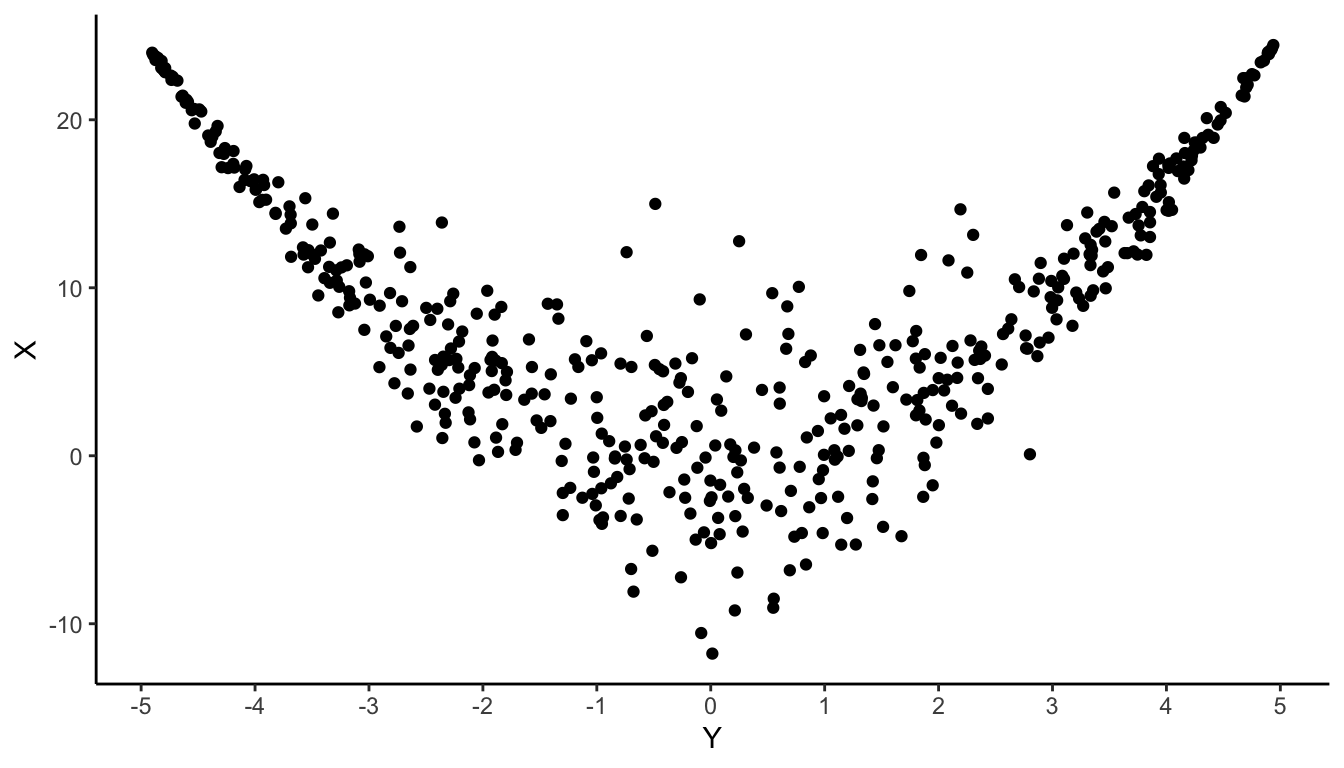
\includegraphics[width=1\linewidth]{bookdown-adv-stats_files/figure-latex/condexp1-1} 

}

\caption{Scatter plot of randomly sampled values from a bivariate distribution. We can see a U-shape relationship between the two random variables.}\label{fig:condexp1}
\end{figure}

The first thing to note is that there is clearly a dependence between \(X\) and \(Y\).
In the region of \(X>0\), values of \(Y\) increase as \(X\) increases, and we see a similar pattern in the opposite direction, i.e.~in the region of \(X<0\), values of \(Y\) increase as \(X\) decreases.
In other words, values of \(Y\) increases as \(|X|\) increases.
We say there is a \emph{non-linear} dependence of \(X\) on \(Y\) (a straight line plotted through the points will not sufficiently capture the relationship between them).

Next, suppose we colour the the points by the values of \(X\).
In the plot below, large values of \(X\) are coloured on the yellow end of the spectrum, while small values of \(X\) are coloured dark blue.
The marginal distribution of \(X\) is akin to ``flattening'' the horizontal axis until every point lies in a straight vertical line.
The vertical histogram on the right side gives a representation of how distributed the points are along this flat vertical line.
The \emph{mass} of the distribution seems to lie in the middle, perhaps somewhere in between 0 and 5.
If we calculated the sample mean of all the observed \(X\) values, this would given (an estimate) for the \emph{marginal} expectation of \(X\).
This is marked in the plot by the horizontal dashed line.

\begin{figure}

{\centering 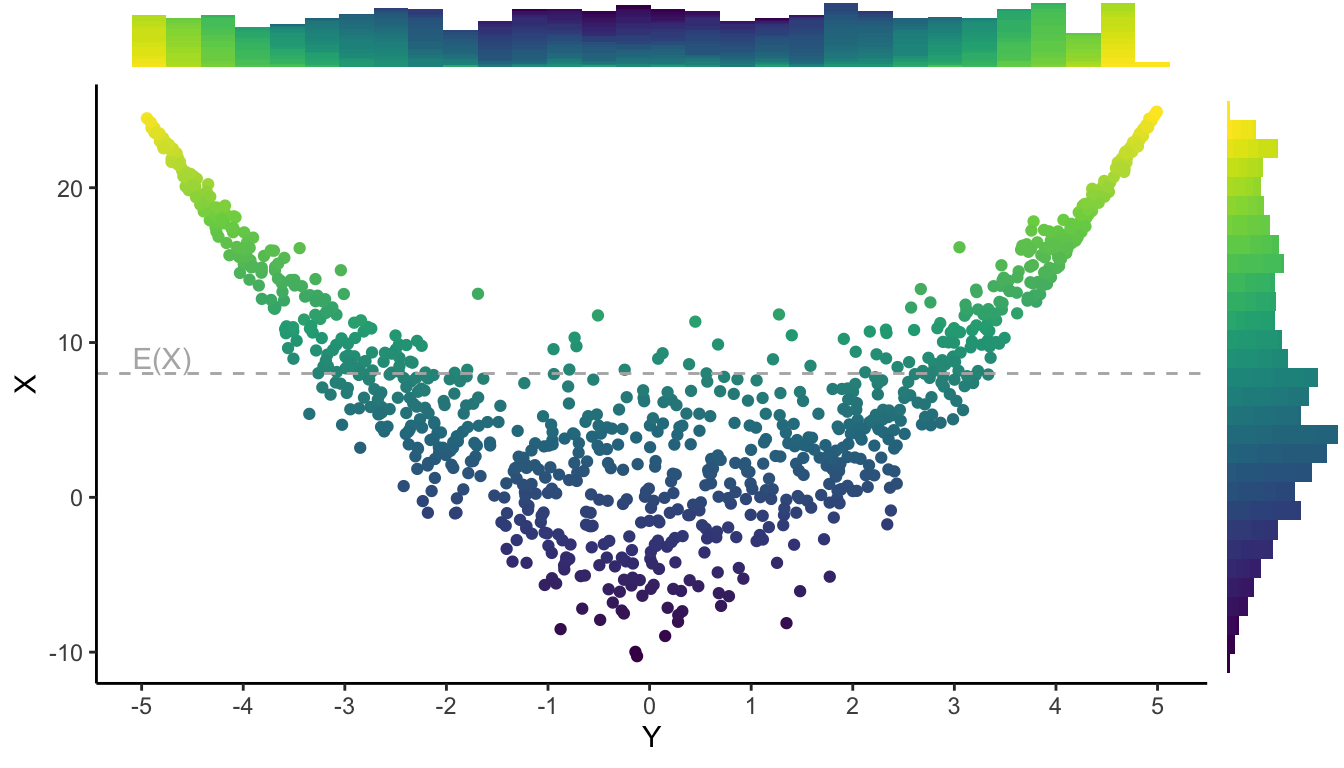
\includegraphics[width=1\linewidth]{bookdown-adv-stats_files/figure-latex/condexp2-1} 

}

\caption{Illustration of the marginal distributions of \(X\) and \(Y\) together with their respective means.}\label{fig:condexp2}
\end{figure}

Similarly, we can get the marginal distribution for \(Y\) as well as the marginal expectation of \(Y\) by flattening the vertical axis.

When we speak about ``flattening'' the horizontal axis, this is essentially what we do when we compute the marginal distribution,
\[
f_X(x) = \int_y f_{X,Y}(x,y) \dint y
\]
as we are \emph{marginalising} over the values of \(Y\).
What results is the distribution of \(X\)!

From here, we can compute the \emph{marginal} expectation of \(X\), i.e.
\[
\E(X) = \int_x x \cdot \overbrace{\left( \int_y f_{X,Y}(x,y) \dint y \right)}^{f_X(x)} \dint x
\]

Now, imagine that we concentrate on vertical strips of the scatterplot centred on various values of \(Y\).
When we concentrate on just one strip, the distribution of \(X\) then changes, and thus the expected value \emph{conditional on this value of \(Y\)} also changes.
We clearly see that the distribution changes depending on where we draw the vertical strip, i.e.~what the value of \(Y\) is.
This is the concept for \emph{conditional distributions}.

From these conditional distributions, we can clearly visualise the and \emph{conditional expectations} and \emph{conditional variances} through the boxplots at different locations of \(Y\) (see Figure \ref{fig:condexp3}).
For instance, the boxplots at \(Y=0\) are definitely wider than that at \(Y=5\)--there is more variability at \(Y=0\) and less at \(Y=5\).
Also, at \(Y=0\), the mean of the points within the green strip is about 0--we can think of this as roughly representing \(\E(X|Y=0)=0\).
The conditional mean changes for different locations of \(Y\).
For \(Y=5\) for instance, the conditional mean of \(X\) is about 20.

\begin{figure}

{\centering \includegraphics[width=1\linewidth]{bookdown-adv-stats_files/figure-latex/condexp3pdf-1} 

}

\caption{The distribution of \(X\) conditional on different values of \(Y\).}\label{fig:condexp3pdf}
\end{figure}

In Figure \ref{fig:condexp3} as well we have drawn a quadratic line through the data points.
This line actually represents the curve \(g(y)=\E(X|Y=y)\).
That is to say, the mean of \(X\) conditional on the value of \(Y=y\) is represented along this curve.
The relationship between the curve and the total expectation \(\E(X)\) is that \(\E(X)\) is the average of all values of the curve \(\E(X|Y=y)\) weighted by the probability distribution of \(Y\).
Since the distribution of \(Y\) is pretty uniform (see Figure \ref@(fig:condexp2)), this explains why the dotted horizontal line is somewhere in the middle of the black curve.
This explains the law of total expectations.

We can also illustrate the law of total variance using this graphic.
Consider any point in this scatterplot, and its distance to the overall mean \(\E(X)\).
It can be split into two parts, as follows:
\begin{equation}
\overbrace{X - \E(X)}^{\text{blue part}} = \overbrace{X - \E(X|Y)}^{\text{red part}} + \overbrace{\E(X|Y) - \E(X)}^{\text{green part}} \label{eq:condvariancebreakdown}
\end{equation}
This is illustrated in the following graphic:

\begin{figure}

{\centering 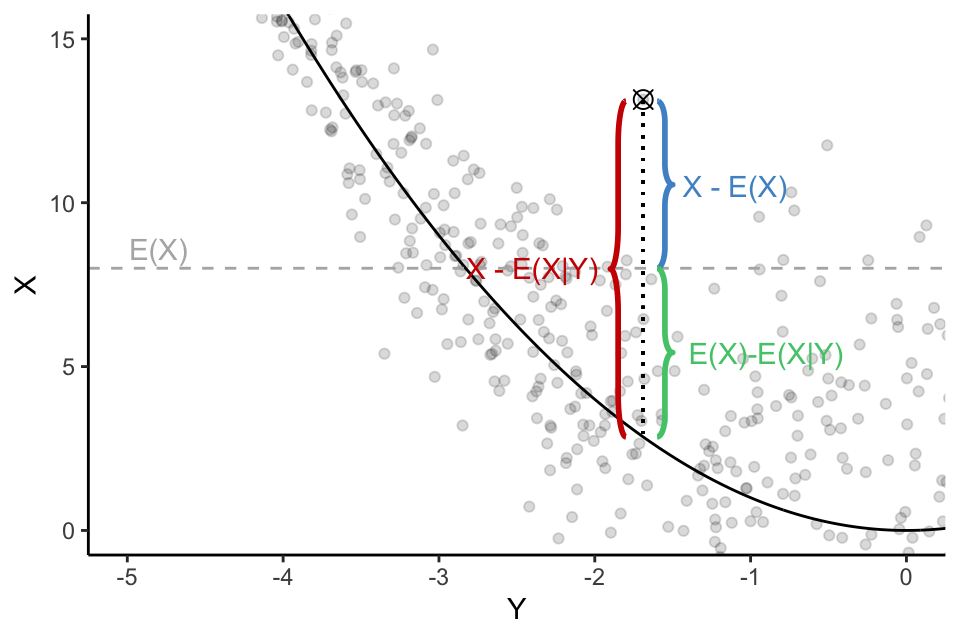
\includegraphics[width=1\linewidth]{bookdown-adv-stats_files/figure-latex/condexp4-1} 

}

\caption{The distance between any point and the grand mean is the sum of two parts: a) the distance between the point and the conditional mean; and b) the distance between the conditional mean and the grand mean.}\label{fig:condexp4}
\end{figure}

If this is the case, using the formula for the variance as well as properties of expectations on \eqref{eq:condvariancebreakdown}, we get the relationship
\begin{align*}
\{X - \E(X)\}^2 &= \left\{X - \E(X|Y) + \E(X|Y) - \E(X) \right\}^2 \\
&= \left\{X - \E(X|Y)\right\}^2 + \left\{\E(X|Y) - \E(X) \right\}^2 \\
&\hspace{2em}+ 2 \left\{X - \E(X|Y)\right\} \left\{\E(X|Y) - \E(X) \right\} \\
\Rightarrow \E\{X - \E(X)\}^2
&= E\left\{X - \E(X|Y)\right\}^2 + \E\left\{\E(X|Y) - \E(X) \right\}^2 \\
&\hspace{2em}+ \cancelto{0}{2 \E \left\{X - \E(X|Y)\right\} \left\{\E(X|Y) - \E(X) \right\}} \\
\Rightarrow \Var(X) &= \E\{\Var(X|Y) \} + \Var\{\E(X|Y)\}
\end{align*}

as required.
Some additional algebra to support the above:

\begin{align*}
\E\left\{X - \E(X|Y)\right\}^2 
&=\E\left\{\E\left[\left\{X - \E(X|Y)\right\}^2 \mid Y \right]\right\}\\
&\text{by the Law of Total Expectations} \\
&= \E\left\{\Var(X|Y) \right\}
\end{align*}

\begin{align*}
\E\left\{\E(X|Y) - \E(X) \right\}^2
&= \E\left\{\E(X|Y) - \E\big(\E(X|Y)\big) \right\}^2 \\
&- \Var\left\{ \E(X|Y) \right\}
\end{align*}

\begin{align*}
\E \bigg\{\big(X - \E(X|Y)\big) \overbrace{\big(\E(X|Y) - \E(X)\big)}^{g(Y)} \bigg\} 
&= \E\left\{g(Y) \big(X - \E(X|Y)\big) \right\}\\ 
&= \E_Y \left[ \E\left\{g(Y) \big(X - \E(X|Y)\big) \right\} \mid Y \right] \\
&= \E_Y \left[ g(Y) \left\{ \big(\E(X|Y) - \E(X|Y)\big) \right\} \mid Y \right] \\
&= 0
\end{align*}

\hypertarget{moment-generating-functions}{%
\section{Moment generating functions}\label{moment-generating-functions}}

Interestingly, the concept of \emph{moments} in statistics is borrowed from physics, in the sense that the moment of a function are measures relating to the shape of a function's graph.
Wikipedia states that if a function represents mass, the first moment is the center of the mass, and the second moment is the rotational inertia.
In statistics, we concern ourselves with moments of probability functions.

\begin{definition}[Moments]
The \(k\)th \emph{moment} of a random variable \(X\) is
\[
m_k = \E(X^k).
\]
The \(k\)th \emph{central moment} of \(X\) is
\[
\mu_k = \E\left[(X-\mu)^k \right],
\]
where \(\mu=\mu_1'=\E(X)\).
The \(k\)th \emph{standardised moment} of \(X\) is
\[
\tilde\mu_k = \E\left[\left(\frac{X-\mu}{\sigma}\right)^k \right],
\]
where \(\sigma^2 = \mu_2\).
\end{definition}

Some common moments of a random variable \(X\) are as follows.

\begin{itemize}
\tightlist
\item
  The first moment is the \emph{mean} or \emph{expectation}.
\item
  The second central moment is the \emph{variance}.
\item
  The third standardised moment is the \emph{skewness}, a measure of asymmetry of the pdf about its mean.
\item
  The fourth standardised moment is the \emph{kurtosis}, a measure of ``tailed-ness'' of aa pdf.
\end{itemize}

\hypertarget{moment-generating-functions-1}{%
\subsection{Moment generating functions}\label{moment-generating-functions-1}}

There is a function in statistics which is useful for finding moments of a random variable, called the \emph{moment generating function}.

\begin{definition}[Moment generating function]
Let \(X\sim f_X(x)\). For \(t\in\bbR\), the \emph{moment generating function (mgf)} of \(X\) is defined by
\[
M_X(t) = \E(e^{tX}) = \begin{cases}
\sum_x e^{tx} f_X(x) &\text{if $X$ discrete} \\
\int e^{tx} f_X(x) \dint x &\text{if $X$ continuous} \\
\end{cases}
\]
provided this expectation exists in ``some neighbourhood of 0''.
\end{definition}

While the primary use of the mgf is for finding moments of a random variable, it has also these other uses (read on further down for properties of mgfs):

\begin{itemize}
\tightlist
\item
  Characterising a distribution.
\item
  Finding distributions of sums of random variables.
\item
  As a tool in statistical proofs
\end{itemize}

How exactly does it ``generate'' moments? Consider finding the first derivative of \(M_X(t)\) evaluated at \(t=0\):

\begin{align}
\frac{\ddif}{\ddif t}M_X(t) \bigg|_{t=0}
&= \frac{\ddif}{\ddif t}  \E(e^{tX}) \bigg|_{t=0} \nonumber \\
&=  \E\left[  \frac{\ddif}{\ddif t}e^{tX} \right]\bigg|_{t=0} \label{eq:mgf}   \\
&= \E[Xe^{tX}] \Big|_{t=0}  \nonumber \\ 
&= \E(X). \nonumber
\end{align}

We get exactly the first moment.
These steps can be iterated to generate the \(k\)-th moment of \(X\), i.e.~by taking \(k\) derivatives and setting \(t=0\).

\begin{theorem}
If \(X\) has mgf \(M_X(t)\), then

\[
\E(X^k) = M_X^{(k)}(0) = \frac{\ddif^k}{\ddif t^k}M_X(t) \bigg|_{t=0}.
\]
That is, the \(k\)-th moment is equal to the \(k\)-th derivative of \(M_X(t)\) evaluated at \(t=0\).
\end{theorem}

There are two subtle things going on here when we use the mgf.
The first one is that obtaining moments relies on being able to \emph{interchange the order of differentiation and integration}, because for continuous distributions,
\[
\frac{\ddif}{\ddif t}  \E(e^{tX}) = \frac{\ddif}{\ddif t} \left(\int e^{tx}f_X(x)\dint x \right)
\]
and in \eqref{eq:mgf} above, it is assumed we can interchange the order of differentiation and integration so that
\[
\frac{\ddif}{\ddif t}  \E(e^{tX}) = \int \left( \frac{\ddif}{\ddif t}  e^{tx} \right) f_X(x) \dint x = \E\left(Xe^{tX}\right).
\]
For ``nice'' and well-behaved random variables, there are generally no problems.
See Section 2.4 of C\&B.

The second thing is that statement about the expectation ``existing in some neighbourhood of 0''.
This is so that when we plug in \(t=0\) in the expression for the mgf, we get a valid expectation.
If this is not the case, then the moment does not exist.

\begin{example}
Let \(X\sim\Exp(1/r)\) with \(f_X(x)=r e^{-r x}\) for \(x\in[0,\infty)\).
This is an exponential distribution with rate parameter \(r\).
Then for \(t<r\),
\begin{align*}
M_X(t) 
&= \int_0^\infty e^{tx}\cdot r e^{- r x} \dint x  \\
&= r \int_0^\infty e^{(t- r)x} \dint x \\
&= \frac{ r}{ r-  t}.
\end{align*}
Thus, \(\E(X)=M_X'(t)\big|_{t=0}=\frac{r}{(r-t)^2}\Big|_{t=0}=1/r\).
Indeed, the expectation of the exponential distribution is given as the inverse rate.
We'll meet the exponential distribution in more detail in the next chapter.
\end{example}

Here are some properties of mgfs that are worth noting.

\begin{itemize}
\tightlist
\item
  If \(Y=aX+b\), then \(M_Y(t)=e^{bt}M_X(at)\).
\item
  If \(X_1,\dots,X_n\) are independent and \(Y=\sum_{i=1}^n X_i\), then \(M_Y(t)=\prod_{i=1}^n M_{X_i}(t)\).
\item
  If \(X\) and \(Y\) are random variables s.t. \(M_X(t)=M_Y(t)\) for all \(t\) in an open interval around 0, then \(F_X(x)=F_Y(x)\) for all \(x\).
\end{itemize}

The mgf has the property that it uniquely defined a distribution.
That is, if two distributions have identical mgfs then they have the same distribution.
This way, we can usually identify distributions from a recognisable mgf.
We'll see some examples of this in action in the later chapters.

\hypertarget{exercises}{%
\section{Exercises}\label{exercises}}

\begin{enumerate}
\def\labelenumi{\arabic{enumi}.}
\item
  Using only the three axioms of probability, prove the following statements:

  \begin{enumerate}
  \def\labelenumii{(\alph{enumii})}
  \tightlist
  \item
    \(\Pr(\{\})=0\)
  \item
    If \(A \subseteq B\) then \(\Pr(A) \leq \Pr(B)\) \emph{Hint: Write \(B = A \cup (B \cap A^c)\)}
  \item
    \(0 \leq \Pr(A) \leq 1\)
  \item
    \(\Pr(A^c)=1-\Pr(A)\)
  \item
    If \(A \cap B = \{\}\), then \(\Pr(A\cup B) = \Pr(A) + \Pr(B)\)
  \end{enumerate}
\item
  This is called the ``Monty Hall Problem''. A prize is placed at random behind one of three doors. You pick a door. To be concrete, let's suppose you always pick door 1. Now Monty Hall chooses one of the other two doors, opens it and shows you that it is empty. He then gives you the opportunity to keep your door or switch to the other unopened door. Should you stay or switch? Intuition suggests it doesn't matter. The correct answer is that you should switch. Prove it.

  It will help to specify the sample space and the relevant events carefully. Thus write \(\Omega = \big\{(\omega_1,\omega_2) \,|\, \omega_i \in \{1,2,3\}\big\}\) where \(\omega_1\) is where the prize is and \(\omega_2\) is the door Monty opens.
\item
  There are three cards. The first is green on both sides, the second is red on both sides and the third is green on one side and red on the other. We choose a card at random and we see one side (also chosen at random). If the side we see is green, what is the probability that the other side is also green? Many people intuitively answer 1/2. Show that the correct answer is 2/3.
\item
  \begin{enumerate}
  \def\labelenumii{(\alph{enumii})}
  \item
    For independent events \(A_1,\dots,A_n\), show that
    \[\Pr(A_1 \cup \cdots \cup A_n) = 1 - \prod_{i=1}^n \big(1 - \Pr(A_i)\big).\]
  \item
    A pair of dice is rolled \(n\) times. How large must \(n\) be so that the probability of rolling at least one double six is more than 1/2?
  \end{enumerate}
\item
  The probability that a child has blue eyes is 1/4. Assume independence between children. Consider a family with 3 children.

  \begin{enumerate}
  \def\labelenumii{(\alph{enumii})}
  \tightlist
  \item
    If it is known that at least one child has blue eyes, what is the probability that at least two children have blue eyes?
  \item
    If it is known that the youngest child has blue eyes, what is the probability that at least two children have blue eyes?
  \end{enumerate}
\item
  Prove the following statements.

  \begin{enumerate}
  \def\labelenumii{(\alph{enumii})}
  \tightlist
  \item
    If \(A \perp B\), then \(A^c \perp B^c\).
  \item
    \(\Pr(A \cap B \cap C) = \Pr(A| B \cap C)\Pr(B|C)\Pr(C)\).
  \end{enumerate}
\item
  Let \(X\) be distributed according to
  \[
  f_X(x) = \begin{cases}
   1/4&0<x<1\\
   3/8&3<x<5 \\
   0&\text{otherwise}
  \end{cases}
  \]

  \begin{enumerate}
  \def\labelenumii{(\alph{enumii})}
  \tightlist
  \item
    Show that \(f_X\) is indeed a probability density function.
  \item
    Find the cumulative distribution function of \(X\).
  \end{enumerate}
\item
  Suppose we toss a coin once and let \(p\) be the probability of heads. Let \(X\) denote the number of heads and let \(Y\) denote the number of tails. Prove that \(X\) and \(Y\) are independent.
\item
  Let
  \[
  f_{X,Y}(x,y) = \begin{cases}
   c(x+y^2) &0\leq x \leq 1, 0\leq y \leq 1 \\
   0&\text{otherwise}
  \end{cases}
  \]

  \begin{enumerate}
  \def\labelenumii{(\alph{enumii})}
  \tightlist
  \item
    Find the value of \(c\).
  \item
    Find \(\Pr(X<1/2 | Y=1/2)\).
  \end{enumerate}
\item
  Consider a sequence of independent coin flips, each of which has probability \(p\) of being heads. Define a random variable \(X\) as the length of the run (of either heads or tails) started by the first trial. For example, \(X=3\) if either \(TTTH\) or \(HHHT\) is observed. Find the distribution of \(X\) and find \(\E(X)\).
\item
  For a random variable \(X\) with mean \(\mu\) and variance \(\Var(X)\) and any given constant \(c\in\bbR\), prove that

  \begin{enumerate}
  \def\labelenumii{(\alph{enumii})}
  \tightlist
  \item
    \(\Var(X) = \E(X^2) - \mu^2\).
  \item
    \(\Var(X) = \E\big(X(X-1)\big) +\mu -\mu^2\).
  \item
    \(\E\big((X-c)^2\big) = \Var(X) + (\mu-c)^2\) so that the minimum mean squared deviation occurs when \(c=\mu\).
  \end{enumerate}
\item
  Suppose we play a game where we start with \(c\) dollars. On each play of the game you either double or halve your money, with equal probability. What is your expected fortune after \(n\) trials?
\item
  Let \(X_1,\dots,X_n\iid \Unif(0,1)\) and let \(Y_n=\max\{X_1,\dots,X_n\}\). Find \(\E(Y_n)\). \emph{Hint: Find out the distribution of \(Y_n\) by looking at the cdf of \(Y_n\).}
\item
  Let \(X\sim\Unif(0,1)\). Let \(0<a<b<1\). Let
  \[
   Y = \begin{cases}
  1 & 0<x<b \\
  0 &\text{otherwise}
   \end{cases}
  \]
  and let
  \[
   Z = \begin{cases}
  1 & a<x<1 \\
  0 &\text{otherwise}
   \end{cases}
  \]
\end{enumerate}

\begin{enumerate}
\def\labelenumi{(\alph{enumi})}
\tightlist
\item
  Are \(Y\) and \(Z\) independent? Why/why not?\\
\item
  Find \(\E(Y|Z)\). \emph{Hint: What values \(z\) can \(Z\) take? Find first \(\E(Y|Z=z)\).}
\end{enumerate}

\hypertarget{hand-in-questions}{%
\subsection*{Hand-in questions}\label{hand-in-questions}}
\addcontentsline{toc}{subsection}{Hand-in questions}

\begin{enumerate}
\def\labelenumi{\arabic{enumi}.}
\item
  A certain river floods every year. Suppose that the low-water mark is set at 1 and the high-water mark \(Y\) has distribution function
  \[
  F_Y(y) = \Pr(Y\leq y) = 1 - \frac{1}{y^2}, \hspace{2em} 1\leq y<\infty
  \]

  \begin{enumerate}
  \def\labelenumii{(\alph{enumii})}
  \tightlist
  \item
    Verify that \(F_Y(y)\) is a cdf. \textbf{{[}1 mark{]}}
  \item
    Find \(f_Y(y)\), the pdf of \(Y\). \textbf{{[}2 marks{]}}
  \item
    If the low-water mark is reset at 0 and we use a unit of measurement that is 1/10 of that given previously, the height water mark becomes \(Z=10(Y-1)\). What is the expected value of \(Z\)? \textbf{{[}2 marks{]}}
  \end{enumerate}
\item
  A pdf is defined by
  \[
  f_{X,Y}(x,y) = \begin{cases}
   c(x+2y) &0\leq x \leq 2, 0\leq y \leq 1 \\
   0&\text{otherwise}
  \end{cases}
  \]

  \begin{enumerate}
  \def\labelenumii{(\alph{enumii})}
  \tightlist
  \item
    Find the value of \(c\). \textbf{{[}1 mark{]}}
  \item
    Find the marginal distribution of \(X\). \textbf{{[}2 marks{]}}
  \item
    Find the joint cdf of \(X\) and \(Y\). \textbf{{[}2 marks{]}}
  \end{enumerate}
\item
  Suppose we generate a random variable \(X\) in the following way. First we flip a fair coin. If the coin is heads, take \(X\) to have a \(\Unif(0,1)\) distribution. If the coin is tails, take \(X\) to have a \(\Unif(3,4)\) distribution.

  \begin{enumerate}
  \def\labelenumii{(\alph{enumii})}
  \tightlist
  \item
    Find the mean of \(X\). \textbf{{[}2 marks{]}}
  \item
    Find the standard deviation of \(X\). \textbf{{[}3 marks{]}}
  \end{enumerate}
\end{enumerate}

\hypertarget{commonly-used-probability-models}{%
\chapter{Commonly-used probability models}\label{commonly-used-probability-models}}

Distributions in statistics serve two main purposes:

\begin{enumerate}
\def\labelenumi{\arabic{enumi}.}
\tightlist
\item
  To describe the assumed behaviour of the observations made in an experiment, survey or other study;
\item
  To calibrate the values of derived statistics used in constructing confidence regions, hypothesis tests, etc.
\end{enumerate}

Some distributions are much used for both purposes (the normal distribution being the prime example).

In this chapter, we will focus on some distributions used for the first purpose.
Distributions used mainly for the second purpose (these include the \(\chi^2\), \(t\) and \(F\) distributions) will be described later, in Chapter 3.

We will meet a \emph{family} of distributions--a family which is indexed by one or more \emph{parameters} (c.f. parametric family).
This allow us to vary certain characteristics of the distribution while staying with one functional form.
For example, consider several random variables \(X_k\sim\N(k,1)\), for a couple of values of \(k\).
That is, \(X_k\) is a normal distribution with mean \(k\) and variance 1.
These are distinct distributions (e.g., \(\Pr(X_{10} < 0) \ll \Pr(X_0 < 0)\)) yet have similar characteristics (e.g.~they are all bell-shaped).

\begin{center}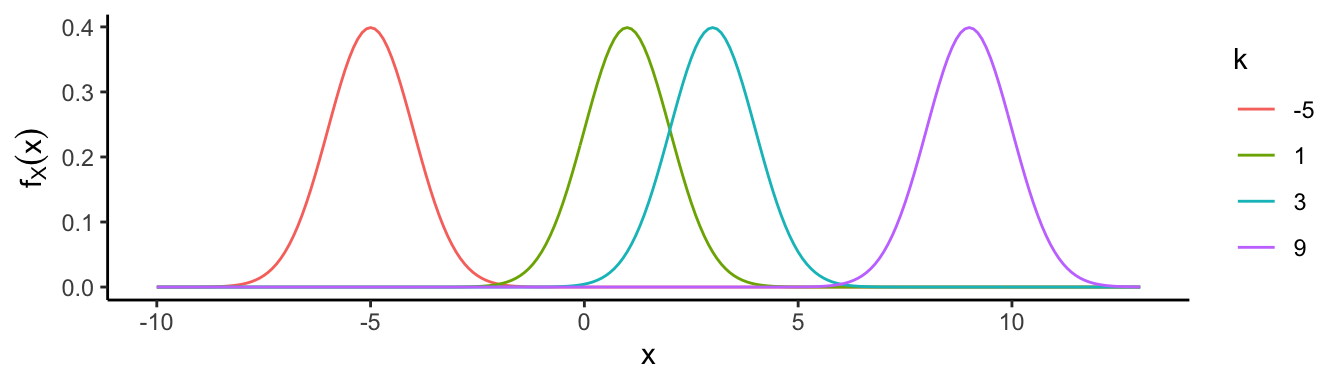
\includegraphics[width=1\linewidth]{bookdown-adv-stats_files/figure-latex/normaldist_param-1} \end{center}

Starting from this chapter onwards, we will denote probability using the notation `\(\Pr\)' rather than the blackboard bold symbol `\(\bbP\)' as we did previously.
Either symbol is fine, but I feel `\(\bbP\)' is used to denote the probability measure of an event, and is traditionally used in probability theory.
Of course when we write \(\Pr(X<a)\) we really mean the probability measure of the event \(\{ X < a\}\) so really the measure theoretic stuff is there regardless (or maybe we should write it \(\bbP(\{X < a\})\) to be proper?).

The point is, write it any way you want. It should be fine. Just so you know, I'll be using `\(\Pr\)' from here on out.

\hypertarget{learning-objectives-1}{%
\subsection*{Learning objectives}\label{learning-objectives-1}}
\addcontentsline{toc}{subsection}{Learning objectives}

By the end of this chapter, you will be:

\begin{itemize}
\tightlist
\item
  Familiar with commonly used discrete and continuous probability models, including their general properties and characteristics, and situations in which that distribution is used to model data.
\item
  Able to compute probabilities involving normal distributions using the standard normal tables.
\item
  Discovering some relationships between certain distributions, and how these relationships can be exploited in approximate calculations.
\end{itemize}

\hypertarget{readings-1}{%
\subsection*{Readings}\label{readings-1}}
\addcontentsline{toc}{subsection}{Readings}

\begin{itemize}
\tightlist
\item
  Casella and Berger (2002)

  \begin{itemize}
  \tightlist
  \item
    Chapter 3, sections 3.1 3.2 3.3
  \end{itemize}
\item
  Wasserman (2004)

  \begin{itemize}
  \tightlist
  \item
    Chapter 2, sections 2.3 and 2.4.
  \item
    Chapter 3, section 3.6.
  \end{itemize}
\item
  Topics not covered: Cauchy, lognormal and double exponential (Laplace) distributions, exponential families, location and scale families
\end{itemize}

\hypertarget{discrete-models}{%
\section{Discrete models}\label{discrete-models}}

In this section, we'll be describing commonly used \textbf{discrete} probability distributions.

\hypertarget{point-mass-distribution}{%
\subsection{Point mass distribution}\label{point-mass-distribution}}

The random variable \(X\) has a point mass distribution at \(a\), written \(X\sim \delta_a\), if \(\Pr(X=a) = 1\), in which case
\[
F(x) = \begin{cases}
0 &x<a \\
1 &x\geq a.
\end{cases}
\]

The probability mass function is \(f(x)=1\) for \(x=a\), and 0 otherwise.

\begin{figure}

{\centering 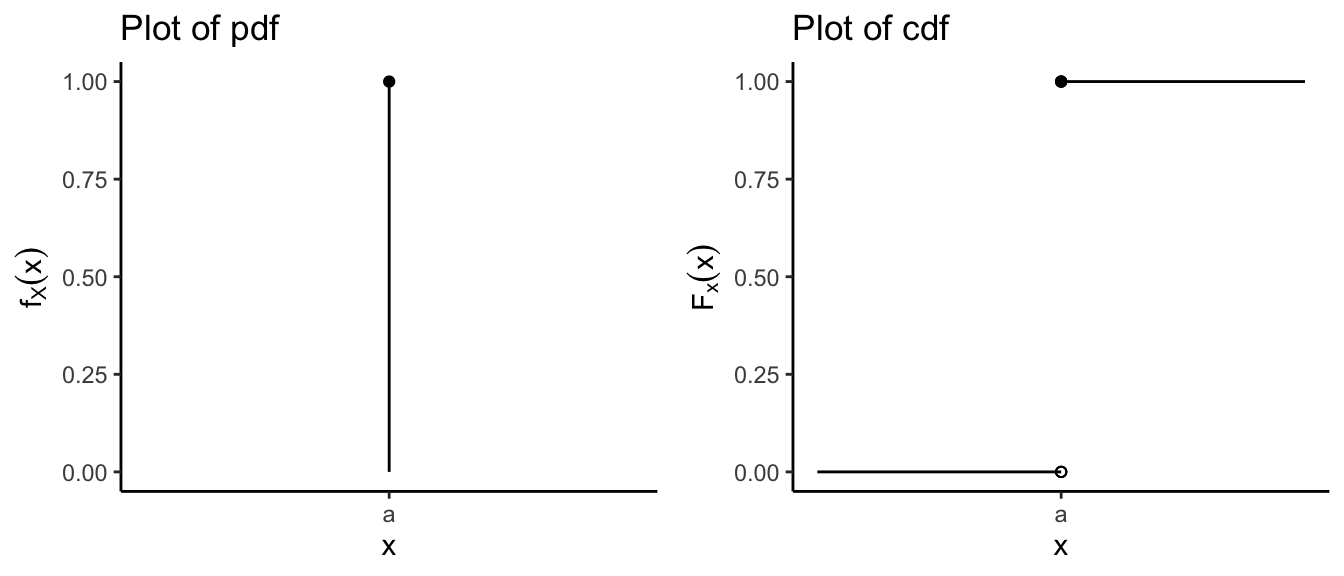
\includegraphics[width=1\linewidth]{bookdown-adv-stats_files/figure-latex/pointmasspdfcdf-1} 

}

\caption{Pdf and cdf of the point mass distribution.}\label{fig:pointmasspdfcdf}
\end{figure}

The mean and variance are trivial: \(\E(X)=a\) and \(\Var(X)=0\), because the ``random'' variable \(X\) takes on the value \(a\) with probability 1 (certainty).

There isn't much practical use for point mass distributions to be honest, but sometimes they are used to describe \emph{mixture} distributions.
For example, a random variable might be equal to \(0\) half of the time, but may be normally distributed the other half of the time.

\hypertarget{uniform-distribution}{%
\subsection{Uniform distribution}\label{uniform-distribution}}

Let \(k>1\) be a given integer. The discrete uniform distribution on \(\{1,\dots,k\}\) has pmf
\[
f(x) = \frac{1}{k}, \hspace{2em} x=1,\dots,k.
\]
We write \(X\sim\Unif\{1,\dots,k\}\). Its mean and variance are

\begin{itemize}
\tightlist
\item
  \(\E(X)=\frac{k+1}{2}\); and
\item
  \(\Var(X)=\frac{k^2-1}{12}\).
\end{itemize}

The mean of the discrete uniform is intuitive; it is the half-way point between 1 and \(k\).
The discrete uniform (and the point mass) is appeallingly simple but has relatively few ``real'' statistical applications.

\begin{proof}
Using the arithmetic series formulae \(\sum_{i=1}^n x = n(n+1)/2\) and \(\sum_{i=1}^n x^2 = n(n+1)(2n+1)/6\), we have

\begin{align*}
\E(X) &= \sum_{x=1}^k \frac{x}{k}\\
&= \frac{k(k+1)}{2k}  \\
&= \frac{k+1}{2},
\end{align*}
and
\begin{align*}
\E(X^2) &= \sum_{x=1}^k  \frac{x^2}{k}\\
&= \frac{k(k+1)(2k+1)}{6k}  \\
&= \frac{(k+1)(2k+1)}{6},
\end{align*}
hence
\begin{align*}
\Var(X) &= \E(X^2) - \E^2(X) \\
&= \frac{(k+1)(2k+1)}{6} - \frac{(k+1)^2}{4} \\
&= \frac{2(k+1)(2k+1)-3(k+1)^2}{12} \\
&= \frac{k^2-1}{12}.
\end{align*}
\end{proof}

If \(k=1\), then it is the point mass distribution. But actually, we can use whatever labels we want for the values \(1,2,\dots,k\). For example, suppose we are picking between 3 colours uniformly, then we can describe a uniform distribution on \(\{1 = \text{red}, 2= \text{green}, 3=\text{blue} \}\).

\begin{figure}

{\centering 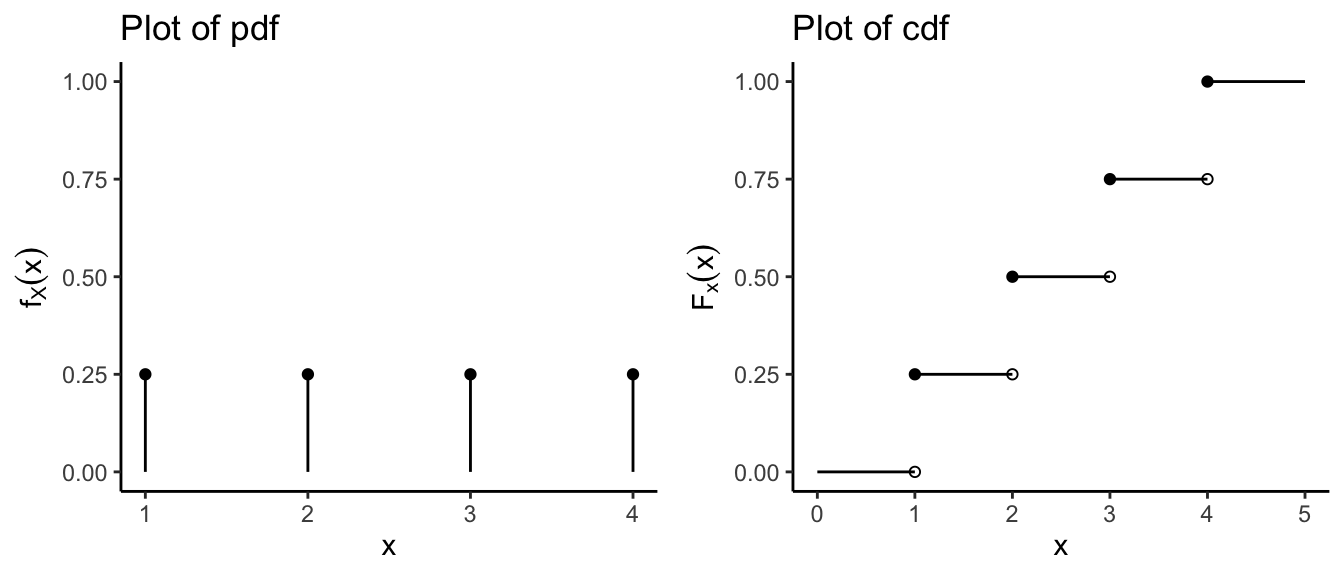
\includegraphics[width=1\linewidth]{bookdown-adv-stats_files/figure-latex/uniformpdfcdf-1} 

}

\caption{Pdf and cdf of the discrete uniform distribution for \(k=4\).}\label{fig:uniformpdfcdf}
\end{figure}

\hypertarget{bernoulli-distribution}{%
\subsection{Bernoulli distribution}\label{bernoulli-distribution}}

Suppose we are interested in the outcome of a (single) random trial, which can either be {``success''} or {``failure''} only. Examples include

\begin{itemize}
\tightlist
\item
  A coin flip can land either {Heads} or {Tails}.
\item
  The colour of the suit of a randomly drawn card from a pack of playing cards can be either {Red} or {Black}
\item
  A dice roll outcome can either be an {Even} or an {Odd} number.
\item
  Babies being born being {Girl} or {Boy}.
\end{itemize}

Typically we assign the value `1' to denote success, and `0' to denote failure.
This has no qualitative meaning whatsoever, the important thing is that there are only two distinct possible outcomes.
As a consequence, any discrete random variable that can take on only two possible outcomes is a Bernoulli random variable.

Let \(X\) be the r.v. denoting the outcome of success (\(X=1\)) or failure (\(X=0\)) of a binary trial.
Further let the pmf for \(X\) be
\[
f(x|p) = \begin{cases}
p & x=1\text{ (success)}\\
1-p &x=0 \text{ (failure)}
\end{cases}
\]
We say that \(X\) has a Bernoulli distribution written \(X\sim\Bern(p)\).

\begin{itemize}
\tightlist
\item
  The expectation is
  \[
  \E(X) = \sum_x xf(x) = 1\cdot p + 0 \cdot (1-p) = p.
  \]
\item
  The variance is
  \[
  \Var(X) = \sum_x (x-\mu)^2f(x) = (1-p)^2\cdot p + (0-p)^2 \cdot (1-p) = p(1-p).
  \]
\end{itemize}

Again the expectation is intuitive here.
If a proportion \(p\) of the time we get success, then surely the expectation must be this proportion \(p\).

The pmf for the Bernoulli distribution can also be written \(f(x)=p^x(1-p)^{1-x}\).
Try plugging in \(x=1\) and \(x=0\) into this function.
Do you get the appropriate probabilities?

\begin{figure}

{\centering 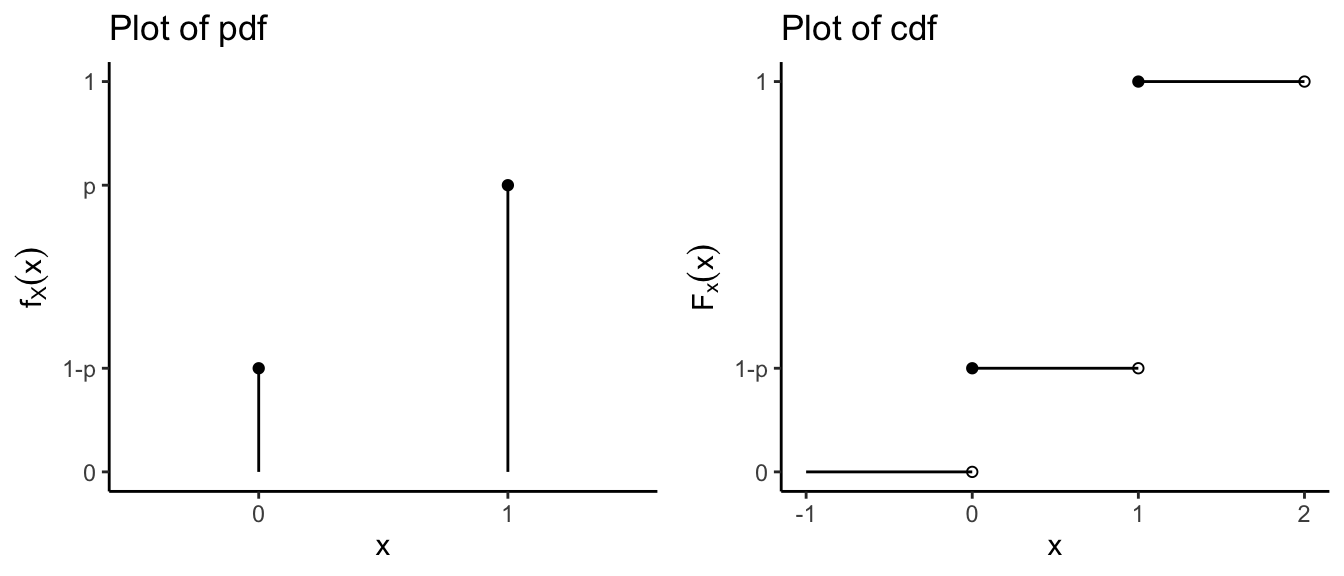
\includegraphics[width=1\linewidth]{bookdown-adv-stats_files/figure-latex/bernoullipdfcdf-1} 

}

\caption{Pdf and cdf of the Bernoulli distribution.}\label{fig:bernoullipdfcdf}
\end{figure}

\hypertarget{binomial-distribution}{%
\subsection{Binomial distribution}\label{binomial-distribution}}

A related distribution to the Bernoulli is the binomial distribution.
It describes the distribution of the number of ``successes'' in \(n\) independent and identical binary ``trials''.
That is, suppose we have a situation such that

\begin{itemize}
\tightlist
\item
  A finite number \(n\) trials are carried out.
\item
  Each trial is independent of each other.
\item
  The outcome of each trial is either success or failure (binary trials).
\item
  The probability \(0 \leq p\leq 1\) of a successful outcome is the same for each trial.
\end{itemize}

Let \(X\) be the number of success outcomes in \(n\) trials. Then \(X\) has a binomial distribution, written \(X\sim\Bin(n,p)\).
The pmf of \(X\) is
\[
f(x|n,p) = {n \choose x}p^x (1-p)^{n-x}.
\]
\(X\) has support (possible values it can take) over \(\{0,1,2,\dots,n\}\).
The mean and variance are \(\E(X)=np\) and \(\Var(X)=np(1-p)\).

\begin{proof}
Here's the proof for the mean.
\begin{align*}
\E(X) 
&= \sum_{x=0}^n x \frac{n!}{x!(n-x)!} p^x (1-p)^{n-x} \\
&= \sum_{x=1}^n x \frac{n!}{x!(n-x)!} p^x (1-p)^{n-x} \\
&=\sum_{x=1}^n n \cdot \overbrace{\frac{(n-1)!}{(x-1)!(n-x)!}}^{{n-1 \choose x-1}} \cdot p^{x-1+1} (1-p)^{(n-1)-(x-1)} \\
&= np \overbrace{\sum_{x-1=0}^n  {n-1 \choose x-1} p^{x-1} (1-p)^{n-x}}^{=1} \\
&= np. 
\end{align*}
Obtaining the variance follows similar steps.
\end{proof}

Try to replicate the proof above and obtain \(\E(X^2)\) for the binomial distribution. After that, you may obtain \(\Var(X)\) using the usual formula.
An alternative way is to use mgfs--keep on reading.

For the more astute of you, you might have realised that the binomial distribution is simply counting the number of successes in many independent Bernoulli trials.
Indeed, that is the case.

\begin{lemma}
Let \(X_1,\dots,X_n\iid\Bern(p)\), then
\[
X = \sum_{i=1}^n X_i \sim \Bin(n,p)
\]
\end{lemma}

The lemma is proven using mgfs, and is left to you as an exercise.
First, obtain the mgf for Bernoulli and binomial distributions.
Then use the sum property of the mgfs characterise the distribution of the sum.

Using the lemma above, we can more easily derive that
\[
\E(X) = \E\left(\sum_{i=1}^n X_i \right) = \sum_{i=1}^n \E(X_i) = np
\]
and
\[
\Var(X) = \Var\left(\sum_{i=1}^n X_i \right) = \sum_{i=1}^n \Var(X_i) = np(1-p)
\]
simply using properties of expectations and variances.

\begin{figure}

{\centering 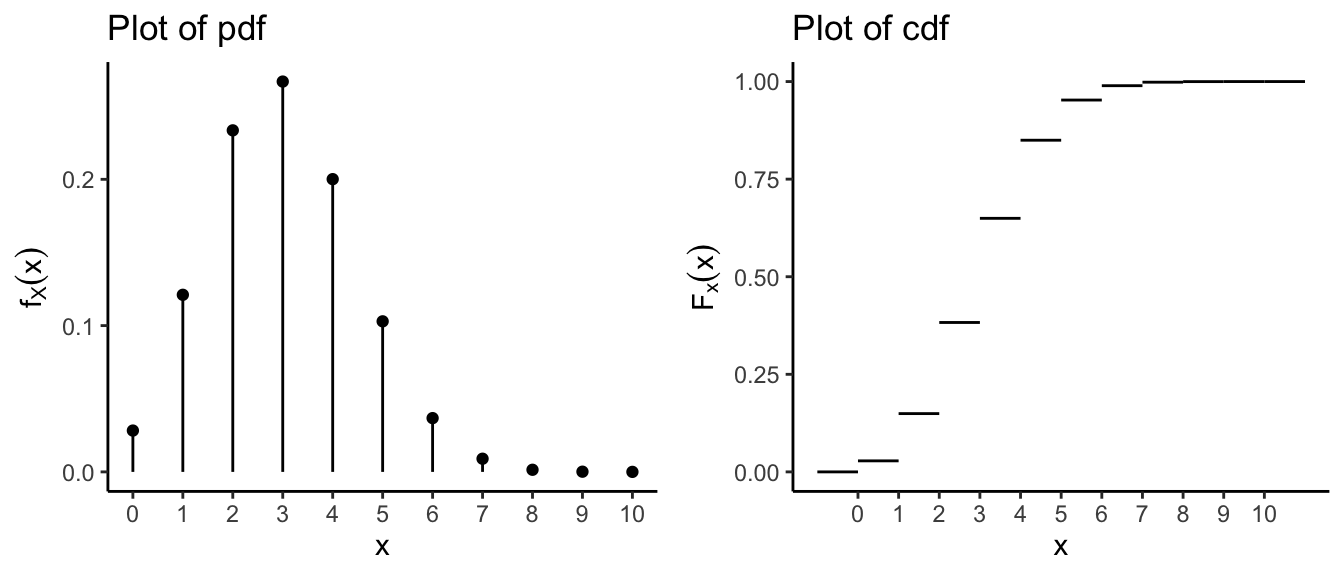
\includegraphics[width=1\linewidth]{bookdown-adv-stats_files/figure-latex/binomialpdfcdf-1} 

}

\caption{Pdf and cdf of the binomial distribution with \(p=0.3\).}\label{fig:binomialpdfcdf}
\end{figure}

\hypertarget{geometric-distribution}{%
\subsection{Geometric distribution}\label{geometric-distribution}}

The geometric distribution is a type of ``waiting time'' distribution.
It involves counting the number of Bernoulli trials to get the first success.
Let \(X\) be distributed geometrically, \(X\sim\Geom(p)\), where \(p\) is the probability of success. Clearly,
\[
  f(x|p)=(1-p)^{x-1}p.
\]
The support of \(X\) is \(\{1,2,3,\dots\}\); it is countably infinite.

This is a valid pmf since
\begin{align*}
\sum_{x=1}^\infty f(x|p) 
&= \sum_{x=1}^\infty (1-p)^{x-1}p  \\
&= \frac{p}{1-(1-p)} = 1.
\end{align*}

This required knowledge of the infinite geometric series \(\sum_{k=0}^\infty ar^k = a/(1-r)\) for \(|r|<1\).
The mean and variance of the geometric distribution are:

\begin{itemize}
\tightlist
\item
  \(\E(X)=\frac{1}{p}\). The smaller the \(p\), the longer we have to wait for a success.
\item
  \(\Var(X)=\frac{1-p}{p^2}\).
\end{itemize}

There is another formulation for the geometric distribution: Let \(Y\) be the number of failures before the first success occurs. Then
\[
f(y|p) = (1-p)^yp.
\]
\(Y\) has support \(\{0,1,2,\dots\}\). \(X\) and \(Y\) are related through \(Y=X-1\). Thus it is easy to check
that
\[
\E(Y) = \frac{1-p}{p} \text{ and } \Var(Y)=\frac{1-p}{p^2}.
\]
We shall mainly use the first version of the geometric distribution in this course, but be aware of the alternative version as well.

\begin{figure}

{\centering 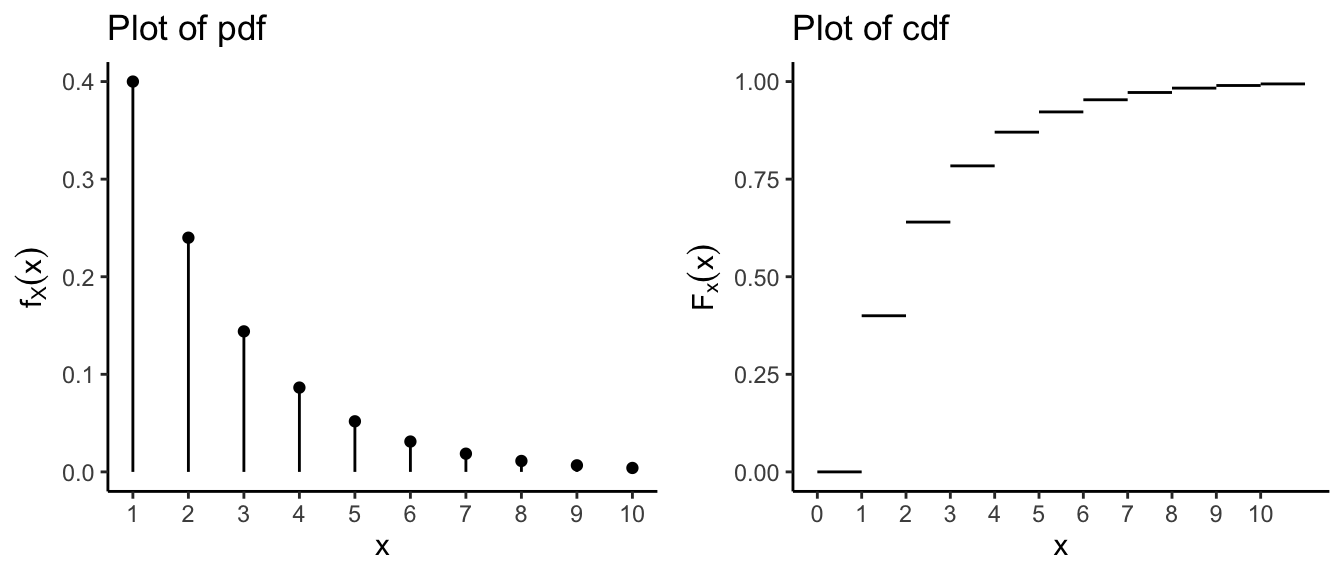
\includegraphics[width=1\linewidth]{bookdown-adv-stats_files/figure-latex/geometricpdfcdf-1} 

}

\caption{Pdf and cdf of the geometric distribution with \(p=0.4\).}\label{fig:geometricpdfcdf}
\end{figure}

\hypertarget{negative-binomial}{%
\subsection{Negative binomial}\label{negative-binomial}}

Suppose we count the number of Bernoulli trials required to get a fixed number of successes, \(r\), each with probability of success \(p\).
This leads to the negative binomial distribution.
Denote this by \(X\sim\NBin(r,p)\). The pmf is
\[
  f(x|r,p)= {x-1 \choose r-1} p^r (1-p)^{x-r}.
\]

The pmf is easy to justify: In order to get \(X=x\), a total of \(r-1\) successes must have occurred in the previous \(x-1\) number of trials. Then, the pmf follows directly from the binomial pmf.

Clearly, the support of \(X\) is \(\{r, r+1, r+2, \dots \}\).
The expectation and variance of \(X\) are

\begin{itemize}
\tightlist
\item
  \(\E(X)=\frac{r}{p}\).
\item
  \(\Var(X)=\frac{r(1-p)}{p^2}\).
\end{itemize}

Note that if \(r=1\), then \(X\) is the geometric distribution.

The name `negative binomial' comes from noting that \(Y=X-r\), the number of failures seen before the \(r\)th success, has pmf
\[
  f(y|r,p) = (-1)^y{-r \choose y} p^r(1-p)^{r-y},
\]
which looks suspiciously close to the binomial pmf\footnote{Details in C\&B, p.95}.

\begin{figure}

{\centering 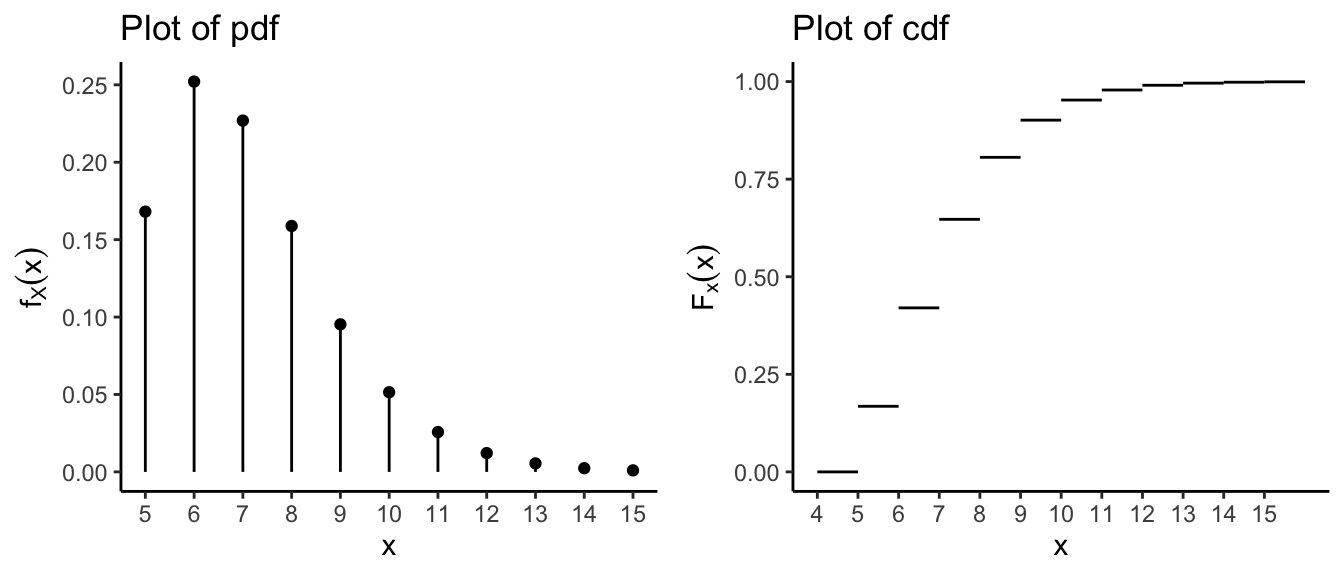
\includegraphics[width=1\linewidth]{bookdown-adv-stats_files/figure-latex/negbinomialpdfcdf-1} 

}

\caption{Pdf and cdf of the negative binomial distribution with \(p=0.3\) and \(r=5\).}\label{fig:negbinomialpdfcdf}
\end{figure}

Just a caution to say that the negative binomial has many different parameterisations.
It all depends whether

\begin{itemize}
\tightlist
\item
  The random variable \(X\) is counting the number of trials until a fixed success, or counting the number of successes before a fixed number of failures occur;
\item
  \(p\) denotes success or failure;
\item
  \(r\) denotes success or failure.
\end{itemize}

See here for more details: \url{https://en.wikipedia.org/wiki/Negative_binomial_distribution\#Alternative_formulations}

\hypertarget{poisson-distribution}{%
\subsection{Poisson distribution}\label{poisson-distribution}}

The Poisson is the most standard assumption for the distribution of a count of events that occur (separately and independently, by assumption) in time or space. Some examples:

\begin{itemize}
\tightlist
\item
  Amount of e-mails received in 24-hour period.
\item
  Number of calls received by a call centre per hour.
\item
  The number of photons hitting a detector in a particular time interval.
\item
  The number of patients arriving in an emergency room between 10pm and 11pm.
\end{itemize}

Let \(X\) be the number of occurrences in this interval, such that the mean number of occurrences \(\lambda\) in the given interval (sometimes called the rate or intensity) is known and is finite. Then \(X\sim\Pois(\lambda),\) and
\[
f(x|\lambda) = \frac{e^{-\lambda}\lambda^x}{x!},
\]
for \(x=0,1,2,\dots\)

To work out the mean, we make use of the Taylor series expansion.
Recall that \(e^x=\sum_{k=0}^\infty \frac{x^k}{k!}\).
Using this fact we can derive the moments through the mgf.

\begin{align*}
M_X(t)
&= \sum_{x=0}^\infty \frac{e^{tx} e^{-\lambda}\lambda^x}{x!} \\
&= e^{-\lambda} \sum_{x=0}^\infty \frac{(\lambda e^t)^x}{x!} \\
&= e^{-\lambda}e^{\lambda e^t} = \exp\{\lambda(e^t - 1) \}.
\end{align*}

Hence \(\E(X)=M_X'(0)=\lambda\) and \(\E(X^2)=M_X''(0)=\lambda^2+\lambda\), so \(\Var(X)=\E(X^2)-\E(X)=\lambda\).

The Poisson family is closed under addition.
If \(X\) and \(Y\) are independent Poisson r.v. with means \(\lambda\) and \(\mu\), then
\[
X+Y \sim \Pois(\lambda + \mu)
\]

The proof uses mgf and the characterizing property of the mgf.

Have a go at the proof using properties of the mgf.

\begin{figure}

{\centering 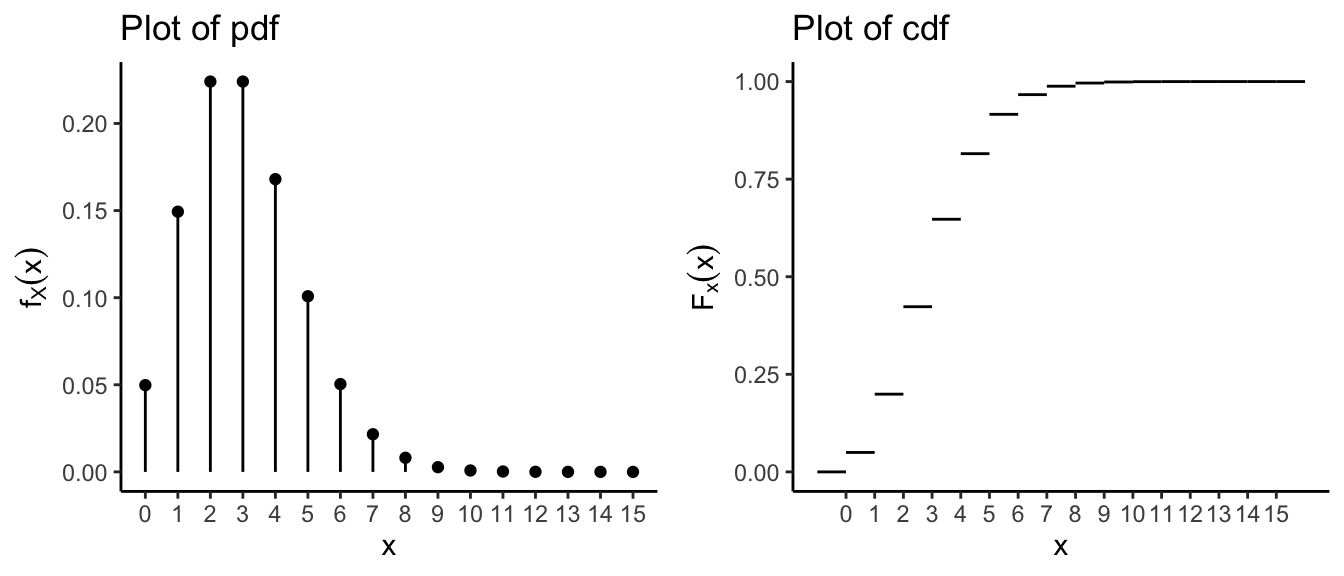
\includegraphics[width=1\linewidth]{bookdown-adv-stats_files/figure-latex/poissonpdfcdf-1} 

}

\caption{Pdf and cdf of the negative binomial distribution with \(\lambda=3\).}\label{fig:poissonpdfcdf}
\end{figure}

\hypertarget{continuous-models}{%
\section{Continuous models}\label{continuous-models}}

In this section, we'll study commonly used continuous distributions.

\hypertarget{continuous-uniform-distribution}{%
\subsection{Continuous uniform distribution}\label{continuous-uniform-distribution}}

The continuous uniform distribution is usually taken to have support on an interval, say \(a \leq x \leq b\). Let \(X\sim\Unif(a,b)\). The pdf is
\[
  f_X(x) = \frac{1}{b-a}
\]
for \(x\in[a,b]\) and 0 otherwise.
The mean and variance are

\begin{itemize}
\tightlist
\item
  \(\E(X)=\frac{a+b}{2}\).
\item
  \(\Var(X)=\frac{(a-b)^2}{12}\).
\end{itemize}

Note the similarities between the means and variances above and in the discrete case!

The plot of the pdf gives a ``rectangular'' shape, so probabilities can also be found geometrically, as we previously saw in \protect\hyperlink{exm:unitsquare}{Chapter 1}.

\begin{figure}

{\centering 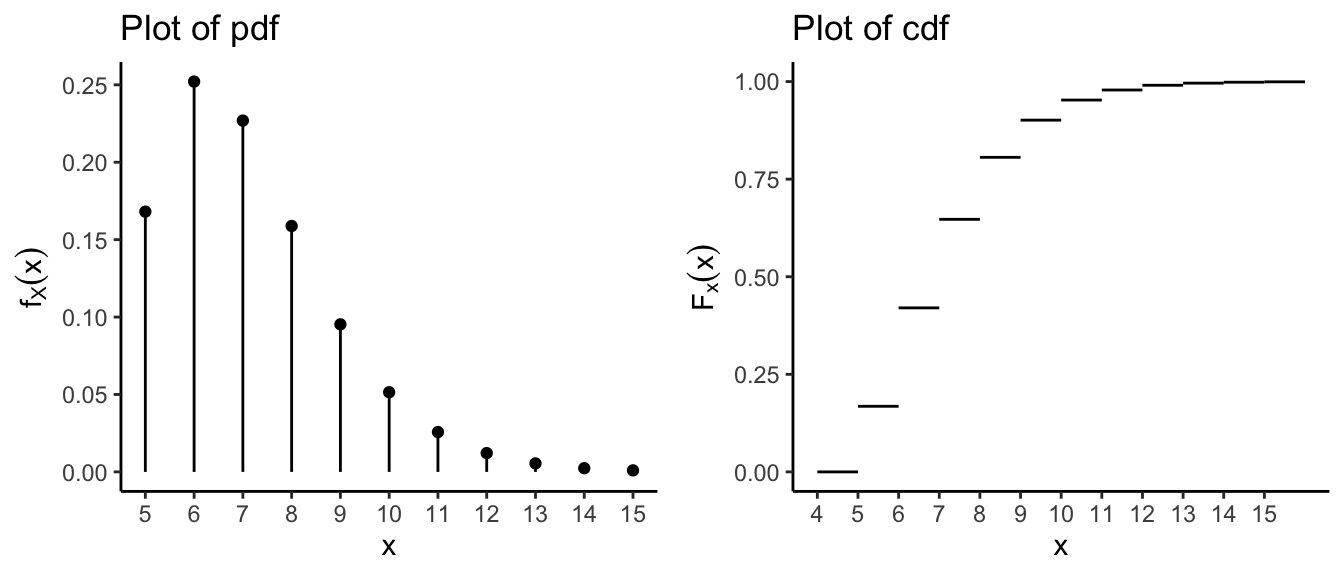
\includegraphics[width=1\linewidth]{bookdown-adv-stats_files/figure-latex/uniformctspdfcdf-1} 

}

\caption{Pdf and cdf of the negative binomial distribution with \(p=0.3\) and \(r=5\).}\label{fig:uniformctspdfcdf}
\end{figure}

\hypertarget{exponential-distribution}{%
\subsection{Exponential distribution}\label{exponential-distribution}}

The exponential distribution is often used to describe the distribution of measured time intervals `duration data' or `waiting-time data'. E.g.

\begin{itemize}
\tightlist
\item
  the amount of time until an earthquake occurs.
\item
  the time between two lightbulbs failing.
\item
  the length (in minutes) of faculty staff meetings at UBD.
\item
  the average waiting time at a hospital's A\&E.
\end{itemize}

Let \(X\sim\Exp(\lambda)\).
The pdf is
\[
f_X(x) = \frac{1}{\lambda} e^{-x/\lambda}.
\]

\(X\) has support over \([0,\infty)\), and \(\lambda >0\) is known as the ``scale'' parameter. The value \(r=1/\lambda\) is known as the ``rate''. The mean and variance are:

\begin{itemize}
\tightlist
\item
  \(\E(X)=\lambda\).
\item
  \(\Var(X)=\lambda^2\).
\end{itemize}

Since \(\lambda\) is a scale parameter, the following property holds: \(aX\sim\Exp(a\lambda)\) for \(a>0\).
What this is saying is that if we stretch (or contract) the scale of \(X\) by some amount \(a>0\), then the underlying distribution will still be the same.

The pdf experiences ``exponential decay''--long wait times between two events occurring becomes more and more unlikely.

\begin{figure}

{\centering 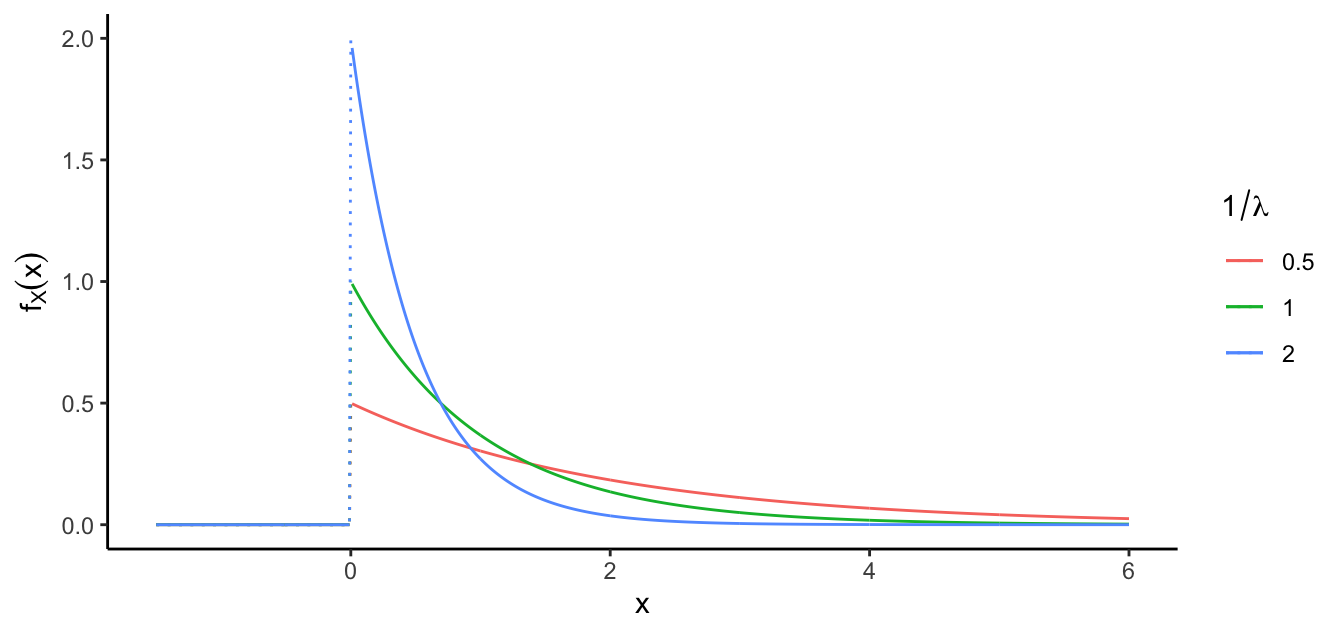
\includegraphics[width=1\linewidth]{bookdown-adv-stats_files/figure-latex/expdist-1} 

}

\caption{Pdf of the exponential distribution.}\label{fig:expdist}
\end{figure}

The exponential distribution has a very special property: it is
memoryless, in the sense that for all \(t>s>0\),
\[
\Pr(X > t+s|X>s) = \Pr(X > t)
\]

\begin{quote}
Given that we have been waiting for an event to occur for \(s\) units of time, the probability that we wait a further \(t\) units of time is independent to the first fact!
\end{quote}

For example\footnote{\footnotetext\url{https://perplex.city/memorylessness-at-the-bus-stop-f2c97c59e420?gi=3602158da66b}}, assume that bus waiting times are exponentially distributed. A memoryless wait for a bus would mean that the probability that a bus arrived in the next minute is the same whether you just got to the station or if you've been sitting there for twenty minutes already.

We can show that \(X\) is a positive r.v. and memoryless if and only if it is exponentially distributed.

You will prove the memoryless fact in one of the exercises for this chapter.

\hypertarget{gamma-distribution}{%
\subsection{Gamma distribution}\label{gamma-distribution}}

The gamma distribution generalises the exponential distribution.
It is also used for modelling durations (lengths of time intervals).
Let \(X\sim\Gamma(\alpha,\beta)\).
The pdf is
\[
  f_X(x) = \frac{1}{\Gamma(\alpha)\beta^\alpha} x^{\alpha-1} e^{- x/\beta}
\]
where \(\Gamma(\alpha)=\int_0^\infty y^{\alpha-1}e^{-y}\dint y\) is called the Gamma function.
Again here, \(X\) has support over \([0,\infty]\).
\(\alpha>0\) is the ``shape'' parameter, and \(\beta >0\) is the ``scale'' parameter.
The mean and variance are as follows:

\begin{itemize}
\tightlist
\item
  \(\E(X)=\alpha\beta\).
\item
  \(\Var(X)=\alpha\beta^2\).
\end{itemize}

Some other properties of the gamma distribution are:

\begin{itemize}
\tightlist
\item
  \(\Gamma(1,\lambda) \equiv \Exp(\lambda)\).
\item
  \(aX\sim\Gamma(\alpha,a\beta)\) for \(a>0\).
\item
  If \(X_i\sim\Gamma(\alpha_i,\beta)\), then \(\sum_{i=1}^n X_i \sim \Gamma(\sum_{i=1}^n \alpha_i,\beta)\).
\end{itemize}

Be aware that there is an alternative parameterisation of the exponential and gamma distribution using ``scale'' parameters:

\begin{itemize}
\tightlist
\item
  \(Y \sim \Exp(\lambda)\), where \(f_Y(y)=\frac{1}{\lambda}e^{-y/\lambda}\). Here \(\lambda\) is the \ldots{}
\item
  \(Y \sim \Gamma(\alpha,s)\), where \(f_Y(y)=\frac{1}{\Gamma(\alpha)s^\alpha} y^{\alpha-1} e^{-y/s}\). Here \(s\) is the \textbf{scale} parameter. The shape parameter is obtained via \(\beta=1/s\).
\end{itemize}

\begin{figure}

{\centering 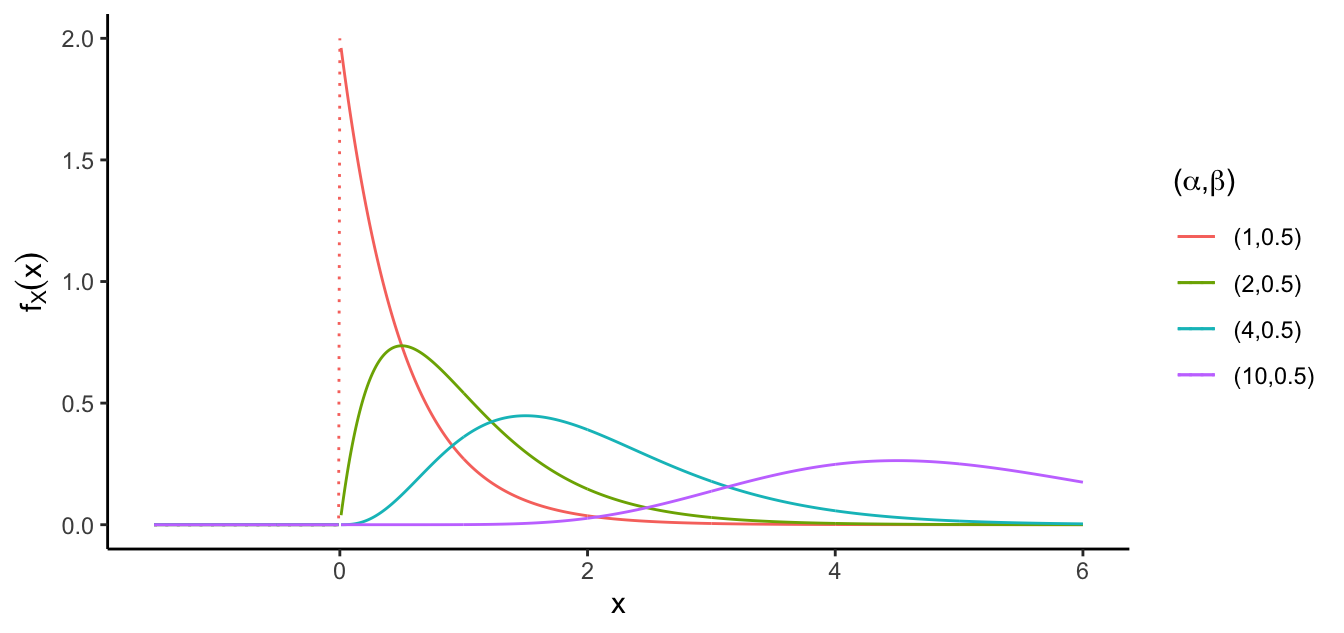
\includegraphics[width=1\linewidth]{bookdown-adv-stats_files/figure-latex/gammadist1-1} 

}

\caption{Pdf of the gamma distribution.}\label{fig:gammadist1}
\end{figure}

\hypertarget{beta-distribution}{%
\subsection{Beta distribution}\label{beta-distribution}}

The beta distributions are distributions on the unit interval \([0,1]\), or on any other interval \([a,b]\) by transformation \(X \mapsto X(b-a) + a\).
It is used to model the behaviour of random variables limited to intervals of finite length in a wide variety of disciplines.
Let \(X\sim \Betadist(\alpha,\beta)\).
The pdf is
\[
  f_X(x) = \frac{1}{B(\alpha,\beta)} x^{\alpha-1} (1-x)^{\beta-1}.
\]
where \(B(\alpha,\beta)\) is the so-called beta function
\[B(\alpha,\beta) = \frac{\Gamma(\alpha)\Gamma(\beta)}{\Gamma(\alpha+\beta)}.\]
The parameters \(\alpha>0\) and \(\beta>0\) are known as the ``shape'' parameters.
The mean and variance are

\begin{itemize}
\tightlist
\item
  \(\E(X)=\frac{\alpha}{\alpha+\beta}\).
\item
  \(\Var(X)=\frac{\alpha\beta}{(\alpha+\beta)^2(\alpha+\beta+1)}\).
\end{itemize}

On interesting fact is that when \(\alpha=\beta=1\), we have the uniform distribution.
I.e., \(\Betadist(1,1)\equiv \Unif(0,1)\).

\begin{figure}

{\centering 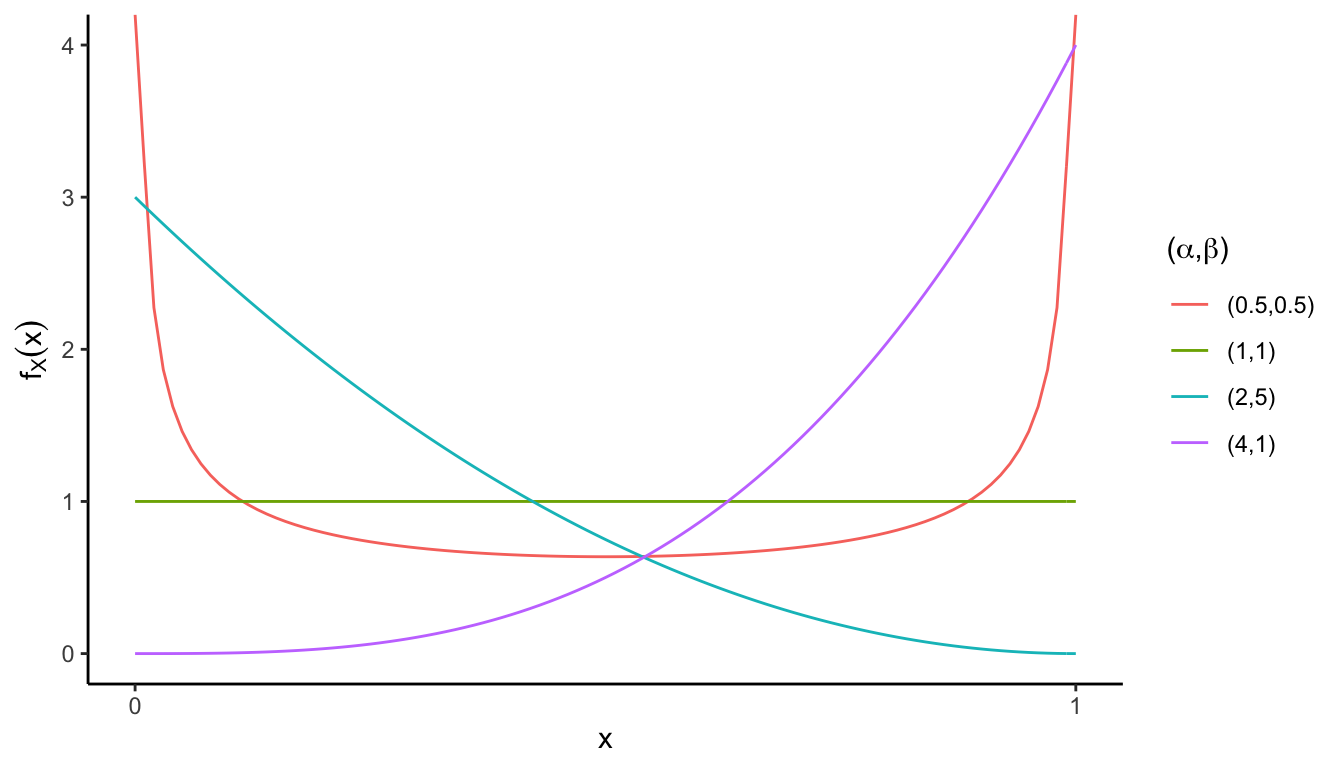
\includegraphics[width=1\linewidth]{bookdown-adv-stats_files/figure-latex/betadist-1} 

}

\caption{Pdf of the beta distribution.}\label{fig:betadist}
\end{figure}

\hypertarget{normal-distribution}{%
\section{Normal distribution}\label{normal-distribution}}

The normal distribution\footnote{Here's a nice short exploration of the normal distribution: \url{https://bookdown.org/cquirk/LetsExploreStatistics/lets-explore-the-normal-distribution.html}} is arguably the most important distribution in statistics.
There are several reasons for this, including:

\begin{itemize}
\tightlist
\item
  Many naturally occurring phenomena can be modelled as following a normal distribution.
\item
  The central limit theorem (CLT): The distribution of the mean of a sample tends to converge to a normal distribution, as more and more samples are collected.
\item
  Often, the normal distribution is used for the error term in standard statistical models (e.g.~linear regression).
\end{itemize}

Let us introduce the normal distribution.
Let \(X\) be distributed according to a normal distribution with mean \(\mu\) and variance \(\sigma^2\).
We write \(X\sim\N(\mu,\sigma^2)\).
The pdf of \(X\) is
\[
f_X(x|\mu,\sigma^2)= \frac{1}{\sigma\sqrt{2\pi}}\exp\left[-\frac{(x-\mu)^2}{2\sigma^2} \right]
\]
\(X\) has support over \(\bbR\).

The normal distribution is so important that all my previous teachers have made their students (including me) memorise the pdf of the normal distribution.
In continuing tradition, you should too!

The normal distribution is \textbf{symmetric} about \(\mu\).
The mode and median of \(X\) is also \(\mu\).

\begin{center}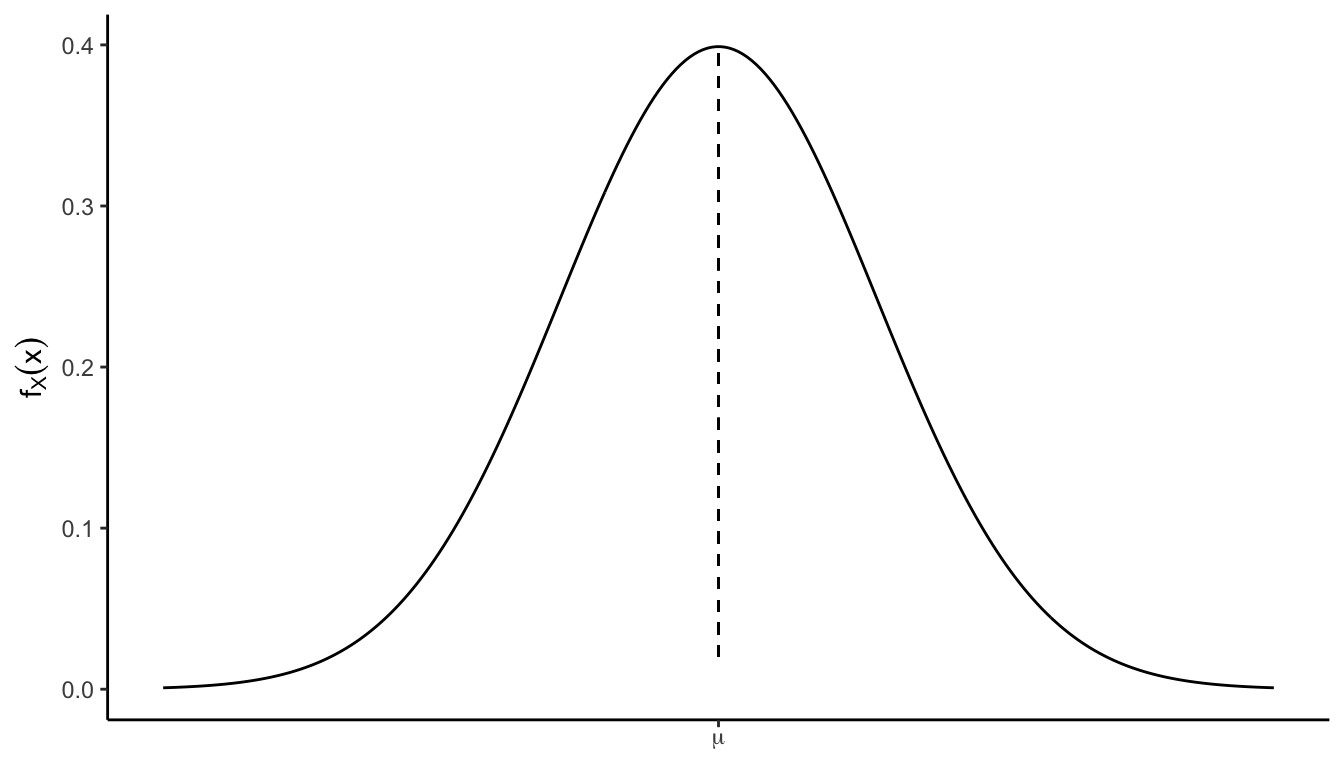
\includegraphics[width=1\linewidth]{bookdown-adv-stats_files/figure-latex/normalpdf-1} \end{center}

The celebrated mathematician Carl Friedrich Gauss has the honour of having the normal distribution named after him.
The normal distribution is often known as the Gaussian distribution.
Actually, it is named as such because the \emph{kernel} (i.e.~the insides) of the pdf contains a Gaussian function, i.e.~functions of the form \(f(x)=a\exp\left(- \frac{(x-b)^2}{2c^2} \right)\), which Gauss studied quite a lot.

\begin{figure}

{\centering \includegraphics[width=0.6\linewidth]{figure/gauss} 

}

\caption{Carl Friedrich Gauß. 30 April 1777 -- 23 February 1855.}\label{fig:gauss}
\end{figure}

\begin{figure}

{\centering \includegraphics[width=0.6\linewidth]{figure/deutschemark} 

}

\caption{10 Deustche Mark banknote. You know you've made it far when your pdf (used to) appears on a country's banknote.}\label{fig:deutschemark}
\end{figure}

\hypertarget{location-and-scale-parameter}{%
\subsection{Location and scale parameter}\label{location-and-scale-parameter}}

The \(\mu\) parameter is also called the ``location'' parameter, since it determines where the bell curve is placed.
Changing the location parameter changes the location of the bell curve.

\begin{center}\includegraphics[width=1\linewidth]{bookdown-adv-stats_files/figure-latex/location_param-1} \end{center}

The \(\sigma^2\) parameter is also called the ``scale'' parameter, since it determines how spread out the curve is.
Here we see the effect of changing the scale parameter.

\begin{center}\includegraphics[width=1\linewidth]{bookdown-adv-stats_files/figure-latex/scale_param-1} \end{center}

\hypertarget{linear-transformations-of-normal-random-variables}{%
\subsection{Linear transformations of normal random variables}\label{linear-transformations-of-normal-random-variables}}

For any constants \(c, d \in \bbR\), the r.v. \(Y=cX + d\) also has a normal distribution.
This fact makes the normal distribution such a convenient distribution to work with.
Using the properties of expectations and variances,

\begin{itemize}
\tightlist
\item
  \(\E(Y)=\E(cX+d)=c\mu + d\).
\item
  \(\Var(Y) = \Var(cX+d) = c^2 \sigma^2\).
\end{itemize}

The facts above are proven using mgf. See the exercises at the end of this chapter.

In particular, a very important transformation is the \emph{standardisation}
\[
  Z = \frac{X-\mu}{\sigma}
\]
resulting in the \emph{standard normal distribution} \(Z\sim\N(0,1)\).
The standard normal has mean 0 and variance 1.
It has pdf
\[
\phi(z) = \frac{1}{\sqrt{2\pi}}e^{-\frac{z^2}{2}},
\]
specially denoted by the greek letter `\(\phi\)'.

\hypertarget{the-normal-cdf}{%
\subsection{The normal cdf}\label{the-normal-cdf}}

The cdf of the normal distribution \(X\sim\N(\mu,\sigma^2)\) is
\[
F_X(x) = \int_{-\infty}^x 
\frac{1}{\sigma\sqrt{2\pi}}e^{-\frac{(\tilde x-\mu)^2}{2\sigma^2}} \dint \tilde x =: \Phi\left(\frac{x-\mu}{\sigma} \right),
\]
where \(\Phi(z)=\int_{-\infty}^z \phi(\tilde z) \dint \tilde z\) is the cdf of \(Z=\frac{X-\mu}{\sigma}\).

Values of \(\Phi(\cdot)\) must be read from a table\footnote{Download the statistical tables from here: \url{https://haziqj.ml/stat-tables/}}, as the integrals above are \emph{intractable} (no closed form solution).
Some results worth noting:

\begin{itemize}
\tightlist
\item
  \(\Pr(Z \leq -a)=\Phi(-a)=1-\Phi(a)\)
\item
  \(\Pr(a \leq Z \leq b) = \Phi(b) - \Phi(a)\)
\item
  \(P(-a \leq Z \leq b) = \Phi(a) + \Phi(b) - 1\)
\item
  \(P(-a \leq Z \leq -b) = \Phi(b) - \Phi(a)\)
\item
  \(P(|Z| \leq a) = P(-a \leq Z \leq a) = 2\Phi(a) - 1\)
\item
  \(P(|Z| \geq a) = P(\{Z < -a\} \cup \{Z >a\}) = 2\big(1-\Phi(a)\big)\)
\end{itemize}

Of course, we can use computers to calculate these probabilities as well.
In \texttt{R}, we do:

\begin{Shaded}
\begin{Highlighting}[]
\FunctionTok{pnorm}\NormalTok{(}\FloatTok{1.96}\NormalTok{, }\AttributeTok{mean =} \DecValTok{0}\NormalTok{, }\AttributeTok{sd =} \DecValTok{1}\NormalTok{)}
\end{Highlighting}
\end{Shaded}

\begin{verbatim}
## [1] 0.9750021
\end{verbatim}

Some values of \(\Phi(\cdot)\) worth remembering:

\begin{enumerate}
\def\labelenumi{\arabic{enumi}.}
\tightlist
\item
  \(\Phi(0) = 0.5\)
\item
  \(\Phi(1.64) \approx 0.95\)
\item
  \(\Phi(1.96) \approx 0.975\)
\item
  \(\Phi(2.33) \approx 0.99\)
\item
  \(\Phi(2.58) \approx 0.995\)
\end{enumerate}

These values often come up when doing confidence intervals or hypothesis-test type questions.
The third one, for example, says that
\begin{align*}
\Pr(\mu- 1.96\sigma \leq X \leq \mu+ 1.96\sigma) 
&= \Pr\left( \left| \frac{X-\mu}{\sigma} \right| \leq 1.96 \right)\\
&= 2\Phi(1.96)-1\approx 0.95,
\end{align*}
giving us an approximate probability statement as follows:

\begin{quote}
The probability that a standardised normal random variable is within \(\pm 1.96\) in value is approximately 0.95.
\end{quote}

\hypertarget{rule}{%
\subsection{68--95--99.7 Rule}\label{rule}}

Incidentally, there is a shorthand to remember the percentage of values that lie within a band around the mean in a normal distribution.

\begin{center}\includegraphics[width=1\linewidth]{bookdown-adv-stats_files/figure-latex/empiricalrule-1} \end{center}

\hypertarget{some-relationships}{%
\section{Some relationships}\label{some-relationships}}

There are several interesting relationships between the various distributions we have encountered.
Making use of these relationships allow us to find an alternative and possibly easier way of calculating required probabilities or expectations, although some relationships might only be approximate.
We discuss them below.

\includegraphics{figure/distributions.jpg}

\hypertarget{poisson-binomial-relationship}{%
\subsection{Poisson-Binomial relationship}\label{poisson-binomial-relationship}}

The Poisson distribution plays a useful approximation role for some of the other main discrete distributions.
Let \(X\sim\Bin(n,p)\).
Then
\[
X \approx \Pois(np)
\]
when \(n\) is large and \(p\) is small.
Typically the rule of thumb is \(n>20\) and \(np<5\) or \(n(1-p)<5\).

\begin{figure}

{\centering \includegraphics[width=1\linewidth]{bookdown-adv-stats_files/figure-latex/poisbin1-1} 

}

\caption{When \(n\) is small, then the two distributions are not quite identical.}\label{fig:poisbin1}
\end{figure}

\begin{figure}

{\centering \includegraphics[width=1\linewidth]{bookdown-adv-stats_files/figure-latex/poisbin2-1} 

}

\caption{When \(n\) is large but \(p\) is not small, then the approximation does not work.}\label{fig:poisbin2}
\end{figure}

\begin{figure}

{\centering \includegraphics[width=1\linewidth]{bookdown-adv-stats_files/figure-latex/poisbin3-1} 

}

\caption{The two conditions (\(n\) large and \(p\) small) is required for the approximation to work.}\label{fig:poisbin3}
\end{figure}

We'll attempt a kind of a sketch proof for this approximate relationship.
Let \(\lambda=np\). Consider the limit of as \(n\to\infty\) of the binomial pmf:

\begin{align*}
\lim_{n\to\infty} \Pr(X=x) 
&= \lim_{n\to\infty} \frac{n!}{x!(n-x)!}\left(\frac{\lambda}{n} \right)^x \left(1 - \frac{\lambda}{n} \right)^{n-x} \\
&= \frac{\lambda^x}{x!} \lim_{n\to\infty} 
\underbrace{\frac{n!}{n^x(n-x)!}}_{\to 1}
\,
\underbrace{\left(1 - \frac{\lambda}{n} \right)^n}_{\to e^{-\lambda}}
\,
\underbrace{\left(1 - \frac{\lambda}{n} \right)^{-x}}_{\to 1} \\
&=  \frac{e^{-\lambda}\lambda^x}{x!} \\
&= \Pr(Y=x), Y\sim\Pois(\lambda).
\end{align*}

In the above, the limit of the first time is 1 because:
\begin{align*}
\frac{n!}{n^x(n-x)!}
&= \frac{n(n-1)(n-2)\cdots 3\cdot 2 \cdot 1}{n \cdot n \cdots n \cdot (n-x)(n-x-1)\cdots 3\cdot 2 \cdot 1} \\
&= \frac{n}{n}\frac{n-1}{n} \cdots \frac{n-x+1}{n}
\end{align*}
and each term converges to 1 as \(n\to\infty\).
Furthermore, the appearance of the exponential in the second term is through the very definition of exponentials, i.e.
\[
e^a = \lim_{n\to\infty }\left(1 + \frac{a}{n} \right)^n.
\]

\hypertarget{poisson-exponential}{%
\subsection{Poisson-Exponential}\label{poisson-exponential}}

We discussed previously how

\begin{itemize}
\tightlist
\item
  the Poisson distribution is used to model the number of occurences in a given unit of time (or space); and
\item
  the exponential distribution is used to model the waiting time until occurence of an event.
\end{itemize}

The two are actually connected: The exponential distribution is the probability distribution of the time between events in a Poisson point process, i.e., a process in which events occur continuously and independently at a constant average rate.

\begin{figure}

{\centering \includegraphics[width=0.9\linewidth]{figure/exp_poisson_process} 

}

\caption{Poisson-exponential process.}\label{fig:exppoissonprocess}
\end{figure}

To see how they are related, consider the following example.
Let

\begin{itemize}
\tightlist
\item
  \(N_t\) be the number of phone calls during time period \(t\); and
\item
  \(X_t\) be the waiting time (minutes) until the next phone call from one at \(t\).
\end{itemize}

\(N_t\) can be modelled using a Poisson distribution, and \(X_t\) by an exponential distribution.
By definition, the two events are equivalent: \(\{X_t > x \} \equiv \{N_t = N_{t+x}\}\).
What this is saying is that the event that I have to wait more than \(x\) minutes for a phone call is the same as the event that there are no phone calls between time \(t\) and \(t+x\), for any given \(t\).
If so, then \[\Pr(X_t \leq x) = 1 - \Pr(N_t - N_{t+x}=0).\]

Note that \(\Pr(N_t - N_{t+x}=0)\) is also the same as saying that there are no calls in \(x\) amount of time, \(\Pr(N_x=0)\).
Assume that \(N_t\) is a Poisson process with rate \(\lambda\) per unit time \(t\).
So \(N_x \sim \Pois(\lambda x)\) and \(\Pr(N_x=0) = e^{-\lambda x}\).
Substituting this into the above, we get
\[
  \Pr(X_t \leq x) = 1 - e^{-\lambda x}
\]
which is the cdf of an \(\Exp(\lambda)\) distribution.

\hypertarget{poisson-gamma}{%
\subsection{Poisson-Gamma}\label{poisson-gamma}}

Since the gamma distribution generalises the exponential, we also have a more general relationship between the Poisson and the gamma distribution.
Both are closely related when the gamma \uline{shape parameter is an integer}.
Specifically, if \(X\sim\Gamma(\alpha,\beta)\), then for any \(x>0\),
\[
\Pr(X>x) = \Pr(Y<\alpha),
\]
where \(Y\sim\Pois(x/\beta)\).

The special case for the exponential distribution is easily seen: Set \(\alpha=1\), then
\[
\Pr(X>x) = \Pr(Y<1) = \Pr(Y=0) = e^{-x/\beta}.
\]
So \(X\) has an \(\Exp(\beta)\) distribution (scale parameter \(\beta\)).

\hypertarget{normal-approximations}{%
\subsection{Normal approximations}\label{normal-approximations}}

The normal family can be used--largely on account of the Central Limit Theorem--to approximate various other distributions.

\begin{itemize}
\tightlist
\item
  \(\Pois(\lambda) \approx \N(\lambda,\lambda)\), for large values of \(\lambda\).
\item
  \(\Bin(np) \approx \N(np,np(1-p))\), for large \(n\) (and \(p\) not too close to 0 or 1).
\item
  \(\Gamma(\alpha,\beta) \approx \N(\alpha\beta, \alpha\beta^2)\) for large values of \(\alpha\).
\end{itemize}

We will officially cover the central limit theorem in detail in the next chapter. For now, you may think of it as follows. Suppose that we're interested in the distribution of the sample mean (which, by now, you will agree is a random variable and hence has a distribution). The central limit theorem tells us precisely what the distribution of the sample mean will be when the number of samples we collect increases. It turns out to be the normal distribution!

When approximating a discrete distribution, the normal approximation is \emph{much improved} by use of a `continuity correction'.

\begin{example}
Let \(X\sim\Bin(25, 0.6)\). So \(\E(X)=25\times 0.6=15\) and \(\Var(X)\) \(=25\times0.6\times 0.4=6\). The normal approximation is \(X \approx \N(15, 6)\).
A binomial probability such as
\[
\Pr(X\leq 13)=\sum_{x=0}^{13} {25 \choose x} 0.6^x0.4^{25-x}=0.267
\]
can be approximated as
\[
\Pr(X\leq 13)\approx \Pr\left(Z \leq \frac{13-15}{\sqrt 6}\right)=0.207, \hspace{1em} Z\sim\N(0,1)
\]

Evidently this is not a very good approximation. However, for discrete \(X\), \(\Pr(X\leq 13)\) and \(\Pr(X\leq 13.5)\) are identical, and approximating the latter gives a better result:
\[
\Pr(X\leq 13.5)\approx \Pr\left(Z \leq \frac{13.5-15}{\sqrt 6}\right)=0.270, \hspace{1em} Z\sim\N(0,1).
\]
\end{example}

\begin{Shaded}
\begin{Highlighting}[]
\FunctionTok{pbinom}\NormalTok{(}\DecValTok{13}\NormalTok{, }\AttributeTok{size =} \DecValTok{25}\NormalTok{, }\AttributeTok{prob =} \FloatTok{0.6}\NormalTok{)}
\end{Highlighting}
\end{Shaded}

\begin{verbatim}
## [1] 0.2677178
\end{verbatim}

\begin{Shaded}
\begin{Highlighting}[]
\FunctionTok{pnorm}\NormalTok{(}\FloatTok{13.5}\NormalTok{, }\AttributeTok{mean =} \DecValTok{25} \SpecialCharTok{*} \FloatTok{0.6}\NormalTok{, }\AttributeTok{sd =} \FunctionTok{sqrt}\NormalTok{(}\DecValTok{25} \SpecialCharTok{*} \FloatTok{0.6} \SpecialCharTok{*} \FloatTok{0.4}\NormalTok{))}
\end{Highlighting}
\end{Shaded}

\begin{verbatim}
## [1] 0.2701457
\end{verbatim}

Apply these continuity corrections in your calculations!

\begin{longtable}[]{@{}cc@{}}
\toprule
Discrete & Continous \\
\midrule
\endhead
\(X=c\) & \(c-0.5 < X < c + 0.5\) \\
\(X<c\) & \(X < c + 0.5\) \\
\(X\leq c\) & \(X < c + 0.5\) \\
\(X>c\) & \(X>c-0.5\) \\
\(X\geq c\) & \(X>c-0.5\) \\
\bottomrule
\end{longtable}

\hypertarget{exercises-1}{%
\section{Exercises}\label{exercises-1}}

\begin{enumerate}
\def\labelenumi{\arabic{enumi}.}
\item
  The flow of traffic at certain street corners can sometimes be modelled as a sequence of Bernoulli trials by assuming that the probability of a car passing during any given second is a constant \(p\) and that there is no interaction between the passing of cars at different seconds. If we treat seconds as indivisible time units (trials), the Bernoulli model applies. Suppose a pedestrian can cross the street only if no car is to pass during the next 3 seconds. Find the probability that the pedestrian has to wait for exactly 4 seconds before starting to cross.
\item
  A standard drug is known to be effective in 80\% of cases. A new drug is tested on 100 patients and found to be effective in 85 cases. Evaluate this apparent evidence that the new drug is superior. \emph{Hint: calculate, using a normal approximation, the probability of getting 85 or more successes if in fact the new and old drugs are equally effective.}
\item
  Suppose that the number of chocolate chips in a certain type of cookie follows a Poisson distribution, and that we want the proportion of cookies containing at least two chocolate chips to be greater than 0.99. Find the smallest value of the mean of the distribution that ensures this probability.
\item
  A truncated discrete distribution is one in which a particular outcome or set of outcomes cannot be observed and is eliminated from the sample space. In particular, if \(X\) has sample space \(\{0,1,2,\dots\}\) but \(0\) cannot be observed (e.g, \(X\) might be the size of a group making a booking for the theatre, or the number of vehicles involved in a road accident) the zero-truncated random variable \(X_T\) has pmf
  \[
    \Pr(X_T=x) = \frac{\Pr(X=x)}{\Pr(X>0)}
  \]
  for \(x=1,2,\dots\).
  If \(X\sim\Pois(\lambda)\), find the pmf, mean and variance of \(X_T\).
\item
  Show that
  \[
    \int_x^\infty {\frac{1}{\Gamma(\alpha)}} z^{\alpha-1}e^{-z} \dint z = \sum_{y=0}^{\alpha-1} \frac{x^ye^{-x}}{y!}, \hspace{2em} \alpha=1,2,3,\dots
  \]
  \emph{Hint: Use integration by parts, and the fact that \(\Gamma(n)=(n-1)!\) for positive integers \(n\).} Express this formula as a probabilistic relationship between Poisson and gamma random variables.
\item
  The \emph{Pareto distribution}, with parameters \(\alpha\) and \(\beta\), has pdf
  \[
   f(x) = \frac{\beta\alpha^\beta}{x^{\beta+1}}, \hspace{2em} 0<\alpha < x < \infty, \ \ \ \beta >0.
   \]

  \begin{enumerate}
  \def\labelenumii{(\alph{enumii})}
  \item
    Verify that \(f(x)\) is a pdf.
  \item
    Derive the mean and variance of this distribution.
  \item
    Prove that the variance does not exist if \(\beta \leq 2\).
  \end{enumerate}
\item
  Show, using the mgf \(M_X(t)=\exp[\lambda(e^t-1)]\), that if \(X\sim\Pois(\lambda)\) then \(\E(X)=\Var(X)=\lambda\).
\item
  Let \(N\sim\Pois(\lambda)\) and suppose we toss a coin \(N\) times, where \(p\) is the probability that the coin lands heads up. Let \(X\) and \(Y\) be the number of heads and tails respectively. Show that \(X\) and \(Y\) are independent.
\item
  Let \(X\sim\Pois(\lambda)\) and \(Y\sim\Pois(\mu)\) and assume that \(X\) and \(Y\) are independent. Show that the distribution of \(X\) given that \(X+Y=n\) is \(\Bin(n,\pi)\), where \(\pi=\frac{\lambda}{\lambda + \mu}\).
  \emph{Use the following hints:}

  \begin{itemize}
  \item
    \emph{If \(X\sim\Pois(\lambda)\) and \(Y\sim\Pois(\mu)\), and \(X\) and \(Y\) are independent, then \(X+Y\sim\Pois(\lambda + \mu)\).}
  \item
    \emph{\(\{X=x,X+Y=n \}=\{X=x,Y=n-x \}\).}
  \end{itemize}
\item
  Let \(X_1,\dots,X_n\iid \Exp(\beta)\). Let \(Y=\max\{X_1,\dots,X_n\}\). Find the pdf of \(Y\). \emph{Hint: \(Y\leq y\) iff \(X_i\leq y\) for \(i=1,\dots,n\).}
\item
  In each of the following cases verify the expression given for the mgf, and in each case, use the mgf to calculate \(\E(X)\) and \(\Var(X)\).

  \begin{enumerate}
  \def\labelenumii{(\alph{enumii})}
  \item
    \(\Pr(X=x)=\frac{e^{-\lambda}\lambda^x}{x!}\), \(M_X(t)=e^{\lambda(e^t - 1)}\), \(x=0,1,2,\dots\), \(\lambda>0\).
  \item
    \(\Pr(X=x)=p(1-p)^x\), \(M_X(t)=\frac{p}{1-e^t(1-p)}\), \(x=0,1,2,\dots\), \(0<p<1\).
  \item
    \(f_X(x)=\frac{e^{-(x-\mu)^2/2\sigma^2}}{\sigma\sqrt{2\pi}}\), \(M_X(t)=e^{\mu t+ \sigma^2t^2/2}\), \(x\in\bbR\), \(\mu\in\bbR\), \(\sigma\in\bbR_{> 0}\).
  \end{enumerate}
\item
  Suppose the random variable \(T\) is the length of life of an object (possibly the lifetime of an electrical component or of a subject given a particular treatment). The \emph{hazard function} \(h_T(t)\) associated with the random variable \(T\) is defined by
  \[
  h_T(t) = \lim_{\delta \to 0} \frac{\Pr(t \leq T < t+\delta | T \geq t)}{\delta}.
  \]
  It is meant to denote the ``event rate at time \(t\), conditional on survival until time \(t\) or later''.
  Thus, we can interpret \(h_T(t)\) as the rate of chance of the probability that the object survives a little past time \(t\), given that the object survives to time \(t\). Show that if \(T\) is a continuous random variable, then
  \[
  h_T(t) = \frac{f_T(t)}{1-F_T(t)}=-\frac{\ddif }{\ddif t} \log(1-F_T(t)).
  \]
  \emph{Hints:}

  \begin{itemize}
  \item
    \emph{Use the definition of conditional probability.}
  \item
    \emph{The derivative of a function \(g\) at \(x\) is defined as}
    \[
    g'(x) = \lim_{\delta \to 0} \frac{g(x+\delta) - g(x)}{\delta }.
    \]
  \item
    \emph{The derivative of the cdf is the pdf.}
  \end{itemize}
\item
  Evidence concerning the guilt or innocence of a defendant in a criminal investigation can be summarized by the value of an exponential random variable \(X\) whose mean \(\mu\) depends on whether the defendant is guilty. If innocent, \(\mu=1\); if guilty, \(\mu=2\). The deciding judge will rule the defendant guilty if \(X > c\) for some suitably chosen value of \(c\).

  \begin{enumerate}
  \def\labelenumii{(\alph{enumii})}
  \item
    If the judge wants to be 95 percent certain that an innocent man will not be convicted, what should be the value of \(c\)?
  \item
    Using the value of \(c\) found in part a., what is the probability that a guilty defendant will be convicted?
  \end{enumerate}
\item
  An image is partitioned into two regions, one white and the other black. A reading taken from a randomly chosen point in the white section will give a reading that is normally distributed with \(\mu=4\) and \(\sigma^2=4\), whereas one taken from a randomly chosen point in the black region will have a normally distributed reading with parameters \((6, 9)\). A point is randomly chosen on the image and has a reading of 5. If the fraction of the image that is black is \(\alpha\), for what value of \(\alpha\) would the probability of making an error be the same, regardless of whether one concluded that the point was in the black region or in the white region?
  \emph{Hint: For \(X\sim\N(\mu,\sigma^2)\), express \(\Pr(X=c)\) as \(\lim_{\epsilon\to 0} \Pr(c<X<X+\epsilon)\). Then use the definition of derivatives and the fact that \(F'(x)=f(x)\).}
\end{enumerate}

\hypertarget{hand-in-questions-1}{%
\subsection*{Hand-in questions}\label{hand-in-questions-1}}
\addcontentsline{toc}{subsection}{Hand-in questions}

\begin{enumerate}
\def\labelenumi{\arabic{enumi}.}
\item
  Let \(M_X(t)\) be the mgf of \(X\), and define \(S(t) = \log M_X(t)\). Show that \(S'(0)= \E(X)\) and \(S''(0)= \Var(X)\). \emph{Remark: \(S(t)\) is called the cumulant-generating function of \(X\).} \textbf{{[}3 marks{]}}
\item
  A model for the movement of a stock supposes that if the present price of the stock is \(s\), then, after one period, it will be either \(us\) with probability \(p\) or \(ds\) with probability \(1-p\). Assuming that successive movements are independent, approximate the probability that the stock's price will be up at least 30 percent after the next 1000 periods if \(u = 1.012\), \(d = 0.990\), and \(p = 0.52\). \textbf{{[}5 marks{]}}
\item
  Abu goes fishing every Sunday. The number of fish he catches follows a Poisson distribution. On a proportion \(\pi\) of the days he goes fishing, he does not catch anything. He makes it a rule to take home the first and then every other fish that he catches (i.e.~the first, third, fifth, and so on).

  \begin{enumerate}
  \def\labelenumii{(\alph{enumii})}
  \item
    Using a Poisson distribution, find the mean number of fish he catches. \textbf{{[}3 marks{]}}
  \item
    Show that the probability that he takes home the last fish he catches is \((1-\pi^2)/2\). \emph{Hint: Use the fact that \(\sum_{k=0}^\infty\frac{e^{-\lambda}\lambda^{2k+1}}{(2k+1)!}=(1-e^{-2\lambda})/2\).} \textbf{{[}3 marks{]}}
  \end{enumerate}
\item
  There are two types of batteries in a bin. When in use, type \(i\) batteries last (in hours) an exponentially distributed time with rate \(\lambda_i\), \(i=1,2\). A battery that is randomly chosen from the bin will be a type \(i\) battery with probability \(p_i\), \(p_1+p_2=1\). If a randomly chosen battery is still operating after \(t\) hours of use, what is the probability it will still be operating after an additional \(s\) hours? \textbf{{[}3 marks{]}}
\end{enumerate}

\hypertarget{inequalities-convergences-and-normal-random-samples}{%
\chapter{Inequalities, convergences, and normal random samples}\label{inequalities-convergences-and-normal-random-samples}}

In this chapter, we lay more advanced groundwork for the upcoming inference chapters.
Here, we will take a look at the concept of \emph{convergence} as applied to random variables.
You would have come across convergence of sequences before, but when that sequence is random, does ``convergence'' even have a sensible meaning?
It turns out we can define such concepts even for random variables.
Establishing convergence concepts allows us to also establish very important limit theorems used frequently in statistics.

Also included in this chapter is a study of the distributions derived from normal random samples.
As the normal distributions is used all the time in inferential statistics, the properties of normal random samples has been studied extensively.
In particular, normal random samples give rise to the \(\chi^2\), \(t\) and \(F\) distributions--all of which I'm sure you have heard of in the context of statistical testing.
Here, we will take a look in detail as to how they are derived, and how we can use them when calculating probabilities of interest.

\hypertarget{learning-objectives-2}{%
\subsection*{Learning objectives}\label{learning-objectives-2}}
\addcontentsline{toc}{subsection}{Learning objectives}

By the end of this chapter, you will be able to:

\begin{itemize}
\tightlist
\item
  Apply probability inequalities and inequalities based on expectations to compute approximate bounds and in proving other mathematical theorems.
\item
  Understand the notion of three types of convergences as applied to random variables, namely convergence in probability, convergence in distribution, and mean-square convergence.
\item
  Be familiar with two important limit theorems in statistics: The (weak) Law of Large Numbers; and the Central Limit Theorem.
\item
  Use Slutzky's theorem and the delta method in probability-based calculations and inference problems.
\item
  Define and use the distributions derived from normal random samples: \(\chi^2\), Student's \(t\), and \(F\) distributions.
\end{itemize}

\hypertarget{readings-2}{%
\subsection*{Readings}\label{readings-2}}
\addcontentsline{toc}{subsection}{Readings}

\begin{itemize}
\tightlist
\item
  Casella and Berger (2002)

  \begin{itemize}
  \tightlist
  \item
    Chapter 5, sections 5.1--5.3 and 5.5.
  \end{itemize}
\item
  Wasserman (2004)

  \begin{itemize}
  \tightlist
  \item
    All of chapter 4.
  \item
    All of chapter 5.
  \end{itemize}
\item
  Topics not covered here: Order statistics, almost-sure convergence, consistency (will be covered in Part 4), strong LLN, multivariate delta method, Hoeffding's inequality, Mill's inequality,
\end{itemize}

\hypertarget{introduction}{%
\section{Introduction}\label{introduction}}

Statistical inference involves data points, which as we discussed previously, displays a duality between being information and also random variables.
Typically, collecting data \(X_1,\dots,X_n\) in an experiment means recording several observations on a a particular variable of interest \(X\).
For example.

\begin{itemize}
\tightlist
\item
  Time to failure for \(n\) identical circuit boards.
\item
  Yield (in tonnes) of \(n\) seasonal harvest for \emph{Laila} variety paddy.
\item
  Voter preferences for \(n\) individuals in the US.
\end{itemize}

We can \textbf{model} this mathematically by declaring \(\bX = (X_1,\dots,X_n)^\top\) to be random variables sampled from a population whose pdf or pmf is \(f_{\bX}(\bx)\).
We typically write
\[
(X_1,\dots,X_n)^\top \iid f_{\bX}.
\]

There are two points to note here:

\begin{enumerate}
\def\labelenumi{\arabic{enumi}.}
\item
  We have indeed treated all observations \(\bX\) as being sampled from a multivariate distribution. In general this is the proper way of doing it, unless we impose a further assumption of independence and identical distributions (see next section).
\item
  In most practical situations, we usually collect more than one \emph{kind} of data, e.g.~demographic data for study participants age, weight, height, etc. This is called \emph{multivariable data}. We will focus on \emph{univariate} statistics in this course for the most part.
\end{enumerate}

\hypertarget{independent-and-identical-random-variable}{%
\subsection{Independent and identical random variable}\label{independent-and-identical-random-variable}}

In an experiment, the samples are usually taken in such a way

\begin{itemize}
\tightlist
\item
  that the value of one observation has no effect on or relationship with any of the other observations (i.e.~\(X_1,\dots,X_n\) are independent); and
\item
  the pdf/pmf of each observation is \(f(x)\) (i.e.~identical).
\end{itemize}

In this case (remember definition of independence for pdfs),\\
\[
f_{\bX}(x_1,\dots,x_n) = \prod_{i=1}^n f(x_i)
\]

In particular, if the population pdf/pmf is a member of a \emph{parametric family}, say one of those introduced in Chapter 2, then we can write
\[
f_{\bX}(x_1,\dots,x_n|\theta) = \prod_{i=1}^n f(x_i|\theta).
\]
This is because identical distribution assumption would mean each of the random variables is assumed to come from the same family of distribution with the same parameter.
We could then use the random samples to \emph{infer} about the (unknown) parameter \(\theta\). More on this in the next chapter.

\textbf{Side note: Finite population sampling}

We have just defined sampling from an \emph{infinite} population. Sometimes, sampling is done from a \emph{finite} population, that is, the population consists only of possible observations \(\{x_1,\dots,x_N \}\).

There are several approaches to this which may or may not yield independent samples:

\begin{itemize}
\tightlist
\item
  sampling with vs without replacement
\item
  simple random sampling vs complex random sampling
\item
  single-stage sampling vs multi-stage sampling
\item
  etc.
\end{itemize}

Very important topic in \textbf{survey methodology}.
For more details see C\&B §5.1, as well as 2019 lecture slides (Chapter 2).
In this course, we deal only with the infinite population model.

\hypertarget{statistic}{%
\subsection{Statistic}\label{statistic}}

Throughout the course we will refer to an object called a ``statistic''. Note the singular use of the word.

\begin{definition}[Statistic]
A statistic is any function \(T_n = T(X_1,\dots,X_n)\). It cannot depend on unknown parameters, only on observables.
\end{definition}

In essence, a statistic is a manipulation of information, usually in a way to condence the information from samples.
Suppose \(X_1,\dots,X_n\) is a random sample with mean \(\mu\) and variance \(\sigma^2\).
Here are some examples of statistics (the first two are really common statistics)

\begin{itemize}
\item
  The sample mean
  \[
  \bar X = \frac{1}{n}\sum_{i=1}^n X_i
  \]
\item
  The (unbiased) sample variance
  \[
  S^2 = \frac{1}{n-1}\sum_{i=1}^n (X_i-\bar X)^2
  \]
\item
  The maximum of the sample
  \[
  \max(X_1,\dots,X_n)
  \]
\item
  Any value of the sample itself
  \[
  X_i
  \]
  These however, are \textbf{not} statistics, because they involve parameter values of the underlying probability distribution.
\item
  The quantity
  \[
  \frac{\bar X - \mu}{\sigma/\sqrt n}
  \]
\item
  Any expectation
  \[
  \E(g(X)) = \int g(x) f(x|\theta)\dint x
  \]
\end{itemize}

Practically speaking, we can calculate statistics if we have the data points.
But we cannot calculate non-statistics because we have to ask ourselves ``what is the value of \(\theta\)'' in order to proceed!

Since the sample mean and sample variance are commonly used statistics, it's important to know the following properties:

\begin{lemma}

Let \(X_1,\dots,X_n\) be a random variable with mean \(\mu\) and variance \(\sigma^2<\infty\). Then

\begin{itemize}
\tightlist
\item
  \(\E(\bar X) = \mu\).
\item
  \(\Var(\bar X) = \frac{\sigma^2}{n}\).
\item
  \(\E(S^2)=\sigma^2\).
\end{itemize}

\end{lemma}

The proof of this can be found in C\&B, Theorem 5.2.6.

Do try out the proof of this lemma by yourself.
The first two should be doable by now, but perhaps the last one is a little bit challenging.

\hypertarget{sampling-distribution}{%
\subsection{Sampling distribution}\label{sampling-distribution}}

Realise that

\begin{itemize}
\tightlist
\item
  A statistic \(T_n\) is itself a random variable.
\item
  If it is random, it has a distribution, even if we might not know what it is.
\item
  Along with having a distribution, all of concepts and properties we discussed in Chapters 1 \& 2 apply.
\end{itemize}

Think about the statement above, ``a statistic \(T_n\) is itself a random variable''--can you rationalise why this is? Suppose you collect some data and plug these values into a statistics function (e.g.~the sample mean). Will the value of the sample mean be the same each time, or will it depend on the (random) values of the data?

A very common theme in inferential statistics is to figure out what the distribution of \(T_n\) is in repeated sampling.
The reason for this is in parameteric statistics, the statistic \(T_n\) may serve as an \emph{estimator} for the true unknown value \(\theta\).
But since we've established that \(T_n\) itself is a random variable, and different samples will give different values, how do we convince ourselves that \(T_n\) is actually a \emph{good} estimator?

One way perhaps is to consider the values of \(T_n\) under \emph{repeated sampling}, and whether its value is ``typically close'' to the true value \(\theta\)?
In the next chapter especially, we will take a look at this problem in detail.

\hypertarget{large-sample-approximation}{%
\subsection{Large-sample approximation}\label{large-sample-approximation}}

Some statistics have easily-derived sampling distribution; others do not.
For instance, suppose each \(X_i\sim\N(\mu,\sigma^2)\). Then it is well known that
\begin{equation}
\bar X \sim \N(\mu, \sigma^2/n). \label{eq:samplemeandist}
\end{equation}

The above fact \eqref{eq:samplemeandist} is very important and pops up all the time in statistics. Have a go at proving the distribution of the sample mean.

Generally speaking statistics derived from normal random samples have `easy' distributions (we'll see this later).
But what is the distribution of
\[
n^{-1}\sum_{i=1}^n \tan^{-1}(X_i)?
\]

If being exact is difficult, maybe we can compromise by using approximate distributions, which can be found by using \emph{asymptotic} arguments.
That is, we consider the behaviour of the distribution of the complicated statistics \(T_n\) as \(n\to\infty\).
This is what we often refer to as its large-sample approximation.

But of course, we have to take care of the mathematics because when dealing with infinite quantities, a lot of things can go wrong.
What we need to establish is that the limiting behaviour of our statistics of interest actually do what we expect them to do.
For this, we need to study inequalities and convergences.

\hypertarget{inequalities}{%
\section{Inequalities}\label{inequalities}}

Inequalities are useful tools in establishing various properties of statistical inference methods.
They may also provide estimates for probabilities with little assumption on probability distributions.

There are four main inequalities that we will learn:

\begin{itemize}
\tightlist
\item
  Markov's inequality
\item
  Chebyshev's inequality
\item
  Cauchy-Schwarz inequality
\item
  Jensen's inequality
\end{itemize}

\hypertarget{markovs-inequality}{%
\subsection{Markov's inequality}\label{markovs-inequality}}

In probability theory, Markov's inequality gives an upper bound for the
probability that a \emph{non-negative} random variable exceeds some positive constant.

\begin{lemma}[Markov's inequality]
Let \(X\geq 0\) be a non-negative random variable and \(\E(X) < \infty\). Then, for any
\(t>0\), \[\Pr(X\geq t) \leq \frac{\E(X)}{t}.\]
\end{lemma}

Markov's inequality relate probabilities to expectations, and provides
bounds for the cumulative distribution function of a random variable.

\begin{proof}
Let \(f(x)\) be the pdf of \(X\). Since \(X\geq 0\), \[\begin{aligned}
    \E(X) = \int_{-\infty}^{\infty} x\,f(x) \dint x &= \int_0^{\infty} x\,f(x) \dint x \\
    &= \int_0^t x\,f(x) \dint x + \int_t^\infty x\,f(x) \dint x \\
    &\geq \int_t^\infty x\,f(x) \dint x \\
    &\geq t\int_t^\infty f(x) \dint x \\
    &= t\Pr(X\geq t) 
  \end{aligned}\]
\end{proof}

\begin{corollary}
For any random variable \(X\) and any constant \(t>0\), \[\begin{aligned}
      \Pr(|X|\geq t) &\leq \frac{E|X|}{t} \ \ \ \text{ provided } E|X|<\infty \\
      \Pr(|X|\geq t) &\leq \frac{E\big(|X|^k\big)}{t^k} \ \ \ \text{ provided } E\big(|X|^k\big)<\infty
    \end{aligned}\]
\end{corollary}

Note that there is no mistake in the corollary statement above (if you were wondering about whether there should be a power of \(k\) in the probability statement).

Can you prove the corollary to Markov's inequality? The steps are similar to the proof of the original Markov's inequality.

The tail probability \(\Pr(|X|\geq t)\) is a useful measure in insurance and
risk management in finance. The more moments \(X\) has, the smaller the
tail probabilities are.

\hypertarget{chebyshevs-inequality}{%
\subsection{Chebyshev's inequality}\label{chebyshevs-inequality}}

In probability theory, Chebyshev's inequality guarantees that no more
than a certain fraction of values can be more than a certain distance
from the mean.

\begin{lemma}[Chebyshev's inequality]
Suppose a random variable \(X\) has mean \(\mu\) and variance \(\sigma^2\). Then, for any
\(t>0\), \[\Pr(|X-\mu| \geq t\sigma) \leq \frac{1}{t^2}.\]
\end{lemma}

The proof of Chebyshev's inequality follows directly from Markov's inequality. You will prove this in the exercises.

Because it can be applied to completely arbitrary distributions (provided they have a known finite mean and variance), the inequality generally gives a \uline{poor bound}, compared to what might be deduced if more aspects are known about the distribution involved.

Note that
\begin{align*}
\Pr(|X-\mu| \geq t\sigma)
&= \Pr\big(\{ X \leq \mu - t\sigma \} \cup \{ X \geq \mu + t\sigma \}\big) \\
&= 1 - \Pr( \mu - t\sigma \leq X \leq \mu + t\sigma ) \\
&= 1 - \Pr\big(|X-\mu| \leq t\sigma\big)
\end{align*}

\begin{example}
Suppose \(X\) has mean 0 and variance 1. By Chebyshev's inequality,
\[\begin{aligned}
    \Pr(|X| \geq 1) &\leq 1.00 \\
    \Pr(|X| \geq 2) &\leq 0.25 \\
    \Pr(|X| \geq 3) &\leq 0.11 
  \end{aligned}\]

In contrast, suppose that we know that \(X\) is normally
distributed. Then \[\begin{aligned}
    \Pr(|X| \geq 1) &\leq 0.318 \\
    \Pr(|X| \geq 2) &\leq 0.046 \\
    \Pr(|X| \geq 3) &\leq 0.003 
  \end{aligned}\]

Recall the 68-95-99.7 rule when we discussed the normal distribution in Chapter2.
\end{example}

Calculate the above probabilities in \texttt{R}:

\begin{Shaded}
\begin{Highlighting}[]
\DecValTok{2} \SpecialCharTok{*}\NormalTok{ (}\FunctionTok{pnorm}\NormalTok{(}\SpecialCharTok{{-}}\FunctionTok{c}\NormalTok{(}\DecValTok{1}\NormalTok{, }\DecValTok{2}\NormalTok{, }\DecValTok{3}\NormalTok{)))}
\end{Highlighting}
\end{Shaded}

\begin{verbatim}
## [1] 0.317310508 0.045500264 0.002699796
\end{verbatim}

\hypertarget{cauchy-schwartz-inequality}{%
\subsection{Cauchy-Schwartz inequality}\label{cauchy-schwartz-inequality}}

This is a very useful inequality that crops up in many different areas of mathematics, such as linear algebra, analysis, probability theory, vector algebra, etc.

\begin{lemma}[Cauchy-Schwartz inequality]
Let \(E(X^2)<\infty\) and \(E(Y^2)<\infty\). Then
\[|E(XY)|^2 \leq E(X^2)E(Y^2).\]
\end{lemma}

Subtle point: \(|E(XY)|^2 = \E^2(XY)\).

\begin{proof}
Consider the expectation \(\E((tX+Y)^2)\geq 0\) for some constant \(t\in\bbR\).
Expanding out, we have
\[
\E((tX+Y)^2) = \overbrace{\E(X^2)}^{a}t^2 + \overbrace{2\E(XY)}^{b}t+ \overbrace{\E(Y^2)}^{c}
\]
For some constants \(a,b,c\in\bbR\), the polynomial \(at^2 +bt + c\) remains non-negative iff \(a\geq 0\) and the discriminant \(b^2-4ac \leq 0\). Thus,
\[
4\E^2(XY) - 4\E(X^2)\E(Y^2) \leq 0,
\]
and dividing by 4 throughout, we have the desired result.
\end{proof}

As a consequence of the Cauchy-Schwartz inequality, we have the covariance inequality.

\begin{corollary}[The covariance inequality]
Let \(X\) and \(Y\) be random variables. Then
\[\Var(Y) \geq \frac{\Cov(Y,X)\Cov(Y,X)}{\Var(X)}\]
\end{corollary}

You will prove the covariance inequality in one of the exercises at the end of this chapter.

\hypertarget{jensens-inequality}{%
\subsection{Jensen's inequality}\label{jensens-inequality}}

Before discussing the next kind of inequality, we shall first discuss convex functions.

\begin{definition}

\begin{itemize}
\item
  A function \(g\) is \textbf{convex} if for any \(x,y\) and any
  \(\alpha \in [0,1]\),
  \[g(\alpha x + (1-\alpha)y) \leq \alpha g(x) + (1-\alpha)g(y).\]
\item
  If \(g''(x)>0\) for all \(x\), then \(g\) is convex.
\item
  A function \(g\) is \textbf{concave} if \(-g\) is convex.
\end{itemize}

\end{definition}

\begin{example}
Examples of convex functions: \(g_1(x) = x^2\) and \(g_2(x) = e^x\), since
\(g_1''(x) = 2>0\) and \(g_2(x)=e^x > 0\) for all \(x\).

Examples of concave functions: \(g_3(x) = -x^2\) and \(g_4(x) = \log(x)\).
\end{example}

\begin{center}\includegraphics[width=0.8\linewidth]{figure/01-jensen} \end{center}

In the context of probability theory, we consider expectations of \emph{convex} functions of random variables

\begin{lemma}[Jensen's inequality]
Let \(X\) be a random variable and \(g\) a convex function. Then, \[\E\left[g(X) \right] \geq g\left(\E X \right)\]
\end{lemma}

It follows directly from Jensen's inequality, the following:

\begin{itemize}
\tightlist
\item
  \(\E(X^2) \geq \{\E(X)\}^2\)
\item
  \(\E(1/X) \geq 1 / \E X\)
\item
  \(\E(\log X) \geq \log (\E X)\)
\end{itemize}

\hypertarget{convergence-of-random-variables}{%
\section{Convergence of random variables}\label{convergence-of-random-variables}}

Recall the limits of sequences of real numbers \((a_n)\), \(n\in\bbN\).

\begin{definition}[Limit of a real sequence]
We call \(a\) the limit of the real sequence \((a_n)\) if for each real
number \(\epsilon>0\), \(\exists\) a natural number \(N(\epsilon)\in\bbN\) such that, for
every natural number \(n\geq N\), we have \(|a_n-a| < \epsilon\).
\end{definition}

We write \(\lim_{n\to\infty} a_n = a\), or simply \(a_n \to a\). This also
means that \(|a_n-a| \to 0\) as \(n\to\infty\). For every measure of
closeness \(\epsilon\), the sequence's terms are eventually that close to
the limit.

Some examples:

\begin{itemize}
\tightlist
\item
  If \(a_n=c\) for some constant \(c\in\bbR\), then \(a_n\to c\).
\item
  If \(a_n=1/n\), then \(a_n\to 0\).
\item
  \(\lim_{n\to\infty}(1+1/n)^n = e\).
\end{itemize}

\begin{center}\includegraphics[width=1\linewidth]{bookdown-adv-stats_files/figure-latex/limits1-1} \end{center}

What if \((a_n)\) is a random sequence (i.e.~their values are not deterministic)?
Does the concept of limits even make sense?
Is it possible to ``trap'' the sequence between an upper and lower bound as the sequence progresses?
This is what we will be exploring in this section.

\begin{center}\includegraphics[width=1\linewidth]{bookdown-adv-stats_files/figure-latex/limits2-1} \end{center}

We can in fact say similar things about sequences of \textbf{random variables}, e.g.~\(X\) is the limit of a sequence
\((X_n)\) if \(|X_n - X|\to 0\) as \(n\to\infty\).
There are some subtle issues here:

\begin{enumerate}
\def\labelenumi{\arabic{enumi}.}
\item
  \(|X_n-X|\) itself is a random variable, i.e.~it takes difference values in the
  sample space \(\Omega\). Therefore, \(|X_n - X|\to 0\) should hold
  (almost) entirely on the sample space. This calls for a probability
  statement.
\item
  Since random variable have distributions, we may also consider convergence of
  their distributions \(F_{X_n}(x)\to F_X(x)\) for all \(x\).
\end{enumerate}

We need better tools to rigorously discuss the concept of convergence of random variables.
Let \(X_1,X_2,\dots\) be a sequence of random variable, and \(X\)
be another random variable. The main types of convergence for random variable that we will study are as follows:

\begin{enumerate}
\def\labelenumi{\arabic{enumi}.}
\tightlist
\item
  Convergence in probability
\item
  Convergence in distribution
\item
  Convergence in mean-square
\end{enumerate}

\hypertarget{convergence-in-probability}{%
\subsection{Convergence in probability}\label{convergence-in-probability}}

This is probably the most intuitive concept of what we would expect for a random variable to converge.

\begin{definition}[Convergence in probability]
\(X_n\) converges to \(X\) in probability if for any constant \(\epsilon>0\),
\[\lim_{n\to\infty} \Pr(|X_n-X|\geq\epsilon) = 0.\]
We write
\(X_n\xrightarrow{\text{P}}X\), or \(\plim_{n\to\infty}X_n = X\).
\end{definition}

An equivalent definition is
\[
  \lim_{n\to\infty}\Pr(|X_n-X| < \epsilon)  = 1.
\]

In words: ``the probability of an `unusual' outcome becomes smaller and smaller as the sequence progresses''.
Here, \(X\) may be a random variable or a constant.

\begin{example}
Let \(X_i\iid \Unif(0,1)\). Define another random variable \(Y_n=\min\{X_1,\dots,X_n\}\). Does \(Y_n\) converge to something? Draw some samples:

\begin{Shaded}
\begin{Highlighting}[]
\FunctionTok{set.seed}\NormalTok{(}\DecValTok{123}\NormalTok{)}
\NormalTok{X }\OtherTok{\textless{}{-}} \FunctionTok{runif}\NormalTok{(}\DecValTok{20}\NormalTok{); Y }\OtherTok{\textless{}{-}} \FunctionTok{rep}\NormalTok{(}\ConstantTok{NA}\NormalTok{, }\DecValTok{20}\NormalTok{)}
\ControlFlowTok{for}\NormalTok{ (i }\ControlFlowTok{in} \DecValTok{1}\SpecialCharTok{:}\DecValTok{20}\NormalTok{) Y[i] }\OtherTok{\textless{}{-}} \FunctionTok{min}\NormalTok{(X[}\DecValTok{1}\SpecialCharTok{:}\NormalTok{i]) }
\FunctionTok{round}\NormalTok{(X, }\DecValTok{2}\NormalTok{)}
\end{Highlighting}
\end{Shaded}

\begin{verbatim}
##  [1] 0.29 0.79 0.41 0.88 0.94 0.05 0.53 0.89 0.55 0.46 0.96 0.45 0.68 0.57 0.10
## [16] 0.90 0.25 0.04 0.33 0.95
\end{verbatim}

\begin{Shaded}
\begin{Highlighting}[]
\FunctionTok{round}\NormalTok{(Y, }\DecValTok{2}\NormalTok{)}
\end{Highlighting}
\end{Shaded}

\begin{verbatim}
##  [1] 0.29 0.29 0.29 0.29 0.29 0.05 0.05 0.05 0.05 0.05 0.05 0.05 0.05 0.05 0.05
## [16] 0.05 0.05 0.04 0.04 0.04
\end{verbatim}

A good guess with be \(Y_n \to 0\), so let's prove this.
We want to show that
\[\Pr(|Y_n-0| \geq \epsilon)=\Pr(Y_n\geq \epsilon)\to 0\]
as \(n\to \infty\). There are two cases, i) \(\epsilon > 1\) or ii) \(\epsilon \leq 1\). If i), then \(\Pr(Y_n\geq \epsilon)=0\) and we are done. However, if \(\epsilon \leq 1\), then
\[
\begin{aligned}
\Pr(Y_n\geq \epsilon) 
&= \Pr(\min\{X_1,\dots,X_n\} \geq \epsilon) \\
&=\Pr(X_1 \geq \epsilon, \dots, X_n \geq \epsilon) \\
&=\Pr(X_1\geq \epsilon)\cdots \Pr(X_n\geq \epsilon) \text{ by independence}\\
&=(1-\epsilon)^n \to 0
\end{aligned}
\]
as \(n\to \infty\). Hence \(Y_n \xrightarrow{\text{P}} 0\).
\end{example}

Here's another way of thinking about convergence in probability.
Consider a random variable \(X_n\) converging to \(X\) as \(n\to\infty\).
Suppose at every point \(n\) we can draw a probability distribution curve of the random variable \(X_n\).
For small values of \(n\), the curve might look flat, since very early on it's not converging yet.
But as the values of \(n\) increases, we can steadily see that the curve becomes more concentrated around the value of \(X\).
Eventually, it will be so concentrated around \(X\) that the probability of \(X_n\) taking values outside a certain band (\(\pm\epsilon\)) will be virtually zero.

\begin{center}\includegraphics[width=1\linewidth]{bookdown-adv-stats_files/figure-latex/limits3-1} \end{center}

\hypertarget{convergence-in-distribution}{%
\subsection{Convergence in distribution}\label{convergence-in-distribution}}

Instead of considering the convergence of the random variable itself, we consider the convergence of the \emph{distribution} of the sequence of random variables.

\begin{definition}[Convergence in distribution]
\(X_n\) converges to \(X\) in distribution if
\[\lim_{n\to\infty}F_{X_n}(x) = F_X(x).\]
We write
\(X_n\xrightarrow{\text{D}}X\).
\end{definition}

\begin{itemize}
\tightlist
\item
  Again here \(X\) may be a constant, since a constant is a random variable with probability mass concentrated on a single point.
\item
  We can also write \(X_n{\xrightarrow{\text{D}}} F_X\), where \(F_X\) is the cdf of \(X\). However, the notation \(X_n{\xrightarrow{\text{P}}} F_X\) does not make sense!
\end{itemize}

Convergence in probability implies convergence in distribution, but \uline{not the other way around} (\textbf{unless} the limiting random variable is a point mass).

\begin{example}
Let \(X\sim\N(0,1)\) and \(X_n=-X\) for all \(n \geq 1\). Then, clearly
\(F_{X_n} \equiv F_{X}\) (by linearity of normal distributions). Hence,
\(X_n\xrightarrow{\text{D}}X\).

However, \(X_n\) does not converge in probability to \(X\), as for any \(\epsilon>0\),
\[\begin{aligned}
       \Pr(|X_n-X|\geq\epsilon) &= \Pr(2|X|\geq\epsilon) \\
       &= \Pr(|X|\geq\epsilon/2) > 0.
    \end{aligned}\]

So we cannot have that \(\Pr(|X_n-X|\geq\epsilon) \to 0\) as \(n\to\infty\).
\end{example}

\hypertarget{mean-square-convergence}{%
\subsection{Mean-square convergence}\label{mean-square-convergence}}

In most practical situations, proving convergence in probability or distribution can be quite tough.
It is therefore more convenient to consider the mean-square convergence.

\begin{definition}[Mean-square convergence]
\(X_n\) converges in mean-square to \(X\) if
\[\lim_{n\to\infty} \E\left[(X_n - X)^2 \right] = 0.\]
We write \(X_n\xrightarrow{\text{m.s.}}X\).
\end{definition}

It follows that from Markov's inequality,
\[\begin{aligned}
\Pr(|X_n-X|\geq \epsilon)
&= \Pr(|X_n-X|^2\geq \epsilon^2) \\
    &\leq \frac{\E\left[(X_n - X)^2 \right]}{\epsilon^2}
\end{aligned}\]
Therefore, if \(X_n\xrightarrow{\text{m.s.}}X\), it also
holds that \(X_n\xrightarrow{\text{P}}X\).

Convergence in mean-square implies convergence in probability, but \uline{not the other way around}.

\begin{example}
Let
\[ X_n = 
    \begin{cases}
      n^2 &\text{w.p. } 1/n \\
      0 &\text{w.p. } 1- 1/n  
    \end{cases}\]
Then, for any \(\epsilon>0\),
\(\Pr(|X_n|\geq\epsilon) = \Pr(X_n = n^2) = 1/n \to 0\) as \(n\to\infty\).
Hence, \(X_n{\xrightarrow{\text{P}}}0\).

However, \[\E(X_n^2) = n^2 \cdot \Pr(X_n = n^2) + 0  \cdot \Pr(X_n = 0) = n \to \infty\] hence \(X_n\) does not converge in mean square to 0.
\end{example}

\hypertarget{relationship-between-convergences}{%
\subsection{Relationship between convergences}\label{relationship-between-convergences}}

The following diagram ties the three notions of convergences for random variables together.

\begin{center}\includegraphics[width=0.8\linewidth]{bookdown-adv-stats_files/figure-latex/unnamed-chunk-9-1} \end{center}

You can find the proof of the above statements in Wasserman (Theorem 5.4). The proof is fairly easy to follow but for brevity will not be repeated here.

As we saw previously,

\begin{itemize}
\tightlist
\item
  Convergence in distribution does not imply convergence in probability.
\item
  Convergence in probability does not imply convergence in mean-square.
\item
  If \(X_n \xrightarrow{\text{D}}c\in\bbR\) then \(X_n \xrightarrow{\text{P}}c\).
\end{itemize}

It is typically easier to prove convergence in mean-square, which thus also implies convergence in probability and in distribution.

\hypertarget{slutzkys-theorem}{%
\subsection{Slutzky's Theorem}\label{slutzkys-theorem}}

On another practical note, once we figure out that \(X_n\to X\) in probability say, we are usually also interested in whether functions of \(X_n\) also converge.
For instance, suppose we calculate two sample means \(\bar X_n\) and \(\bar Y_n\) from the same experiment.
Can we combine the two? I.e., does \(\frac{1}{2}(\bar X_n + \bar Y_n)\) converge meaningfully?

Instead of trying to prove ``manually'' convergence for new functions of random variables, we have Slutzky's theorem to the rescue!

\begin{theorem}[Slutzky's Theorem]

Let \(X_n\), \(Y_n\), \(X\), and \(Y\) be random variable, \(g\) a continuous function, and
\(c\) a real constant. Then,

\begin{itemize}
\item
  If \(X_n{\xrightarrow{\text{P}}} X\) and \(Y_n{\xrightarrow{\text{P}}} Y\),
  then

  \begin{itemize}
  \tightlist
  \item
    \(X_n+Y_n{\xrightarrow{\text{P}}} X+Y\);
  \item
    \(X_nY_n{\xrightarrow{\text{P}}} XY\); and
  \item
    \(g(X_n){\xrightarrow{\text{P}}} g(X)\).
  \end{itemize}
\item
  If \(X_n{\xrightarrow{\text{D}}} X\) and \(Y_n{\xrightarrow{\text{D}}} c\), then

  \begin{itemize}
  \tightlist
  \item
    \(X_n+Y_n{\xrightarrow{\text{D}}} X+c\);
  \item
    \(X_nY_n{\xrightarrow{\text{D}}} cX\); and
  \item
    \(g(X_n){\xrightarrow{\text{D}}} g(X)\).
  \end{itemize}
\end{itemize}

\end{theorem}

\textbf{Caution!} If \(X_n{\xrightarrow{\text{D}}} X\) and
\(Y_n{\xrightarrow{\text{D}}} Y\), it does \textbf{not} in general imply that
\(X_n+Y_n{\xrightarrow{\text{D}}} X+Y\).

Unfortunately the proof is not straightforward, so we shall skip it for now.
Interested readers can definitely look up the proof in the suggested textbooks.

\begin{example}
Consider two sequences:

\begin{itemize}
\tightlist
\item
  \(X_n = X\) where \(X\sim\N(0,1\); and
\item
  \(Y_n = 2 + e^{-n}\).
\end{itemize}

Evidently \(X_n \to \N(0,1)\) in distribution as \(n\to\infty\), since all the values of \(X_n\) are drawn from a standard normal.
Further, \(Y_n\) itself is not a random variable--it is a regular sequence, and we can clearly see that \(Y_n \to 2\) as \(n\to\infty\).
Technically, we can still say \(Y_n{\xrightarrow{\text{D}}} 2\), so Slutzky's theorem applies:

\[
Z_n = X_nY_n \xrightarrow{\text{D}} 2 \times \N(0,1) \equiv \N(0,4).
\]

Similarly,
\[
W_n = X_n + Y_n \xrightarrow{\text{D}} 2 + \N(0,1) \equiv \N(2,1).
\]
\end{example}

\hypertarget{limit-theorems}{%
\section{Limit theorems}\label{limit-theorems}}

In this section, we'll cover two very important theorems in statistics: The Law of Large Numbers and The Central Limit Theorem.

\hypertarget{the-weak-law-of-large-numbers}{%
\subsection{The (weak) Law of Large Numbers}\label{the-weak-law-of-large-numbers}}

Perhaps the best application of convergence in probability.

\begin{theorem}[The weak law of large numbers; WLLN]
Let \(X_1,X_2,\dots\) be iid random variables with mean \(\mu\) and variance \(\sigma^2\).
Let \(\bar X_n\) denote the sample mean, i.e.~\[\bar X_n = \frac{1}{n}\sum_{i=1}^n X_i.\]
Then, as \(n\to\infty\),
\[\bar X_n{\xrightarrow{\text{P}}} \mu.\]
\end{theorem}

The LLN is very natural: When the sample size increases, the sample mean
becomes more and more close to the population mean. Furthermore, the
distribution of \(\bar X_n\) degenerates to a single point distribution at \(\mu\), the true mean.

\begin{proof}
Recall that \(\E(\bar X_n)=\mu\) and \(\Var(\bar X_n) = \sigma^2/n\).
Choose an \(\epsilon >0\) such that \(\epsilon=t\sigma/\sqrt{n}\).
By Chebyshev's inequality,
\begin{align*}
\Pr(|\bar X_n - \mu| \geq \overbrace{t\sigma/\sqrt{n}}^{\epsilon}) 
&\leq \frac{1}{t^2}\\
&=\frac{\sigma^2}{n\epsilon^2} \to 0
\end{align*}
as \(n\to\infty\).
Hence, \(\bar X_n{\xrightarrow{\text{P}}} \mu\).
\end{proof}

As an illustration of the WLLN, consider an experiment where we throw a six-sided die repeatedly and independently.
Let \(X_1,X_2,\dots\) be the scores of the dice throws.
We know that the true mean is \(\mu=3.5\).
Let's simulate some dice throws:

\begin{Shaded}
\begin{Highlighting}[]
\FunctionTok{set.seed}\NormalTok{(}\DecValTok{123}\NormalTok{)}
\NormalTok{(X }\OtherTok{\textless{}{-}} \FunctionTok{sample}\NormalTok{(}\DecValTok{6}\NormalTok{, }\AttributeTok{size =} \DecValTok{20}\NormalTok{, }\AttributeTok{replace =} \ConstantTok{TRUE}\NormalTok{))}
\end{Highlighting}
\end{Shaded}

\begin{verbatim}
##  [1] 3 6 3 2 2 6 3 5 4 6 6 1 2 3 5 3 3 1 4 1
\end{verbatim}

\begin{Shaded}
\begin{Highlighting}[]
\NormalTok{Xbar }\OtherTok{\textless{}{-}} \FunctionTok{cumsum}\NormalTok{(X) }\SpecialCharTok{/} \FunctionTok{seq\_along}\NormalTok{(X)}
\FunctionTok{round}\NormalTok{(Xbar, }\DecValTok{2}\NormalTok{)}
\end{Highlighting}
\end{Shaded}

\begin{verbatim}
##  [1] 3.00 4.50 4.00 3.50 3.20 3.67 3.57 3.75 3.78 4.00 4.18 3.92 3.77 3.71 3.80
## [16] 3.75 3.71 3.56 3.58 3.45
\end{verbatim}

\begin{center}\includegraphics[width=1\linewidth]{bookdown-adv-stats_files/figure-latex/dicethrowplot-1} \end{center}

It would be very good practice to work out the true mean (\(\mu=3.5\)) of the scores of the dice throws, using the formula for the expectations of discrete probability models.

\hypertarget{the-central-limit-theorem}{%
\subsection{The Central Limit Theorem}\label{the-central-limit-theorem}}

The LLN assures us that \(\bar X_n\) eventually will be indistinguishable from \(\mu\) w.p. 1.
However, we would still be interested in the distribution of \(\bar X_n\) in order to make \emph{probabilistic statements} about \(\bar X_n\).

\begin{theorem}[Central Limit Theorem; CLT]
Let \(X_1,\dots,X_n\) be iid random variable with mean \(\mu\) and variance \(\sigma^2\), and let \(\bar X_n\) denote the sample mean. Then
\[
\bar Z_n := \frac{\bar X_n - \mu}{\sigma/\surd n} \xrightarrow{\text D} \N(0,1)
\]
as \(n\to \infty\).
\end{theorem}

In words: ``the standardised sample mean \(\bar Z_n\) is approximately standard normal when the sample size is large''.
This is remarkable because we assume nothing about the distribution of the individual \(X_i\)s!
The CLT is one of the reasons why the normal distribution is the most useful and important distribution in statistics.

Alternative statements for the CLT include

\begin{itemize}
\tightlist
\item
  \(\sqrt{n}(\bar X_n - \mu)/\sigma \approx \N(0,1)\)
\item
  \(\sqrt{n}(\bar X_n - \mu) \approx \N(0,\sigma^2)\)
\item
  \(\bar X_n - \mu \approx \N(0,\sigma^2/n)\)\\
\item
  \(\bar X_n \approx \N(\mu,\sigma^2/n)\)
\end{itemize}

Some other remarks:

\begin{itemize}
\tightlist
\item
  The CLT gives us information about the \emph{variability} of the sample mean statistic in repeated sampling, see the slides after the next example.
\item
  The CLT tells us nothing about the \emph{accuracy} of any implied approximation for finite \(n\).
\item
  However, it still yields remarkably accurate approximations in many situations, even with modest \(n\).
\item
  A version of the proof involves mgfs, as you will see in the exercises.
\item
  The CLT is responsible for the normal approximations to the binomial, Poisson, gamma, etc.!
\end{itemize}

\begin{example}
Recall the dice example above.
The CLT implies that
\begin{equation}
\bar X_n \approx \N\left(3.5, \frac{105}{36n}\right), \label{eq:clteg}
\end{equation}
since \(\Var(X_i)=105/36\).
\end{example}

See that variance of 105/36 in the example above? Try and obtain this figure yourself using the usual definitions of variances, or better yet, employ the results from the binomial distribution.

To illustrate this, we can take many samples of size \(n\) and compute the sample mean for each
set, we then obtain many sample means.
The standardised histogram of those samples resembles the normal pdf in \eqref{eq:clteg}.

Here's the \texttt{R} code to replicate dice rolls and the sample means.
The idea is to generate a sample of size \(n\) of dice roll scores repeatedly \texttt{B} times.

\begin{Shaded}
\begin{Highlighting}[]
\NormalTok{my\_clt\_fn }\OtherTok{\textless{}{-}} \ControlFlowTok{function}\NormalTok{(}\AttributeTok{n =} \DecValTok{5}\NormalTok{, }\AttributeTok{B =} \DecValTok{10000}\NormalTok{) \{}
\NormalTok{  res }\OtherTok{\textless{}{-}} \FunctionTok{rep}\NormalTok{(}\ConstantTok{NA}\NormalTok{, B)}
  \ControlFlowTok{for}\NormalTok{ (i }\ControlFlowTok{in} \DecValTok{1}\SpecialCharTok{:}\NormalTok{B) \{}
\NormalTok{    X }\OtherTok{\textless{}{-}} \FunctionTok{sample}\NormalTok{(}\DecValTok{1}\SpecialCharTok{:}\DecValTok{6}\NormalTok{, }\AttributeTok{size =}\NormalTok{ n, }\AttributeTok{replace =} \ConstantTok{TRUE}\NormalTok{)}
\NormalTok{    res[i] }\OtherTok{\textless{}{-}} \FunctionTok{mean}\NormalTok{(X)}
\NormalTok{  \}}
\NormalTok{  res}
\NormalTok{\}}
\end{Highlighting}
\end{Shaded}

We can also use this to retrieve \(\bar X_{20}=3.45\) using the same random seed.

\begin{Shaded}
\begin{Highlighting}[]
\FunctionTok{set.seed}\NormalTok{(}\DecValTok{123}\NormalTok{); }\FunctionTok{my\_clt\_fn}\NormalTok{(}\AttributeTok{n =} \DecValTok{20}\NormalTok{, }\AttributeTok{B =} \DecValTok{1}\NormalTok{)}
\end{Highlighting}
\end{Shaded}

\begin{verbatim}
## [1] 3.45
\end{verbatim}

\begin{center}\includegraphics[width=1\linewidth]{bookdown-adv-stats_files/figure-latex/clteg3-1} \end{center}

\hypertarget{gauging-the-error-of-sample-mean-estimator}{%
\subsection{Gauging the error of sample mean estimator}\label{gauging-the-error-of-sample-mean-estimator}}

The CLT can be used as a quick way to obtain confidence statements for the sample mean.
A natural estimator for the population mean \(\mu=\E(X_i)\) is the sample mean \(\bar X_n\).
By the CLT, we can easily gauge the error of this estimation as follows:
\[\begin{aligned}
    \Pr(|\bar X_n-\mu| > \epsilon)
    &= \Pr(\big|\overbrace{\sqrt{n}(\bar X_n - \mu)/\sigma}^{\approx\N(0,1)} \big| > \sqrt{n}\epsilon/\sigma) \\
    &\approx 2\big(1-\Phi(\sqrt{n}\epsilon/\sigma)\big)
  \end{aligned}\]

So with \(\epsilon\), \(n\), and \(\sigma\) given, we can find the value \(\Phi(\sqrt{n}\epsilon/\sigma)\) from the standard normal table.
For instance, let \(\epsilon := 2\sigma/\sqrt{n} = 2 \sqrt{\Var(\bar X_n)}\)\footnote{You might be wondering why I chose this value. It's totally abitrary. It allows us to rearrange the probability statement in order to make use of the CLT to bound the probability statement within 2 standard deviations from the mean.}.
Then
\[
\begin{aligned}
\Pr(|\bar X_n-\mu| \leq \epsilon) 
&= 1 - \Pr(|\bar X_n-\mu| > \epsilon) \\
&\approx 2\Phi(2) - 1\\
&=0.954
\end{aligned}
\]

Hence, if one estimates \(\mu\) by \(\bar X_n\), and repeats it a large number of times, about 95\% of times, \(\mu\) is within \(2 \times \text{s.d.}(\bar X_n)\) distance away from \(\bar X_n\)

Does this look familiar to you? Recall the ``68-95-99.7'' rule!

\hypertarget{clt-with-sigma2-unknown}{%
\subsection{\texorpdfstring{CLT with \(\sigma^2\) unknown}{CLT with \textbackslash sigma\^{}2 unknown}}\label{clt-with-sigma2-unknown}}

Typically, \(\sigma^2 = \Var(X_i)\) is unknown in practice.
We estimate it using the (unbiased) sample variance estimator
\[S_n^2 = \frac{1}{n-1} \sum_{i=1}^n (X_i - \bar X_n)^2\]

Note that the estimate of \(\sqrt{\Var(\bar X_n)} = \sigma/\surd n\), given by \(S_n/\surd n\), is called the \textbf{standard error} of the sample mean.
In full,
\[\text{SE}(\bar X_n) = \frac{1}{n(n-1)}\sum_{i=1}^n (X_i - \bar X_n)^2\]

In fact, it still holds that as \(n\to\infty\),
\[\frac{\bar X_n - \mu}{S_n\big/\surd n} \xrightarrow{\text D} \N(0,1)\]
which implies that replacing \(\sigma\) with \(S_n\) in CLT applications yields the same results. Phew!

\hypertarget{delta-method}{%
\section{Delta method}\label{delta-method}}

We may be interested in the distribution of a transformation of a random variable instead of the actual random variable itself.
For this, we use the delta method.

\begin{theorem}[The delta method]
Suppose that \(X_n\) is a sequence of random variable satisfying \(\sqrt n(X_n - \mu)/\sigma {\xrightarrow{\text{D}}} \N(0,1)\).
Let \(g\) be a differentiable function s.t. \(g'(\mu)\neq 0\). Then
\[
\frac{\sqrt n \big(g(X_n)-g(\mu)\big)}{|g'(\mu)|\sigma} {\xrightarrow{\text{D}}} \N(0,1).
\]
\end{theorem}

In other words,
\[
  X_n \approx \N\left( \mu, \sigma^2/n \right) \hspace{1em} \Rightarrow g(X_n) \approx \N \left( g(\mu), (g'(\mu))^2\sigma^2/n \right).
\]

\begin{example}
Suppose we observe \(X_1,\dots,X_n\sim\Bern(p)\).
A reasonable estimator for \(p\) is the sample mean \(\hat p := \bar X_n = n^{-1}\sum_{i=1}^n X_i\).
According to the CLT, \(\hat p \approx (p, p(1-p)/n)\) for large \(n\), since \(\Var(X_i)=p(1-p)\).

Another popular parameter is \(\frac{p}{1-p}\), the \textit{odds}.
This is a transformation of \(p\) using \(g:p \mapsto \frac{p}{1-p}\), for which \(g'(p) = \frac{1}{(1-p)^2}\).
Using the delta method, we deduce that
\[
\frac{\hat p}{1-\hat p} \approx \N \left(\frac{p}{1-p}, \frac{p}{n(1-p)^3}  \right).
\]
\end{example}

We'll definitely make use of the delta method in the next chapter, when we consider point estimation.

\hypertarget{normal-random-samples}{%
\section{Normal random samples}\label{normal-random-samples}}

Given that the normal distribution is very often used, the properties of normal random samples have been studied extensively.

\begin{theorem}
\protect\hypertarget{thm:propertynormalsamp}{}\label{thm:propertynormalsamp}

Let \(\{X_1,\dots,X_n \}\) be a sample from \(\N(\mu,\sigma^2)\), and let

\[\bar X = \frac{1}{n}\sum_{i=1}^n X_i, \hspace{2em} 
    S^2 =  \frac{1}{n-1}\sum_{i=1}^n (X_i - \bar X)^2, \hspace{1em} 
    \text{ and } \hspace{1em} \text{SE}(\bar X) = S/\sqrt{n}.\]

Then,

\begin{itemize}
\tightlist
\item
  \(\bar X\) and \(S^2\) are independent random variables
\item
  \(\bar X \sim \N(\mu,\sigma^2/n)\)
\item
  \((n-1)S^2/\sigma^2 \sim \chi^2_{n-1}\)
\item
  \(\frac{\sqrt n (\bar X - \mu)}{S} = \frac{\bar X - \mu}{\text{SE}(\bar X)} \sim t_{n-1}\)
\end{itemize}

\end{theorem}

The above theorem mentions two kinds of distribution (that you may have heard of) but we are yet to discuss.
We'll circle back to the proof othis theorem after covering the \(\chi^2\) and \(t\) distributions.

\hypertarget{chi2-distribution}{%
\subsection{\texorpdfstring{\(\chi^2\)-distribution}{\textbackslash chi\^{}2-distribution}}\label{chi2-distribution}}

The \(\chi^2\)-distribution is an important distribution in statistics.
It is closely linked with the normal, Student's \(t\) and \(F\) distributions. Inference for the variance parameter \(\sigma^2\) relies on \(\chi^2\)-distributions.
More importantly, most goodness-of-fit tests are based on \(\chi^2\)-distributions.

\begin{definition}[\(\chi^2\)-distribution]
\protect\hypertarget{def:chisq}{}\label{def:chisq}Let \(Z_1,\dots,Z_k \iid \N(0,1)\), i.e.~each \(Z_i\) has pdf \(f(z_i) = (2\pi)^{-1/2}e^{-z_i^2/2}\) for \(i=1,\dots,k\).
Then,
\[X = Z_1^2 + \dots + Z_k^2 = \sum_{i=1}^k Z_i^2\]
follows a \(\chi^2\)-distribution with \(k\in\bbN\) degrees of freedom.
We write
\(X \sim \chi^2_k\).
\end{definition}

Out of curiosity, the pdf of a \(\chi^2_k\) distribution is \(f(x) = Cx^{k/2-1}e^{-x/2}\), where the normalising constant \(C\) is equal to \(2^{-k/2}\Gamma^{-1}(k/2)\) (\(\Gamma(\cdot)\) is the gamma function).
The form of the pdf is less important to know than the definition of \(\chi^2_k\) distribution given in Definition \ref{def:chisq}.

Here are some important properties of the \(\chi^2_k\) distribution.

\begin{itemize}
\tightlist
\item
  \(X\) has support over \([0,\infty)\).
\item
  \(\E(X)=k\).
\item
  \(\Var(X) = 2k\).
\item
  If \(X_1\sim\chi^2_{k_1}\) and \(X_2\sim\chi^2_{k_2}\), and
  \(X_1 \perp X_2\), then \(X_1+X_2\sim \chi^2_{k_1+k_2}\).
\end{itemize}

There is a question at the end of this chapter where you will prove the above statements.

Pdf of \(\chi^2_k\)

\begin{center}\includegraphics[width=1\linewidth]{bookdown-adv-stats_files/figure-latex/chisqdist-1} \end{center}

Probabilities such as

\[\Pr(\chi_k^2 \leq x) = \int_0^x f_X(\tilde x) \dint \tilde x\] where \(f_X\) is the pdf of \(\chi^2_k\) cannot be found in closed form.
Instead, the integral is calculated using computer approximations for the integral above.
In \texttt{R},

\begin{Shaded}
\begin{Highlighting}[]
\FunctionTok{pchisq}\NormalTok{(}\DecValTok{2}\NormalTok{, }\AttributeTok{df =} \DecValTok{3}\NormalTok{)}
\end{Highlighting}
\end{Shaded}

\begin{verbatim}
## [1] 0.4275933
\end{verbatim}

Alternatively, statistical tables are used.
You will find tables for percentiles of the \(\chi^2\)-distribution.
That is, you are able to find the value of \(x:=\chi^2_k(\alpha)\) such that

\[\Pr(\chi_k^2 \leq x) = \int_0^x f_X(\tilde x) \dint \tilde x = A = 1-\alpha\]
for various values of \(A\) and \(k\).

\begin{example}
Let \(Y_1,\dots,Y_n\iid \N(\mu,\sigma^2)\).
Then, \(Z_i = \frac{Y_i-\mu}{\sigma} \sim \N(0,1)\), and hence

\[\frac{1}{\sigma^2} \sum_{i=1}^n (Y_i-\mu)^2 = \sum_{i=1}^n Z_i^2 \sim \chi^2_n .\]

Note that
\begin{equation}
    \frac{1}{\sigma^2} \sum_{i=1}^n (Y_i-\mu)^2
    = \frac{1}{\sigma^2} \sum_{i=1}^n (Y_i-\bar Y_n)^2 +  \frac{n}{\sigma^2} (\bar Y_n -\mu)^2. \label{eq:chisqdecomp}
\end{equation}

Since \(\bar Y_n \sim \N(\mu, \sigma^2/n)\), it must be that
\(\frac{n}{\sigma^2} (\bar Y_n -\mu)^2 \sim \chi^2_1\).
Thus, by the properties of the \(\chi^2\)-distribution, the decomposition in \eqref{eq:chisqdecomp} may be written as
\(\chi^2_n = \chi^2_{n-1} + \chi^2_{1}\).
In particular, we now know
\[\frac{1}{\sigma^2} \sum_{i=1}^n (Y_i-\bar Y_n)^2 \sim \chi^2_{n-1} .\]
\end{example}

\hypertarget{students-t-distribution}{%
\subsection{\texorpdfstring{Student's \(t\)-distribution}{Student's t-distribution}}\label{students-t-distribution}}

This is another important distribution in
statistics, because:

\begin{itemize}
\tightlist
\item
  The \(t\)-test is a widely used distribution for statistical tests in many
  application.
\item
  Confidence intervals for normal mean with unknown variance may be
  constructed based on the \(t\)-distribution.
\end{itemize}

\begin{definition}[\(t\)-distribution]
Suppose we have two random variable \(Z\sim\N(0,1)\) and \(X\sim\chi^2_k\) such that \(X\) and \(Z\) are independent.
Then, the distribution of the random variable
\[T = \frac{Z}{\sqrt{X/k}}\] is called the \(t\)-distribution with \(k\in\bbN\)
degrees of freedom. We write \(T\sim t_k\).
\end{definition}

The pdf for \(T \sim t_k\) is given by
\[f(t) \propto \left(1 + \frac{t^2}{k} \right)^{-\frac{k+1}{2}},\] but
once again the actual form of the pdf is not as important as the
definition of the \(t\)-distribution.

Some important properties of the \(t\)-distribution:

\begin{itemize}
\tightlist
\item
  \(T\) is continuous and symmetric over \((-\infty,\infty)\).
\item
  \(\E(T)=0\), provided \(\E(|T|) < \infty\) (\(k>1\)).
\item
  \(\Var(T) = \frac{k}{k-2}\).
\item
  Technically, \(k\in\bbR\), but we will usually deal with \(k\in\bbN\).
\end{itemize}

Pdf of \(t_k\)

\begin{center}\includegraphics[width=1\linewidth]{bookdown-adv-stats_files/figure-latex/tdist-1} \end{center}

\begin{figure}

{\centering \includegraphics[width=0.6\linewidth]{figure/student} 

}

\caption{William Sealy Gosset. 13 June 1876 -- 16 October 1937.}\label{fig:student}
\end{figure}

The \(t\)-distribution\footnote{Explore the \(t\)-distribution vs normal distribution here:
  \url{https://eripoll12.shinyapps.io/t_Student/}} has what is known as \textbf{heavy tails}.
That is, if \(T\sim t_k\), its mgf is undefined and hence \(\E(|T|^k) = \infty\).
Comparing this to the normal distribution:
\(X\sim\N(\mu,\sigma^2)\), \(\E(|X|^k) < \infty\) for any \(k>0\).
This `heavy-tails' property is a useful property in modelling
abnormal phenomena or outliers (e.g.~in financial or insurance data).
c.f. ``robust statistics''

The connection between the \(t_k\) distribution and the normal distribution, is that the \(t_k\) actually approaches the standard normal as the degrees of freedom increases.

\begin{lemma}
\(t_k \xrightarrow{\text{D}} \N(0,1)\) as \(k\to\infty\).
\end{lemma}

\begin{proof}
If \(X\sim\chi^2_k\), then by definition
\(X = Z_1^2 + \dots + Z_k^2\), where \(Z_i\iid\N(0,1)\). By the LLN,
\[\frac{X}{k} = \frac{Z_1^2 + \dots + Z_k^2}{k} \xrightarrow{\text{P}} \E(Z_1^2) = 1.\]
as \(k\to\infty\). Therefore, \(\sqrt{X/k} \xrightarrow{\text{P}} 1\), and
in particular,
\[T = \frac{Z}{\sqrt{X/k}} \xrightarrow{\text{D}} \N(0,1)\]
following Slutzky's theorem.
\end{proof}

\hypertarget{proof-of-theorem-refthmpropertynormalsamp}{%
\subsection{Proof of Theorem \ref{thm:propertynormalsamp}}\label{proof-of-theorem-refthmpropertynormalsamp}}

Back to this theorem. Let's prove it.

\begin{proof}

\begin{enumerate}
\def\labelenumi{\roman{enumi}.}
\setcounter{enumi}{1}
\tightlist
\item
  follows directly from properties of normal distributions, and
  earlier we showed that \(\frac{1}{\sigma^2}\sum_{i=1}^n (X_i - \bar X)^2 \sim \chi^2_{n-1}\) which settles iii.
\end{enumerate}

To prove i., consider any \(X_j\), \(j\in\{1,\dots,n\}\) and
\(\Cov( X_j - \bar X, \bar X)\): \[\begin{aligned}
    \Cov( X_j - \bar X, \bar X)
    &= \Cov( X_j, \bar X) - \Cov(\bar X, \bar X) \\
    &= \Cov\left(X_j, \frac{1}{n}\sum_{i=1}^n X_i\right) - \Var(\bar X) \\
    &= \frac{1}{n} \sum_{i=1}^n \Cov(X_j,X_i) - \sigma^2/n = \sigma^2 /n - \sigma^2 /n = 0
  \end{aligned}\]
Since the covariance is zero and they are normal, they
are independent.

Following this, if \(\bar X\) is independent of \(X_j - \bar X\) for
any \(j\), it stands to reason that \(\bar X\) is also independent of
\(\tilde \bX = (X_1-\bar X,\dots,X_n-\bar X)^\top\), and also of
\[\tilde\bX^\top\tilde\bX = 
    \begin{pmatrix}
      X_1-\bar X &
      \cdots &
      X_n-\bar X
    \end{pmatrix}
    \begin{pmatrix}
      X_1-\bar X \\
      \vdots \\
      X_n-\bar X
    \end{pmatrix}
    = \sum_{i=1}^n (X_i - \bar X)^2 = (n-1)S^2,\] and thus also of
\(S^2\). Here we used the fact that if \(X \perp Y_i\), then \(g(X)\perp g(Y_i)\),
and also \(g(X) \perp \{g(Y_1) + \cdots + g(Y_n)\}\).

Finally, putting everything together,
\[\frac{\overbrace{\sqrt n(\bar X - \mu)/\sigma}^{\N(0,1)}}{\sqrt{\frac{\overbrace{(n-1)S^2/\sigma^2}^{\chi^2_{n-1}}}{n-1}}}
    = \frac{\bar X - \mu}{S/\sqrt{n}}
    = \frac{\bar X - \mu}{\text{SE}(\bar X)} \sim t_{n-1}.\]

\end{proof}

This is why for normal distributions where \(\sigma^2\) is unknown,
and is estimated by the unbiased sample variance \(s^2\), the standardised
sample mean follows a \(t\)-distribution! This gives rise to the \(t\)-test.

\hypertarget{f-distribution}{%
\subsection{\texorpdfstring{\(F\)-distribution}{F-distribution}}\label{f-distribution}}

The \(F\)-distribution is another notable distribution in
statistics. It commonly arises as the null distribution of a test
statistic, particularly in the analysis of variance (ANOVA).

\begin{definition}[\(F\)-distribution]
Let \(X_1 \sim \chi^2_{k_1}\) and \(X_2 \sim \chi^2_{k_2}\).
Then, the distribution of \[Y = \frac{X_1/k_1}{X_2/k_2}\] is called the \(F\)-distribution with \((k_1,k_2)\) degrees of freedom.
We write \(Y\sim F_{k_1,k_2}\).
\end{definition}

Not even going to bother writing down the pdf! See for yourself:
\url{https://en.wikipedia.org/wiki/F-distribution}.
Remember the definition, though.

Some important properties of the \(F\)-distribution:

\begin{itemize}
\tightlist
\item
  \(Y\) is continuous and has support over \([0,\infty)\), provided
  \(k_1>1\).
\item
  \(\E(Y)=\frac{k_2}{k_2 - 2}\), provided \(k_2>2\).
\item
  \(\Var(Y) = \frac{2k_2^2(k_1+k_2-2)}{k_1(k_2-2)^2(k_2-4)}\), provided
  \(k_2>4\).
\item
  Technically, \(k_1,k_2\in\bbR_{>0}\), but we will usually deal with
  \(k_1,k_2\in\bbN\).
\item
  If \(Y\sim F_{k_1,k_2}\), then \(Y^{-1}\sim F_{k_2,k_1}\).
\item
  If \(T\sim t_{k}\), then \(T^2 \sim F_{1,k}\).
\end{itemize}

Attempt to prove some of these in the exercises!

\begin{center}\includegraphics[width=1\linewidth]{bookdown-adv-stats_files/figure-latex/Fdist-1} \end{center}

\hypertarget{the-analysis-of-variance}{%
\subsection{The analysis of variance}\label{the-analysis-of-variance}}

The ANOVA, despite its name, is a (collection of) methods used to analyse differences among group means in a sample.

\begin{center}\includegraphics[width=1\linewidth]{bookdown-adv-stats_files/figure-latex/anovasamp-1} \end{center}

The setup is as follows:
Let \(Y_{ij}\sim\N(\mu_j,\sigma^2)\), \(i=1,\dots,n_j\) and \(j=1,\dots,m\) with both \(\mu_j\) and \(\sigma^2\) unknown.
Let \(n=\sum_{j=1}^m n_j\) be the total sample size.
Define

\begin{itemize}
\tightlist
\item
  the grand mean \(\bar Y = n^{-1}\sum_{i,j} Y_{ij}\); and
\item
  the group means \(\bar Y_j = n_j^{-1} \sum_{i=1}^{n_j} Y_{ij}\), \(j=1,\dots,m\).
\end{itemize}

Consider the ``total sum of squares'' \(TSS = \sum_{i,j}(Y_{ij} - \bar Y)^2\), which can be decomposed into \[TSS = 
  \overbrace{\sum_{i,j} (Y_{ij} - \bar Y_j)^2}^{WSS} +
  \overbrace{\sum_{j} n_j(\bar Y_j - \bar Y)^2}^{BSS}\] where

\begin{itemize}
\tightlist
\item
  \(WSS\) is the ``within sum of squares'' (how much variation among individuals
  in each group); and
\item
  \(BSS\) is the ``between sum of squares'' (how much
  variation in the mean among groups).
\end{itemize}

There is a concept of \emph{degrees of freedom}: \(n-1\) in the TSS, \(m-1\) in
the BSS, and therefore \(n-m\) in the WSS.

This gives rise to the ANOVA table:

\begin{longtable}[]{@{}lcccc@{}}
\toprule
Source & SS & d.f. & MSS & F-statistic \\
\midrule
\endhead
Between & \(\sum_{j} n_j(\bar Y_j - \bar Y)^2\) & \(m-1\) & \(\frac{\sum_{j} n_j(\bar Y_j - \bar Y)^2}{m-1}\) & \(\frac{\sum_{j} n_j(\bar Y_j - \bar Y)^2/(m-1)}{\sum_{i,j} (Y_{ij} - \bar Y_j)^2/(n-m)}\) \\
Within & \(\sum_{i,j} (Y_{ij} - \bar Y_j)^2\) & \(n-m\) & \(\frac{\sum_{i,j} (Y_{ij} - \bar Y_j)^2}{n-m}\) & \\
Total & \(\sum_{i,j}(Y_{ij} - \bar Y)^2\) & \(n-1\) & & \\
\bottomrule
\end{longtable}

Suppose we want to test the hypothesis that all group means are identical (i.e.~\(\mu_j=\mu, \forall j\)), what is the distribution of \(F\)?

We have seen that
\[TSS/\sigma^2 = \frac{1}{\sigma^2}\sum_{i,j}(Y_{ij} - \bar Y)^2 \sim \chi^2_{n-1}.\]
In fact, we can also show similarly that
\[WSS/\sigma^2 =\frac{1}{\sigma^2}\sum_{i,j} (Y_{ij} - \bar Y_j)^2 \sim \chi^2_{n-m}.\]
Using these two facts, we deduce that
\[BSS/\sigma^2=\frac{1}{\sigma^2}\sum_{j} n_j(\bar Y_j - \bar Y)^2 \sim \chi^2_{m-1}\]
from the property of \(\chi^2\)-distributions.

So now, \[\begin{aligned}
    F = \frac{\text{mean }BSS}{\text{mean }WSS} = \frac{ \overbrace{1/\sigma^2\sum_{j} n_j(\bar Y_j - \bar Y)^2}^{\chi^2_{m-1}} / (m-1)}{ \overbrace{1/\sigma^2\sum_{i,j}(Y_{ij} - \bar Y_j)^2}^{\chi^2_{n-m}} / (n-m)}
  \end{aligned}\] is a ratio of two \(\chi^2\)-distributions, which means
that \(F\) follows an \(F\)-distribution with \((m-1,n-m)\) degrees of
freedom.

\begin{figure}

{\centering \includegraphics[width=0.5\linewidth]{figure/fisher} 

}

\caption{Sir Ronald Aylmer Fisher. 17 February 1890 -- 29 July 1962.}\label{fig:fisher}
\end{figure}

\hypertarget{exercises-2}{%
\section{Exercises}\label{exercises-2}}

\begin{enumerate}
\def\labelenumi{\arabic{enumi}.}
\item
  In this exercise, you will prove the central limit theorem using moment generating functions. Let \(X_1,X_2,\dots\) be a sequence of iid random variables with mean \(\E(X_i)=\mu\) and variance \(\Var(X_i)=\sigma^2>0\), and whose mgfs exist in a neighbourhood of 0 (i.e., \(M_{X_i}(t)\) exists for \(|t|<h\) for some positive \(h\)).

  \begin{enumerate}
  \def\labelenumii{(\alph{enumii})}
  \item
    Define \(Y_i=(X_i-\mu)/\sigma\), and let \(M_Y(t)\) denote the common mgf of the \(Y_i\)s. Show that \(M_Y^{(0)} = 1\), \(M_Y^{(1)} = 0\), and \(M_Y^{(2)} = 1\).
  \item
    Using the properties of mgfs, show that the mgf of \(Z := \frac{\sqrt n(\bar X_n - \mu)}{\sigma}\) is given by
    \begin{equation}\label{eq:clt}
       M_Z(t) = \big(M_Y(t/\sqrt n) \big)^n.
     \end{equation}
  \item
    Recall that the Taylor series expansion of a real function \(g(x)\) around \(a\in\bbR\) is given by the power series
    \[
       g(x) = \sum_{k=0}^\infty \frac{g^{(k)}}{k!}(x-a)^k = g(a) + \frac{g'(a)}{1!}(x-a) + \frac{g''(a)}{2!}(x-a)^2 + \cdots .
     \]\\
    By Taylor expanding \(M_Y(t/\sqrt n)\) about 0, show that
    \[
     M_Y(t/\sqrt n)  = 1 + \frac{(t/\sqrt n)^2}{2!} + R_n
     \]
    where \(R_n\) is a remainder term from the Taylor series.
  \item
    Hence, using the fact that \(nR_n\to 0\) as \(n\to\infty\), show that the limiting distribution of \(Z\) is \(\N(0,1)\).
  \end{enumerate}
\item
  \begin{enumerate}
  \def\labelenumii{(\alph{enumii})}
  \item
    Suppose we have a sequence \(X_1,X_2,\dots\) of iid random variables with \(\E(X_i)=\mu\) and \(\Var(X_i)=\sigma^2<\infty\). Show that the statistic \(S_n^2 = \frac{1}{n-1}\sum_{i=1}^n(X_i-\bar X_n)^2\), where \(\bar X_n\) is the sample mean, is an \textbf{unbiased} and \textbf{consistent} estimator for \(\sigma^2\) (i.e.~it converges in probability to \(\sigma^2\)). \emph{Hint: Show that \(S_n^2 = c_n n^{-1}\sum_{i=1}^n X_i^2 - d_n \bar X_n^2\) where \(c_n,d_n \to 1\) as \(n\to\infty\). Apply the LLN to \(n^{-1}\sum_{i=1}^n X_i^2\) and to \(\bar X_n^2\). Then use Slutzky's theorem.}
  \item
    Using Slutzky's theorem, show that
    \[
       \frac{\sqrt n(\bar X_n - \mu)}{S_n} \xrightarrow{\text{ D }} \N(0,1).
     \]
    \emph{Hint: First argue that \(\sigma/S_n \xrightarrow{\text{P}} 1\) using Slutzky's theorem. You may use the fact that \(g(x)=c/\sqrt{x}\) is continuous for \(x>0\), where \(c\in\bbR_{>0}\) is a constant. Then use the CLT.}
  \end{enumerate}
\item
  Suppose that \(\bar X\) and \(S^2\) are calculate from an iid random sample \(X_1,\dots,X_n\) with \(\Var(X_i)=\sigma^2\). We know that \(\E(S^2)=\sigma^2\) from Q2(a). Prove that \(\E(S)\leq \sigma\). \emph{Hint: Use Jensen's inequality.}
\item
  Fill in the details of the proof of the delta method: Suppose that \(X_n\) is a sequence of random variables satisfying \(\sqrt n (X_n-\mu)/\sigma \xrightarrow{\text{D}}\N(0,1)\), and let \(g\) be a differentiable function s.t. \(g'(\mu)\neq 0\).

  \begin{enumerate}
  \def\labelenumii{(\alph{enumii})}
  \item
    Show that \(X_n \xrightarrow{\text{P}} \mu\) in probability.
  \item
    Show, using Slutzky's theorem, that
    \[
       \frac{\sqrt n(g(X_n) - g(\mu))  }{|g'(\mu)|\sigma} \xrightarrow{\text{ D }} \N(0,1).
     \]
    \emph{Hint: Use the Taylor approximation \(g(X_n)\approx g(\mu)+g'(\mu)(X_n-\mu)\).}
  \end{enumerate}
\item
  Let \(\{X_1,\dots,X_n\}\) be a random sample from a \(\N(\mu,\sigma^2)\) population.

  \begin{enumerate}
  \def\labelenumii{(\alph{enumii})}
  \item
    Let \(M=\sum_{i=1}^n (X_i - \bar X)^2\), where \(\bar X\) is the sample mean. Work out the distribution of \(M/\sigma^2\).
  \item
    Let \(\alpha = 0.05\). Using the \(\chi^2\) probability tables, determine the values of \(\chi^2_{14}(\alpha/2)\) and \(\chi^2_{14}(1-\alpha/2)\), i.e.~the top and bottom \(\alpha/2\) point of the \(\chi^2_{14}\) distribution where \(\Pr\big(Y > \chi^2_{k}(a)\big) = a\) when \(Y\sim\chi^2_k\).
  \end{enumerate}
\item
  Suppose that we plan to take a random sample of size \(n\) from a normal distribution with mean \(\mu\) and standard deviation \(\sigma=2\).

  \begin{enumerate}
  \def\labelenumii{(\alph{enumii})}
  \item
    Suppose \(\mu=4\) and \(n=20\).

    \begin{enumerate}
    \def\labelenumiii{\roman{enumiii}.}
    \item
      What is the probability that the mean \(\bar X\) of the sample is greater than 5?
    \item
      What is the probability that \(\bar X\) is smaller than 3?
    \item
      What is \(\Pr(|\bar X - \mu| \leq 1)\) in this case?
    \end{enumerate}
  \item
    How large should \(n\) be in order that \(\Pr(|\bar X - \mu| \leq 0.5) \geq 0.95\) for every possibly value of \(\mu\)?
  \item
    It is claimed that the true value of \(\mu\) is 5 in a population. A random sample of size \(n=100\) is collected from this population, and the mean for this sample is \(\bar X=5.8\). Based on the result in (b), what would you conclude from this value of \(\bar X\)?
  \end{enumerate}
\item
  In all of the following sub-questions, use only probability tables and distributional properties of the relevant random variables to calculate the required probabilities.

  \begin{enumerate}
  \def\labelenumii{(\alph{enumii})}
  \item
    If \(Z\) is a random variable with a standard normal distribution, what is \(\Pr(Z^2 < 3.841)\)?
  \item
    Suppose that \(X_1\) and \(X_2\) are independent \(\N(0,4)\) random variables. Compute \(\Pr(X_1^2 < 36.84 - X_2^2)\).
  \item
    Suppose that \(X_1,X_2,X_3\iid\N(0,1)\), while \(Y\) independently follows a \(\chi^2_5\) distribution. Compute \(\Prob(X_1^2+X_2^2 < 7.236Y - X_3^2)\).
  \end{enumerate}
\item
  Let \(X_i\), \(i=1,2,3\) be independent with \(\N(i,i^2)\) distributions.
  For each of the following situations, use the \(X_i\)s to construct a statistic with the indicated distribution:

  \begin{enumerate}
  \def\labelenumii{(\alph{enumii})}
  \item
    \(\chi^2\)-distribution with 3 degrees of freedom;
  \item
    \(t\)-distribution with 2 degrees of freedom; and
  \item
    \(F\)-distribution with 1 and 2 degrees of freedom.
  \end{enumerate}
\item
  Let \(\{Y_{ij}\}\) be sample from \(\N(\mu_j,\sigma^2)\), \(i=1,\dots,n_j\) and \(j=1,\dots,m\). In total there are \(n=\sum_{j=1}^m n_j\) samples. Further, let \(S = \sum_{i=1}^{n_j}\sum_{j=1}^m (Y_{ij} - \bar Y)^2\), where \(\bar Y = \frac{1}{n}\sum_{i=1}\sum_{j=1}^m Y_{ij}\).

  \begin{enumerate}
  \def\labelenumii{(\alph{enumii})}
  \item
    Define the sample group means to be \(\bar Y_j = \frac{1}{n_j}\sum_{i=1}^{n_j} Y_{ij}\). Add and subtract the sample group mean \(\bar Y_j\) into the squared sum in \(S\) to show that
    \[
     \sum_{i=1}^{n_j}\sum_{j=1}^m (Y_{ij} - \bar Y)^2 = \sum_{i=1}^{n_j}\sum_{j=1}^m (Y_{ij} - \bar Y_j)^2 + \sum_{j=1}^m n_j (\bar Y_j-\bar Y)^2
     \]
  \item
    What is the distribution of \(\bar Y\) and \(\bar Y_j\)?
  \item
    Assuming that \(\mu_j=\mu\), for all \(j=1,\dots,m\) and using your answer to (b), determine then the following distributions

    \begin{enumerate}
    \def\labelenumiii{\roman{enumiii}.}
    \item
      \(\frac{1}{\sigma^2}\sum_{i=1}^{n_j}\sum_{j=1}^m (Y_{ij} - \mu)^2\)
    \item
      \(\frac{n}{\sigma^2}(\bar Y - \mu)^2\)
    \item
      \(\frac{1}{\sigma^2}\sum_{i=1}^{n_j}\sum_{j=1}^m (Y_{ij} - \bar Y)^2\)
    \item
      \(\frac{1}{\sigma^2}\sum_{j=1}^m n_j (\bar Y_j-\mu)^2\)
    \item
      \(\frac{1}{\sigma^2}\sum_{i=1}^{n_j}\sum_{j=1}^m (Y_{ij} - \bar Y_j)^2\)
    \end{enumerate}
  \end{enumerate}

  \emph{Hint: Use the sum of squares decomposition with \(\bar Y\) and \(\bar Y_j\), and then use the properties of \(\chi^2\)-distributions.}
\item
  This question relates to the normal approximations of several commonly used distributions.
  Let \(X_1,\dots,X_n\iid f(x)\). Answer the following questions in cases where \(f(x)\) is the pmf/pdf of \(\Bern(p)\), \(\Pois(\lambda/n)\), and \(\Gamma(\alpha/n,\beta)\):

  \begin{enumerate}
  \def\labelenumii{(\alph{enumii})}
  \item
    What is the distribution of \(Y=\sum_{i=1}^n X_i\)?
  \item
    Using the CLT, what is the (approximate) distribution of \(Y/n\)?
  \item
    What can you then say about the distribution of \(Y\) as \(n\to\infty\)?
  \end{enumerate}
\end{enumerate}

\hypertarget{hand-in-questions-2}{%
\subsection*{Hand-in questions}\label{hand-in-questions-2}}
\addcontentsline{toc}{subsection}{Hand-in questions}

\begin{enumerate}
\def\labelenumi{\arabic{enumi}.}
\item
  \begin{enumerate}
  \def\labelenumii{(\alph{enumii})}
  \item
    State and prove Chebyshev's inequality for a random variable \(X\). \textbf{{[}3 marks{]}}
  \item
    Let \(Y\) be a random variable with mean \(\mu = 50\) and variance \(\sigma^2=25\). Find the bounds on the probability of the random variable having a value between 40 and 60. \textbf{{[}2 marks{]}}
  \end{enumerate}
\item
  \begin{enumerate}
  \def\labelenumii{(\alph{enumii})}
  \item
    Let \(X\sim\chi^2_k\). Prove that \(\E(X) = k\) and \(\Var(X)=2k\). \textbf{{[}2 marks{]}}
  \item
    If \(X_1\sim\chi^2_{k_1}\), \(X_2\sim\chi^2_{k_2}\), and \(X_1 \perp X_2\), show that \(X_1+X_2 \sim \chi^2_{k_1+k_2}\). \textbf{{[}2 marks{]}}
  \end{enumerate}
\item
  Let \(\lambda_n=1/n\) for \(n=1,2,\dots\). Let \(X_n\sim\Pois(\lambda_n)\).

  \begin{enumerate}
  \def\labelenumii{(\alph{enumii})}
  \item
    Show that \(X_n\xrightarrow{\text P}0\) as \(n\to\infty\). \textbf{{[}2 marks{]}}
  \item
    Let \(Y_n=nX_n\). Show that \(Y_n\xrightarrow{\text P}0\) as \(n\to\infty\). \textbf{{[}2 marks{]}}
  \end{enumerate}
\item
  Let \(\bar X_n\) and \(S_n^2\) be the usual mean and variance statistics for the sample \(X_1,\dots,X_n\). Suppose that a new observation \(X_{n+1}\) becomes available, show that

  \begin{enumerate}
  \def\labelenumii{(\alph{enumii})}
  \item
    \(\bar X_{n+1}=(X_{n+1} + n\bar X_n) / (n+1)\). \textbf{{[}1 mark{]}}
  \item
    \(nS_{n+1}^2=(n-1)S_n^2 + n(X_{n+1}-\bar X_n)^2 / (n+1)\) \textbf{{[}3 marks{]}}
  \end{enumerate}
\end{enumerate}

\hypertarget{part-inference}{%
\part{Inference}\label{part-inference}}

\hypertarget{point-estimation}{%
\chapter{Point estimation}\label{point-estimation}}

In this chapter, we will be studying the first of three statistical inference activities, namely \emph{point estimation}.
When we studied probability and distributions, the parameters of those distributions were treated as known information, and from there we calculate probabilities or expectations related to those distributions.
In statistical inference however, the intent is the opposite.
That is, the parameters of the distributions are unknown and we are supposed to \emph{infer} what they are from the clues that are available to us.
The clues here refer to the data that is collected, assumed to be distributed according to some probability distribution whose parameters are to be found out.
Figuring out what the values of the parameters should be is called \emph{point estimation}.

Actually, there are many ways and methods of performing point estimation.
By far the most common way (at least that is a starting point in these kind of discussions) is the method of maximum likelihood.
It is an intuitive measure of the plausibility a certain parameter of interest given the observed data.
We shall study this extensively, and in fact, the next two chapters do indeed revolve around the concept of likelihood.

\hypertarget{learning-objectives-3}{%
\subsection*{Learning objectives}\label{learning-objectives-3}}
\addcontentsline{toc}{subsection}{Learning objectives}

By the end of this chapter, you will be able to:

\begin{itemize}
\tightlist
\item
  Construct the likelihood function based on any given assumed probability distribution, and hence compute the maximum likelihood estimator.
\item
  Obtain a point estimator by way of the method of moments.
\item
  Evaluate the quality of any point estimator by means of its bias, variance, and mean-squared error.
\item
  Asymptotically evaluate the qualities of point estimators in suitable circumstances, and in particular be familiar with the large sample properties of the MLE.
\end{itemize}

\hypertarget{readings-3}{%
\subsection*{Readings}\label{readings-3}}
\addcontentsline{toc}{subsection}{Readings}

\begin{itemize}
\tightlist
\item
  Casella and Berger (2002)

  \begin{itemize}
  \tightlist
  \item
    Chapter 6, sections 6.1, 6.2 (excluding 6.2.3 and 6.2.4), and 6.3 (excluding 6.3.2).
  \item
    Chapter 7, sections 7.1, 7.2 (excluding 7.2.3 and 7.2.4), and 7.3 (excluding 7.3.4).
  \item
    Chapter 10, sections 10.1 (excluding 10.1.4).
  \end{itemize}
\item
  Wasserman (2004)

  \begin{itemize}
  \tightlist
  \item
    Chapter 6, sections 6.1, 6.2, 6.3.1
  \item
    Chapter 9, sections 9.1--9.5, 9.7--9.9
  \end{itemize}
\item
  Topics not covered here: Ancillary statistics, complete statistics, Basu's theorem, the formal likelihood principle, Bayes estimators, the EM algorithm, loss function optimality, equivariance of MLE, (asymptotic) relative efficiency, bootstrap se, robustness, \(M\)-estimators.
\end{itemize}

\hypertarget{the-likelihood}{%
\section{The likelihood}\label{the-likelihood}}

Consider a statistical model for a random vector \(\bX = (\bX_1,\dots,\bX_n)^\top\) whose distribution depends on (an unknown) parameter \(\theta\).

\begin{itemize}
\tightlist
\item
  Write \(f(\bx|\theta)\) for the joint pdf/pmf of \(\bX\) when \(\theta\) is \textbf{known}.
\item
  Then, given \(\bX=\bx\) is observed, the function of \(\theta\) defined by
  \[
  L(\theta|\bx) = f(\bx|\theta)
  \]
  is called the \emph{likelihood function} for \(\theta\) based on data \(\bx\).
\end{itemize}

Note the key distinction between

\begin{itemize}
\tightlist
\item
  \(f\), which is considered \emph{a function of \(\bx\)} (and, for example, must sum or integrate to 1)
\item
  \(L\), which is considered \emph{a function of \(\theta\)}.
\end{itemize}

For any fixed value of \(\theta\), say \(\theta=\theta_1\), \(L(\theta_1|\bx)\) is a \emph{statistic}--a scalar-valued transformation of the observed values of \(\bX=\bx\).

The purpose of \(L(\theta|\bx)\) is to compare the \emph{plausibility} of different candidate values of \(\theta\), given the observed data \(\bx\).

If \(L(\theta_1|\bx) > L(\theta_2|\bx)\), then the data \(\bx\) were more likely to occur under the hypothesis that \(\theta=\theta_1\) than under the hypothesis that \(\theta=\theta_2\). In that sense, \(\theta_1\) is a more plausible value than \(\theta_2\) for the unknown parameter \(\theta\).

\begin{example}
Consider a sequence of \(n\) coin tosses, and let \(X_i\) denote the outcome of the \(i\)th coin toss. Assume that \(X_i\sim\Bern(p)\), where \(p\) is the probability of heads. We know that the total number of heads \(\sum_{i=1}^n X_i\) is distributed \(\Bin(n,p)\).

Suppose the outcome of \(n=10\) coin tosses happens to be
\[\{H, T, H, T, T, H, H, T, H, H \},\]
i.e.~\(X=\sum_{i=1}^n X_i = 6\) (the total number of heads).

The likelihood function is just the pmf of the binomial with \(p\) as its input, and \(X=6\) as the given information:
\[
L(p|X) = {10 \choose 6} p^6(1-p)^{4} 
\]
Clearly, and even intuitively, \(L(0.6|X) > L(0.2|X)\), say.
That is, it is more plausible that \(p=0.6\) rather than \(p=0.2\), given that 6 out of 10 heads turned up.
\end{example}

\hypertarget{calculating-the-likelihood}{%
\subsection{Calculating the likelihood}\label{calculating-the-likelihood}}

In \texttt{R}, the function \texttt{dbinom()} computes the pmf for the binomial distribution. That is, suppose that we have \(X\sim\Bin(10,0.6)\) and we wanted to calculate \(\Pr(X=x)\) we type

\begin{Shaded}
\begin{Highlighting}[]
\FunctionTok{dbinom}\NormalTok{(}\AttributeTok{x =} \DecValTok{0}\SpecialCharTok{:}\DecValTok{10}\NormalTok{, }\AttributeTok{size =} \DecValTok{10}\NormalTok{, }\AttributeTok{prob =} \FloatTok{0.6}\NormalTok{) }\SpecialCharTok{\%\textgreater{}\%} 
    \FunctionTok{round}\NormalTok{(}\AttributeTok{digits =} \DecValTok{4}\NormalTok{)}
\end{Highlighting}
\end{Shaded}

\begin{verbatim}
##  [1] 0.0001 0.0016 0.0106 0.0425 0.1115 0.2007 0.2508 0.2150 0.1209 0.0403
## [11] 0.0060
\end{verbatim}

Since \(L(\theta|\bx) = f(\bx|\theta)\), we use the same \texttt{dbinom()} to calculate the likelihood, except now we are interested in the value of the likelihood of a range of parameter values \(p\in[0,1]\) given a particular occurrence (e.g.~getting 6 heads):

\begin{Shaded}
\begin{Highlighting}[]
\FunctionTok{dbinom}\NormalTok{(}\AttributeTok{x =} \DecValTok{6}\NormalTok{, }\AttributeTok{size =} \DecValTok{10}\NormalTok{, }\AttributeTok{prob =} \FunctionTok{seq}\NormalTok{(}\DecValTok{0}\NormalTok{, }\DecValTok{1}\NormalTok{, }\AttributeTok{by =} \FloatTok{0.1}\NormalTok{)) }\SpecialCharTok{\%\textgreater{}\%} 
    \FunctionTok{round}\NormalTok{(}\AttributeTok{digits =} \DecValTok{4}\NormalTok{)}
\end{Highlighting}
\end{Shaded}

\begin{verbatim}
##  [1] 0.0000 0.0001 0.0055 0.0368 0.1115 0.2051 0.2508 0.2001 0.0881 0.0112
## [11] 0.0000
\end{verbatim}

Plotting the likelihood, we clearly see how the likelihood is a function of \(p\) the parameter (on the horizontal axis), and the function outputs the likelihood on the vertical axis.
Moreover, the likelihood function is continuous, even though the underlying data distribution is discrete (binomial).
That's because we are evaluating the likelihood of the probability of success \(p\) in the continuous interval \([0,1]\).

\begin{center}\includegraphics[width=1\linewidth]{bookdown-adv-stats_files/figure-latex/likeg2-1} \end{center}

And just to reiterate, the probability mass function, when plotted, will show vertical bars or lines because here the input is of the pmf is \(x\), the number of heads, which is clearly discrete.

\begin{center}\includegraphics[width=1\linewidth]{bookdown-adv-stats_files/figure-latex/likeg3-1} \end{center}

\hypertarget{likelihood-ratio}{%
\subsection{Likelihood ratio}\label{likelihood-ratio}}

The term likelihood ratio gives the \emph{relative} plausibility of two candidate parameter values.

\begin{definition}[Likelihood ratio]
The relative plausibility of candidate parameter values, \(\theta_1\) and \(\theta_2\) say, is measured by the likelihood ratio

\[
\frac{L(\theta_1|\bx)}{L(\theta_2|\bx)}
\]
\end{definition}

Interpretation: for example, if \(\frac{L(\theta_1|\bx)}{L(\theta_2|\bx)} = 10\), then the observed data \(\bx\) were 10 times more likely under truth \(\theta_1\) than under truth \(\theta_2\).

The use of \emph{likelihood ratios} to compare the plausibility of different \(\theta\) values means that any constant factor in the likelihood--that is, any factor not depending on \(\theta\)--can be neglected.

\begin{example}

Suppose \(X_i\sim\Pois(\lambda)\) independently (\(i=1,\dots,n\)) and we have observed \(\bX=\bx\).
Here,
\begin{align*}
L(\lambda|\bx) = f(x_1,\dots,x_n|\lambda)
&= \prod_{i=1}^n \frac{e^{-\lambda}\lambda^{x_i}}{x_i!} \\
&= \const \times e^{-n\lambda}\lambda^{\sum_{i=1}^n x_i}
\end{align*}

\begin{itemize}
\tightlist
\item
  The product \(\frac{1}{x_1!}\cdots \frac{1}{x_n!}\) are not needed, since they do not involve \(\lambda\).
\item
  The non-constant part of the likelihood depends on \(\bx\) only through \(T(\bx)=\sum_{i=1}^n x_i\).
\end{itemize}

\end{example}

As a remark, the function \(T(\bx)=\sum_{i=1}^n x_i\) is called a \emph{sufficient statistic} for \(\theta\): the value of \(T(\bx)\) is all that is needed in order to compute the likelihood (ignoring constants)!

\hypertarget{log-likelihood}{%
\subsection{Log likelihood}\label{log-likelihood}}

In practice, especially when observations are independent, it is usually most convenient to work with the (natural) logarithm of the likelihood,
\[
l(\theta) = \log L(\theta|\bx),
\]
since this converts products into sums, which are easier to
handle.

\begin{example}
\(n\) independent Poisson continued.
\begin{align*}
l(\lambda|\bx) 
&= \log \prod_{i=1}^n \frac{e^{-\lambda}\lambda^{x_i}}{x_i!} \\
&= \const -n\lambda + \left( \sum_{i=1}^n x_i \right)\log\lambda
\end{align*}
\end{example}

In terms of the log likelihood, then, any two candidate values of \(\theta\) are compared via the log-likelihood-ratio,

\[
 \log \frac{L(\theta_1|\bx)}{L(\theta_2|\bx)} = l(\theta_1) - l(\theta_2) 
\]

On the log scale, it is additive constants that can be ignored.

\hypertarget{sufficiency}{%
\section{Sufficiency}\label{sufficiency}}

We have introduced the notion of \emph{sufficient statistic} already, informally, as a data summary that provides all that is needed in order to compute the likelihood.
Here we will give a formal definition, and then prove the factorization theorem, which

\begin{itemize}
\tightlist
\item
  provides a straightforward way of checking whether a particular statistic is sufficient
\item
  allows a sufficient statistic, to be identified by simple inspection of the likelihood function (as we did in the example of \(n\) Poissons)
\end{itemize}

\begin{definition}
A statistic \(T(\bX)\) is said to be a sufficient statistic for \(\theta\) if the conditional distribution of \(\bX\), given the value of \(T(\bX)\), does not depend on \(\theta\).
\end{definition}

In this precise sense, a sufficient statistic \(T(\bX)\) carries all of the information about \(\theta\) that is contained in \(\bX\).
The notion is that, given the observed value \(T(\bx)\) of \(T(\bX)\), all further knowledge about \(\bx\) is uninformative about \(\theta\).

In particular, this is useful for data reduction: if \(T(\bX) \in \bbR\) is a scalar sufficient statistic, then all of the information in \(\{X_1,\dots,X_n\}\) relating to \(\theta\) is contained in the single-number summary \(T(\bX)\).

\hypertarget{the-factorisation-theorem}{%
\subsection{The factorisation theorem}\label{the-factorisation-theorem}}

It is difficult to use the definition to check if a statistic is sufficient or to find a sufficient statistic. Luckily, there is a theorem that makes it easy to find sufficient statistics.

\begin{theorem}
A statistic \(T(\bX)\) is sufficient for \(\theta\) if and only if, for all \(\bx\) and \(\theta\),
\[
f(\bx|\theta) = h(\bx)g(T(\bx)|\theta)
\]
\end{theorem}

That is to say, the density \(f\) can be factored into a product such that one factor \(h\) does not depend on \(\theta\), and the other factor, which \emph{does} depend on \(\theta\), depends on \(\bx\) only through the sufficient statistic \(T(\bx)\).

\begin{example}
Let \(X_1,\dots,X_n\) be an independent random sample from \(\N(\mu,1)\). The pdf of \(\bX\) can be written
\begin{align*}
f(\bx|\mu) 
&= \frac{1}{(2\pi)^{n/2}}\exp\left(-\half \sum_{i=1}^n(x_i-\mu)^2 \right) \\
&= \frac{1}{(2\pi)^{n/2}}\exp\left(-\half \sum_{i=1}^n(x_i-\bar x + \bar x -\mu)^2 \right) \\
&= 
\underbrace{\frac{1}{(2\pi)^{n/2}}\exp\left(-\half \sum_{i=1}^n(x_i-\bar x)^2 \right)}_{h(\bx)} \hspace{0.5em} 
\underbrace{\exp\left(-\frac{n}{2}(\bar x - \mu)^2 \right) 
\vphantom{  \frac{1}{(2\pi)^{n/2}}\exp\left(-\half \sum_{i=1}^n(x_i-\bar x)^2 \right)  }}_{g(\bar x|\mu)}
\end{align*}
Therefore, \(\bar X\) is a sufficient statistic.
\end{example}

\begin{example}
A town has bus routes numbered \(1,2,\dots,\theta\), with \(\theta\) being unknown.
Naqiyyah spends a day observing bus numbers and collects data \(X_i\), \(i=1,\dots,n\), representing them.

Each \(X_i\) has pmf \(f(x|\theta) = \Pr(X=x) = 1/\theta\), so the joint pmf (assuming independence of the observations) is
\[
f(\bx|\theta) =
\begin{cases}
\frac{1}{\theta^n} &\max(x_1,\dots,x_n) \leq \theta \\
0 &\text{otherwise}
\end{cases}
\]
Hence, if we let \(T(\bx) = \max(x_1,\dots,x_n)\) then

\[
f(\bx|\theta) =
\overbrace{1 \vphantom{\frac{\ind_{t \leq \theta}(t)}{\theta^n}} }^{h(\bx)} 
\cdot
\overbrace{\frac{\ind_{t \leq \theta}(t)}{\theta^n}}^{g(t|\theta))},
\]
which implies that \(T(\bX)=\max(X_1,\dots,X_n)\) is a sufficient statistic for \(\theta\).
\end{example}

\hypertarget{minimal-sufficient-statistic}{%
\subsection{Minimal sufficient statistic}\label{minimal-sufficient-statistic}}

There clearly is no unique sufficient statistic in any problem.
For if \(T(\bX)\) is a scalar sufficient statistic, then, for example

\begin{enumerate}
\def\labelenumi{\roman{enumi}.}
\tightlist
\item
  \(s(T(\bX))\) is sufficient, for every1-1 function \(s(\cdot)\).
\item
  The pair \(\{T(\bX),X_1\}\) is sufficient too.
\item
  The full data set \(\{X_1,\dots,X_n\}\) is \emph{always} (trivially) sufficient.
\end{enumerate}

Use the factorisation theorem to check these assertions, or convince yourself with suitable examples!

The idea of a \emph{minimal} sufficient statistic is to eliminate redundancy of the kind evident in ii. or iii. (but not i.) above, in order to achieve \emph{maximal} reduction of the data from \(\bX\) to \(T(\bX)\).

\begin{definition}[Minimal sufficient statistic]
A sufficient statistic \(S(\bx)\) is said to be minimal sufficient if, for any other sufficient statistic \(T(\bx)\), \(S(\bX)\) is a function of \(T(\bX)\). I.e., there exists a function \(k\) such that \(S(\bx)=k(T(\bx))\).
\end{definition}

Intuitively, a minimal sufficient statistic most efficiently captures all possible information about the parameter \(\theta\).

The definition is clear enough in its meaning, but is not constructive: it does not help us to \emph{find} a minimal sufficient statistic in any given situation.
For this, we have the following theorem.

\begin{theorem}[Lehmann-Scheffé]
\(T(\bx)\) is minimal sufficient if for every sample points \(\bx\) and \(\by\),
\[
\frac{f(\bx|\theta)}{f(\by|\theta)} \text{ is constant in $\theta$ } \Leftrightarrow T(\bx) = T(\by)
\]
\end{theorem}

\begin{example}
Consider the r.v.s \(X_1,\dots,X_n \iid \Unif(\theta,\theta+1)\). The joint pdf of \(\bX\) is
\[
f(\bx|\theta) =
\begin{cases}
1 & \theta < x_1,\dots,x_n < \theta+1 \\
0 & \text{otherwise}
\end{cases}
\]
This can be usefully re-expressed as
\begin{align*}
f(\bx|\theta) &= 1 \cdot \ind_{\{x_1,\dots,x_n > \theta\}}(\bx)\ind_{\{ x_1,\dots,x_n < \theta+1\}}(\bx) \\
&= 1 \cdot \ind_{t_1=\min(x_i)>\theta}(t_1)\ind_{t_2=\max(x_i)<\theta+1}(t_2) \\
&= \underbrace{1 \vphantom{\ind_{\{t_1>\theta \}}} }_{h(\bx)} \cdot 
\underbrace{\ind_{\{t_1>\theta \} \cap \{t_2<\theta+1 \}}}_{g(t_1,t_2|\theta)}
\end{align*}

We clearly see that the two-component statistic
\[
  T(\bX) = \big(\min(X_1,\dots,X_n), \max(X_1,\dots,X_n) \big)
\]
is sufficient. Furthermore, for any two sample points \(\bx\) and \(\by\), \(f(\bx|\theta)/f(\by|\theta)\) takes the constant value 1 (for all \(\theta\) for which the ratio is defined) iff both \(\min(x_i)=\min(y_i)\) and \(\max(x_i)=\max(y_i)\).

This suggests that \(T(\bX)\) is a minimal sufficient statistic for this problem. Note than then the minimal sufficient statistic in a one-parameter problem is not necessarily a scalar!
\end{example}

Obviously, if a sufficient statistic is scalar, then it must be minimal!

\hypertarget{point-estimators}{%
\section{Point estimators}\label{point-estimators}}

Consider the following setup.
A random sample \(X_1,\dots,X_n\) is obtained, such that each value is assumed to be distributed according to the pdf \(f(x|\theta)\).
Here the function form \(f\) is known but the parameter \(\theta\) of the pdf is unknown.
Often, we may specify \(\theta\in\Theta\), where \(\Theta\) is the \emph{parameter space}.
Note that \(\theta\) may be a vector \(\theta=(\theta_1,\dots,\theta_p)^\top\).

\begin{example}
Just a simple example explaining parameter spaces--it may be unidimensional or multidimensional.

For \(\N(\mu,\sigma^2)\), \(\theta = (\mu,\sigma^2)^\top\), so \(p=2\) and \(\Theta = \bbR \times \bbR_{\geq 0}\).

For \(\Pois(\lambda)\), \(\theta=\lambda\) and \(\Theta=\bbR_{\geq 0}\).
\end{example}

The goal of \textbf{point estimation} is the following:

\begin{quote}
Provide a \uline{single} ``best guess'' of \(\theta\), based on observations \(X_1,\dots,X_n\).
\end{quote}

Formally, we may write

\[
\hat\theta = T(X_1,\dots,X_n) = T(\bX)
\]

as a point estimator for \(\theta\), where \(T(\bX)\) is a statistic.
That is to say, we can give a best guess of what \(\theta\) might be by manipulating the only observable stuff that we know, which is the data \(X_1,\dots,X_n\).

We use the term ``estimator'' to denote the function that gives the estimate.
On the other hand, an ``estimate'' is the realised value of the estimator function.
In other words, the estimator \(T(\bX)\) is a \emph{random variable}, whereas the estimate \(T(\bx)\) is a realised value for the observed data \(\bX=\bx\).

The standard convention is to denote estimators/estimates of parameters with hats on the respective symbols (e.g.~\(\hat\theta\)), whereas true values do not have hats (c.f.
\(\theta\) or \(\theta_0\)).

So how exactly might we come up with an estimator?
Surely there are many different ways, but what is clear is that a good estimator should definitely be very close to the true value!
That is, a good estimator should make the quantity \(|\hat\theta-\theta|\) as small as possible, despite

\begin{enumerate}
\def\labelenumi{\roman{enumi}.}
\item
  the true value \(\theta\) being unknown; and
\item
  the value of \(\hat\theta\) changes with the sample observed (it is random!).
\end{enumerate}

Luckily, we did study some useful tools with regards to convergences of random variables in the last chapter.
In particular, we will make use of the sampling properties of the random variable \(\hat\theta\) to quantify (and qualify) its worth as an estimator for \(\theta\).

In the next parts, we will consider three main aspects of point estimation

\begin{enumerate}
\def\labelenumi{\arabic{enumi}.}
\tightlist
\item
  General methods for \emph{finding} a point estimator

  \begin{enumerate}
  \def\labelenumii{\alph{enumii}.}
  \tightlist
  \item
    Method of moments (MOM)
  \item
    Method of maximum likelihood (ML)
  \end{enumerate}
\item
  Methods for \emph{assessing the performance} of point estimators

  \begin{enumerate}
  \def\labelenumii{\alph{enumii}.}
  \tightlist
  \item
    Bias
  \item
    Variance
  \item
    Mean squared error
  \end{enumerate}
\item
  Large sample properties of estimators
\end{enumerate}

\hypertarget{method-of-moments}{%
\section{Method of moments}\label{method-of-moments}}

One such method of estimation of population parameters is called the \emph{method of moments}.

\begin{definition}[Method of moments estimator]
Suppose that \(U(\bX)\) is any statistic such that
\[
  \E\big(U(\bX)\big) = m(\theta)
\]
where \(m(\cdot)\) is invertible. Then
\[
  \hat\theta = m^{-1}\big(U(\bX)\big)
\]
is called the method of moments (MOM) estimator of \(\theta\) based on \(U\).
\end{definition}

The moment here is the mean, i.e.~the first moment, of \(U(\bX)\).
A more precise name for this estimator would be `the MOM estimator based on the first moment of \(U\)'.
As we can see, the key idea is to express population moments (i.e.~expectations) as functions of the parameters of interest, which we can then substitute for the sample moments.

While it is common to only use the first moments, there are two main situations where moments other than the first moment are needed:

\begin{enumerate}
\def\labelenumi{\arabic{enumi}.}
\item
  \textbf{When \(m(\theta)\) either does not involve \(\theta\), or is otherwise not invertible.} We might then consider using instead the second moment, \(\E(U^2) = m_2(\theta)\), say. If \(m_2(\theta)\) is invertible, then MOM based on \(U_2\) can be used in order to define an estimator.
\item
  \textbf{When \(\theta=(\theta_1,\dots,\theta_p)^\top\) is a vector.} I.e., there is more than one unknown parameter. The number of moments used (the number of equations to solve) must be equal to the dimensionality of \(\theta\) (the number of unknowns).
\end{enumerate}

Let's now look at two examples illustrating the method of moments.

\begin{example}

Let \(X_1,\dots,X_n\iid\Unif(0,\theta)\). Consider \(U(\bX) = \bar X_n = n^{-1}\sum_{i=1}^n X_i\), the sample mean. Then, since \(\E(X_i)=\theta/2\), we have
\begin{align*}
\E\big(U(\bX) \big) 
&= \E\left(\frac{1}{n} \sum_{i=1}^n X_i \right) \\
&= \frac{1}{n} \sum_{i=1}^n \E\left( X_i \right) = \theta/2.
\end{align*}

So the MOM estimator of \(\theta\) based on \(U\) is \(\hat\theta = 2\bar X_n\).

\begin{Shaded}
\begin{Highlighting}[]
\NormalTok{theta }\OtherTok{\textless{}{-}} \DecValTok{3}
\NormalTok{(X }\OtherTok{\textless{}{-}} \FunctionTok{runif}\NormalTok{(}\DecValTok{50}\NormalTok{, }\AttributeTok{min =} \DecValTok{0}\NormalTok{, }\AttributeTok{max =}\NormalTok{ theta)) }\SpecialCharTok{\%\textgreater{}\%} 
    \FunctionTok{round}\NormalTok{(}\DecValTok{3}\NormalTok{)}
\end{Highlighting}
\end{Shaded}

\begin{verbatim}
##  [1] 2.871 1.360 2.033 1.718 0.309 2.699 0.738 0.126 0.984 2.864 2.669 2.078
## [13] 1.922 2.983 1.967 2.126 1.632 1.782 0.867 0.441 2.889 2.707 2.072 2.386
## [25] 0.074 1.433 2.275 0.649 0.955 0.695 0.428 1.244 1.241 1.107 0.457 0.416
## [37] 0.699 1.398 0.798 2.573 0.137 1.327 2.397 0.366 1.683 0.620 0.383 2.260
## [49] 2.685 1.123
\end{verbatim}

\begin{Shaded}
\begin{Highlighting}[]
\DecValTok{2} \SpecialCharTok{*} \FunctionTok{mean}\NormalTok{(X)  }\CommentTok{\# MOM estimator}
\end{Highlighting}
\end{Shaded}

\begin{verbatim}
## [1] 2.945851
\end{verbatim}

\end{example}

\begin{example}
Let \(X_1,\dots,X_n\iid\Pois(\lambda)\). Consider, for example, \(U(\bX)=\sum_{i=1}^n [X_i=0]\), the number of zeroes found in the sample. Then, since
\begin{align*}
\E([X_i=0]) 
&= \sum_{k=0}^\infty [k=0]\Pr(X_i=k) \\
&= \Pr(X_i=0) \\
&= e^{-\lambda},
\end{align*}
we have that \(\E\big( U(\bX) \big) = \sum_{i=1}^n \E([X_i=0]) = ne^{-\lambda}\). Hence, the MOM estimator for \(\lambda\) based on \(U\) is
\[
\hat\lambda = -\log(U/n).
\]
\end{example}

\hypertarget{method-of-maximum-likelihood}{%
\section{Method of maximum likelihood}\label{method-of-maximum-likelihood}}

The other point estimation method we will be studying is the maximum likelihood estimator.
As the name implies, this uses the likelihood function.

\begin{definition}[Maximum likelihood (ML) estimator]
The ML estimator of \(\theta\) is \(\hat\theta\) which is such that
\[
\hat\theta = \argmax_{\theta\in\Theta} L(\theta|\bX)
\]
\end{definition}

The ML estimator is the value of \(\theta\) which is the most likeliest value as judged by the likelihood function, given the data that was observed.
Geometrically, we are interested in the peak of the graph of \(L(\theta|\bX)\) against \(\theta\).

In practice, \(\hat\theta\) is most often found by locating the maximum of the \emph{log-likelihood} \(l(\theta|\bX) = \log L(\theta|\bX)\), which is computationally and algebraically simpler.
The main reason for this is products of likelihoods become sums of log-likelihoods, which is arguably easier to deal with.

Unfortunately, uniqueness is not guaranteed. But in many `standard' statistical models, the MLE \emph{is} uniquely defined by the likelihood function.

\begin{center}\includegraphics[width=1\linewidth]{bookdown-adv-stats_files/figure-latex/mleunique-1} \end{center}

\hypertarget{finding-the-mle}{%
\subsection{Finding the MLE}\label{finding-the-mle}}

To find the maxima of any graph, you might recall that such a point is called a stationary point and is obtained by differentiating.
In other words, we locate \(\hat\theta\) by solving \(l'(\hat\theta)=0\), and then checking that the stationary point is a maximum.
However, several points of note must be said on this topic:

\begin{itemize}
\item
  This still leaves open the possibility that the likelihood has multiple local maxima, at each of which the derivative is zero. It is wise to check \(\l(\theta)\) for multimodal behaviour, e.g.~by drawing a sketch of the function.
\item
  This strategy works for `simple' enough problems, e.g.~unidimensional parameters, or multidimensional parameter situations which reduce to complete information system (sets of simultaneous equations).
\item
  Numerical methods can be employed if explicit analytical forms for the MLE cannot be found. These estimators are found more often by iterative procedures built into computer software (e.g.~Newton-Raphson, Fisher scoring, quasi-Newton, gradient descent, conjugate gradients, etc.).
\item
  Even then we might run into numerical issues (e.g.~flat likelihood, multimodality, precision issues, etc.).
\end{itemize}

Let us now consider a simple example of finding the MLE of the mean of a normal random sample.

\begin{example}
Suppose that \(Y_1,\dots,Y_n\) is an iid random sample from
\(\N(\mu,1)\), with \(\mu\) unknown. Then,
the log-likelihood function is \[\begin{aligned}
     l(\mu)
     &= \log \left\{(\sqrt{2\pi})^{-n} e^{-\sum_{i=1}^n (Y_i-\mu)^2/2} \right\} \\
     &= \const 
     -\frac{1}{2}\sum_{i=1}^n  (Y_i-\mu)^2
     \end{aligned}\]

The derivative with respect to \(\mu\) gives us
\[\begin{aligned}
       l'(\mu) = \frac{1}{2}\sum_{i=1}^n  (Y_i-\mu)
     \end{aligned}\]

Equating this to zero gives the MLE for \(\mu\) \[\begin{aligned}
       \frac{1}{2}\sum_{i=1}^n  (Y_i-\mu) &= 0 \\
       \sum_{i=1}^n Y_i - n\mu  &= 0 \\
       \Rightarrow \mu &= \frac{1}{n}\sum_{i=1}^n Y_i =: \bar Y_n
     \end{aligned}\] Thus, \(\hat\mu=\bar Y_n\).
\end{example}

Finding the MLE numerically using R involves some kind of optimising function.
In R, we can use the function called \texttt{optim()}.
We first construct a function called \texttt{lik()} which is essentially a function whose input is the parameter value \texttt{theta} (\(\mu\) in this case).
The \texttt{optim()} function then searches for the optima by way of quasi-Newton methods (using pseudo/approximate derivatives).

\begin{Shaded}
\begin{Highlighting}[]
\NormalTok{X }\OtherTok{\textless{}{-}} \FunctionTok{rnorm}\NormalTok{(}\AttributeTok{n =} \DecValTok{100}\NormalTok{, }\AttributeTok{mean =} \DecValTok{8}\NormalTok{, }\AttributeTok{sd =} \DecValTok{1}\NormalTok{)}
\FunctionTok{mean}\NormalTok{(X)}
\end{Highlighting}
\end{Shaded}

\begin{verbatim}
## [1] 8.021617
\end{verbatim}

\begin{Shaded}
\begin{Highlighting}[]
\CommentTok{\# Optimising the likelihood function}
\NormalTok{lik }\OtherTok{\textless{}{-}} \ControlFlowTok{function}\NormalTok{(theta) }\SpecialCharTok{{-}}\FunctionTok{sum}\NormalTok{(}\FunctionTok{dnorm}\NormalTok{(}\AttributeTok{x =}\NormalTok{ X, }\AttributeTok{mean =}\NormalTok{ theta, }\AttributeTok{sd =} \DecValTok{1}\NormalTok{, }\AttributeTok{log =} \ConstantTok{TRUE}\NormalTok{))}
\NormalTok{theta0 }\OtherTok{\textless{}{-}} \DecValTok{1}  \CommentTok{\# starting value}
\NormalTok{res }\OtherTok{\textless{}{-}} \FunctionTok{optim}\NormalTok{(}\AttributeTok{par =}\NormalTok{ theta0, }\AttributeTok{fn =}\NormalTok{ lik, }\AttributeTok{method =} \StringTok{"BFGS"}\NormalTok{, }\AttributeTok{lower =} \SpecialCharTok{{-}}\ConstantTok{Inf}\NormalTok{, }
             \AttributeTok{upper =} \ConstantTok{Inf}\NormalTok{)}
\NormalTok{res}\SpecialCharTok{$}\NormalTok{par}
\end{Highlighting}
\end{Shaded}

\begin{verbatim}
## [1] 8.021617
\end{verbatim}

Sometimes, a sketch of \(l(\theta)\) reveals that the MLE does not satisfy \(l'(\hat\theta)=0\).
Let \(X_1,\dots,X_n\iid\Unif(0,\theta)\). Then the pdf of \(\bX\) is \(f(\bx|\theta) = 1/\theta^n\) for \(X_1,\dots,X_n < \theta\). The likelihood is therefore
\[
L(\theta|\bX) = \begin{cases}
\frac{1}{\theta^n} &\theta > \max(X_1,\dots,X_n) \\
0 &\text{otherwise}
\end{cases}
\]
which is maximised at \(\hat\theta = \max(X_1,\dots,X_n)\).

\begin{center}\includegraphics[width=1\linewidth]{bookdown-adv-stats_files/figure-latex/uniflik-1} \end{center}

\hypertarget{invariance-of-mle}{%
\subsection{Invariance of MLE}\label{invariance-of-mle}}

The MLE is invariant under parameter transformation:

\begin{lemma}[Invariance of MLE]
Suppose $\bX\sim f(\bx|\theta)$, and $\psi=\psi(\theta)$ is a
one-to-one transformation. Let $\hat\theta$ be the MLE for $\theta$,
i.e. $$\hat\theta = \argmax_\theta L(\theta|\bX).$$ Then, the MLE for
$\psi$ is $$\hat\psi = \psi(\hat\theta).$$
\end{lemma}

\begin{example}
Let \(\hat\pi\) be the MLE for \(\pi\) after observing data
\(X_1,\dots,X_n\iid \Bern(\pi)\). The log-odds of an event happening is
given by \(\nu = \log\big(\pi/\log(1-\pi)\big)\), which is a one-to-one
transformation of \(\pi\). Therefore, the MLE for \(\nu\) is given by
\[\hat\nu = \log \frac{\hat\pi}{1-\hat\pi}.\]

Note that \(\hat\psi\) can be infinite-valued, if \(\hat\theta=0\) or \(\hat\theta=1\).
\end{example}

This is extremely useful! That means, if we already found the MLE \(\hat\theta\) for \(\theta\), then the MLE of any function of the parameter \(g(\theta)\) is simply \(g(\hat\theta)\).
We do not need to find the MLE again by reparameterising the likelihood function.

\hypertarget{evaluating-estimators}{%
\section{Evaluating estimators}\label{evaluating-estimators}}

An estimator is assessed through its distribution in repeated sampling from the assumed model.
A `good' estimator of an unknown parameter \(\theta\) is a function \(T(\bX)\) which typically, in repeated sampling, takes values that are close to the true value of \(\theta\), whatever the true value of \(\theta\) may be.
We discuss three such properties:

\begin{enumerate}
\def\labelenumi{\arabic{enumi}.}
\tightlist
\item
  Bias
\item
  Variance
\item
  Mean squared error
\end{enumerate}

\hypertarget{bias}{%
\subsection{Bias}\label{bias}}

Bias is a measure of the typical deviation of the estimator away from its true value.

\begin{definition}[Bias]
The bias of an estimator \(\hat\theta\) is defined to be
\[\text{Bias}_\theta(\hat\theta) = {\E}_\theta(\hat\theta-\theta) - \theta = {\E}_\theta(\hat\theta) - \theta.\]
\end{definition}

Note that the random variable in the expectation is actually \(\hat\theta\).
Thus, the distribution of \(\hat\theta\) must be known (the pdf \(f(\hat\theta)\) must be known ) in order to calculate the expectation.
The subscript \(\theta\) makes clear the fact that the expectation is taken under the distribution using \(\theta\) as the true value of the parameter.
That is,
\[
\text{Bias}_\theta(\hat\theta) = \int (\hat\theta-\theta) f(\hat\theta\mid\theta) \dint \hat\theta.
\]

The specific case that occurs when \(\E_\theta(\hat\theta) = \theta\) results in \(\text{Bias}_\theta(\hat\theta)=0\) for all possible values of \(\theta\).
We call \(\hat\theta\) an \emph{unbiased estimator} for \(\theta\) in such cases.

Definitely small bias for estimators is desirable, especially more so unbiased estimators.

\hypertarget{variance-and-standard-error}{%
\subsection{Variance and standard error}\label{variance-and-standard-error}}

As \(\hat\theta\) is a random variable, we could calculate its variance.

\begin{definition}[Variance]
The variance of an estimator \(\hat\theta\) is defined to be
\[{\Var}_{\theta}(\hat\theta)=\E_\theta\left[\big(\hat\theta - \E(\hat\theta)\big)^2\right]\]
\end{definition}

This just uses the regular definition of the variance for random variables,
\[
{\Var}_\theta(\hat\theta) = \int (\hat\theta-\E\hat\theta)^2 f(\hat\theta\mid\theta) \dint \hat\theta.
\]
It also has the same interpretation as the variance of random variables, in that it gives a sense of the spread/scale of this estimator.
Furthermore, we could look at the `standard deviation', which has a special name when it comes to estimators.

\begin{definition}[Standard error]
The standard error of the estimator \(\hat\theta\) is defined as the standard deviation of the variance of the estimator, i.e.
\[\text{se}(\hat\theta) = \sqrt{\Var_\theta(\hat\theta)}\]
\end{definition}

Obviously, we desire an estimator whose variability (in repeated sampling) is low.
That is, an estimator whose calculated value is not too variable across multiple sampling scenarios would be really great to have, compared to an estimator which keeps on changing in value drastically.

These two properties measure different things about estimators:

\begin{itemize}
\tightlist
\item
  Bias is a measure of \emph{accuracy}.
\item
  Variance is a measure of \emph{precision}.
\end{itemize}

\begin{figure}

{\centering \includegraphics[width=0.8\linewidth]{figure/biasvariance1} 

}

\caption{The difference between bias and variance.}\label{fig:biasvariance}
\end{figure}

\hypertarget{mean-squared-error}{%
\subsection{Mean squared error}\label{mean-squared-error}}

The bias and variance are related through the following concept of mean squared error.

\begin{definition}[Mean squared error of estimator]
The MSE of the estimator \(\hat\theta\) is defined as
\[\text{MSE}_\theta(\hat\theta) = \E_\theta\left[(\hat\theta - \theta)^2 \right] = \{\text{Bias}_\theta(\hat\theta) \}^2 + \Var_\theta(\hat\theta).\]
\end{definition}

As an exercise, prove the bias-variance decomposition above. Here some hints on how to get started:

\begin{itemize}
\item
  Add and subtract the expectation of \(\hat\theta\) in the expression:
  \[
  \left(\hat\theta - \E\hat\theta + \E\hat\theta - \theta\right)^2
  \]
  and expand the square.
\item
  Try to show that \(\E\left[(\hat\theta-\E\hat\theta)(\E\hat\theta-\theta)\right]=0\) using properties of expectations.
\end{itemize}

There is a clear and direct relationship between the MSE of an estimator, and its bias and variance.
Note that for a fixed MSE value,

\begin{itemize}
\item
  Reducing the bias of an estimator necessarily increases its variance.
\item
  Conversely, reducing the variance of an estimator implies that bias will increase.
\end{itemize}

This is known as the \textbf{bias-variance} trade-off.
It is typically impossible to do both simultaneously.

The bias-variance trade-off does not mean an estimator with low bias \textbf{and} low variance is impossible to achieve.It simply means \emph{improving} one aspect of an estimator will worsen it in the other aspect.

\begin{example}
Let \(X_1,\dots,X_n\iid\Unif(0,\theta)\). We previously found two different estimators for \(\theta\):

\begin{itemize}
\tightlist
\item
  MLE: \(\hat\theta_{ML} = \max_i(X_i)\)
\item
  MOM: \(\hat\theta_{MOM} = 2\bar X\)
\end{itemize}

Let us examine these in terms of bias, variance and mse.

Clearly \(\hat\theta_{MOM}\) is unbiased:
\(\E(\hat\theta_{MOM}) = 2\E(\bar X) = 2\E(X_i) = 2\times \theta/2 = \theta\).

For the bias of \(\hat\theta_{ML}\), let's first get the pdf (of \(\hat\theta_{ML}\)). Proceed via the cdf:
\begin{align*}
F_{\hat\theta_{ML}}(x) = \Pr(\hat\theta_{ML} < x) = \Pr(\max(X_1,\dots,X_n) < x) &= \prod_{i=1}^n \Pr(X_i<x) 
= \left(\frac{x}{\theta}\right)^n 
\end{align*}

Then, differentiating this gives us the pdf \(f_{\hat\theta_{ML}}(x) = nx^{n-1}/\theta^n\).
So now we find the mean:
\[
\E \hat\theta_{ML} = \int_0^\theta x \frac{nx^{n-1}}{\theta^n}\dint x =\left[\frac{nx^{n+1}}{\theta^n(n+1)} \right]_0^\theta = \frac{n\theta}{n+1}
\]
Therefore, the bias is \(\text{Bias}(\hat\theta_{ML})=-\theta/(n+1)\neq 0\). Note that this tends to 0 as \(n\to\infty\), but can be substantial when \(n\) is small.

For \(\hat\theta_{MOM}\), we have
\[
\Var(\hat\theta_{MOM}) = 4\Var(\bar X) = \frac{4\Var(X_i)}{n} = \frac{\theta^2}{3n}.
\]
Note that \(\Var(\hat\theta_{MOM})\to 0\) as \(n\to\infty\) at the rate of \(1/n\). This is typical behaviour of `good' estimators.

For \(\hat\theta_{ML}\):

\begin{align*}
\Var(\hat\theta_{ML})
= \E(\hat\theta_{ML}^2) - \E^2(\hat\theta_{ML}) 
&= \int_0^\theta x^2 \frac{nx^{n-1}}{\theta^n}\dint x - \frac{n^2\theta^2}{(n+1)^2} \\
&= \theta^2 \left(\frac{n}{(n+1)^2(n+2)} \right)
\end{align*}
so \(\Var(\hat\theta_{ML})\to 0\) as \(n\to\infty\) but at a faster rate of \(1/n^2\).

For \(\hat\theta_{MOM}\), we have
\[
\text{MSE}(\hat\theta_{MOM}) = \Var(\hat\theta_{MOM}) = \frac{\theta^2}{3n}.
\]

For \(\hat\theta_{ML}\):

\begin{align*}
\text{MSE}(\hat\theta_{ML})
= \text{Bias}(\hat\theta_{ML}^2) + \Var(\hat\theta_{ML}) 
&= \theta^2\left( \frac{n}{(n+1)^2(n+2)} + \frac{1}{(n+1)^2} \right). 
\end{align*}

Notice that since \(\text{MSE}(\hat\theta_{MOM})\) is \(o(1/n)\) and \(\text{MSE}(\hat\theta_{ML})\) is \(o(1/n^2)\),

\[\text{MSE}(\hat\theta_{ML}) \leq \text{MSE}(\hat\theta_{MOM})\]

for all \(n\) (and tends to 0 as \(n\to\infty\)). So \(\hat\theta_{ML}\), even though it is biased, is clearly to be preferred on the basis of MSE.
\end{example}

\hypertarget{cramuxe9r-rao-lower-bound-crlb}{%
\section{Cramér-Rao lower bound (CRLB)}\label{cramuxe9r-rao-lower-bound-crlb}}

It is difficult to find an estimator which simultaneously is low in bias and variance.
If we instead focus on a class of \emph{unbiased} estimators, then we have a theorem to benchmark their performance.

\begin{theorem}[Cramér-Rao inequality for unbiased estimators]
\protect\hypertarget{thm:crlb}{}\label{thm:crlb}Let \(\bX\sim f(\bx|\theta)\) satisfying some regularity conditions\footnote{These regularity conditions are essentially that we are able to switch the order of integration and differentiation, and that the \(\Var_\theta(\hat\theta)<\infty\). See Thm 7.3.9 of C\&B.}
Let \(\hat\theta=\hat\theta(\bX)\) be an \textbf{unbiased} estimator, i.e.~\(\E_\theta(\hat\theta)=\theta\).
Then, for any \(\theta\in\Theta\),

\[\Var_\theta(\hat\theta) \geq \frac{1}{\E_\theta\left[\left(\frac{\partial}{\partial \theta} \log f(\bX|\theta) \right)^2\right]}.\]
\end{theorem}

If an estimator's variance is close to the CRLB, it can be regarded as \emph{efficient}.
A class of estimators achieving the CRLB are said to be \emph{optimal}, known as the \emph{minimum variance unbiased estimator (MVUE)}. Although, the CRLB is not necessarily achieved by any estimator.

\begin{proof}
The proof is an application of the Cauchy-Schwarz inequality via the covariance inequality
\[
\Var(Y) \geq \frac{\{\Cov(Y,U)\}^2}{\Var(U)}
\]

for r.v.s \(U\) and \(Y\). We consider the more general case for \textbf{biased} estimators \(\hat\theta(\bX)\).
Let

\begin{align*}
U &= l'(\theta) = \frac{\partial}{\partial \theta} \log f(\bX|\theta) \\
Y &= \hat\theta(\bX)
\end{align*}

Firstly, we note that \(\Var(U)=\E(U^2)\) since \(\E(U)=0\):
\[
\E(U) = \int\frac{\frac{\partial}{\partial \theta} f(\bx|\theta)}{\cancel{f(\bx|\theta)}} \cancel{f(\bx|\theta)} \dint \bx = \frac{\partial}{\partial \theta} \int f(\bx|\theta) \dint x = 0.
\]

Further, because \(\E(U)=0\), we have \(\Cov(Y,U)=\E(UY)-\E(U)\E(Y) = \E(UY)\), and so
\begin{align*}
\Cov(Y,U) = \E \left(Y \cdot \frac{\partial}{\partial \theta} \log f(\bX|\theta) \right)
&= \E \left(Y \cdot \frac{\frac{\partial}{\partial \theta} f(\bX|\theta)}{f(\bX|\theta)} \right)\\
&= \int \hat\theta(\bx)  \frac{\frac{\partial}{\partial \theta} f(\bx|\theta)}{\cancel{f(\bx|\theta)}} \cancel{f(\bx|\theta)} \dint \bx \\
&= \frac{\partial}{\partial \theta} \left[ 
\int \hat\theta(\bx)  f(\bx|\theta) \dint \bx
\right] \\
&= \frac{\partial}{\partial \theta} \E[\hat\theta(\bX)] = \psi'(\theta).
\end{align*}

Here, we have assumed that the expectation of \(\hat\theta(\bX)\) is not \(\theta\) but some function of \(\theta\), \(\psi(\theta)\) say, since the estimator is biased.

We have now proved the general case of the CRLB which states
\[
\Var(\hat\theta) \geq \frac{\left[\psi'(\theta) \right]^2}{\E\left[\left(\frac{\partial}{\partial \theta} \log f(\bX|\theta) \right)^2\right]}.
\]
For unbiased estimators, \(\psi(\theta)=\theta\), and hence
\[
\psi'(\theta) = \frac{\partial}{\partial\theta}(\theta) = 1,
\]
which completes the proof.
\end{proof}

Remark: The derivative of the log-likelihood, \(S(\theta) = \frac{\partial}{\partial \theta} \log f(\bX|\theta)\), is known as the \emph{score function}. The property that \(\E(S(\theta))=0\) is fundamental to the theory of maximum likelihood.

\hypertarget{fisher-information}{%
\subsection{Fisher information}\label{fisher-information}}

The quantity in the RHS denominator of Theorem \ref{thm:crlb} is known as the \emph{information number} or \emph{Fisher information}.

\begin{definition}[Fisher information (unidimensional)]
Let \(\bX\sim f(\bx|\theta)\), where \(\theta\in\bbR\).
The Fisher information is defined to be the expectation of the second
moment of the score function, i.e.
\[\cI(\theta) = \E\left[ \left( \frac{\partial}{\partial \theta} \log f(\bX|\theta) \right)^2 \right] \in \bbR\]
\end{definition}

In simple terms, the Fisher information measures the amount of information that an observable random variable \(\bX\) carries about an unknown parameter \(\theta\) of the statistical model that models \(\bX\).

The Fisher information for multidimensional parameters can be defined similarly (c.f. Fisher information matrix).

\begin{lemma}

Let \(\bX\sim f(\bx|\theta)\), where \(\theta\in\bbR\), and \(S(\theta)=\frac{\partial}{\partial \theta} \log f(\bX|\theta)\). Under certain regularity conditions,

\begin{itemize}
\tightlist
\item
  \(\E [S(\theta)] = 0\).
\item
  \(\cI(\theta) = \Var[S(\theta)]\).
\item
  \(\cI(\theta) = -\E[S'(\theta)]\).
\end{itemize}

\end{lemma}

To be proven in Ex. sheet 4!

\begin{lemma}[Fisher information is additive]
Let \(X_1,\dots,X_n\iid f(x|\theta)\). Suppose \(\cI_1(\theta)\) is the Fisher information from a single observation \(X_i\), i.e.~\(\cI_1(\theta) = -\E[l''(\theta|X_i)]\). Then the full Fisher information is \(\cI(\theta) = n\cI_1(\theta)\).
\end{lemma}

\begin{proof}
\[
\cI(\theta) = -\E[l''(\theta|\bX)] = -\E\left[\sum_{i=1}^n l''(\theta|X_i)\right]
\]
\end{proof}

\begin{example}
Let \(X_1,\dots,X_n\iid\N(\mu,\sigma^2)\). Let \(\hat\mu=\bar X_n\); then \(\Var(\hat\mu)=\sigma^2/n\). The score function is given as
\[
l'(\mu|\bX) = \frac{\partial}{\partial\mu} \left(\const - \sum_{i=1}^n \frac{(X_i-\mu)^2}{2\sigma^2} \right) = \sum_{i=1}^n \frac{X_i-\mu}{\sigma^2},
\]
while the Fisher information is obtained as
\[
\cI(\mu) = \Var\big(l'(\mu|\bX)\big) = \sum_{i=1}^n \Var\left(\frac{X_i-\mu}{\sigma^2} \right) = \sum_{i=1}^n\frac{\Var(X_i)}{\sigma^4} = \frac{n}{\sigma^2}.
\]
Hence, the CRLB is \(\sigma^2/n\), and the estimator \(\hat\mu=\bar X_n\) achieves it. Therefore, \(\bar X_n\) is the MVUE of \(\mu\).
\end{example}

\hypertarget{variance-reduction-rao-blackwellisation}{%
\subsection{Variance reduction: Rao-Blackwellisation}\label{variance-reduction-rao-blackwellisation}}

We can reduce the variance of an unbiased estimator by conditioning on a sufficient statistic.

\begin{theorem}[Rao-Blackwell]

Suppose that \(U(\bX)\) is unbiased for \(\theta\), and \(S(\bX)\) is sufficient for \(\theta\).
Then the function of \(S\) defined by
\[
\phi(S) = \E_\theta(U|S)
\]

\begin{itemize}
\tightlist
\item
  is a statistic, i.e.~\(\phi(S)\) does not involve \(\theta\);
\item
  is an unbiased statistic, i.e.~\(\E(\phi(S)) = \theta\); and
\item
  has \(\Var_\theta(\phi(S)) \leq \Var_\theta (U)\), with equality iff \(U\) is itself a function of \(S\).
\end{itemize}

\end{theorem}

In other words, \(\phi(S)\) is a uniformly better unbiased estimator for \(\theta\).
Thus the Rao-Blackwell theorem provides a systematic method of variance reduction for an estimator that is not a function of the sufficient statistic.

\begin{proof}
Since \(S\) is sufficient, the distribution of \(\bX\) given \(S\) does not involve \(\theta\), and hence \(\E_\theta(U(\bX)|S)\) does not involve \(\theta\). Further, \(\E(\phi(S)) = \E\left[ \E(U|S) \right] = \E(U) = \theta\).

To prove the last part, note that

\begin{align*}
\Var(U) 
&= \E\left[ \Var(U|S) \right] + \Var\left[ \E(U|S) \right] \\
&= \E\left[ \Var(U|S) \right] + \Var(\phi(S)) \\
&\geq \Var(\phi(S))
\end{align*}

with equality iff \(\Var(U|S) =0\), i.e.~iff \(U\) is a function of \(S\).
\end{proof}

\begin{example}
Suppose we have data \(X_1,\dots,X_n\iid\Pois(\lambda)\) pertaining to the number of road accidents per day, and we want to estimate the probability of having no accidents \(\theta = e^{-\lambda}=\Pr(X_i=0)\).

An unbiased estimator of \(\theta\) is

\[
U(\bX) = \begin{cases}
1 & X_1 =0 \\
0 & \text{otherwise}
\end{cases}
\]
But this is likely to be a poor estimator, since it ignores \(X_2,X_3,\dots,X_n\).

We can see that \(S(\bX)=\sum_{i=1}^n X_i\) is sufficient since the joint pdf can be expressed as
\[
f(\bx|\lambda) = \frac{1}{x_1!\cdots x_n!} \cdot e^{-n\lambda}\lambda^{\sum_{i=1}^nx_i}.
\]

Now apply the Rao-Blackwell theorem:
\begin{align*}
\phi(S) = \E(U|S) = \E\Big(U \, \Big| \, \sum_{i=1}^n X_i = S  \Big) 
&= \Pr\Big(X_1=0  \, \Big| \, \sum_{i=1}^n X_i = S  \Big)\\
&= \left(1 - \frac{1}{n} \right)^S,
\end{align*}
where the conditional probability in the last step comes from the Poisson-binomial relationship (see Ex sheet 2, Q11: Suppose \(X_i\iid\Pois(\lambda_i)\), then \(X_1\big|(\sum_{i=1}^nX_i=N)\sim\Bin(N,\pi)\), where \(\pi=\lambda_1/\sum_{i=1}^n \lambda_i\)).

By the Rao-Blackwell theorem, \(\Var(\phi)<\Var(U)\) (strict inequality since \(U\) is not a function of \(S\)), so prefer \(\phi(S)\) over \(U\) as an estimator.

But is \(\phi(S)=(1-1/n)^S\) unbiased? This is guaranteed by the RB theorem. Check: Since \(S\sim\Pois(n\lambda)\) (sum of Poisson r.v.s is Poisson), we get
\begin{align*}
\E(\phi(S)) &= \sum_{s=0}^\infty \left(1 - \frac{1}{n} \right)^s  \frac{e^{-n\lambda}(n\lambda)^s}{s!}\times e^{-\lambda}e^{\lambda} \\
&= e^{-\lambda} \sum_{s=0}^\infty \underbrace{\frac{e^{-\lambda(n-1)}[\lambda(n-1)]^s}{s!}}_{\text{pmf of }\Pois(\lambda(n-1))} = e^{-\lambda}.
\end{align*}
A similar calculation can give us the variance of this estimator.
\end{example}

\hypertarget{large-sample-properties-of-estimators}{%
\section{Large sample properties of estimators}\label{large-sample-properties-of-estimators}}

All of the criteria we have considered thus far have been finite-sample criteria.
In contrast, we might consider asymptotic properties which describe the behaviour as sample size becomes infinite.

We shall discuss three properties:

\begin{enumerate}
\def\labelenumi{\arabic{enumi}.}
\tightlist
\item
  Consistency
\item
  Efficiency
\item
  Asymptotic normality
\end{enumerate}

In particular, we shall see that ML estimators are (generally) consistent, efficient (achieves CRLB), and has an asymptotic normal distribution.

\hypertarget{consistency}{%
\subsection{Consistency}\label{consistency}}

\begin{definition}[Consistent estimator]
An estimator \(\hat\theta_n := \hat\theta(X_1,\dots,X_n)\) is a consistent estimator for \(\theta\) if \(\hat\theta_n \to \theta\) in probability as \(n\to\infty\).
\end{definition}

Consistency is a natural condition for a reasonable estimator as
\(\hat\theta_n\) should converge to \(\theta\) if we have a (theoretically)
infinite amount of information. Therefore, a \textbf{non-consistent estimator
should not be used in practice!}

A practical way of checking consistency is to check mean square convergence: If \(\hat\theta_n \xrightarrow{m.s.} \theta\) then \(\hat\theta_n\) is consistent (since convergence in mean square implies convergence in probability). Further, since
\[
\text{MSE}(\hat\theta_n) = \E\left[(\hat\theta_n-\theta)^2 \right] = \left\{\text{Bias}(\hat\theta_n)\right\}^2 + \Var(\hat\theta_n), 
\]
we can also check that both the bias and variance converges to 0.

\hypertarget{consistency-vs-unbiasedness}{%
\subsection{Consistency vs unbiasedness}\label{consistency-vs-unbiasedness}}

Consistency and bias are two distinct concepts:

\begin{itemize}
\item
  Unbiasedness (\(\E(\hat\theta_n) = \theta\)) is a statement about the
  expected value of the \emph{sampling distribution} of the estimator.
\item
  Consistency (\(\plim_{n\to\infty}\hat\theta_n = \theta\)) is a statement relating to the sequence of estimators \(\hat\theta_1, \hat\theta_2, \dots\). It tells us
  where the estimator is tending to as the
  sample size increases.
\end{itemize}

Both are desirable properties of estimators, though it might be possible
for one to be satisfied but not the other (see next example).
As mentioned, and as we shall see, we are probably better off using a consistent but biased estimator rather than an inconsistent but unbiased estimator.

\begin{example}
Let \(X_1,\dots,X_n\) be a sample from \(\N(\mu,\sigma^2)\). Consider the following estimators for \(\mu\) and \(\sigma^2\):

\begin{itemize}
\tightlist
\item
  \(\hat\mu=X_1\); and
\item
  \(\hat\sigma^2=n^{-1}\sum_{i=1}^n (X_i-\bar X_n)^2\)
\end{itemize}

The estimator \(\hat\mu\) is unbiased since \(\E(X_1)=\mu\), but it is not consistent since the distribution of \(\hat\mu\) is always \(\N(\mu,\sigma^2)\) and will never concentrate around \(\mu\) even with infinite sample size.

It is a fact that
\(\E(\hat\sigma^2) = \frac{n-1}{n}\sigma^2\), which shows that \(\hat\sigma^2\)
is biased in finite samples, but this bias vanishes as \(n\to\infty\). We can also show
\[\Var(\hat\sigma^2) = \frac{2\sigma^4(n-1)}{n^2} \to 0\] as
\(n\to\infty\). Therefore, \(\text{MSE}(\hat\sigma^2)\to 0\), and
\(\hat\sigma^2\) is therefore consistent.
\end{example}

\hypertarget{consistency-of-mles}{%
\subsection{Consistency of MLEs}\label{consistency-of-mles}}

\begin{theorem}[Consistency of MLE]
\protect\hypertarget{thm:consistentmle}{}\label{thm:consistentmle}Let \(X_1,\dots,X_n \iid f(x|\theta)\), and let \(\hat\theta_n:=\argmax_\theta L(\theta|\bX)\) denote the MLE of \(\theta\). Let \(\psi(\theta)\) be a continuous function of \(\theta\). Under certain regularity conditions, we have that for every \(\epsilon >0\) and every \(\theta\in\Theta\),
\[
\lim_{n\to\infty} \Pr(|\psi(\hat\theta_n) - \psi(\theta)| \geq \epsilon) = 0.
\]
That is, \(\psi(\hat\theta_n)\) is a consistent estimator of \(\psi(\theta)\).
\end{theorem}

In particular, consider the identity function \(\psi(\theta)=\theta\). Then the theorem states that the MLE \(\hat\theta_n\) is consistent. Some notes:

\begin{itemize}
\tightlist
\item
  The regularity conditions mentioned can be found in Miscellanea 10.6.2 of C\&B.
\item
  The above theorem is stating the result for unidimensional \(\theta\), but there are similar multidimensional statements too.
\item
  We shall defer the proof until we discuss asymptotic normality.
\end{itemize}

\hypertarget{efficiency}{%
\subsection{Efficiency}\label{efficiency}}

Efficiency of an estimator concerns the (asymptotic) variance of an estimator.
The CRLB gives the benchmark for efficiency.

\begin{definition}[Asymptotic efficiency]
A sequence of estimators \(\hat\theta_n := \hat\theta(X_1,\dots,X_n)\) is said to be asymptotically efficient for a parameter \(\theta\) if
\[
\sqrt n \big(\hat\theta_n - \theta \big) \xrightarrow{\text D} \N\big(0, v(\theta)\big),
\]
as \(n\to\infty\), where \(v(\theta)\) is the Cramér-Rao lower bound
\[
v(\theta) = \frac{1}{\E\left[\left(\frac{\partial}{\partial \theta} \log f(X_1|\theta) \right)^2\right]} = \cI_1(\theta)^{-1}.
\]
\end{definition}

Some remarks:

\begin{itemize}
\tightlist
\item
  The property that \(a_n \big(\hat\theta_n - \theta \big)\) converges in distribution to \(\N(0,\sigma^2)\) is called \emph{asymptotic normality}, and \(\sigma^2\) is called the \emph{asymptotic variance}.
\item
  An asymptotically efficient estimator has its asymptotic variance achieving the CRLB.
\end{itemize}

\hypertarget{asymptotic-normality-and-consistency}{%
\subsection{Asymptotic normality and consistency}\label{asymptotic-normality-and-consistency}}

The phrase `efficient and consistent' is somewhat redundant, because efficiency is defined only when the estimator is asymptotically normal, and as we shall show, asymptotic normality implies consistency.

\begin{lemma}
Suppose that \(\hat\theta_n\) is an estimator for \(\theta\) such that
\[
\frac{\sqrt n(\hat\theta_n - \theta)}{\sigma} \xrightarrow{\text D} \N(0,1)
\]
then \(\hat\theta_n\) is consistent for \(\theta\).
\end{lemma}

\begin{proof}
Notice that
\[
\hat\theta_n - \theta = \frac{\sigma}{\sqrt n}\frac{\sqrt n(\hat\theta_n - \theta)}{\sigma} \xrightarrow{\text D} 0
\]
by Slutzky's theorem. Thus, \(\hat\theta_n -\theta \xrightarrow{\text P} 0\) which implies \(\hat\theta_n \xrightarrow{\text P} \theta\), and hence \(\hat\theta_n\) is consistent.
\end{proof}

\hypertarget{efficiency-of-mle}{%
\subsection{Efficiency of MLE}\label{efficiency-of-mle}}

We've seen that MLEs are consistent. Under even stronger regularity conditions, we find that they are also efficient.

\begin{theorem}[Asymptotic efficiency of MLE]
Let \(X_1,\dots,X_n \iid f(x|\theta)\), and let \(\hat\theta_n:=\argmax_\theta L(\theta|\bX)\) denote the MLE of \(\theta\). Under certain regularity conditions, we have that
\[
\sqrt n (\hat\theta_n - \theta ) \xrightarrow{\text D} \N\big(0, \cI_1(\theta)^{-1}\big), 
\]
where \(\cI_1(\theta)\) is the (unit) Fisher information for \(\theta\). That is, \(\hat\theta_n\) is a consistent and asymptotically efficient estimator for \(\theta\).
\end{theorem}

In fact, this theorem also holds more widely--the restriction to iid cases presents a simple proof, but is not essential.

\begin{proof}[Sketch]
Taylor expand the score \(l'(t|\bX)\) about the parameter value \(\theta\):
\[
l'(t|\bX) = l'(\theta|\bX) + (t - \theta)l''(\theta|\bX) 
\]
(ignoring the higher order terms). Evaluate this at the maxima \(t=\hat\theta_n\), we get
\begin{align*}
\cancelto{0}{l'(\hat\theta_n|\bX)} &= l'(\theta|\bX) + (\hat\theta_n - \theta)l''(\theta|\bX) \\
\Rightarrow \sqrt n(\hat\theta_n - \theta) &= -\frac{\frac{1}{\sqrt n}l'(\theta|\bX)}{\frac{1}{n}l''(\theta|\bX)}
\end{align*}

As one of the exercises at the end of this chapter, you will show that
\begin{gather*}
-\frac{1}{\sqrt n}l'(\theta|\bX) \xrightarrow{\text D} \N\big(0,\cI_1(\theta)\big)\\
\text{and}\\
\frac{1}{n}l''(\theta|\bX) \xrightarrow{\text P} \cI_1(\theta),
\end{gather*}
Using Slutzky's theorem, we get
\[
\sqrt n(\hat\theta_n - \theta) = -\frac{\frac{1}{\sqrt n}l'(\theta|\bX)}{\frac{1}{n}l''(\theta|\bX)} \xrightarrow{\text D} \N\big(0,\cI_1(\theta)^{-1}\big)
\]
\end{proof}

\hypertarget{efficiency-of-transformations-of-mle}{%
\subsection{Efficiency of transformations of MLE}\label{efficiency-of-transformations-of-mle}}

Let \(\psi(\theta)\) be a continuous function of \(\theta\).
Using the delta method, the following result can be obtained:
\[
\sqrt n \big(\psi(\hat\theta_n) - \psi(\theta)\big) \xrightarrow{\text D} \N\big(0, |\psi'(\theta)|^2v(\theta)\big).
\]
This is assuming that \(\psi(\cdot)\) is differentiable at the value \(\theta\).

Therefore, the transformed MLE \(\psi(\hat\theta)\) is a consistent and asymptotically efficient estimator of \(\psi(\theta)\).
Look back to the proof of the CRLB above and notice that the asymptotic variance of \(\psi(\hat\theta_n)\) is exactly the general version of the CRLB (using the unit Fisher information):

\[
v(\theta) = \frac{\left[\psi'(\theta) \right]^2}{\cI_1(\theta)}.
\]

\hypertarget{application-of-asymptotic-normality}{%
\subsection{Application of asymptotic normality}\label{application-of-asymptotic-normality}}

The practical implication of the theorem is that the repeated-sampling distribution of \(\hat\theta_n\), in large samples, is approximately
\[
\hat\theta \approx \N\left(\theta, \cI(\theta)^{-1} \right).
\]
In particular, we can calculate an \emph{approximate standard error} for \(\hat\theta\) by estimating the quantity \(\cI(\theta).\) We have two choices:

\begin{enumerate}
\def\labelenumi{\arabic{enumi}.}
\item
  The obvious `plug-in' estimator using the \emph{expected} Fisher information
  \[
  \text{se}(\hat\theta_n) \approx 1\Big/\sqrt{\cI(\hat\theta_n)}.
  \]
  This is not usually the best choice, however.
\item
  It is better (and generally more accurate) to use instead the \emph{observed} Fisher information
  \[
  \text{se}(\hat\theta_n) \approx 1\Big/\sqrt{-l''(\hat\theta_n|\bX)},
  \]
  which is based directly on the curvature of the log-likelihood of \(\hat\theta\).
\end{enumerate}

\begin{example}
Suppose that \(X_1,\dots,X_n\iid\Pois(\lambda)\). Then

\begin{align*}
l(\lambda|\bX) &= \const - n\lambda +\sum_{i=1}^n X_i \log \lambda \\
l'(\lambda|\bX) &= - n +\sum_{i=1}^n X_i / \lambda \\ 
-l''(\lambda|\bX) &=  \sum_{i=1}^n X_i / \lambda^2 
\end{align*}
Hence \(l'(\lambda)=0\) is solved at \(\hat\lambda_n = \sum_{i=1}^n X_i / n =: \bar X_n\).

The large-sample variance of \(\hat\lambda_n\) is
\[
\cI(\theta)^{-1} = \E\left[-l''(\lambda|\bX) \right]^{-1} = \lambda^2 \big/ \E\bigg(\sum_{i=1}^n X_i\bigg) = \lambda^2 / n\lambda = \lambda /n.
\]

As a note, this variance is actually exact, since \(\Var(\hat\lambda)=\Var(\bar X_n)=\Var(X_i)/n=\lambda/n\).

The estimated standard error for \(\hat\lambda_n\) is
\[
\text{se}(\hat\lambda_n) \approx 1\Big/\sqrt{-l''(\hat\lambda_n|\bX)} = 1\Big/\sqrt{n\hat\lambda_n/\hat\lambda^2} = \sqrt{\hat\lambda_n/n}.
\]
\end{example}

In this example, the plug-in estimator for \(\cI(\theta)\) happens to be the same as the observed information \(-l''(\hat\theta)\). Sometimes this happens, sometimes they are different.

\hypertarget{exercises-3}{%
\section{Exercises}\label{exercises-3}}

\begin{enumerate}
\def\labelenumi{\arabic{enumi}.}
\item
  Let \(X\) be a sample of size 1 from a \(\N(0,\sigma^2)\) population. Is \(|X|\) a sufficient statistic for \(\sigma\)?
\item
  Let \(X_1,\dots,X_n\) be independent random variables with pdf
  \[
  f_{X_i}(x|\theta) = \begin{cases}
   \exp(i\theta - x) &x\geq i\theta \\
   0   &\text{otherwise}
  \end{cases}
  \]
  for \(i=1,\dots,n\). Prove that \(T=\min(X_i/i)\) is a sufficient statistic for \(\theta\).
\item
  Let \(X_1,\dots,X_n\) be a random sample from a distribution whose pdf is \(f(x|\theta)=(2\pi)^{-1/2}\exp(-(x-\theta)^2/2)\) for \(x,\theta\in\bbR\). Find a minimal sufficient statistic for \(\theta\). \textit{Hint: Use Theorem 10 in the lecture slides}.
\item
  Show that

  \begin{enumerate}
  \def\labelenumii{(\alph{enumii})}
  \item
    the statistic \((\sum_i X_i, \sum_i X_i^2)\) is sufficient, but not minimal sufficient, in the \(\N(\mu,\mu)\) family;
  \item
    the statistic \(\sum_i X_i^2\) is minimal sufficient in the \(\N(\mu,\mu)\) family; and
  \item
    the statistic \((\sum_i X_i, \sum_i X_i^2)\) is minimal sufficient in the \(\N(\mu,\mu^2)\) family.
  \end{enumerate}
\item
  One observation is taken on a discrete random variable \(X\) with pmf \(f(x|\theta)\) where \(\theta\in\{1,2,3\}.\) Find the MLE of \(\theta\).
\end{enumerate}

\begin{longtable}[]{@{}llll@{}}
\toprule
\(x\) & \(f(x|\theta=1)\) & \(f(x|\theta=2)\) & \(f(x|\theta=3)\) \\
\midrule
\endhead
0 & 1/3 & 1/4 & 0 \\
1 & 1/3 & 1/4 & 0 \\
2 & 0 & 1/4 & 1/4 \\
3 & 1/6 & 1/4 & 1/2 \\
4 & 1/6 & 0 & 1/4 \\
\bottomrule
\end{longtable}

\begin{enumerate}
\def\labelenumi{\arabic{enumi}.}
\setcounter{enumi}{5}
\item
  Let \(X_1,\dots,X_n\) be iid with one of two pdfs. If \(\theta=0\), then
  \[
  f(x|\theta) = \begin{cases}
   1 & 0<x<1 \\
   0 &\text{otherwise}
  \end{cases}
  \]
  while if \(\theta=1\),
  \[
  f(x|\theta) = \begin{cases}
   1/(2\sqrt x) & 0<x<1 \\
   0 &\text{otherwise}.
  \end{cases}
  \]
  Find the MLE of \(\theta\).
\item
  Let \(X_1,\dots,X_n\) be iid with pmf
  \[
  f(x|\theta) = \theta^x (1-\theta)^{1-x}
  \]
  for \(x\in\{0,1\}\) and \(0<\theta<1/2\).

  \begin{enumerate}
  \def\labelenumii{(\alph{enumii})}
  \item
    Find the MLE of \(\theta\), and the MOM estimator based on \(\bar X\).
  \item
    Find the mean squared error of each of the estimators.
  \item
    Which estimator is preferred? Justify your choice.
  \end{enumerate}
\item
  If \(X_1,\dots,X_n\) are iid \(\N(\mu,\sigma^2)\), show that the MLEs are
  \[
  \hat\mu =\bar X \hspace{2em}\text{and}\hspace{2em} \hat\sigma^2 = \frac{n-1}{n}S^2,
  \]
  and obtain the bias, variance and mean squared error of each estimator.
\item
  Let \(Y_1,\dots,Y_n\) be a sample from a Poisson distribution with mean \(\theta>0\) unknown.

  \begin{enumerate}
  \def\labelenumii{(\alph{enumii})}
  \item
    Let \(Y=Y_1+\dots+Y_n\). Find the mean and variance of the distribution of \(Y\). \emph{Hint: Find out the mgf of \(Y\).}
  \item
    Obtain the MLE for \(\theta\) and its standard error.
  \item
    Suppose now that only the first \(m\) (\(m<n\)) observations of the sample are known explicitly, while for the other \(n-m\) only their sum, \(Z\) say, is known. Determine the MLE of \(\theta\).
  \end{enumerate}
\item
  Let \(X_1,\dots,X_n\) be a sample from \(\Unif(0,\theta)\) where \(\theta>0\) is an unknown parameter. Find the MLE \(\hat\theta\) for \(\theta\). Derive the distribution for \(\hat\theta\) and therefore show that \(\hat\theta\) is a consistent estimator in the sense that \(\hat\theta \xrightarrow{\text P}\theta\) when \(n\to\infty\). \emph{Hint: \(\Pr(\max_i X_i \leq y)=\prod_{i} \Pr(X_i\leq y)\).}
\item
  Let \(X_1,\dots,X_n\) be a random sample from a Bernoulli distribution, i.e.~\(\Pr(X_i=1)=p=1-\Pr(X_i=0)\) for \(i=1,\dots,n\) where \(p\in(0,1)\) is unknown. Let \(\theta=p^2.\)

  \begin{enumerate}
  \def\labelenumii{(\alph{enumii})}
  \item
    Find the Cramér-Rao lower bound for the variance of unbiased estimators for \(\theta\).
  \item
    Find the MLE \(\hat\theta\) for the parameter \(\theta\).
  \item
    Show that \(\E(\hat\theta) \neq \theta\).
  \end{enumerate}
\item
  Prove Lemma 28 in the lecture slides: Let \(\bX\sim f(\bx|\theta)\), where \(\theta\in\bbR\), and \(S(\theta)=\frac{\partial}{\partial \theta} \log f(\bX|\theta)\). Prove that under certain regularity conditions (which you may assume to hold),

  \begin{enumerate}
  \def\labelenumii{(\alph{enumii})}
  \item
    \(\E [S(\theta)] = 0\)
  \item
    \(\cI(\theta) = \Var[S(\theta)]\)
  \item
    \(\cI(\theta) = -\E[S'(\theta)]\)
  \end{enumerate}
\item
  Suppose that \(X_1,\dots,X_n\sim\Pois(\lambda)\). Let \(\theta=e^{-\lambda}=\Pr(X_i=0)\). Consider two estimators for \(\theta\):

  \begin{enumerate}
  \def\labelenumii{\alph{enumii}.}
  \item
    \[
     U(\bX) = \begin{cases}
         1 &X_1=0 \\
         0 & \text{otherwise}
     \end{cases}
     \]
  \item
    \[\phi(\bX)=\left(1-\frac{1}{n} \right)^{\sum_{i=1}^n X_i}\]
  \end{enumerate}

  Using the fact that \(S=\sum_{i=1}^n X_i\sim\Pois(n\lambda)\), show that \(\Var(\phi)<\Var(U)\).
\item
  \begin{enumerate}
  \def\labelenumii{(\alph{enumii})}
  \item
    Show that
    \[
    \frac{1}{\sqrt n} l'(\theta|\bX) = \sqrt n\left(\frac{1}{n} \sum_{i=1}^n W_i \right)
    \]\\
    where \(W=\frac{\partial f(X_i|\theta)/\partial\theta }{f(X_i|\theta)}\) has mean 0 and variance \(\cI_1(\theta)\). Here \(\cI_1(\theta)\) is the unit Fisher information, i.e.~the Fisher information obtained from a single observation \(X_1\). Now use the central limit theorem to establish the convergence to \(\N(0,\cI_1(\theta))\).
  \item
    Show that
    \[
      -\frac{1}{n} l''(\theta|\bX) = \frac{1}{n} \sum_{i=1}^n W_i^2 - \frac{1}{n} \sum_{i=1}^n\frac{\partial^2 f(X_i|\theta)/\partial\theta^2 }{f(X_i|\theta)}
      \]
    and that the mean of the first piece is \(\cI_1(\theta)\) and the mean of second piece is 0. Apply the WLLN.
  \end{enumerate}
\item
  Let \(X_1,\dots,X_n\iid\Unif(0,\theta)\). In the lectures, we found the MLE \(\hat\theta=\max\{X_1,\dots,X_n\}\) to be a biased estimator, with \(\text{Bias}(\hat\theta)=-\theta/(n+1)\neq 0\).

  \begin{enumerate}
  \def\labelenumii{(\alph{enumii})}
  \item
    Find a \textbf{bias-corrected} version of \(\hat\theta\) (call it \(\hat\phi\)), of the form \(\hat\phi=c\hat\theta\) for a suitably chosen constant \(c\).
  \item
    What is the variance of the estimator \(\hat\phi\)?
  \item
    In the lectures we found that
    \[
      \text{MSE}(\hat\theta)=\theta^2\left(\frac{n}{(n+1)^2(n+2)} + \frac{1}{(n+1)^2} \right).
      \]
    Find the mse of \(\hat\phi\) and compare it with the mse of \(\hat\theta\).
  \end{enumerate}
\end{enumerate}

\hypertarget{hand-in-questions-3}{%
\subsection*{Hand-in questions}\label{hand-in-questions-3}}
\addcontentsline{toc}{subsection}{Hand-in questions}

\begin{enumerate}
\def\labelenumi{\arabic{enumi}.}
\item
  \begin{enumerate}
  \def\labelenumii{(\alph{enumii})}
  \item
    If \(X_1,\dots,X_n\) is a random sample from the \(\Gamma(\alpha,\beta)\) distribution, with \(\alpha\) known, find the MLE of \(\beta\). \textbf{{[}3 marks{]}}
  \item
    Is the MLE for \(\beta\) unbiased? What is its variance? \textbf{{[}3 marks{]}}
  \end{enumerate}
\item
  Let \(X_1,\dots,X_n\) be a random sample from the pdf \(f(x|\theta)=\theta x^{-2}\) for \(0 < \theta \leq x < \infty\).

  \begin{enumerate}
  \def\labelenumii{(\alph{enumii})}
  \item
    What is a sufficient statistic for \(\theta\)? \textbf{{[}3 marks{]}}
  \item
    Find the MLE of \(\theta\). \textbf{{[}4 marks{]}}
  \end{enumerate}
\item
  Let \(X_1,\dots,X_n\) be a random sample from \(\N(\mu,\sigma^2)\). Find the Fisher information for \(\mu\) and \(\sigma^2\). \emph{Hint: It may be easier to consider \(\theta=\sigma^2\) in your calculations.} \textbf{{[}4 marks{]}}
\end{enumerate}

\hypertarget{hypothesis-testing}{%
\chapter{Hypothesis testing}\label{hypothesis-testing}}

In point estimation, the goal was to obtain the best estimate for an unknown parameter value \(\theta\).
Another kind of inference activity that one might want to do is to test specific hypotheses about \(\theta\).
For instance, we might want to know what the data says about \(\theta\) taking on a specific value \(\theta=\theta_0\).
Traditionally, there are two viewpoints to hypothesis testing.
One is the Fisherian view, and the other is the Neyman-Pearson method.

The Fisherian view of hypothesis testing is to construct a suitable test statistic and derive a probability value for the event that the observed test statistic falls in an extreme (or even more so) value based on the data, under the assumption that a particular null hypothesis is true.
The idea here is that the so-called \(p\)-values gives an indication of the likelihood of the null hypothesis being plausible.
Low \(p\)-values give support for the rejection of the null in favour of an alternative hypothesis.

In the Neyman-Pearson approach, a specific cut-off region must be specific beforehand, and the test statistic or equivalently the \(p\)-value is compared to this cut-off region.
If it falls within a `rejection region', then the null hypothesis is rejected.
The \(p\)-values still retain their meaning, but the framework of the test is now reduced to a statistical decision (reject/not reject).
The advantage of this framework is that it allows us to gauge the performances of the test (i.e.~evaluating the false positives and false negatives).

The structure of this chapter is to discuss the Fisher and Neyman-Pearson approaches to hypothesis testing.
In each approach, we will discuss the general method of finding a test and executing it accordingly.
This usually involves deriving a suitable test statistic, finding out what its distribution is, and use that to calculate \(p\)-values.

We will find that the maximum likelihood method gives a nice optimality criterion for statistical testing.
In addition, when the test statistic does not have a known distribution, we can make use of asymptotic distributions just like we did in Chapter 4.

\hypertarget{learning-objectives-4}{%
\subsection*{Learning objectives}\label{learning-objectives-4}}
\addcontentsline{toc}{subsection}{Learning objectives}

By the end of this chapter, you will be able to:

\begin{itemize}
\tightlist
\item
  Construct appropriate test statistics based on the problem at hand, and compute \(p\)-values accordingly.
\item
  Use the likelihood ratio test approach to construct test statistics.
\item
  Evaluate statistical tests based on size and power.
\item
  Use asymptotic evaluations in the case where distributions are not easily derived.
\end{itemize}

\hypertarget{readings-4}{%
\subsection*{Readings}\label{readings-4}}
\addcontentsline{toc}{subsection}{Readings}

\begin{itemize}
\tightlist
\item
  Casella and Berger (2002)

  \begin{itemize}
  \tightlist
  \item
    Chapter 8, sections 8.1, 8.2 (8.2.1 only), and 8.3 (8.3.1, 8.3.2 and 8.3.4 only).
  \item
    Chapter 10, section 10.3.
  \end{itemize}
\item
  Wasserman (2004)

  \begin{itemize}
  \tightlist
  \item
    All of Chapter 10
  \end{itemize}
\item
  Topics not covered here: Bayesian tests, union-intersection and intersection-union tests, score test
\end{itemize}

\hypertarget{introduction-1}{%
\section{Introduction}\label{introduction-1}}

The task: to assess what the data say about the plausibility of a specific hypothesis about \(\theta\), e.g.~a \uline{simple hypothesis} of the form
\[
H_0: \theta = \theta_0
\]
where \(\theta_0\) is a specified candidate value for \(\theta\), typically corresponding to an underlying subject-matter theory.
Some examples:

\begin{itemize}
\tightlist
\item
  In tossing a coin, \(\theta = 1/2\) means that the coin is `fair'
\item
  Is the true average height of males in Brunei truly \(\mu=1.65\)?
\item
  In linear regression, test the significance of the slope parameter \(\beta_1=0\)
\end{itemize}

A hypothesis under test is often called the \emph{null hypothesis}, because it often relates to the absence (or nullity) of some conceivable \textbf{effect}. In the coin hypothesis example, \(\theta=1/2\) corresponds to absence of bias towards heads or tails.

The null hypothesis is often more complex than this, specifying a \emph{set} of \(\theta\) values, say \(\theta\in\Theta_0\), rather than a single value. This is known as a \uline{composite hypothesis}.

From Chapter 4, we already have a notion of \emph{relative} plausibility for two candidate parameter values \(\theta_1\) and \(\theta_2\), namely the likelihood ratio
\[
\frac{L(\theta_1|\bx)}{L(\theta_2|\bx)}.
\]
Plainly, the use of the LR boils down to either ``accepting'' the \(\theta_1\) value, or rejecting it in favour of \(\theta_2\).
For instance, if this ratio is found to be much larger than 1, then \(\theta_1\) is much more plausible than \(\theta_2\) on the basis of the data \(\bx\).

We will see how likelihood ratios are the key to an \emph{optimal} assessment of the plausibility of a hypothesis.

\hypertarget{a-general-paradigm}{%
\subsection{A general paradigm}\label{a-general-paradigm}}

A general paradigm:

\begin{itemize}
\item
  Identify, somehow, a \emph{test statistic} \(W(\bX)\), which is such that larger values of \(W\) represent stronger evidence against \(H_0\);
\item
  Measure the \emph{strength} of the evidence against \(H_0\) in any realised value \(W(\bx)\) by calculating the \(p\)-value (see next slide).
\end{itemize}

If the \(p\)-value is very small, then evidence as strong as \(W(\bx)\) (or stronger) is found only rarely under \(H_0\), and so \(W(\bx)\) represents strong evidence against \(H_0\).

\hypertarget{p-values}{%
\subsection{\texorpdfstring{\(p\)-values}{p-values}}\label{p-values}}

\begin{definition}[\(p\)-value]
\protect\hypertarget{def:pval}{}\label{def:pval}Let \(W(\bX)\) be a test statistic such that large values of \(W\) give evidence that \(H_1\) is true. For each sample point \(\bx\), define the \(p\)-value to be
\[
p_\theta(\bx) = \sup_{\theta\in\Theta_0} \Pr\!{}_\theta\left(W(\bX) \geq W(\bx) \right).
\]
\end{definition}

In statistical hypothesis testing, the \(p\)-value (or probability value) is the probability of obtaining test results at least as extreme as the results actually observed during the test, assuming that the null hypothesis is correct. Some general remarks:

\begin{itemize}
\tightlist
\item
  The \(p\)-value is a statistic.
\item
  The \(p\)-value is indeed a \uline{\textbf{p}}robability value which lies between 0 and 1.
\item
  The \(p\)-value reports the result of a test on a more continuous scale, rather than just the dichotomous decision ``Reject/Do not reject \(H_0\)''.
\end{itemize}

\begin{example}
\protect\hypertarget{exm:binom}{}\label{exm:binom}Let \(X_1,\dots,X_{20} \in \{T,H\}\) be the outcomes of an experiment of tossing a coin 20 times, i.e.
\[\Pr(X = H) = \pi = 1 - \Pr(X=T), \ \ \ \pi \in (0,1).\]
Let \(W= [X_1=H] + \cdots + [X_{20}=H]\).
Then \(W\sim\Bin(20,\pi)\), and an estimate of \(\pi\) is \(\hat\pi=\bar X\).
We would like to assess whether or not the hypothesis that ``the coin is fair'' is true.
That is,

\[H_0: \ \pi = 0.5 \hspace{2em}\text{v.s.}\hspace{2em} H_1: \ \pi \neq 0.5\]

Let \(W\) be the test statistic, and suppose we observe \(W=17\).
Intuitively, large values of \(W\) indicate evidence against the coin being fair, and would favour the \texttt{Heads\textquotesingle{}\ outcome\ more\ than}Tails'.

Under the assumption \(H_0:\pi=0.5\) is true, then
\begin{align*}
p(\bX) = \Pr_{\pi=0.5} (W \geq 17) = \sum_{w=17}^{20} \frac{20!}{w!(20-w)!} 0.5^w(1-0.5)^{20-w} = 0.0013
\end{align*}

This is the (one-sided) \(p\)-value favouring the `Heads' outcome.

On the other hand, small values of \(W\) \emph{also} indicate evidence against the coin being fair; evidence in favour of a `Tails' outcome being more likely than a `Heads'.
Let \(Y\) be the number of Tails observed, so \(Y=20-W\), which has a \(\Bin(20,1-\pi)\) distribution.

The \(p\)-value for the observed \(Y=20-17=3\) observation would be
\begin{align*}
p(\bX) = \Pr_{\pi=0.5} (Y \leq 3) = \sum_{y=0}^{3} \frac{20!}{y!(20-y)!} 0.5^y(1-0.5)^{20-y} = 0.0013
\end{align*}

This is the (one-sided) \(p\)-value favouring the `Tails' outcome, which is the same as above due to symmetry.
Combining the two \(p\)-values together gives the two-sided \(p\)-value, \(p(\bX)=0.0026\).
This gives a measure of how unlikely \(H_0:\pi=0.5\) holds given the observed 17 out of 20 `Heads' outcome.
\end{example}

As a remark, the answer cannot possibly be resulted from the estimator \(\hat\pi\), for

\begin{itemize}
\tightlist
\item
  if \(\hat\pi=0.9\), then \(H_0\) is unlikely to be true.
\item
  if \(\hat\pi=0.45\), then \(H_0\) is may be true (but also may be untrue).
\item
  if \(\hat\pi=0.7\), then what?
\end{itemize}

Furthermore, \(\hat\pi=\bar X\) is a random variable, so will vary from sample to sample!

\hypertarget{accept-h_0}{%
\subsection{\texorpdfstring{Accept \(H_0\)?}{Accept H\_0?}}\label{accept-h_0}}

It is not possible to ``prove'' a negative. When the \(p\)-value is large, it means that there is a lack of evidence to prove something exists--it does not prove something does not exist!

\textbf{Not reject \(\neq\) Accept}

A statistical test is \underline{incapable} to accept a hypothesis. A large \(p\)-value is indeed indicative of the null hypothesis being likely, but the philosophically correct attitude would be to conclude that \textbf{there is insufficient evidence to reject the null} (as opposed to accepting the null).

With this in mind, note that for the most part we will be viewing the statistical testing problem as a problem in which one of two actions is going to be taken: the assertion of \(H_0\) or \(H_1\).

At the end of the day, we can never know for certain what the truth is; we can only act on probability and likelihood based on the observed data.

\hypertarget{uniformity-of-p-values}{%
\subsection{\texorpdfstring{Uniformity of \(p\)-values}{Uniformity of p-values}}\label{uniformity-of-p-values}}

Here's an interesting fact:

\begin{theorem}[Uniformity of \(p\)-values]
If \(\theta_0\) is a point null hypothesis for the parameter of continuous \(\bX\), then a correctly calculated \(p\)-value \(p_W(\bX)\) based on any test statistic \(W\), is such that
\[
p_w(\bX) \sim \Unif(0,1)
\]
in repeated sampling under \(H_0\).
\end{theorem}

This result is useful especially for \emph{checking the validity} of a complicated \(p\)-value calculation:

\begin{enumerate}
\def\labelenumi{\arabic{enumi}.}
\tightlist
\item
  Simulate (on a computer) several new data sets from the null distribution.
\item
  For each simulated data set, apply the \(p\)-value calculation and save the result.
\item
  Assess the collection of resulting \(p\)-values--do they seem to be uniformly distributed?
\end{enumerate}

\begin{proof}
This is a consequence of the \emph{probability integral transform}: Suppose that a continuous r.v. \(T\) has cdf \(F_T(t), \forall t\). Then the r.v. \(Y=F_T(T)\sim\Unif(0,1)\) because:
\[
F_Y(y)=\Pr(Y\leq y) = \Pr(F_T(T)\leq y) = \Pr\big(T \leq F^{-1}_T(y)\big) = F_T\left(F^{-1}_T(y) \right) = y,
\]
which is the cdf of a \(\Unif(0,1)\) distribution.

For any data \(\bx\),
\[
p_W(\bx) =  \Pr\!{}_{\theta_0}\left(W(\bX) \geq W(\bx) \right) = 1 - F\big( W(\bx) \big),
\]
where \(F\) is the cdf (under \(H_0\)) of \(W(\bX)\). Hence, \(p_W(\bx)=1-Y\) where \(Y\sim\Unif(0,1)\) by the probability integral transform. But clearly if \(Y\sim\Unif(0,1)\), then so is \(1-Y\).
\end{proof}

\textbf{Probability Integral Transform}

\hypertarget{likelihood-ratio-test}{%
\section{Likelihood ratio test}\label{likelihood-ratio-test}}

The likelihood ratio test (LRT) is a general approach to finding a test statistic.

\begin{definition}[Likelihood ratio test]
For a model with parameter space \(\Theta\), the likelihood ratio test statistic for testing a specified null hypothesis
\[
H_0: \theta \in \Theta_0
\]
where \(\Theta_0\subset \Theta\), is
\[
W_{LR}(\bX) = \frac{\sup_{\theta\in\Theta} L(\theta|\bX)}{\sup_{\theta\in\Theta_0} L(\theta|\bX)}.
\]
\end{definition}

The statistic \(W_{LR}(\bX)\) measures the \emph{implausibility} of the most plausibile \(\theta\) value in \(\Theta_0\), relative to the most plausible value in the whole of \(\Theta\).
Thus, \textbf{larger values} of \(W_{LR}(\bX)\) represent \textbf{stronger evidence} \underline{against} \(H_0\), i.e.~large values \(\Rightarrow\) reject \(H_0\).

Note that
\[
\hat \theta = \sup_{\theta\in\Theta} L(\theta|\bX)
\]
is the (unconstrainted) ML estimator for \(\theta\).
Further, define
\[
\tilde \theta = \sup_{\theta\in\Theta_0} L(\theta|\bX)
\]
as the constrained ML estimator under \(H_0\). Then the LRT statistic can be written
\[
W_{LR}(\bX) = \frac{f(\hat\theta|\bX)}{f(\tilde\theta|\bX)},
\]
where \(\bX = (X_1,\dots,X_n)^\top \sim f(\bx|\theta)\).

Remark: It is easy to see that \(W_{LR}(\bX) \geq 1\).

\hypertarget{log-likelihood-ratio-test-statistic}{%
\subsection{Log likelihood ratio test statistic}\label{log-likelihood-ratio-test-statistic}}

As with the likelihood, it is often more convenient to consider the logarithm of the likelihood ratio test statistic:
\begin{align*}
\log W_{LR}(\bX) 
= \log \frac{L(\hat\theta|\bX)}{L(\tilde\theta|\bX)} 
&= l(\hat\theta|\bX) - l(\tilde \theta|\bX)\\ 
&= \log  f(\hat\theta|\bX) - \log f(\tilde\theta|\bX)
\end{align*}

The sampling distribution is of interest, but usually unknown, except in a few special cases. Two strategies:

\begin{itemize}
\tightlist
\item
  Identify a different statistic with an ``easy'\,' distribution in the (log) LR statistic, which is an increasing function of the actual (log) LR statistic, and use this to instead.
\item
  Use asymptotic results to find an approximate distribution. We'll cover this in later sections.
\end{itemize}

\hypertarget{example-normal-with-known-variance}{%
\subsection{Example: Normal with known variance}\label{example-normal-with-known-variance}}

\begin{example}
\protect\hypertarget{exm:normalknownvariance}{}\label{exm:normalknownvariance}Suppose that \(n\) patients use a new drug for hypertention, and we wish to assess the drug's effectiveness.
Measurements of blood pressure are taken before and after treatment, resulting in the measured different \(X_i\) for patient \(i\).

Let's assume that

\begin{itemize}
\tightlist
\item
  The BP measurements are all iid: \(X_1,\dots,X_n\iid\N(\mu,\sigma^2)\) with known variance.
\item
  The effect of the drug is the same improvement \(\mu\) for all patients.
\end{itemize}

We wish to test the null hypothesis \(H_0:\mu=0\).

The log-likelihood is
\[
l(\mu|\bX) = \const - \frac{1}{2\sigma^2}\sum_{i=1}^n (X_i-\mu)^2
\]
and so, recalling that \(\hat\mu=\bar X\), the log of the LR statistic is
\begin{align*}
\log W_{LR} 
&= l(\hat\mu|\bX) - l(\tilde \mu|\bX) \\
&= - \frac{1}{2\sigma^2}\sum_{i=1}^n (X_i-\bar X)^2 +  \frac{1}{2\sigma^2}\sum_{i=1}^n X_i^2 \\
&= \frac{n\bar X^2}{2\sigma^2}.
\end{align*}

Now notice that this statistic is an increasing function of \(|\bar X|\).

We use the distribution of the sample mean statistic, \(\bar X \sim \N(\mu,\sigma^2/n)\).
So for a given data vector \(\bX=\bx\), the \(p\)-value is
\begin{align*}
\Pr_{\mu=0} \left( | \bar X | \geq | \bar x | \right) 
&= 2\Pr_{\mu=0} \left( \bar X  \geq | \bar x | \right) \\ 
&=2\Pr \left( \frac{\bar X-0}{\sigma/\sqrt n}  \geq  \frac{|\bar x|-0}{\sigma/\sqrt n}  \right) \\
&= 2\big(1-\Phi(\sqrt n |\bar x|/\sigma)\big)
\end{align*}

Let's put in some numbers:

\begin{itemize}
\tightlist
\item
  \(n=10\) patients
\item
  \(\sigma=4.3\) mmHg
\item
  \(\bar x = -12.8\) mmHg
\end{itemize}

--an apparent reduction in average blood pressure after treatment. Now compute the \(p\)-value:
\begin{align*}
p(\bar x) 
&= 2\left(1-\Phi\left( \frac{\sqrt n |\bar x|}{\sigma} \right)\right) 
= 2\left(1-\Phi\left( \frac{\sqrt{10} \times 12.8}{4.3} \right)\right) 
\approx 10^{-11}
\end{align*}
A very small value indeed, indicating very strong evidence against the null hypothesis (i.e.~clear evidence the drug has an effect).
\end{example}

However, note the assumptions above. Are they realistic?

\hypertarget{example-normal-with-unknown-variance-t-test}{%
\subsection{\texorpdfstring{Example: Normal with unknown variance (\(t\)-test)}{Example: Normal with unknown variance (t-test)}}\label{example-normal-with-unknown-variance-t-test}}

\begin{example}
Suppose that \(\bX=(X_1,\dots,X_n)^\top\) is a random sample from \(\N(\mu,\sigma^2)\). We are interested in testing hypotheses
\[H_0: \ \mu = \mu_0 \hspace{1em}\text{v.s.}\hspace{1em} H_1: \ \mu \neq \mu_0,\]
where \(\mu_0\) is given, and \(\sigma^2\) is unknown and is a nuisance parameter.
Recall the log-likelihood function as being

\[l(\mu,\sigma^2|\bX) = \const -\frac{n}{2}\log\sigma^2 -\frac{1}{2\sigma^2}\sum_{i=1}^n (X_i-\mu)^2,\]
and maximising this without restriction yields
\[\hat\mu = \bar X \hspace{1em}\text{and}\hspace{1em} \hat\sigma^2 = \frac{1}{n}\sum_{i=1}^n(X_i-\bar X)^2\]

On the other hand, under \(H_0\), \(\mu\) is fixed at \(\mu_0\), while the constrained MLE for \(\sigma^2\) is
\[\tilde\sigma^2 = \frac{1}{n}\sum_{i=1}^n(X_i-\mu_0)^2.\] The LR statistic (after simplification) is then
\[W_{LR} = \frac{L(\hat\mu,\hat\sigma^2)}{L(\mu_0,\tilde\sigma^2)} = \left( \frac{\tilde\sigma^2}{\hat\sigma^2}\right)^{n/2}.\]

Since \(\tilde\sigma^2 = \hat\sigma^2 + (\bar X - \mu_0)^2\), it holds
that \(\tilde\sigma^2/\hat\sigma^2 = 1 + T^2/(n-1)\), where
\[T = \frac{\bar X - \mu_0}{\sqrt{\frac{1}{n-1}\sum_{i=1}^n (X_i-\bar X)^2 \Big/ n}} = \frac{\bar X - \mu_0}{S/\sqrt n} \sim t_{n-1}.\]
We thus see that \(W_{LR}\) is an increasing function of \(|T|\), and hence the \(p\)-value in this case is obtained from a table of the \(t_{n-1}\) distribution rather than the standard normal.
\end{example}

This, the so-called \(t\)-test, is probably the most commonly used of all procedures in statistical practice! Now you know how it is derived\ldots{}

For the \(t\)-test, under \(H_0\), \(X_i\iid\N(\mu_0,\sigma^2)\). So we simulate a data set \(\{X_1,\dots,X_{n}\}\) using these parameters: \(n=15, \sigma=2, \mu_0=2\).

\begin{Shaded}
\begin{Highlighting}[]
\NormalTok{X }\OtherTok{\textless{}{-}} \FunctionTok{rnorm}\NormalTok{(}\AttributeTok{n =} \DecValTok{15}\NormalTok{, }\AttributeTok{mean =} \DecValTok{2}\NormalTok{, }\AttributeTok{sd =} \DecValTok{2}\NormalTok{)}
\FunctionTok{round}\NormalTok{(X, }\DecValTok{3}\NormalTok{)}
\end{Highlighting}
\end{Shaded}

\begin{verbatim}
##  [1]  4.448  2.720  2.802  2.221  0.888  5.574  2.996 -1.933  3.403  1.054
## [11] -0.136  1.564 -0.052  0.542  0.750
\end{verbatim}

The \(p\)-value for the \(t\)-test is \(\Pr\big(|Y|> |\sqrt n(\bar x - \mu_0)/s|\big)\), where \(Y\sim t_{n-1}\) (the two-tail probability of ``extreme events''). For instance,

\begin{Shaded}
\begin{Highlighting}[]
\NormalTok{test.stat.obs }\OtherTok{\textless{}{-}} \FunctionTok{abs}\NormalTok{(}\FunctionTok{sqrt}\NormalTok{(}\DecValTok{15}\NormalTok{) }\SpecialCharTok{*}\NormalTok{ (}\FunctionTok{mean}\NormalTok{(X) }\SpecialCharTok{{-}} \DecValTok{2}\NormalTok{) }\SpecialCharTok{/} \FunctionTok{sd}\NormalTok{(X))}
\NormalTok{pval }\OtherTok{\textless{}{-}} \DecValTok{2} \SpecialCharTok{*} \FunctionTok{pt}\NormalTok{(test.stat.obs, }\AttributeTok{df =} \DecValTok{15} \SpecialCharTok{{-}} \DecValTok{1}\NormalTok{, }\AttributeTok{lower.tail =} \ConstantTok{FALSE}\NormalTok{)}
\NormalTok{pval}
\end{Highlighting}
\end{Shaded}

\begin{verbatim}
## [1] 0.6800548
\end{verbatim}

Simulate this \texttt{B=10000} times in a \texttt{for} loop:

\begin{Shaded}
\begin{Highlighting}[]
\NormalTok{B }\OtherTok{\textless{}{-}} \DecValTok{10000}
\NormalTok{res }\OtherTok{\textless{}{-}} \FunctionTok{rep}\NormalTok{(}\ConstantTok{NA}\NormalTok{, B)  }\CommentTok{\# create a vector to collect the p{-}values}
\ControlFlowTok{for}\NormalTok{ (i }\ControlFlowTok{in} \DecValTok{1}\SpecialCharTok{:}\NormalTok{B) \{}
\NormalTok{  X }\OtherTok{\textless{}{-}} \FunctionTok{rnorm}\NormalTok{(}\AttributeTok{n =} \DecValTok{15}\NormalTok{, }\AttributeTok{mean =} \DecValTok{2}\NormalTok{, }\AttributeTok{sd =} \DecValTok{2}\NormalTok{)}
\NormalTok{  test.stat.obs }\OtherTok{\textless{}{-}} \FunctionTok{abs}\NormalTok{(}\FunctionTok{sqrt}\NormalTok{(}\DecValTok{15}\NormalTok{) }\SpecialCharTok{*}\NormalTok{ (}\FunctionTok{mean}\NormalTok{(X) }\SpecialCharTok{{-}} \DecValTok{2}\NormalTok{) }\SpecialCharTok{/} \FunctionTok{sd}\NormalTok{(X))}
\NormalTok{  pval }\OtherTok{\textless{}{-}} \DecValTok{2} \SpecialCharTok{*} \FunctionTok{pt}\NormalTok{(test.stat.obs, }\AttributeTok{df =} \DecValTok{15} \SpecialCharTok{{-}} \DecValTok{1}\NormalTok{, }\AttributeTok{lower.tail =} \ConstantTok{FALSE}\NormalTok{)}
\NormalTok{  res[i] }\OtherTok{\textless{}{-}}\NormalTok{ pval}
\NormalTok{\}}

\FunctionTok{head}\NormalTok{(res)}
\end{Highlighting}
\end{Shaded}

\begin{verbatim}
## [1] 0.42203902 0.73961301 0.57621365 0.35418373 0.06711971 0.10304763
\end{verbatim}

Plot a histogram of the simulated \(p\)-values. We should observe uniformity:

\begin{center}\includegraphics[width=1\linewidth]{bookdown-adv-stats_files/figure-latex/binomp4-1} \end{center}

\hypertarget{the-neyman-pearson-approach}{%
\section{The Neyman-Pearson approach}\label{the-neyman-pearson-approach}}

The `Neyman-Pearson' approach to testing hypotheses is to reject \(H_0\) if \(W(\bX)\in R\), where \(R\) is a suitably defined \emph{critical region}. If \(W\) is designed to measure the evidence against \(H_0\), then most often \(R\) takes the form
\[
R = \{\bx \mid W(\bx) \geq c \}
\]
for some constant \(c\).

\begin{example}
\protect\hypertarget{exm:normalrejregion}{}\label{exm:normalrejregion}From Example \ref{exm:normalknownvariance}, we saw that \(W = \exp(n\bar X^2/2\sigma^2)\) for testing \(H_0:\mu=0\) from a normal sample with known variance. The rejection region is therefore
\begin{align*}
R 
&= \{\bx \mid \exp(n\bar X^2/2\sigma^2) \geq c \} \\
&=  \left\{\bx \,\Big|\, |\bar X| \geq \sqrt {2\sigma^2\log c /n} \right\} 
\end{align*}
So the LR test rejects \(H_0:\mu=0\) if the sample mean exceeds a specified amount.
\end{example}

\hypertarget{performance-of-a-test}{%
\subsection{Performance of a test}\label{performance-of-a-test}}

In deciding to ``accept'' or reject the null hypothesis \(H_0\), an experimenter might be making a mistake.
The performance of a test is measured by two criteria: the size and power of a test.

\begin{definition}[Size of a test]
For \(0\leq\alpha\leq 1\), the size \(\alpha\) of a test is defined as
\[
\alpha := \sup_{\theta\in\Theta_0} \Pr\!{}_\theta\left( W(\bX) \in R \right)
\]
\end{definition}

The size of a test measures the probability of rejecting the null hypothesis under the assumption that the null hypothesis is true.

\begin{definition}[Power of a test]
For \(0\leq B(\theta)\leq 1\), the power \(B(\theta)\) of a test is defined as
\[
B(\theta) :=  \Pr\!{}_\theta\left( W(\bX) \in R \right), \hspace{2em} \theta\not\in\Theta_0
\]
\end{definition}

The power function of a test is defined as the probability of rejecting the null hypothesis \emph{correctly} (i.e.~\(\theta\not\in\Theta_0\)) in favour of the alternative.

A \emph{good} test \((W,R)\) has \underline{small} size \(\alpha\) and \underline{large} power \(B(\theta)\) at all values of \(\theta\) outside of the null hypothesis.

\begin{example}

Continuation of normal example with known variance: \(X_1,\dots,X_n\iid\N(\mu,\sigma^2)\) with \(\sigma^2\) known and null hypothesis \(H_0:\mu=0\).

The rejection region from Example \ref{exm:normalrejregion} is alternatively written as
\[
R 
= \{\bx \mid \exp(n\bar X^2/2\sigma^2) \geq c \} 
=  \bigg\{\bx \,\Big|\, \left| \frac{\bar X}{\sigma/\sqrt n} \right| \geq \sqrt {2\log c } \bigg\}.
\]
So for instance, \(R=\{\bx \mid |\sqrt n \bar X/\sigma| \geq 1.96 \}\) is a critical region of size 0.05.

For our illustrative data, with \(\sigma=4.3\) and \(\bar x = -12.8\),
\[
\left| \frac{\bar X}{\sigma/\sqrt n} \right|  = \left| \frac{-12.8}{4.3/\sqrt 10} \right| = 9.413 > 1.96. 
\]

For a test of size \(\alpha=0.05\), the power of the test is
\begin{align*}
B(\mu) 
&= \Pr\bigg\{\left| \frac{\bar X {\color{gray}-\mu +\mu}}{\sigma/\sqrt n} \right| \geq 1.96 \bigg\}  \\
&= 
\Pr\bigg\{\frac{\bar X -\mu}{\sigma/\sqrt n}  \leq -1.96 -\frac{\mu}{\sigma/\sqrt n} \bigg\}
+
\Pr\bigg\{\frac{\bar X -\mu}{\sigma/\sqrt n}  \geq 1.96 -\frac{\mu}{\sigma/\sqrt n} \bigg\} \\
&=\Phi\left(-1.96 -\sqrt n \mu / \sigma \right) + \left[1 - \Phi\left(1.96 -\sqrt n \mu / \sigma \right)\right]
\end{align*}
This represents the two tail probabilities based on the rejection region.

\begin{center}\includegraphics[width=1\linewidth]{bookdown-adv-stats_files/figure-latex/powerfun2-1} \end{center}

\end{example}

For our illustrated example (\(\sigma=4.3, n=10\)), the power function is plotted below.
This plots the power of the test assuming some value of \(\mu\) is true.
If \(\mu=-12.8\) (as observed in the data) then the power is almost 1!

\begin{center}\includegraphics[width=1\linewidth]{bookdown-adv-stats_files/figure-latex/powerfun1-1} \end{center}

\hypertarget{relation-to-p-values}{%
\subsection{\texorpdfstring{Relation to \(p\)-values}{Relation to p-values}}\label{relation-to-p-values}}

The conclusion of the test (with the illustrated data) is that ``\(H_0\) is rejected at the 5\% level (of significance)''. This is interpeted to mean
\vspace{.5em}

\begin{quote}
If \(H_0\) were true, we would reject \(H_0\) using this test only 5\% of the time in repeated sampling. So this is fairly strong evidence against \(H_0\).
\end{quote}

But that is not a very informative summary of the evidence! In fact, with these data, we would \emph{also} reject \(H_0\) at the 1\% level, and at the 0.1\% level, etc.

It would be much more informative to ask: ``What is the \emph{smallest} size of test based on \(W\) that would reject \(H_0\) based on the data \(\bx\)?'' The answer is precisely the \(p\)-value, \(p_W(\bx)\).

So the two approaches are closely linked, with the \(p\)-value giving the most informative assessment of the strength of evidence against \(H_0\).

\hypertarget{type-i-and-ii-errors}{%
\section{Type I and II errors}\label{type-i-and-ii-errors}}

The quantities \(\alpha\) and \(\beta(\theta):= 1-B(\theta)\) are called the probability of a `Type I error' and a `Type II error' respectively.

\begin{definition}[Type I and II error]
The Type I error (false positive) is defined to be
\[
\alpha = \Pr(\text{Reject } H_0 \mid H_0 \text{ is true}).
\]

The Type II error (false negative) is defined to be
\[
\beta(\theta) =  \Pr(\text{Fail to reject } H_0 \mid H_0 \text{ is false}) = 1 - B(\theta).
\]
\end{definition}

\begin{figure}

{\centering \includegraphics[width=0.8\linewidth]{figure/type12error} 

}

\caption{Summary of Type I and II errors.}\label{fig:type12error}
\end{figure}

\begin{longtable}[]{@{}
  >{\raggedright\arraybackslash}p{(\columnwidth - 4\tabcolsep) * \real{0.3214}}
  >{\centering\arraybackslash}p{(\columnwidth - 4\tabcolsep) * \real{0.3393}}
  >{\centering\arraybackslash}p{(\columnwidth - 4\tabcolsep) * \real{0.3393}}@{}}
\toprule
\begin{minipage}[b]{\linewidth}\raggedright
\end{minipage} & \begin{minipage}[b]{\linewidth}\centering
\(H_0\) is true
\end{minipage} & \begin{minipage}[b]{\linewidth}\centering
\(H_1\) is false
\end{minipage} \\
\midrule
\endhead
\textbf{Do not reject \(H_0\)} & {Correct inference} (true negative) prob. = \(1-\alpha\) & {Type II error} (false positive) prob. = \(\alpha\) \\
\textbf{Reject \(H_0\)} & {Type I error} (false positive) prob. = \(\alpha\) & {Correct inference} (true negative) prob. = \(1-\beta(\theta)\) \\
\bottomrule
\end{longtable}

\hypertarget{minimising-errors}{%
\subsection{Minimising errors}\label{minimising-errors}}

The aim is to make both Type I and II errors as small as possible, simultaneously.
However, for a large value of \(c\) in the rejection region will give small \(\alpha\) and large \(\beta\), and vice versa for a small value of \(c\).

\begin{center}\includegraphics[width=1\linewidth]{bookdown-adv-stats_files/figure-latex/minerror-1} \end{center}

This conflict is usually resolved by \emph{fixing} \(\alpha\), say at 0.05 or 0.01, and then using a test \((W,R)\) that makes \(\beta(\theta)\) as small as possible for all \(\theta\not\in\Theta_0\). Some remarks:

\begin{enumerate}
\def\labelenumi{\arabic{enumi}.}
\item
  Suppose that \(H_0\) is true, rejection of the null hypothesis occurs if \(p\)-value is small. But the probability of this error (Type I) is not greater than the size of the test \(\alpha\). Hence, it is under control.
\item
  Unfortunately, we do not have explicit control on the probability \(\beta\) of making a Type II error. But we can certainly gauge the conditions resulting in large \(\beta\) and try to avoid them.
\item
  It is more conclusive to end a test with \(H_0\) rejected, as the decision ``Not reject'' does not imply that \(H_0\) is accepted.
\end{enumerate}

\hypertarget{optimality-of-the-lr-test}{%
\subsection{Optimality of the LR test}\label{optimality-of-the-lr-test}}

If we can't control the Type II error of a test, are we out of luck?
The Neyman-Pearson approach provides some neat theory!

\begin{lemma}[Neyman-Pearson]
Consider testing the simple hypothesis \(H_0:\theta=\theta_0\), suppose that

\begin{itemize}
\tightlist
\item
  \(\theta_1\) is any other candidate value of \(\theta\);
\item
  \(W_{LR}(\bX) = \frac{L(\theta_1|\bX)}{L(\theta_0|\bX)}\);
\item
  \(R_{LR} = \{\bx \mid W_{LR}(\bX) \geq c \}\) s.t. \(\Pr_{\theta_0}(W_{LR} \in R_{LR})=\alpha\).
\end{itemize}

Then \textbf{no} other size \(\alpha\) test pair \((W,R)\) has \(\Pr_{\theta_1}(W \in R)\) \uline{greater than} \(\Pr_{\theta_1}(W_{LR} \in R_{LR})\).
\end{lemma}

The proof is omitted (see for e.g.~C\&B Thm 8.3.12 or on Wikipedia).
The implication is that since this result applies for every possible value of \(\theta_1\), the LR test \((W_{LR}, C_{LR})\) is said to be the \emph{uniformly most powerful} (UMP) test of size \(\alpha\). This makes the use of \(W_{LR}\) very compelling for hypothesis testing, whether via the \(p\)-value approach or the critical-region approach.

\hypertarget{one-sided-tests}{%
\section{One-sided tests}\label{one-sided-tests}}

Sometimes we wish to measure the evidence (against \(H_0\)) in one direction only.

\begin{example}
Suppose \(X_1,\dots,X_n\iid\N(\mu,\sigma^2)\) with \(\sigma^2\) known. Consider testing
\[
H_0: \mu \leq 0 \hspace{1em}\text{v.s.}\hspace{1em} H_1: \mu > 0
\]
The unrestricted MLE is \(\hat\mu=\bar X\), while the restricted MLE is \(\tilde\mu=0\) if \(\bar X>0\). So for \(\bar X > 0\), we have (as before)
\[
W_{LR}(\bX) = \frac{L(\hat\mu|\bX)}{L(0|\bX)} = \exp\left(n\bar X^2/2\sigma^2\right).
\]
But if \(\bar X\leq 0\), \(W_{LR}(\bX)=1\), because \(\hat\mu=0\) in such a case.

The \(p\)-value from data \(\bx\) is (using the monotonicity of \(\bar X\) in the LRT statistic)
\[
p(\bx) = \begin{cases}
\Pr(\bar X > \bar x) = 1-\Phi(\sqrt n \bar x / \sigma) &\bar x > 0 \\
1 &\bar x \leq 0
\end{cases}
\]
Hence, relative to the `two-sided' test that we saw previously, the \(p\)-value is \emph{halved} if \(\bar x > 0\), and ignores the precise value of \(\bar x\) if \(\bar x \leq 0\).
\end{example}

It's a good idea to sketch the likelihood function above.

Further remarks:

\begin{enumerate}
\def\labelenumi{\arabic{enumi}.}
\item
  Performing a one-sided test instead of a two-sided test thus makes any apparent evidence against \(H_0\) seem stronger (since the \(p\)-value is halved).
\item
  In practice there are rather few situations where performing a one-sided test, which assumes that we know in advance that departures from \(H_0\) are in one direction only, can be justified. When assessing the effect of a new drug, for example, the convention is to assess evidence for an effect in either direction, positive or negative.
\item
  The two-sided test is said to be more \emph{conservative} than the one-sided test: The one-sided test risks over-stating the strength of evidence against \(H_0\) if the underlying assumption--that evidence against \(H_0\) counts in one direction only--is actually false.
\end{enumerate}

\hypertarget{approximate-tests}{%
\section{Approximate tests}\label{approximate-tests}}

\hypertarget{asymptotic-distribution-of-lrts}{%
\subsection{Asymptotic distribution of LRTs}\label{asymptotic-distribution-of-lrts}}

We cannot always derive easily the distribution of \(W_{LR}\) under \(H_0\). But a general \emph{large-sample approximation} to the null distribution of \(W_{LR}\) comes from the following result

\begin{theorem}
For testing \(H_0:\theta=\theta_0\) against \(H_1:\theta \neq\theta_0\), suppose \(X_1,\dots,X_n\iid f(x|\theta)\), and \(f(x|\theta)\) satisfies the usual regularity conditions. Let \(\hat\theta_n\) be the MLE for \(\theta\). Then under \(H_0\), as \(n\to\infty\),
\[
-2\log \left[ \frac{L(\theta_0|\bX)}{L(\hat\theta_n|\bX)} \right]= 2\log W_{LR}(\bX)  \xrightarrow{\text{D}} \chi^2_1.
\]
\end{theorem}

\begin{itemize}
\item
  For the two-sided testing situation, we can always get an approximate \(p\)-value for the observed data as \(p(\bx) = \Pr\big(Y\geq 2\log W_{LR}(\bx)\big)\), where \(Y\sim\chi^2_1\).
\item
  Remarkably, this result applies \emph{whatever} the distribution of the \(X_i\)s are. It is partly a result of the asymptotic normality of \(\hat\theta\) (see proof).
\end{itemize}

\begin{proof}
Taylor expanding \(l(\theta|bX)\) around \(\hat\theta\) gives
\[
l(\theta|\bX) = l(\hat\theta|\bX) + \cancel{(\theta-\hat\theta)l'(\hat\theta|\bX)} + \frac{(\theta-\hat\theta)^2}{2!}l''(\hat\theta|\bX) + \cdots
\]
Consider then quantity \(2\log W_{LR}\) under the assumption that \(H_0:\theta=\theta_0\) is true:
\begin{align*}
2\log W_{LR} 
&= 2l(\hat\theta|\bX) - 2l(\theta_0|\bX) \\
&\approx \cancel{2l(\hat\theta|\bX)} - \cancel{2l(\hat\theta|\bX)} - (\theta_0-\hat\theta)^2 l''(\hat\theta|\bX)
\end{align*}
Recall that \(-l''(\hat\theta|\bX)\) is the so-called \emph{observed Fisher information} (Part 4 slides, p.71), and that \(-\frac{1}{n}l''(\hat\theta|\bX) \xrightarrow{\text P} \cI_1(\theta_0)\) (Ex. sheet 4, Q14b).

Since MLEs are, under certain regularity conditions, asymptotically efficient, we have that as \(n\to\infty\) under \(H_0\),
\[
\sqrt n(\hat\theta - \theta_0) \xrightarrow{\text D} \N\big(0,\cI_1(\theta_0)^{-1}\big).
\]
It follows that \(\sqrt{\cI_1(\theta_0)}\cdot \sqrt n(\hat\theta - \theta_0) \xrightarrow{\text D} \N(0,1)\) and that
\[
\cI_1(\theta_0) \cdot n(\hat\theta - \theta_0)^2 \xrightarrow{\text D} \chi^2_1,
\]
and hence
\[
2\log W_{LR} = -\frac{l''(\hat\theta|\bX)}{n}\cdot  n(\hat\theta - \theta_0)^2  \xrightarrow{\text D} \chi^2_1
\]
by application of Slutzky's theorem.
\end{proof}

\hypertarget{wilks-theorem}{%
\subsection{Wilk's theorem}\label{wilks-theorem}}

The above theorem can be extended to cases where the null hypothesis concerns vectors of parameters, i.e.~\(\Theta\subseteq \bbR^p\). We state it here without proof.

\begin{theorem}[Wilk's theorem]
Let $X_1,\dots,X_n\iid f(x|\theta)$ with $f(x|\theta)$ satisfying the usual regularity conditions. Consider testing the composite hypothesis for $\theta\in\bbR^p$
$$H_0: \theta \in \Theta_0 \hspace{1em}\text{v.s.}\hspace{1em} H_1: \theta \in \Theta\setminus\Theta_0.$$
Then
$$
-2\log \left[ \frac{\sup_{\theta\in\Theta_0}L(\theta|\bX)}{\sup_{\theta\in\Theta}  L(\theta|\bX)} \right]= 2\log W_{LR}(\bX)  \xrightarrow{\text{D}} \chi^2_k,\vspace{.5em}
$$
as $n\to\infty$, where $k=\dim(\Theta)-\dim(\Theta_0)$. The degrees of freedom $k$ of this limiting distribution is the difference between the number of free parameters specified by $\theta\in\Theta_0$ and the number of free parameters specified by $\theta\in\Theta$.
\end{theorem}

\begin{example}
Let \(X_1,\dots,X_n\) be independent, and \(X_i\sim\N(\mu_i,1)\). Consider
the null hypothesis
\[H_0: \mu_1 = \cdots = \mu_n.\]
The likelihood function (up to a constant of proportionality) is
\[L(\mu_1,\dots,\mu_n) \propto \exp\left\{-\half \sum_{i=1}^n (X_i-\mu_i)^2 \right\},\]
Then, the unconstrained MLE are \(\hat\mu_i=X_i\), while the constrained MLE is
\(\tilde\mu=\bar X\).
Hence,
\[W_{LR} = \frac{L(\hat\mu_1,\dots,\hat\mu_n)}{L(\tilde\mu,\dots,\tilde\mu)} = \exp\left\{\half \sum_{i=1}^n (X_i-\bar X)^2 \right\}.\]

The asymptotic distribution of \(2\log W_{LR}\) is
\[2\log W_{LR} = \sum_{i=1}^n (X_i-\bar X)^2  \xrightarrow{\text{D}} \chi^2_{n-1}\]
as \(n\to\infty\) by Wilk's theorem.
Thus, the null hypothesis is rejected for large values of \(2\log W_{LR}\) as compared to the \(\chi^2_{n-1}\) distribution.
The (approximate) \(p\)-value is
\[
p(\bx) = \Pr\left(Y > \sum_{i=1}^n (x_i-\bar x)^2 \right), \hspace{2em} Y\sim\chi^2_{n-1}
\]
It turns out that \(2\log W_{LR}\) has an \textbf{exact} \(\chi^2_{n-1}\) distribution since
\((n-1)^{-1}2\log W_{LR}=S^2\) (the unbiased sample variance), and we saw previously that
\((n-1)S^2/\sigma^2 \sim\chi^2_{n-1}\).
\end{example}

\hypertarget{the-wald-test}{%
\subsection{The Wald test}\label{the-wald-test}}

Another common method of constructing a large-sample test statistic is based on an estimator that has an asymptotic normal distribution (e.g.~the MLE).

\begin{definition}[Wald test]
Let \(X_1,\dots,X_n \iid f(x|\theta)\) and suppose we would like to test \(H_0:\theta=\theta_0\).
Let \(\hat\theta_n\) be an estimator for \(\theta\) which is asymptotically normal, i.e.~as \(n\to\infty\),
\[
\sqrt n (\hat\theta_n - \theta) \xrightarrow{\text D} \N\left(0,\cI_1(\theta)^{-1}\right),
\]
where \(\cI_1(\theta)\) is the (unit) Fisher information about \(\theta\).
Write \(\text{se}(\hat\theta_n)\) as the estimate of the s.d. of \(\hat\theta_n\), \(n/\sqrt{\cI_1(\theta)^{-1}}\).
A Wald test is a test based on a statistic of the form
\[
Z_n := \frac{\hat\theta_n - \theta_0}{\text{se}(\hat\theta_n)} \approx \N(0,1) 
\]
where \(\theta_0\) is the hypothesised value of \(\theta\) (under \(H_0\)).
\end{definition}

Some remarks regarding the Wald test:

\begin{itemize}
\item
  The asymptotic efficiency property actually affords us
  \[
  Z_n := \frac{\hat\theta_n - \theta_0}{\text{sd}(\hat\theta_n)} \approx \N(0,1) 
  \]
  but \(\text{sd}(\hat\theta_n)\) may depend on some unknown parameters. If \(\text{sd}(\hat\theta_n) / \text{se}(\hat\theta_n) \xrightarrow{\text P} 1\) then we may use the standard error instead.
\item
  As discussed in Chapter 4, there are two versions of obtaining the standard error:

  \begin{itemize}
  \item
    Using the plug-in estimator: \(\text{se}(\hat\theta_n) = 1\Big/\sqrt{\cI(\hat\theta_n)}\)
  \item
    Using the observed Fisher information: \(\text{se}(\hat\theta_n) = 1\Big/\sqrt{-l''(\hat\theta_n|\bX)}\)
  \end{itemize}
\item
  The Wald test is very practical since there are no assumptions made on the distribution of the data \(X_i\). Of course, it is an approximate test and the ``reliability'' of the test depends on the sample size. In fact, the Wald test can be shown to have an asymptotic size \(\alpha\) and power 1
  \footnote{Check out §10.3.2 in C\&B}.
\end{itemize}

There are some disadvantages to the Wald test:

\begin{itemize}
\item
  The Wald test is \textbf{not} invariant to a non-linear transformation/reparameterisation of the hypothesis. One might get different answers to the test of \(H_0:\theta=1\) and \(H_0:\log\theta=0\) (although they ask the same thing). The reason for this is there is no relationship (in general) between the two standard errors (e.g.~\(\text{se}(\hat\theta_n)\) and \(\text{se}(\log \hat\theta_n)\)) so they need to be approximated somewhat independently.
\item
  The Wald test actually uses two approximations: 1) the normality from the asymptotic efficiency property; and 2) the use of (approximate) standard errors. In contrast, the LRT only uses ``one'' approximation, and that is the large-sample \(\chi^2\) distribution of \(2\log W_{LR}\).
\end{itemize}

\begin{example}
\protect\hypertarget{exm:coffee}{}\label{exm:coffee}To deal with a coffee shop's customer complaint that the amount of chilled coffee in their bottled drinks is less than the advertised 300ml, 20 bottles were decanted and the coffee measured, yielding data \(X_i\) as follows:

\begin{longtable}[]{@{}cccccccccc@{}}
\toprule
\endhead
282 & 301 & 311 & 271 & 293 & 268 & 302 & 301 & 293 & 256 \\
278 & 301 & 309 & 294 & 282 & 281 & 305 & 301 & 285 & 279 \\
\bottomrule
\end{longtable}

The sample mean and the (unbiased) sample standard deviation are
\[
\bar x = 289.7 \text{ ml} \hspace{3em} s = 14.8. 
\]
which are taken as estimates of the population mean and standard deviation \(\mu\) and \(\sigma\) respectively.

By the CLT, the sample mean estimator is asymptotically efficient: \(\sqrt{n} \, (\bar X-\mu) \xrightarrow{\text D}\N\left(0, \sigma^2\right)\).
From this, an (approximate) standard error of the estimator \(\bar X\) is \(\text{se}(\bar X)=s/\sqrt n\).
To test
\[
H_0: \ \mu = 300 \hspace{1em}\text{v.s.}\hspace{1em} H_1: \ \mu < 300,
\]
we apply the Wald test with an observed test statistic value of
\[
z = \frac{\bar X - 300}{14.8/\sqrt{20}} = -3.121.
\]
The critical region for a test of size \(\alpha=0.01\) is \(\left\{\bx \mid Z \leq -2.326 \right\}\). Thus the test rejects \(H_0:\mu=300\) at the 1\% significance level.

Alternatively, the \(p\)-value can be calculated:
\[
p(\bx) = \Pr_{\mu=300}\left(\frac{\bar X - \mu}{\text{se}(\bar X)} \leq \frac{\bar x - \mu}{\text{se}(\bar X)}\right) = \Phi\left(-3.121 \right) = 0.0009
\]

Either way, the conclusion is that there is significant evidence which supports the claim that the bottled coffee is less than the advertised value of 300 ml.
\end{example}

\hypertarget{exercises-4}{%
\section{Exercises}\label{exercises-4}}

\begin{enumerate}
\def\labelenumi{\arabic{enumi}.}
\item
  Suppose we observe \(n\) iid \(\Bern(\theta)\) random variables, denoted by \(Y_1,\dots,Y_n\). Show that the LRT of \(H_0:\theta \leq \theta_0\) versus \(H_1:\theta>\theta_0\) will reject \(H_0\) if \(\sum_{i=1}^n Y_i > c\).
\item
  A sample \(X\) of size 1 was obtained where \(X\) has one of the following distributions:

  \begin{longtable}[]{@{}lll@{}}
  \toprule
  \(X\) & \(H_0\) & \(H_1\) \\
  \midrule
  \endhead
  \(x_1\) & 0.2 & 0.1 \\
  \(x_2\) & 0.3 & 0.4 \\
  \(x_3\) & 0.3 & 0.1 \\
  \(x_4\) & 0.2 & 0.4 \\
  \bottomrule
  \end{longtable}

  \begin{enumerate}
  \def\labelenumii{(\alph{enumii})}
  \item
    Compare the likelihood ratio \(W\) for each possible value \(X\), and order the \(x_i\) according to \(W\).
  \item
    What is the likelihood ratio test of \(H_0\) versus \(H_1\) at level \(\alpha=0.2\)? What is the test at level \(\alpha=0.5\)?
  \end{enumerate}
\item
  A random sample, \(X_1,\dots,X_n\) is drawn from a Pareto population with pdf
  \[
  f(x|\theta,\nu) = \frac{\theta \nu^\theta}{x^{\theta + 1}} \ind_{[\nu,\infty)}(x), \theta,\nu >0.
  \]

  \begin{enumerate}
  \def\labelenumii{(\alph{enumii})}
  \item
    Find the MLEs of \(\theta\) and \(\nu\).
  \item
    Show that the LRT of
    \[
       H_0:\theta=1, \nu \text{ unknown} \hspace{2em}\text{v.s.}\hspace{2em}H_1:\theta\neq1, \nu \text{ unknown}
       \]
    has critical region of the form \(\{\bx \mid T(\bx) \leq c_1 \text{ or } T(\bx)\geq c_2 \}\), where \(0<c_1<c_2\) and
    \[
       T = \log \left[ \frac{\prod_{i=1}^n X_i}{\left\{\min_i X_i \right\}^n}\right].
       \]
  \end{enumerate}
\item
  We will derive the distribution of the test statistic for comparing two normal means from two independent samples with unknown variances. Let

  \begin{itemize}
  \tightlist
  \item
    \(X_1,\dots,X_n \iid \N(\mu_x,\sigma^2)\); and
  \item
    \(Y_1,\dots,Y_m\iid \N(\mu_y,\sigma^2)\) independently of the \(X\)s.
  \end{itemize}

  Denote by \(\bar X\) and \(\bar Y\) the sample mean of the \(X\)s and \(Y\)s respectively. Further let \(S_x^2\) and \(S_y^2\) denote the unbiased sample variance for \(X\) and \(Y\) respectively, and let
  \[S^2 = \frac{(n-1)S^2_x+(m-1)S^2_y}{n+m-2}\]
  be the \textbf{pooled sample variance} of the data.

  \begin{enumerate}
  \def\labelenumii{(\alph{enumii})}
  \item
    Write down the distribution of

    \begin{enumerate}
    \def\labelenumiii{\roman{enumiii}.}
    \tightlist
    \item
      \(\bar X - \bar Y\)
    \item
      \((n-1)S^2_x/\sigma^2 + (m-1)S^2_y/\sigma^2\)
    \end{enumerate}
  \item
    Based on your answers to part (a), derive the distribution of the statistic
    \[
     T = \frac{(\bar X - \bar Y) - (\mu_x - \mu_y)}{S\sqrt{\frac{1}{n}+\frac{1}{m}}} 
     \]
  \item
    Explain how you would use the above statistic to conduct a test of the hypothesis \(H_0:\mu_x=\mu_y\).
  \end{enumerate}
\item
  Let \(X_1,\dots,X_n\) be an independent random sample from \(\N(\mu,\sigma^2)\), where both the mean and variance parameters are unknown. We shall derive a statistical test for \(\sigma^2\).

  \begin{enumerate}
  \def\labelenumii{(\alph{enumii})}
  \item
    Let \(X_1,\dots,X_n\) be an independent random sample from \(\N(\mu,\sigma^2)\), where both the mean and variance parameters are unknown. We shall derive a statistical test for \(\sigma^2\).
  \item
    For testing \(H_0:\sigma^2=\sigma_0^2\) against \(H_1:\sigma^2 \neq \sigma_0^2\), write down the likelihood ratio test statistic and show that the rejection region of this test simplifies to, for some constant \(k\),
    \[
     R = \left\{\bx \ \bigg| \left(\frac{\hat\sigma^2}{\sigma^2_0}\right)^{n/2} \exp\left( -\frac{n}{2}\cdot\frac{\hat\sigma^2}{\sigma^2_0} \right) \leq k \right\}.
     \]
  \item
    By considering the function \(f(x)=x^ae^{-ax}\), argue that the corresponding rejection regions are
    \[
     \frac{\hat\sigma^2}{\sigma^2_0} \leq k_1 \hspace{2em}\text{or}\hspace{2em} \frac{\hat\sigma^2}{\sigma^2_0} \geq k_2
     \]
    for some constants \(k_1\) and \(k_2\).
  \item
    Find \(k_1\) and \(k_2\) that makes the size of test 0.05.
  \end{enumerate}

  Remark: this test is \textbf{exact} for normal samples and we do not require the use of asymptotics.
\item
  Let \(X_1,\dots,X_n\iid \N(\theta,1)\). Consider testing
  \[
  H_0: \theta = 0 \hspace{2em}\text{v.s.}\hspace{2em} H_1:\theta =1
  \]
  Let the rejection region be \(R=\{\bx \mid T(\bx) > c \}\) where \(T(\bx) = n^{-1}\sum_{i=1}^n X_i\).

  \begin{enumerate}
  \def\labelenumii{(\alph{enumii})}
  \tightlist
  \item
    Find \(c\) so that the test has size \(\alpha\).
  \item
    Find the power under \(H_1\), i.e.~find \(B(1)\).
  \item
    Show that \(B(1)\to 1\) as \(n\to \infty\).
  \end{enumerate}
\item
  Let \(\hat\theta_n\) be the MLE of a parameter \(\theta\) and let \(\text{se}(\hat\theta_n)\) be the standard error for the parameter \(\theta\). Consider testing
  \[
  H_0: \theta = \theta_0 \hspace{2em}\text{v.s.}\hspace{2em} H_1:\theta \neq\theta_0.
  \]
  Using the Wald test with rejection region \(R= \left\{ \bx \mid |Z_n| > z(\alpha/2) \right\}\), where
  \[
  Z_n = \frac{\hat\theta_n - \theta_0}{\text{se}(\hat\theta_n)},
  \]
  and \(z(a)\) is the top \(a\)-th point, \(0\leq a\leq 1\), of the standard normal distribution, show that the power of the test \(B(\theta)\to 1\) as \(n\to\infty\) for any value of \(\theta>\theta_0\).
\item
  A survey of the use a particular product was conducted in four areas, and a random sample of 200 potential users was interviewed in each area. In area \(i\), for \(i = 1, 2, 3, 4\), \(X_i\) of the 200 said that they used the product. Construct a likelihood ratio test to test whether the proportion of the population using the product is the same in each of the four areas. Carry out the test at 5\% level for the case \(X_1 = 76\), \(X_2 = 53\), \(X_3 = 59\) and \(X_4 = 48\).
\item
  In a given city it is assumed that the number of automobile accidents in a given year follows a Poisson distribution. In past years, the average number of accidents per year was 15, and this year it was 10. Is it justified to claim that the accident rate has dropped? \emph{Hint: Cast this into a statistical testing problem: Define the null hypothesis, calculate the \(p\)-value of observing the data under the null, and give your conclusion.}
\item
  The number of chocolate chips in a packet of Chipsmore cookies is well described by a Poisson distribution with mean 130 (chocolate chips per packet). Following the Kraft takeover of Cadbury (who produces Chipsmore cookies), the mean number of chocolate chips per packet reduced to 75. Fans of the beloved cookie bellowed in anger at the apparent evidence that Kraft has reduced the number of chocolate chips in Chipsmore cookies. Assess the apparent evidence and come to your own conclusion. \emph{Hint: Set up a hypothesis, calculate the likelihood ratio, and obtain an approximate \(p\)-value.}
\item
  In 1861, 10 essays appeared in the New Orleans Daily Crescent. They were signed ``Quintus Curtius Snodgrass'' and some people suspected they were actually written by Mark Twain. To investigate this, we will consider the proportion of three letter words found in an author's work. From 8 of Twain's essays, the proportions are:

  \begin{longtable}[]{@{}llllllll@{}}
  \toprule
  \endhead
  0.225 & 0.262 & 0.217 & 0.240 & 0.230 & 0.229 & 0.235 & 0.217 \\
  \bottomrule
  \end{longtable}

  From 10 Snodgrass essays, the proportions are:

  \begin{longtable}[]{@{}llllllllll@{}}
  \toprule
  \endhead
  0.209 & 0.205 & 0.196 & 0.210 & 0.202 & 0.207 & 0.224 & 0.223 & 0.220 & 0.201 \\
  \bottomrule
  \end{longtable}

  Perform a Wald test for equality of the means. Report the \(p\)-value and a 95\% confidence interval for the difference of means. What do you conclude?
\end{enumerate}

\hypertarget{hand-in-questions-4}{%
\subsection*{Hand-in questions}\label{hand-in-questions-4}}
\addcontentsline{toc}{subsection}{Hand-in questions}

\begin{enumerate}
\def\labelenumi{\arabic{enumi}.}
\item
  Suppose that \(X_1,\dots,X_n\) and \(Y_1,\dots,Y_m\) are two independent random samples from two exponential distributions with mean \(\theta\) and \(\mu\) respectively.

  \begin{enumerate}
  \def\labelenumii{(\alph{enumii})}
  \item
    Find the LRT of \(H_0:\theta = \mu\) versus \(H_1:\theta\neq\mu\). \textbf{{[}4 marks{]}}
  \item
    Show that the test in part (a) can be based on the statistic
    \[
     T = \frac{\sum_{i=1}^n X_i}{\sum_{i=1}^n X_i + \sum_{j=1}^m Y_j}.
     \]
    \textbf{{[}2 marks{]}}
  \item
    Specify the asymptotic distribution of the LRT statistic under \(H_0\) found in a. \textbf{{[}1 mark{]}}
  \end{enumerate}
\item
  Let \(X_1,\dots,X_n\iid\Unif(0,\theta)\) and let \(Y=\max\{X_1,\dots,X_n\}\). We want to test \(H_0:\theta = 1/2\) versus \(H_1:\theta > 1/2\).

  \begin{enumerate}
  \def\labelenumii{(\alph{enumii})}
  \tightlist
  \item
    Explain briefly why the Wald test would not be appropriate in this case. \textbf{{[}1 mark{]}}
  \end{enumerate}

  Suppose we decide to test this hypothesis by rejecting \(H_0\) when \(Y > c\).

  \begin{enumerate}
  \def\labelenumii{(\alph{enumii})}
  \setcounter{enumii}{1}
  \item
    Derive an expression for the power function \(B(\theta)\). \textbf{{[}2 marks{]}}
  \item
    What choice of \(c\) will make the size of the test 0.05? \textbf{{[}2 marks{]}}
  \item
    In a sample of size \(n=20\) with \(Y=0.48\), what conclusion about \(H_0\) would you make? \textbf{{[}2 marks{]}}
  \end{enumerate}
\end{enumerate}

\hypertarget{interval-estimation}{%
\chapter{Interval estimation}\label{interval-estimation}}

\hypertarget{learning-objectives-5}{%
\subsection*{Learning objectives}\label{learning-objectives-5}}
\addcontentsline{toc}{subsection}{Learning objectives}

By the end of this chapter, you will be able to:

\begin{itemize}
\tightlist
\item
  do this
\item
  do that
\item
  and this
\end{itemize}

\hypertarget{readings-5}{%
\subsection*{Readings}\label{readings-5}}
\addcontentsline{toc}{subsection}{Readings}

\begin{itemize}
\tightlist
\item
  Casella and Berger (2002)

  \begin{itemize}
  \tightlist
  \item
    Chapter 9, sections 9.1, 9.2 (9.2.1 and 9.2.2 only), 9.3 (9.3.1 only)
  \item
    Chapter 10, section 10.4.
  \end{itemize}
\item
  Wasserman (2004)

  \begin{itemize}
  \tightlist
  \item
    Chapter 6, section 6.3.2
  \item
    All of Chapter 8 (Bootstrap)
  \end{itemize}
\item
  Topics not covered here: Bayesian intervals, pivots based on cdfs, test-related optimality, Bayesian optimality, loss function optimality, sinterval using core statistic
\end{itemize}

\hypertarget{introduction-2}{%
\section{Introduction}\label{introduction-2}}

The task: to report a \emph{set} \(C\subset \Theta\) of plausible values for the unknown parameter \(\theta\), rather than a single point estimate.
The set \(C=C(\bx)\) is

\begin{itemize}
\tightlist
\item
  a set determined by the value of the observed data \(\bX = \bx\) (thus, the set is a random variable!); and
\item
  will often be an \emph{interval} in \(\bbR\) (if \(\theta\in\bbR=:\Theta\))--hence `interval estimation'.
\end{itemize}

Sometimes, the set of most plausible values may not be an interval.

\begin{center}\includegraphics[width=1\linewidth]{bookdown-adv-stats_files/figure-latex/bimodal_confint-1} \end{center}

\hypertarget{coverage-probability}{%
\subsection{Coverage probability}\label{coverage-probability}}

We'll start with some formal definitions.
Let \(C(\bX)\) be a region of the parameter space \(\Theta\), determined by the sample \(\bX\).

\begin{definition}[Coverage probability]
For any given value of \(\theta\), the coverage probability of \(C(\bX)\) is
\[
\Pr_\theta \left( \theta \in C(\bX) \right) =: c(\theta)
\]
\end{definition}

In words: coverage is the proportion of times that the (random) interval \(C(\bX)\) contain the parameter value of interest \(\theta\).
Of course, we are interested how well the interval covers the \textbf{true value} of the parameter.

\hypertarget{confidence-regions}{%
\subsection{Confidence regions}\label{confidence-regions}}

Since we do not know the true value of \(\theta\), we can only guarantee a coverage probability equal to the infimum of \(c(\theta)\) (called the \emph{confidence coefficient}).
We call such a set a \emph{confidence region}.

\begin{definition}[Confidence region]
The set \(C(\bX)\) is said to be a confidence region with confidence coefficient \(c\) if
\[
c = \inf_\theta c(\theta).
\]
\end{definition}

In applications, \(c\) is typically \emph{fixed} at some suitably large value such as 95\% or 99\%.
That is, we want to ``build'' a confidence region that has a high chance of capturing the true value of \(\theta\).

Some remarks:

\begin{enumerate}
\def\labelenumi{\arabic{enumi}.}
\item
  The random variable here is the set \(C(\bX)\). The confidence coefficient is simply a statement about the repeated sampling properties of such a set.

  \begin{quote}
  \(C(\bX)\) includes the true \(\theta\) in at least 100\(c\)\% of samples.
  \end{quote}
\end{enumerate}

In a frequentist setting, \(\Pr_\theta \left( \theta \in C(\bX) \right)\) does not refer to ``the probability of \(\theta\) being in \(C\)'\,' (however, in the Bayesian setting it does).
Rather, these probability statements refer to \(\bX\) and its randomness, and not \(\theta\).

\begin{enumerate}
\def\labelenumi{\arabic{enumi}.}
\setcounter{enumi}{1}
\item
  We have so far more generally described a \underline{set} \(C(\bX)\), but if it is a random \emph{interval}, \(C(\bX)=[L(\bX), U(\bX)]\) say, then \(C(\bX)\) is said to be a \emph{confidence interval} with confidence coefficient \(c\).
\item
  Estimating an unknown parameter \(\theta\) with a set, rather than a point, seems imprecise. However, we gain some assurance that we capture the true value \(\theta\) within the set.
\end{enumerate}

\begin{example}
For a sample \(X_1,X_2,X_3,X_4\iid\N(\mu,1)\), an interval estimator of \(\mu\) could be
\[
C(\bX) = [\bar X - 1, \bar X + 1].
\]
That is, we assert that \(\mu\) is within this interval.
Realise that the probability that we are exactly correct when we estimate \(\mu\) by \(\bar X\) is \(\Pr(\mu=\bar X) = 0\).
On the other hand,
\begin{align*}
\Pr\left( \mu \in [\bar X - 1, \bar X + 1] \right)
&= \Pr(-1 \leq \bar X - \mu \leq 1) \\
&= \Pr\left( -2 \leq \sqrt{4}(\bar X - \mu) \leq 2 \right) \approx 0.95
\end{align*}
Thus, we have a 95\% chance of covering the unknown parameter with our interval estimator.
Sacrificing precision in our estimate results in an increased confidence of a true assertion.
\end{example}

Expanding on the previous example: Let \(\mu=0\) be the true value.
A random sample of size 4 is obtained as follows

\begin{Shaded}
\begin{Highlighting}[]
\FunctionTok{set.seed}\NormalTok{(}\DecValTok{123}\NormalTok{)}
\NormalTok{(X }\OtherTok{\textless{}{-}} \FunctionTok{rnorm}\NormalTok{(}\DecValTok{4}\NormalTok{, }\AttributeTok{mean =} \DecValTok{0}\NormalTok{, }\AttributeTok{sd =} \DecValTok{1}\NormalTok{))}
\end{Highlighting}
\end{Shaded}

\begin{verbatim}
## [1] -0.56047565 -0.23017749  1.55870831  0.07050839
\end{verbatim}

\begin{Shaded}
\begin{Highlighting}[]
\FunctionTok{mean}\NormalTok{(X)}
\end{Highlighting}
\end{Shaded}

\begin{verbatim}
## [1] 0.2096409
\end{verbatim}

A 95\% confidence interval based on the sample mean is

\begin{Shaded}
\begin{Highlighting}[]
\FunctionTok{c}\NormalTok{(}\FunctionTok{mean}\NormalTok{(X) }\SpecialCharTok{{-}} \DecValTok{1}\NormalTok{, }\FunctionTok{mean}\NormalTok{(X) }\SpecialCharTok{+} \DecValTok{1}\NormalTok{)}
\end{Highlighting}
\end{Shaded}

\begin{verbatim}
## [1] -0.7903591  1.2096409
\end{verbatim}

In this case, the true value \(\mu=0\) is indeed contained within the interval.
If we repeated this experiment many times, what proportion of the intervals would contain \(\mu=0\)?

Here's the \texttt{R} code:

\begin{Shaded}
\begin{Highlighting}[]
\NormalTok{B }\OtherTok{\textless{}{-}} \DecValTok{10000}  \CommentTok{\# number of replications}
\NormalTok{res }\OtherTok{\textless{}{-}} \FunctionTok{data.frame}\NormalTok{(}\AttributeTok{L =} \FunctionTok{rep}\NormalTok{(}\ConstantTok{NA}\NormalTok{, B), }\AttributeTok{U =} \ConstantTok{NA}\NormalTok{, }\AttributeTok{contain =} \ConstantTok{NA}\NormalTok{)  }\CommentTok{\# prepare the results data frame}

\ControlFlowTok{for}\NormalTok{ (i }\ControlFlowTok{in} \DecValTok{1}\SpecialCharTok{:}\NormalTok{B) \{}
\NormalTok{  X }\OtherTok{\textless{}{-}} \FunctionTok{rnorm}\NormalTok{(}\DecValTok{4}\NormalTok{, }\AttributeTok{mean =} \DecValTok{0}\NormalTok{, }\AttributeTok{sd =} \DecValTok{1}\NormalTok{)}
\NormalTok{  L }\OtherTok{\textless{}{-}} \FunctionTok{mean}\NormalTok{(X) }\SpecialCharTok{{-}} \DecValTok{1}
\NormalTok{  U }\OtherTok{\textless{}{-}} \FunctionTok{mean}\NormalTok{(X) }\SpecialCharTok{+} \DecValTok{1}
\NormalTok{  contain }\OtherTok{\textless{}{-}}\NormalTok{ (L }\SpecialCharTok{\textless{}=} \DecValTok{0}\NormalTok{) }\SpecialCharTok{\&}\NormalTok{ (}\DecValTok{0} \SpecialCharTok{\textless{}=}\NormalTok{ U)  }\CommentTok{\# is 0 contained?}
\NormalTok{  res[i, ] }\OtherTok{\textless{}{-}} \FunctionTok{c}\NormalTok{(L, U, contain)}
\NormalTok{\}}
\FunctionTok{mean}\NormalTok{(res}\SpecialCharTok{$}\NormalTok{contain)  }\CommentTok{\# coverage rate}
\end{Highlighting}
\end{Shaded}

\begin{verbatim}
## [1] 0.9537
\end{verbatim}

As expected, we get a \textasciitilde95\% coverage with the interval \([\bar X - 1, \bar X + 1]\).
Graphically, we can see this below.
Of the first 100 random replications and construction of confidence intervals, here exactly 5 do not contain the true value, whereas 95 confidence intervals contain the true value (95\%).

\begin{center}\includegraphics[width=1\linewidth]{bookdown-adv-stats_files/figure-latex/ci_sim4-1} \end{center}

\hypertarget{methods-for-obtaining-confidence-regions}{%
\subsection{Methods for obtaining confidence regions}\label{methods-for-obtaining-confidence-regions}}

We will consider two general approaches:

\begin{enumerate}
\def\labelenumi{\arabic{enumi}.}
\tightlist
\item
  Use of a \emph{pivot}
\item
  Inversion of a hypothesis test
\end{enumerate}

As we shall see, the second is really just a special case of the first.

In the same spirit, large-sample theory of maximum likelihood and of likelihood ratio tests will be found to deliver approximate confidence regions in situations where it is hard to evaluate coverage probabilities exactly.

\hypertarget{pivots}{%
\section{Pivots}\label{pivots}}

\begin{definition}[Pivot]
Suppose that the distribution of \(\bX\) is determined by an unknown parameter \(\theta\). A \emph{pivotal quantity}, or just pivot for short, is any function \(Q(\bX,\theta)\) whose distribution is the same for all values of \(\theta\).
\end{definition}

That is, the random variable \(Q(\bX,\theta)\) is independent of all parameters \(\theta\): The function \(Q(\bX,\theta)\) will usually explicitly contain both parameters and statistics, but for any set \(\cA\), \(\Pr_\theta\left( Q(\bX,\theta) \in \cA \right)\) \uline{cannot} depend on \(\theta\).
From this, we can construct a confidence set for \(\theta\) by
\[
\{\theta \mid Q(\bx,\theta) \in \cA \}
\]

\begin{itemize}
\item
  Let \(X_1,\dots,X_n\iid \N(\mu,\sigma^2)\). Here, the three functions
  \[
  Q_1 = \frac{\bar X - \mu}{\sigma/\sqrt n} \hspace{2em}
  Q_2 = \frac{\bar X - \mu}{S/\sqrt n} \hspace{2em}
  Q_3 = \frac{(n-1)S^2}{\sigma^2}
  \]
  are all pivots. \(Q_2\) and \(Q_3\) may be used respectively for interval estimation of \(\mu\) and \(\sigma\).
\item
  Let \(X_1,\dots,X_n\iid\Exp(\lambda)\). Here, \(\lambda\) is a scale parameter, so each \(X_i/\lambda\) is a pivot, and so is \[Q(\bX)=\bar X / \lambda.\]
\end{itemize}

What are their distributions?
Check that the distribution of \(\bar X / \lambda\) is \(\Gamma(n,1/n)\). Hint: First check that \(X_i/\lambda \sim \Exp(1)\)!

\hypertarget{from-pivot-to-confidence-interval}{%
\subsection{From pivot to confidence interval}\label{from-pivot-to-confidence-interval}}

Let \(Q(\bX,\theta)\) be a pivot, and \(c\) a specified confidence coefficient (such as \(c=0.95\)).

\begin{proposition}[Pivotal confidence interval]
Suppose we can find constants \(a\) and \(b\) such that
\[
\Pr_\theta\left( a \leq Q(\bX,\theta) \leq b \right) = c.
\]
Then, \(C(\bX)=\left\{\theta \, \big| \, a \leq Q(\bX,\theta) \leq b \right\}\) is a 100\(c\)\% confidence interval for \(\theta\)
\end{proposition}

\begin{proof}
This immediately follows from the definition.
\end{proof}

\begin{example}
Let \(X_1,\dots,X_n\iid \N(\mu,\sigma^2)\). To construct a confidence interval for \(\mu\), let's use the pivot
\[
Q = \frac{\bar X - \mu}{S/\sqrt n} \sim t_{n-1}.
\]

So if \(a\) and \(b\) are such that
\[
\Pr(Q \leq a) = \Pr(Q \geq b) = (1-c)/2
\]
then \(a=-b\) and
\[
\Pr_\mu\left(-b \leq Q \leq b \right) = c \Leftrightarrow \Pr_\mu \left(\bar X - bS/\sqrt n \leq \mu \leq \bar X + bS/\sqrt n \right) = c.
\]

Thus, the interval
\[
C(\bX) = \left[\bar X - b \frac{S}{\sqrt n}, \bar X + b \frac{S}{\sqrt n} \right]
\]
is a 100\(c\)\% confidence interval for \(\mu\).

As an illustration, suppose that \(n=20\), \(\bar X=8.31\) and \(S = 1.97\). Then,
\[
C(\bX) = 8.31 \pm 2.093 \cdot \frac{1.97}{\sqrt{20}}= [7.38, 9.23].
\]
is a 95\% confidence interval for \(\mu\).
\end{example}

Check, from the statistical tables, that \(b=2.093\) for \(c=0.95\) and \(n=20\).

\begin{example}
\protect\hypertarget{exm:normvar}{}\label{exm:normvar}Let \(X_1,\dots,X_n\iid \N(\mu,\sigma^2)\). To construct a confidence interval for \(\sigma^2\), let's use the pivot
\[
Q =  \frac{(n-1)S^2}{\sigma^2} \sim \chi^2_{n-1}
\]

So if \(a\) and \(b\) are such that
\[
\Pr(Q \leq a) = \Pr(Q \geq b) = (1-c)/2
\]
then
\[
\Pr_{\sigma^2}\left(a \leq Q \leq b \right) = c \Leftrightarrow \Pr_{\sigma^2} \left((n-1)S^2/b \leq \sigma^2 \leq (n-1)S^2/a  \right) = c.
\]

Thus, the interval
\[
C(\bX) = \left[\frac{(n-1)S^2}{b}, \frac{(n-1)S^2}{a} \right]
\]
is a 100\(c\)\% confidence interval for \(\sigma^2\).

As an illustration, suppose that \(n=20\), \(S^2 =4.8\). Then,
\[
C(\bX) = \left[\frac{19 \times 4.8}{32.85}, \frac{19 \times 4.8}{8.907} \right] = [2.78, 10.24].
\]
is a 95\% confidence interval for \(\sigma^2\).
\end{example}

Check, from the statistical tables, that \(a=8.907\) and \(b=32.85\) for \(c=0.95\) and \(n=20\)

Notice how wide this interval is! I.e., the point estimate of \(\sigma^2\) was \(S^2=4.8\), while the 95\% confidence interval includes values more than twice that.

Accurate estimation of a variance, in general, requires \(n\) to be fairly large.
\(n=20\) is clearly not large enough to allow \(\sigma^2\) to be determined very accurately.

Consider \(n=250\). Then the lower and upper limits of the \(\chi^2_{249}\) are 207.2 and 294.6 respectively.
The confidence interval is then
\[
C(\bX) = \left[\frac{249 \times 4.8}{294.6}, \frac{249 \times 4.8}{207.2} \right] = [4.06, 5.77].
\]

\begin{example}
Let \(X_1,\dots,X_n\iid \Exp(\lambda)\). To construct a confidence interval for \(\lambda\), we could use \(\bar X / \lambda \sim \Gamma(n,1/n)\), but it's much more convenient to use
\[
Q = \frac{2n\bar X}{\lambda} \sim \Gamma(2n/2, 2) \equiv \chi^2_{2n}.
\]
Here, we have used the fact that if \(Y\sim\Gamma(\alpha,\beta)\) with \(\alpha=k/2\) and \(\beta=2\), then \(Y\sim\chi^2_k\).

So if \(a\) and \(b\) are such that \(\Pr(Q \leq a) = \Pr(Q \geq b) = (1-c)/2\), then
\[
\Pr_{\lambda}\left(a \leq Q \leq b \right) = c \Leftrightarrow \Pr_\lambda \left(2n\bar X/b \leq \lambda \leq 2n\bar X/a  \right) = c.
\]

Thus, the interval
\[
C(\bX) = \left[\frac{2n\bar X}{b}, \frac{2n\bar X}{a} \right]
\]
is a 100\(c\)\% confidence interval for \(\lambda\).

As an illustration, suppose that \(n=20\) and \(\bar X =8.3\). Then,
\[
C(\bX) = \left[\frac{2\times 20 \times 8.3}{59.34}, \frac{2\times 20 \times 8.3}{24.43} \right] = [5.59, 13.59].
\]
is a 95\% confidence interval for \(\mu\).
\end{example}

::: \{.mycheck\}
Check, from the statistical tables, that \(a=24.43\) and \(b=59.34\) for \(c=0.95\):::

\hypertarget{inverting-a-test-statistic}{%
\section{Inverting a test statistic}\label{inverting-a-test-statistic}}

Suppose that \(W_{\theta_0}\) is a test statistic measuring the evidence against \(H_0:\theta = \theta_0\). When \(X\) is continuous, we saw that the \(p\)-value \(p_{W_{\theta_0}}(\bX)\) is distributed as \(\Unif(0,1)\) under \(H_0\). Hence, the \(p\)-value itself is a pivot since it is free of \(\theta\)!

\begin{proposition}[Confidence interval from pivoting \(p\)-values]
\protect\hypertarget{prp:pvalci}{}\label{prp:pvalci}\[
C(\bX) = \left\{\theta_0 \ \Big| \ p_{W_{\theta_0}}(\bX) \geq 1 - c \right\}
\]
is a 100\(c\)\% confidence region for \(\theta\).
\end{proposition}

\begin{proof}
\[
\Pr_\theta \left(\theta \in C(\bX) \right) = \Pr_\theta \left(p_{W_{\theta_0}}(\bX) \geq 1 - c \right) = \int_{1-c}^1 \dint k = c.
\]
\end{proof}

Let \(A(\theta)=\{ \bx \mid W_\theta(\bx) < w\} = R^c\) for some constant \(w\) be the acceptance region of a hypothesis test, i.e.~the set in the sample space such that \(H_0\) is ``accepted''.
For a confidence region \(C(\bX)\) with confidence coefficient \(c\), include all those \(\theta\) values which, when tested, would result in a \(p\)-value of at least \(1-c\).
That is, we want the set of \(\bX\) such that
\[
p_W(\bX) = \Pr(W(\bX)\in R) = 1-\Pr(W(\bX) \in A) \geq 1-c
\]
For example,

\begin{itemize}
\item
  For a 95\% confidence region, include in \(C(\bX)\) all those values of \(\theta_0\) which are such that the \(p\)-value of evidence against \(H_0\) is at least 0.05.
\item
  Or, in terms of the Neyman-Pearson approach: include in \(C(\bX)\) all those values of \(\theta\) that would not be rejected by a test of size 0.05.
\end{itemize}

We'll look at a more concrete example next.

\begin{example}
\protect\hypertarget{exm:invertnormtest}{}\label{exm:invertnormtest}Let \(X_1,\dots,X_n\iid\N(\mu,\sigma^2)\) with \(\sigma^2\) known, and consider testing \(H_0:\mu=\mu_0\) versus \(H_1:\mu\neq\mu_0\).
Previously, we saw that for a fixed size \(\alpha\), the rejection region is given by
\[
R = \left\{ \bx \ \bigg| \ \left| \frac{\bar x-\mu_0}{\sigma/\sqrt n} \right| \geq z(\alpha/2)  \right\}
\]
where \(z(\alpha)\) is the top-\(\alpha\) point of the standard normal distribution.
The test does not reject \(H_0\) should the observed sample \(\bX=\bx\) fall in the region \(\{\bx \mid |\bar x - \mu_0| \leq z(\alpha/2)\sigma/\sqrt n \}\).
Those values of \(\mu\) that would not be rejected fall in the region
\[
C(\bX) = \left[ \bar x- z(\alpha/2)\frac{\sigma}{\sqrt n} \ , \   \bar x + z(\alpha/2)\frac{\sigma}{\sqrt n} \right],
\]
which makes up a 100\((1-\alpha)\)\% confidence interval for \(\mu\).

Why? First note that \(H_0\) is ``accepted'\,' for sample points in the acceptance region
\[
A = \left\{ \bx \ \bigg| \ \bar x- z(\alpha/2)\frac{\sigma}{\sqrt n} \leq \mu_0 \leq  \bar x + z(\alpha/2)\frac{\sigma}{\sqrt n} \right\} = R^c.
\]
Since the test has size \(\alpha\),
\[
\Pr\!{}_{\mu_0}(W(\bX) \in R) = \alpha \Leftrightarrow \Pr\!{}_{\mu_0}(W(\bX) \in A) = 1 - \alpha.
\]
But this probability statement is true for every \(\mu_0\).
Thus,
\[
\Pr(\mu \in C(\bX)) = \Pr(W(\bX) \in A) = 1 - \alpha =: c.
\]
\end{example}

Some remarks.

There is a correspondence between confidence sets and acceptance regions for a hypothesis test:

\begin{itemize}
\item
  A hypothesis test \uline{fixes the parameter value} (under \(H_0\), \(\mu=\mu_0\) say) and asks \emph{what sample values} are consistent with that fixed value, i.e.~the test is accepted if it falls in
  \[
  A(\mu_0) = \left\{ \bx \ \bigg| \ \mu_0- z(\alpha/2)\frac{\sigma}{\sqrt n} \leq \bar x \leq  \mu_0 + z(\alpha/2)\frac{\sigma}{\sqrt n} \right\}
  \]
\item
  A confidence set \uline{fixes the sample value} (say we observe \(\bX =\bx^*\)) and asks \emph{what parameter values} make this sample value most plausible, i.e.~the confidence set are the values of \(\mu\) which fall within
  \[
  C(\bx^*) =  \left\{ \mu \ \bigg| \ \bar x- z(\alpha/2)\frac{\sigma}{\sqrt n} \leq \mu \leq  \bar x + z(\alpha/2)\frac{\sigma}{\sqrt n} \right\}
  \]
\end{itemize}

The two are connected by the tautology
\[
\bx \in A(\mu_0) \Leftrightarrow \mu \in C(\bx).
\]

\begin{center}\includegraphics[width=1\linewidth]{bookdown-adv-stats_files/figure-latex/invert_test_taut-1} \end{center}

\begin{example}
In Ex. sheet 5, Q5 we looked at a hypothesis test for the variance of a normal distribution.
Let \(X_1,\dots,X_n\iid\N(\mu,\sigma^2)\) where both parameters are unknown.
The LRT test rejects \(H_0:\sigma^2=\sigma_0^2\) for samples in the rejection region
\[
R = \left\{\bx \ \bigg| \ \frac{\sum_{i=1}^n (x_i-\bar x)^2}{n\sigma_0^2} \leq k_1 \ \text{ or } \ \frac{\sum_{i=1}^n (x_i-\bar x)^2}{n\sigma_0^2} \geq k_2\right\}
\]
The acceptance region can be alternatively written as
\[
A = \left\{\bx \ \bigg| \ a \leq \ \frac{(n-1)s^2}{\sigma_0^2} \leq b\right\}
\]
for some constants \(a\) and \(b\) based on the \(\chi^2_{n-1}\) distribution. From this, we can see that we get the same confidence interval for \(\sigma^2\) based on a pivotal quantity as in Example \ref{exm:normvar}.
\end{example}

\begin{center}\includegraphics[width=1\linewidth]{bookdown-adv-stats_files/figure-latex/sketch_rej_conf_reg-1} \end{center}

\hypertarget{discrete-distributions}{%
\subsection{Discrete distributions}\label{discrete-distributions}}

When \(\bX\) is discrete, the \(p\)-value is no longer uniform under \(H_0\).
The \(p\)-value in that case is \emph{stochastically greater} than a \(\Unif(0,1)\) r.v. in the sense that its cdf \(F\) satisfies \(F(x)\leq x\), \(\forall x\).

\begin{proof}
For a continuous r.v. \(T\), we saw that \(Y=F_T(T)\sim\Unif(0,1)\). However, if \(T\) is discrete\footnote{See here: \url{https://stats.stackexchange.com/q/73778}}, the inverse \(F_T^{-1}\) is not defined, and
\[
F_Y(y) = \Pr(Y \leq y) = \Pr(F_T(T)\leq y) \leq y.
\]
Now for any data \(\bx\),
\[
p_W(\bx) = \Pr_{\theta_0}(W(\bX)\geq W(\bx)) = \Pr_{\theta_0}(-W(\bX)\leq -W(\bx))=F_{-W}(-W).
\]
Let \(Y=-W\) which is discrete, so by the above, the \(p\)-values are \emph{stochastically greater} than a \(\Unif(0,1)\) r.v..
\end{proof}

As a result, if \(\bX\) is discrete, the construction of \(C(\bX)\) as in Proposition \ref{prp:pvalci} above results in a \emph{conservative} confidence region.
A conservative confidence region allows for a large range with greater probability that the parameter falls in that range.

\begin{proposition}[\(p\)-value inversion gives a conservative confidence region]
\protect\hypertarget{prp:pvalci2}{}\label{prp:pvalci2}When \(\bX\) is discrete,
\[
C(\bX) = \left\{\theta_0 \ \Big| \ p_{W_{\theta_0}}(\bX) \geq 1 - c \right\}
\]
is a 100\(c\)\% confidence region for \(\theta\), but this confidence region is said to be \emph{conservative}.
\end{proposition}

\begin{proof}
\[
\Pr_\theta \left(\theta \in C(\bX) \right) = \Pr_\theta \left(p_{W_{\theta_0}}(\bX) \geq 1 - c \right) \geq 1 - (1-c) = c
\]
\end{proof}

\begin{example}
Suppose that \(X\) is a single binary random variable with
\[
\Pr_\theta(X = 1) = 1 - \Pr_\theta(X = 0) = \theta, \hspace{2em} 0<\theta < 1.
\]
Consider the LR test of \(H_0:\theta =\theta_0\). The MLE is \(\hat\theta=X\), so the LR statistic is
\[
W_{LR}(X) = \frac{L(\hat\theta|X)}{L(\theta_0|X)} = \frac{\hat\theta^X(1-\hat\theta)^{1-X}}{\theta_0^X(1-\theta_0)^{1-X}}  = \begin{cases}
\frac{1}{\theta_0} &X =1 \\
\frac{1}{1-\theta_0} & X=0.
\end{cases}
\]
Thus, the \(p\)-value based on the observed data \(X=x\) is

\[
p_{W_{LR}}(x) = \Pr_{\theta_0}\left(W_{LR}(X) \geq W_{LR}(x) \right) = \begin{cases}
\theta_0 &|x-\theta_0|>1/2 \\
1&|x-\theta_0|\leq 1/2
\end{cases}
\]

Suppose we set the confidence coefficient to be \(c=0.95\). Then, included in \(C(\bX)\) are all values of \(\theta_0\) such that \(p_{W_{LR}}(x)\geq 0.05\).
If \(x=1\), this is the interval \([0.05,1)\); and by symmetry if \(x=0\) it is \((0,0.95]\).

Coverage of such a confidence interval?
\[
c(\theta) = \Pr_\theta(\theta\in C(\bX)) = \begin{cases}
1- \theta  &\theta < 0.05\\
1 &0.05 \leq \theta \leq 0.95\\
\theta & \theta > 0.95
\end{cases}
\]
so we see \(c(\theta)>0.95\) for all \(\theta\), so the confidence interval is indeed conservative.
\end{example}

\hypertarget{desirable-confidence-sets}{%
\section{Desirable confidence sets}\label{desirable-confidence-sets}}

We have seen two methods for deriving confidence sets (and there are others), and in fact different methods yield different confidence sets.
Is there a best one?

We desire a confidence set \(C(\bX)\) which has

\begin{itemize}
\item
  small size (for a confidence interval \(C(\bX)=[L(\bX), U(\bX)]\), this means its length \(U(\bX)-L(\bX)\)); and
\item
  large coverage probability \(\Pr(\theta \in C(\bX))\).
\end{itemize}

Often hard to construct--clearly, to increase coverage we need only increase its size.

In Example \ref{exm:invertnormtest}, we saw the use of the top and bottom \(\alpha/2\) points of the standard normal being used. I.e., the size \(\alpha\) was split equally among the two tails of the distribution. Is this necessary?

Suppose \(1-\alpha =0.9\). Then any of the following pairs give 90\% intervals:

\begin{center}\includegraphics[width=0.8\linewidth]{bookdown-adv-stats_files/figure-latex/opt_length-1} \end{center}

It turns out the strategy of splitting \(\alpha\) \textbf{equally} is optimal if the distribution is unimodal (note: it does not have to be symmetric!).

\begin{theorem}
Let \(f(x)\) be a unimodal pdf. If the interval \([a,b]\) satisfies

\begin{itemize}
\tightlist
\item
  \(\int_a^b f(x) \dint x = c\);
\item
  \(f(a)=f(b)>0\); and
\item
  \(a \leq x^* \leq b\) where \(x^*\) is the mode of \(f(x)\),
\end{itemize}

then \([a,b]\) is the shortest among all intervals that satisfy 1.
\end{theorem}

The proof of this is omitted. See instead C\& B Thm 9.3.2.

\begin{example}
Suppose \(X\sim\Gamma(\alpha,\beta)\). The quantity \(Y=X/\beta\) is a pivot for \(\beta\), with \(Y\sim\Gamma(\alpha,1)\).
We can get a confidence interval by finding \(a\) and \(b\) to satisfy
\[
\Pr(a \leq Y \leq b) = c.
\]

However, choosing \(a\) and \(b\) to satisfy \(f_Y(a)=f_Y(b)\) is not optimal, because the interval on \(\beta\) is of the form
\[
C(X) = \left\{ x \ \bigg| \ \frac{x}{b} \leq \beta \leq \frac{x}{a}  \right\},
\]
so the length of the interval is \((1/a-1/b)x\). That is, it is proportional to \(1/a-1/b\) and not \(b-a\).
\end{example}

\hypertarget{intervals-based-on-ml-methods}{%
\section{Intervals based on ML methods}\label{intervals-based-on-ml-methods}}

Recall the following two asymptotics:

\begin{enumerate}
\def\labelenumi{\arabic{enumi}.}
\item
  Asymptotic efficiency of the MLE,
  \[\sqrt n (\hat\theta_n - \theta) \xrightarrow{\text D} \N(0,\cI_1(\theta)^{-1}).\]
\item
  Large sample distribution of \(W_{LR}\) for testing \(H_0:\theta=\theta_0\),
  \[
  -2\log \left[ \frac{L(\theta_0|\bX)}{L(\hat\theta_n|\bX)} \right]  \xrightarrow{\text D}  \chi^2_1
  \]
  (or the one based on Wilk's theorem).
\end{enumerate}

These are two `automatic' pivots based on the large sample distributions. So quite generally, an approximate confidence region can be based off maximum likelihood methods.

Under certain regularity conditions the MLE is asymptotically normal, and we can make use of the fact that
\[
\Pr\left(-z(\alpha/2) \leq \sqrt{\cI(\theta)} (\hat\theta_n - \theta) \leq z(\alpha/2) \right)
\]
to build a 100\((1-\alpha)\)\% confidence set for \(\theta\). But this is hard to invert into an interval for \(\theta\). So we simplify things by using the observed Fisher information instead.

\begin{definition}
Let \(X_1,\dots,X_n\iid f(x|\theta)\), and \(\hat\theta_n\) be the MLE of \(\theta\).
The interval
\[
\left[\hat\theta_n - z(\alpha/2)\cdot \text{se}(\hat\theta_n) \ , \  \hat\theta_n + z(\alpha/2)\cdot \text{se}(\hat\theta_n) \right],
\]
with \(\text{se}(\hat\theta_n) = 1 / \sqrt{-l''(\hat\theta_n)}\), is an approximate 100\((1-\alpha)\)\% confidence interval for \(\theta\).
\end{definition}

This is otherwise known as the Wald interval.

\begin{definition}
Let \(X_1,\dots,X_n\iid f(x|\theta)\), and \(\hat\theta_n\) be the MLE of \(\theta\).
The set
\[
C(\bX) = \left\{\theta \ \bigg| \ -2\log \left[ \frac{L(\theta|\bX)}{L(\hat\theta_n|\bX)} \right]  \leq \chi^2_1(\alpha)  \right\}
\]
is an approximate 100\((1-\alpha)\)\% confidence interval.
\end{definition}

This is simply an inversion of the rejection region for the large-sample LRT test.
The confidence region include values of \(\theta\) such that \(2\log W_{LR}(\bX)\sim\chi^2_1\) is small. For example, \(\Pr(2\log W_{LR} \leq 3.84) \approx 0.95\), so
\[
C(\bX) = \left\{\theta \ \bigg| \ 2 l(\theta |\bX) \geq  2l(\hat\theta | \bX) - 3.84  \right\}
\]
is an approximate 95\% confidence region for \(\theta\).

Which to use?

\begin{itemize}
\item
  Undoubtedly, the Wald interval is simpler computationally. In comparison, the LRT interval demands the solution of a non-linear equation in order to find the end points.
\item
  However, the Wald interval is \textbf{not} invariant to a change in parameter, e.g.~\(\tau=g(\theta)\) (this is also a disadvantage of the Wald test), whereas the LRT interval is.
\item
  The LRT interval approach works much better than the Wald interval when the likelihood is asymmetric or multi-modal.
\end{itemize}

\begin{example}

Consider a single Poisson count, \(Y\sim\Pois(\mu)\). There is no exact pivot in this case, so we'll build some approximate confidence sets.

The log-likelihood gives
\begin{align*}
l(\mu|y) &= \const - \mu + y \log\mu \\
l'(\mu|y) &= -1 +y/\mu \\
l''(\mu|y) &= -y/\mu^2 
\end{align*}

From this, we have \(\hat\mu=y\), while \(-l''(\hat\mu)=1/y\) (provided that \(y>0\)--the method has problems if not!).

Consider also the parameter transformation \(\tau = \log \mu\), which is a fairly standard one to use in Poisson models\footnote{If interested, check out Poisson regression (log-linear models)}. Then
\begin{align*}
l(\tau|y) &= \const - e^\tau + y \tau \\
l'(\tau|y) &= - e^\tau  +y \\
l''(\tau|y) &= - e^\tau
\end{align*}
so (not surprising, since the MLE is invariant to continuous transformations)
\[
\hat\tau = \begin{cases}
\log y & y > 0 \\
-\infty &y=0
\end{cases}
\]
and \(-l''(\hat\tau)=y\) (notice that the standard error is not invariant).

Approximate 95\% confidence intervals for \(\mu\)\ldots{}

\begin{enumerate}
\def\labelenumi{(\alph{enumi})}
\tightlist
\item
  based on the MLE \(\hat\mu\):
  \[
  [y-1.96\sqrt y, y+1.96\sqrt y]
  \]
  based on the MLE \(\hat\tau\) (and converting it back via \(\mu = e^\tau\)):
  \[
  [e^{\log y - 1.96 / \sqrt y}, e^{\log y + 1.96 / \sqrt y}]
  \]
\item
  based on the LRT:
  \[
  \left\{ 2(-\mu + y \log\mu) \geq 2(-y +y\log y) - 3.84 \right\}
  \]
\end{enumerate}

\end{example}

Here are some results for \(y=10\) and \(y=50\) comparing the three kinds of confidence intervals.

\begin{longtable}[]{@{}llll@{}}
\toprule
& (a) & (b) & (c) \\
\midrule
\endhead
\(y=10\) & {[}3.8, 16.2{]} & {[}5.4, 18.6{]} & {[}5.0, 17.5{]} \\
\(y=50\) & {[}36.1, 63.9{]} & {[}37.9, 66.0{]} & {[}37.4, 65.2{]} \\
\bottomrule
\end{longtable}

\hypertarget{the-bootstrap-method}{%
\section{The bootstrap method}\label{the-bootstrap-method}}

Bootstrap is a computational method for estimating standard errors and confidence intervals, especially when inference involves a statistic whose distribution is unknown.

Suppose \(X_1,\dots,X_n\iid f(x|\theta)\), where both \(f\) and \(\theta\) are unknown. We are interested to conduct inference about a statistic \(T=T(X_1,\dots,X_n)\).

\begin{itemize}
\item
  If \(T(\bX)=\bar X_n\), then the CLT applies as \(n\to\infty\) so we can know approximately its distribution and standard error.
\item
  What about other statistics? E.g.

  \begin{itemize}
  \tightlist
  \item
    Skewness \(\gamma=\E\left[(X-\mu)^3 \right]/\sigma^3\)
  \item
    Kurtosis \(\kappa=\E\left[(X-\mu)^4 \right]/\sigma^4\)
  \end{itemize}
\end{itemize}

\begin{figure}

{\centering \includegraphics[width=0.9\linewidth]{figure/bootstrap} 

}

\caption{Bootstrap.}\label{fig:bootstrap}
\end{figure}

\textbf{Main idea}

A point estimate \(T(\bX)\) is obtained using a sample from the population. This is all the data we have. We then draw a \emph{bootstrap sample} \(\{X_1^*,\dots,X_n^*\}\) from the sample and calculate the statistic \(T(\bX^*)\). Repeat this many times to get an idea of the \emph{variability} of the statistic.

\hypertarget{empirical-distribution}{%
\subsection{Empirical distribution}\label{empirical-distribution}}

To see why this works, consider the \emph{empirical distribution function} of a data set.

\begin{definition}[Empirical distribution]
Let \(X_1,\dots,X_n\) be iid with common cdf \(F(x)\). The empirical distribution function is defined as
\[
\hat F_n(x) = \frac{1}{n} \sum_{i=1}^n \ind[X_i\leq x]
\]
\end{definition}

The empirical cdf just counts the number of elements in the sample less than a given value--it is literally doing what a cumulative frequency plot would do. Notice that

\begin{itemize}
\tightlist
\item
  For a fixed \(x\), the r.v. \(\ind[X_i\leq x]\) is Bernoulli with param. \(p=\Pr(X_i\leq x)=F(x)\).
\item
  Hence, \(n\hat F_n(x)\sim\Bin\big(n,F(x)\big)\), and so we know the mean and variance.
\item
  Importantly, \(\hat F_n(x)\) is an \emph{unbiased} estimator of \(F(x)\).
\item
  It is also consistent: \(\hat F_n(x) \xrightarrow{\text P} F(x)\) by the law of large numbers.
\end{itemize}

\hypertarget{bootstrap-variance-estimation}{%
\subsection{Bootstrap variance estimation}\label{bootstrap-variance-estimation}}

GOAL: To estimate the variance of a statistic \(T(\bX)\)
\[
\Var_F(T)= \int \left\{T(\bx) - \E(T(\bx))\right\}^2 \dint F(\bx)
\]
The bootstrap method has two steps:

\begin{enumerate}
\def\labelenumi{\arabic{enumi}.}
\item
  Estimate \(\Var_F(T)\) with \(\Var_{\hat F_n}(T)\), i.e.~using the empirical distribution.
\item
  Approximate \(\Var_{\hat F_n}(T)\) with \(\widehat{\Var}_{\hat F_n}(T)\) using simulation, i.e.~bootstrap resampling.
\end{enumerate}

So actually there are two sources of error:
\[
\Var_F(T) \overbrace{\approx}^{\text{estimation error}} \Var_{\hat F_n}(T) \overbrace{\approx}^{\text{simulation error}} \widehat{\Var}_{\hat F_n}(T)
\]

As a remark, the estimation in Step 1 is typically consistent due to the LLN. Thus, the size of the error depends on the sample size.

\hypertarget{step-1-bootstrap-variance-estimation}{%
\subsubsection{Step 1: Bootstrap variance estimation}\label{step-1-bootstrap-variance-estimation}}

Actually, Step 1 is what we have been doing so far. It simply uses the data to compute the variance of our statistic, assuming that the functional form of \(F(x)\) is known.

\begin{example}
Suppose \(T(\bX)=\bar X_n\). Then we know that \(\Var_F(T)=\sigma^2/n\), where \(\sigma^2 = \int (x-\mu)^2 \dint F(x)\) and \(\mu = \int x \dint F(x)\). Still, this involves and unknown quantity \(\sigma^2\), so we use an estimate instead:

\begin{align*}
\hat\sigma^2
=\frac{1}{n-1} \sum_{i=1}^n (x_i-\hat \mu)^2 
&= \frac{n}{n-1} \cdot \frac{1}{n}  \sum_{i=1}^n (x_i-\hat \mu)^2 \ind [X_i\leq x_i] \\
&= \frac{n}{n-1}  \int (x-\hat\mu)^2\dint \hat F_n(x),
\end{align*}
where \(\hat\mu = \int x \dint \hat F_n(x)= \frac{1}{n} \sum_{i=1}^n x_i \ind [X_i\leq x_i] = \bar x\).
\end{example}

In the above example, Step 1 is sufficient. But when we cannot write down a simple formula for \(\Var_{\hat F_n}(T)\) we need to do bootstrap.

\hypertarget{step-2-bootstrap-variance-estimation}{%
\subsubsection{Step 2: Bootstrap variance estimation}\label{step-2-bootstrap-variance-estimation}}

Recap the problem again: From our sample \(\{X_1,\dots,X_n\}\) we compute \(T=T(\bX)\), and we want to estimate \(\Var_{\hat F_n}(T)\) (variance of \(T\) using the empirical cdf of \(\bX\), e.g.~think \(\hat\sigma^2/n\)) but we are unable to, for whatever reason.

Hypothetically if we had a ``random sample'' of our test statistic \(\{T_1^*,\dots,T_B^*\}\), where each \(T_k^*\) is computed from a new sample \(\{X_1^*,\dots,X_n^*\}\) obtained from the empirical cdf, then
\[
\widehat{\Var}_{\hat F_n}(T) = \frac{1}{B} \sum_{k=1}^B (T_k^* - \bar T_B )^2 \xrightarrow{\text P}  \E_{\hat F_n}((T-\E T)^2) = \Var_{\hat F_n}(T)
\]
as \(B\to\infty\), so we have found a consistent estimator for \(\Var_{\hat F_n}(T)\).

The question is, how do we sample from the empirical cdf?

Suppose we observe \(\bX = \{x_1,\dots,x_n\}\). Order these to create
\[
x_{(1)}, x_{(2)}, \dots, x_{(n)}
\]
where \(x_{(1)}=\min_i x_i\) and \(x_{(n)}=\max_i x_i\) and \(x_{(k)} \leq x_{(k+1)}\).
By definition of the empirical cdf,
\[
\hat F_n(x_{(k)}) = \frac{1}{n} \sum_{i=1}^n \ind [X \leq x_{(k)}] = \frac{k}{n}.
\]
Evidently, the empirical cdf assigns mass \(1/n\) on each data point \(x_i\). Therefore, to simulate \(\{X_1^*,\dots,X_n^*\}\sim \hat F_n(x)\), it suffices to draw \(n\) observations \emph{with replacement} from \(\{X_1,\dots,X_n\}\).

\hypertarget{summary-of-bootstrap-procedure}{%
\subsubsection{Summary of bootstrap procedure}\label{summary-of-bootstrap-procedure}}

Using the bootstrap procedure below, we may obtain an estimator \(v_{boot}\) for \(\Var(T)\), the variance of a statistic of interest.

\begin{definition}[Bootstrap variance estimation]
\protect\hypertarget{def:bootstrap}{}\label{def:bootstrap}

\begin{itemize}
\item
  Draw \(\{X_1^*,\dots,X_n^*\}\sim \hat F_n(x)\) by sampling with replacement from the set \(\{X_1,\dots,X_n\}\).
\item
  Compute \(T^*=T(X_1^*,\dots,X_n^*)\).
\item
  Repeat steps 1 and 2 \(B\) number of times to obtain \(\{T^*_1,\dots,T^*_B\}\).
\item
  Compute
  \[
  v_{boot} := \widehat{\Var}_{\hat F_n}(T) = \frac{1}{B} \sum_{k=1}^B (T_k^* - \bar T_B )^2
  \]
  where \(\bar T_B = B^{-1}\sum_{k=1}^B T_k^*\).
\end{itemize}

\end{definition}

The above steps are what is used to calculate the variance of the estimator in practice in a variety of problems where the variance of the estimator would be unobtainable otherwise.
Depending on the actual function of the statistic \(T\), the above bootstrap procedure is quite simple to implement, and does not require too much computational power.

\begin{example}

We'll inspect the daily returns of the Shanghai Stock Exchange Composite Index in December 1994. An inspection of plots below all indicate non-normality (positive skew).

The ``tailed-ness'\,' of a distribution is measured by the kurtosis \(\kappa=\E\left[(X-\mu)^4 \right]/\sigma^4\) and we may use the plug-in estimator below to estimate \(\kappa\):

\[
\hat\kappa = \frac{1}{nS^4} \sum_{i=1}^n (X_i-\bar X)^4 
\]

\begin{center}\includegraphics[width=1\linewidth]{bookdown-adv-stats_files/figure-latex/kurtosis_eg1-1} \end{center}

The estimate kurtosis is \(\hat\kappa=7.84\), indicating daily returns are heavy-tailed. In comparison, the kurtosis of any univariate normal distribution is 3. How accurate is this estimate? Use bootstrap to compute the standard errors.

\begin{Shaded}
\begin{Highlighting}[]
\FunctionTok{mean}\NormalTok{((x }\SpecialCharTok{{-}} \FunctionTok{mean}\NormalTok{(x)) }\SpecialCharTok{\^{}} \DecValTok{4}\NormalTok{) }\SpecialCharTok{/} \FunctionTok{sd}\NormalTok{(x) }\SpecialCharTok{\^{}} \DecValTok{4}  \CommentTok{\# estimate of kurtosis}
\end{Highlighting}
\end{Shaded}

\begin{verbatim}
## [1] 7.840612
\end{verbatim}

\begin{Shaded}
\begin{Highlighting}[]
\NormalTok{n }\OtherTok{\textless{}{-}} \FunctionTok{length}\NormalTok{(x)}
\NormalTok{B }\OtherTok{\textless{}{-}} \DecValTok{1000}
\NormalTok{res }\OtherTok{\textless{}{-}} \FunctionTok{rep}\NormalTok{(}\ConstantTok{NA}\NormalTok{, B)  }\CommentTok{\# vector to hold results}
\ControlFlowTok{for}\NormalTok{ (k }\ControlFlowTok{in} \DecValTok{1}\SpecialCharTok{:}\NormalTok{B) \{}
\NormalTok{  xstar }\OtherTok{\textless{}{-}} \FunctionTok{sample}\NormalTok{(}\AttributeTok{x =}\NormalTok{ x, }\AttributeTok{size =}\NormalTok{ n, }\AttributeTok{replace =} \ConstantTok{TRUE}\NormalTok{)}
\NormalTok{  res[k] }\OtherTok{\textless{}{-}} \FunctionTok{mean}\NormalTok{((xstar }\SpecialCharTok{{-}} \FunctionTok{mean}\NormalTok{(xstar)) }\SpecialCharTok{\^{}} \DecValTok{4}\NormalTok{) }\SpecialCharTok{/} \FunctionTok{sd}\NormalTok{(xstar) }\SpecialCharTok{\^{}} \DecValTok{4}
\NormalTok{\}}
\FunctionTok{head}\NormalTok{(res)  }\CommentTok{\# this is T*}
\end{Highlighting}
\end{Shaded}

\begin{verbatim}
## [1] 10.661504  7.766468  4.223420  7.587617  3.980878  7.679705
\end{verbatim}

\begin{Shaded}
\begin{Highlighting}[]
\FunctionTok{sd}\NormalTok{(res)  }\CommentTok{\# bootstrap standard error}
\end{Highlighting}
\end{Shaded}

\begin{verbatim}
## [1] 3.136696
\end{verbatim}

\end{example}

\hypertarget{bootstrap-confidence-intervals}{%
\section{Bootstrap confidence intervals}\label{bootstrap-confidence-intervals}}

Now that we've seen how to compute the bootstrap standard error, we can build confidence intervals using it There are three kinds of bootstrap cis:

\begin{enumerate}
\def\labelenumi{\arabic{enumi}.}
\tightlist
\item
  Normal bootstrap interval
\item
  Pivotal bootstrap interval
\item
  Percentile bootstrap interval
\end{enumerate}

Let \(X_1,\dots,X_n\iid f(x|\theta)\) whose distribution is unknown, and we are interested in constructing a ci for the parameter \(\theta\).
For each of the cis, we need to obtain bootstrap samples \(\{\hat\theta^*_1,\dots,\hat\theta^*_B\}\) of the estimator \(\hat\theta=\theta(X_1,\dots,X_n)\) using the procedure in Definition \ref{def:bootstrap}.

\hypertarget{normal-bootstrap-interval}{%
\subsection{Normal bootstrap interval}\label{normal-bootstrap-interval}}

From the bootstrap samples obtain
\[
\text{se}_{boot}(\hat\theta) = \sqrt{\frac{1}{B} \sum_{i=1}^B \left(\hat\theta^*_i - \frac{1}{B}\sum_{i=1}^B \hat\theta^*_i \right)^2}.
\]

\begin{definition}[Normal bootstrap interval]
Suppose the estimator \(\hat\theta\) for \(\theta\) is asymptotically normal.
The interval
\[
\left[\hat\theta - z(\alpha/2)\cdot \text{se}_{boot}(\hat\theta) \ , \  \hat\theta + z(\alpha/2)\cdot  \text{se}_{boot}(\hat\theta) \right],
\]
is an approximate 100\((1-\alpha)\)\% confidence interval for \(\theta\).
\end{definition}

The idea is to replace \(\text{se}(\hat\theta_n)\) in the Wald interval with the bootstrap se. Note that this interval is not very accurate unless the distribution of \(\hat\theta\) is close to normal.

\hypertarget{bootstrap-percentile-interval}{%
\subsection{Bootstrap percentile interval}\label{bootstrap-percentile-interval}}

Arrange the bootstrapped quantities \(\hat\theta_i^*\) in ascending order to obtain the ordered quantities
\[
\hat\theta_{(1)}^*, \hat\theta_{(2)}^*, \dots, \hat\theta_{(B)}^*.
\]

Let \(\hat\theta^*_{(\alpha)}\) be the \(\lfloor B\alpha \rfloor\)-th smallest value among the \(\hat\theta_i^*\). In other words, 100\(\alpha\)\% of the ordered \(\hat\theta_{(i)}^*\) are smaller than \(\hat\theta^*_{(\alpha)}\).

\begin{definition}[Bootstrap percentile interval]
An approximate 100\((1-\alpha)\)\% confidence interval based on the bootstrap percentiles is given by
\[
\left[\hat\theta^*_{(\alpha/2)} \ , \ \hat\theta^*_{(1-\alpha/2)}\right]
\]
\end{definition}

The logic here is that the bootstrap method suggests that the true parameter value for \(\hat F_n(x)\) will lie in this interval about 100\((1-\alpha)\)\% of the time.
Hopefully, the ci for \(\theta\) based on \(\hat F_n(x)\) will converge to the ci for \(\theta\) based on \(F(x)\).

\begin{center}\includegraphics[width=1\linewidth]{bookdown-adv-stats_files/figure-latex/boot_perc_int-1} \end{center}

\hypertarget{bootstrap-pivotal-interval}{%
\subsection{Bootstrap pivotal interval}\label{bootstrap-pivotal-interval}}

Define the pivotal quantity \(Q=\hat\theta - \theta\), and denote the cdf of \(Q\) by \(G(r) = \Pr(\hat\theta - \theta \leq r)\). Define further the top \(\alpha\) point of the distribution of this pivot by \(r(\alpha)\) s.t. \(G\big(r(\alpha)\big)=1-\alpha\).
The fact that
\begin{align*}
1-\alpha &= \Pr\left(r(1-\alpha/2) \leq \hat\theta - \theta \leq r(\alpha/2) \right) \\
&= \Pr\left(\hat\theta - r(\alpha/2) \leq \theta \leq \hat\theta - r(1-\alpha/2) \right),
\end{align*}
this gives an exact 100\((1-\alpha)\)\% confidence interval for \(\theta\) of the form
\[
\left[ \hat\theta - r(\alpha/2), \hat\theta - r(1-\alpha/2) \right].
\]
Of course, this is a valid interval if the pivot \(Q\) is free of \(\theta\), which unfortunately it is not (since its distribution \(G\) depends on \(\theta\)). However, in the bootstrap approach we need not care about this!

The argument is that the behaviour of \(Q=\hat\theta - \theta\) is not far off from \(\hat Q = \hat\theta^* - \hat\theta\), in which case we make use of the estimate of \(G(r)\) given by
\[
\hat G(r) = \frac{1}{B} \sum_{k=1}^B \ind[\hat\theta^*_k - \hat\theta \leq r],
\]
the empirical distribution using the bootstrap samples \(\hat\theta^*_k\). We replace \(r(\alpha/2)\) and \(r(1-\alpha/2)\) by their bootstrap counterparts \(r^*(\alpha/2)\) and \(r^*(1-\alpha/2)\) s.t. \(\hat G\big(r^*(\alpha)\big)=1-\alpha\). Then,
\begin{align*}
1-\alpha 
&= \Pr\left(r^*(1-\alpha/2) \leq \hat\theta^* - \hat\theta \leq r^*(\alpha/2) \right) \\
&\approx \Pr\left(r^*(1-\alpha/2) \leq \hat\theta - \theta \leq r^*(\alpha/2) \right) \\
&= \Pr\left(\hat\theta - r^*(\alpha/2) \leq \theta \leq \hat\theta - r^*(1-\alpha/2) \right),
\end{align*}
so we can build a ci based off of this fact.

In practice however, it's easier to use the bootstrap percentiles, since
\[
r^*(\alpha) = \hat\theta^*_{(1-\alpha)} - \hat\theta
\]
by definition. It follows that
\[
\Pr\left(\hat\theta - r^*(\alpha/2) \leq \theta \leq \hat\theta - r^*(1-\alpha/2) \right) = \Pr\left(2\hat\theta - \hat\theta^*_{(1-\alpha/2)} \leq \theta \leq 2\hat\theta - \hat\theta^*_{(\alpha/2)} \right) \approx 1-\alpha.
\]

\begin{definition}[Bootstrap pivotal interval]
An approximate 100\((1-\alpha)\)\% confidence interval based on the bootstrap pivotal quantity is
\[
\left[ 2\hat\theta - \hat\theta^*_{(1-\alpha/2)} \ , \ 2\hat\theta - \hat\theta^*_{(\alpha/2)} \right],
\]
where \(\hat\theta^*_{(\alpha)}\) denotes the 100\(\alpha\)-th perncetile of the ordered bootstrap estimates \(\hat\theta_i^*\)s.
\end{definition}

\hypertarget{which-one-to-use}{%
\subsection{Which one to use?}\label{which-one-to-use}}

In general, all three methods give similar performance, provided that

\begin{itemize}
\item
  the (empirical) distribution of \(\hat\theta\) is roughly ``nice'', i.e.~unimodal, symmetric, not skewed, unbiased.
\item
  the empirical distribution \(F_n(x)\) of the data represents the population distribution \(F(x)\) well. If it doesn't, then no bootstrapping method will be reliable\footnote{\url{https://stats.stackexchange.com/a/357498}}.
\end{itemize}

In all cases, these confidence intervals are \underline{approximate}, i.e.~the coverage probability \(\Pr(\theta \in C(\bX))\) is not exactly \(1-\alpha\). More accurate methods exist but are not discussed here.

\begin{example}

This example was used by Bradley Efron, the inventor of the bootstrap. The data are LSAT scores (for entrance to law school) and GPA.

\begin{tabular}{c|c|c}
\hline
\$i\$ & LSAT & GPA\\
\hline
1 & 576 & 3.39\\
\hline
2 & 635 & 3.30\\
\hline
3 & 558 & 2.81\\
\hline
4 & 578 & 3.03\\
\hline
5 & 666 & 3.44\\
\hline
6 & 580 & 3.07\\
\hline
7 & 555 & 3.00\\
\hline
8 & 661 & 3.43\\
\hline
9 & 651 & 3.36\\
\hline
10 & 605 & 3.13\\
\hline
11 & 653 & 3.12\\
\hline
12 & 575 & 2.74\\
\hline
13 & 545 & 2.76\\
\hline
14 & 572 & 2.88\\
\hline
15 & 594 & 2.96\\
\hline
\end{tabular}

Each data point is of the form \(X_i=(Y_i, Z_i)\), where \(Y_i = \text{LSAT}_i\) and \(Z_i = \text{GPA}_i\).

The law school is interested in the correlation coefficient
\[
\rho = \frac{\iint (y-\mu_y)(z-\mu_z)\dint F(y,z)}{\sqrt{\int(y-\mu_y)^2\dint F(y) \int (z-\mu_z)^2\dint F(z)}}.
\]
The plug-in estimate is the sample correlation
\[
\hat\rho = \frac{\sum_{i=1}^n (Y_i-\bar Y)(Z_i-\bar Z)}{\sqrt {\sum_{i=1}^n (Y - \bar Y)^2\sum_{i=1}^n (Z_i-\bar Z)^2}}.
\]
The estimated correlation is \(\hat\rho=0.776\). Note that \(\hat\rho\in[0,1]\) and it is not entirely obvious what its distribution might be.
Several choices do exist for distributions within the unit interval of course, for instance \(\Unif(0,1)\) or the Beta distribution--but are these good distributions to impose on our statistic?
Let's use bootstrap to estimate the 95\% ci for \(\rho\).

\begin{Shaded}
\begin{Highlighting}[]
\NormalTok{(rho }\OtherTok{\textless{}{-}} \FunctionTok{cor}\NormalTok{(y, z))  }\CommentTok{\# \textquotesingle{}law\textquotesingle{} data frame in R package \textquotesingle{}bootstrap\textquotesingle{}}
\end{Highlighting}
\end{Shaded}

\begin{verbatim}
## [1] 0.7763745
\end{verbatim}

\begin{Shaded}
\begin{Highlighting}[]
\NormalTok{B }\OtherTok{\textless{}{-}} \DecValTok{1000}
\NormalTok{rhostar }\OtherTok{\textless{}{-}} \FunctionTok{rep}\NormalTok{(}\ConstantTok{NA}\NormalTok{, B)}
\ControlFlowTok{for}\NormalTok{ (i }\ControlFlowTok{in} \DecValTok{1}\SpecialCharTok{:}\NormalTok{B) \{}
\NormalTok{  samp }\OtherTok{\textless{}{-}} \FunctionTok{sample}\NormalTok{(}\DecValTok{1}\SpecialCharTok{:}\DecValTok{15}\NormalTok{, }\AttributeTok{size =} \DecValTok{15}\NormalTok{, }\AttributeTok{replace =} \ConstantTok{TRUE}\NormalTok{)}
\NormalTok{  rhostar[i] }\OtherTok{\textless{}{-}} \FunctionTok{cor}\NormalTok{(y[samp], z[samp])}
\NormalTok{\}}
\FunctionTok{round}\NormalTok{(}\FunctionTok{head}\NormalTok{(rhostar), }\DecValTok{3}\NormalTok{)}
\end{Highlighting}
\end{Shaded}

\begin{verbatim}
## [1] 0.684 0.898 0.955 0.675 0.910 0.864
\end{verbatim}

\begin{Shaded}
\begin{Highlighting}[]
\NormalTok{(bootse }\OtherTok{\textless{}{-}} \FunctionTok{sd}\NormalTok{(rhostar))  }\CommentTok{\# bootstrap se}
\end{Highlighting}
\end{Shaded}

\begin{verbatim}
## [1] 0.1269466
\end{verbatim}

Now, compute the three kinds of intervals.

\begin{Shaded}
\begin{Highlighting}[]
\CommentTok{\# normal interval}
\FunctionTok{c}\NormalTok{(rho }\SpecialCharTok{{-}} \FunctionTok{qnorm}\NormalTok{(}\FloatTok{0.975}\NormalTok{) }\SpecialCharTok{*}\NormalTok{ bootse, }\FunctionTok{min}\NormalTok{(rho }\SpecialCharTok{+} \FunctionTok{qnorm}\NormalTok{(}\FloatTok{0.975}\NormalTok{) }\SpecialCharTok{*}\NormalTok{ bootse, }\DecValTok{1}\NormalTok{))}
\end{Highlighting}
\end{Shaded}

\begin{verbatim}
## [1] 0.5275637 1.0000000
\end{verbatim}

\begin{Shaded}
\begin{Highlighting}[]
\CommentTok{\# percentile interval}
\NormalTok{a }\OtherTok{\textless{}{-}} \FunctionTok{as.numeric}\NormalTok{(}\FunctionTok{quantile}\NormalTok{(rhostar, }\AttributeTok{probs =} \FloatTok{0.025}\NormalTok{))}
\NormalTok{b }\OtherTok{\textless{}{-}} \FunctionTok{as.numeric}\NormalTok{(}\FunctionTok{quantile}\NormalTok{(rhostar, }\AttributeTok{probs =} \FloatTok{0.975}\NormalTok{))}
\FunctionTok{c}\NormalTok{(a, b)}
\end{Highlighting}
\end{Shaded}

\begin{verbatim}
## [1] 0.4904234 0.9568777
\end{verbatim}

\begin{Shaded}
\begin{Highlighting}[]
\CommentTok{\# pivotal interval}
\FunctionTok{c}\NormalTok{(}\DecValTok{2} \SpecialCharTok{*}\NormalTok{ rho }\SpecialCharTok{{-}}\NormalTok{ b, }\FunctionTok{min}\NormalTok{(}\DecValTok{2} \SpecialCharTok{*}\NormalTok{ rho }\SpecialCharTok{{-}}\NormalTok{ a, }\DecValTok{1}\NormalTok{))}
\end{Highlighting}
\end{Shaded}

\begin{verbatim}
## [1] 0.5958713 1.0000000
\end{verbatim}

The three methods are not too far off each other, but with a larger sample size they may show closer agreement. The plot below shows the distribution of \(\hat\rho^*\) (a bit skewed).

\begin{center}\includegraphics[width=1\linewidth]{bookdown-adv-stats_files/figure-latex/bootstrap_ci_eg_Efron3-1} \end{center}

\end{example}

\hypertarget{exercises-5}{%
\section{Exercises}\label{exercises-5}}

\begin{enumerate}
\def\labelenumi{\arabic{enumi}.}
\item
  Let \(X_1,\dots,X_n\) be iid \(N(\theta,1)\). A 95\% confidence interval for \(\theta\) is \(\bar x\pm 1.96/\sqrt n\). Let \(p\) denote the probability that an additional independent observation, \(X_{n+1}\), will fall in this interval. Is \(p\) greater than, less than, or equal to 0.95? Prove your answer. \textit{Hint: Consider the distribution of $X_{n-1}-\bar X$.}
\item
  The length (in millimetres) \(X_i\) of cuckoos' eggs found in hedge sparrow nests can be modelled with the distribution\[\Pr(X_i\leq x\mid \alpha,\beta) = \begin{cases}0 &x <0 \\(x/\beta)^\alpha &0\leq x \leq \beta \\1&x > \beta\end{cases}\]

  \begin{enumerate}
  \def\labelenumii{(\alph{enumii})}
  \item
    Find a two-dimensional sufficient statistic for \((\alpha,\beta)\).
  \item
    The following data for the length of cuckoo's eggs were collected:
  \end{enumerate}

  \begin{longtable}[]{@{}lllllll@{}}
  \toprule
  \endhead
  22.0 & 23.9 & 20.9 & 23.8 & 25.0 & 24.0 & 21.7 \\
  23.8 & 22.8 & 23.1 & 23.1 & 23.5 & 23.0 & 23.0 \\
  \bottomrule
  \end{longtable}

  Find the MLEs of \(\alpha\) and \(\beta\).

  \begin{enumerate}
  \def\labelenumii{(\alph{enumii})}
  \setcounter{enumii}{2}
  \tightlist
  \item
    Construct 95\% confidence interval estimate for \(\beta\) based on this data set, assuming that \(\alpha\) is known and equal to its MLE. \emph{Hint: The parameter \(\beta\) is a scale parameter, so each \(X_i/\beta\) is a pivot.}
  \end{enumerate}
\item
  Derive a confidence interval for a binomial \(p\) by inverting the LRT of \(H_0:p=p_0\) versus \(H_1:p\neq p_0\).
\item
  Let \(X_1,\dots,X_n\) be iid \(\N(\theta,\sigma^2)\) where \(\sigma^2\) is known. For each of the following hypotheses, write out the acceptance region of a level \(\alpha\) test, and the \(1-\alpha\) confidence interval that results from inverting the test.

  \begin{enumerate}
  \def\labelenumii{(\alph{enumii})}
  \item
    \(H_0:\theta=\theta_0\) v.s. \(H_1:\theta \neq \theta_0\).
  \item
    \(H_0:\theta\geq\theta_0\) v.s. \(H_1:\theta < \theta_0\).
  \end{enumerate}

  (c)\(H_0:\theta\leq\theta_0\) v.s. \(H_1:\theta > \theta_0\).
\item
  Suppose that \(X_1,\dots,X_{30}\) is a random sample from \(\N(\mu,\sigma^2)\) where both parameters are unknown. If the observed values of \(\bar X\) and \(S^2\) are respectively \(\bar x = 12.9\) and \(s^2=4.6\), calculate a 99\% confidence interval for \(\mu\) and \(\sigma\).
\item
  We saw previously (Example \ref{exm:normvar}) that a 95\% confidence interval for the normal variance is rather wide when \(n=20\)--the ratio of the upper to lower limits was \(10.24/2.78=3.7\). How large a value of \(n\) would be needed in order for the interval \([L(\bX),U(\bX)]\) to be short enough that \((U-L)/L\leq 0.2\)? I.e., roughly, short enough that the interval puts bounds \(\pm 10\)\% on the point estimate \(S^2\).
\item
  Suppose that \(Y_1,\dots,Y_{6}\) are iid from the gamma distribution whose pdf is
  \[
    f(y|\alpha,\beta)\propto \frac{1}{\beta^\alpha}y^{\alpha-1}e^{-y/\beta} \hspace{2em}y,\alpha,\beta>0,
    \]
  with known shape \(\alpha=6\) and unknown scale parameter \(\beta\). Find a pivot based on \(Y_1,\dots,Y_6\). If the observed value of \(\sum_{i=1}^6 Y_i\) is \(\sum_{i=1}^6 y_i=6.6\), calculate a 99\% confidence interval for \(\E(Y_i)\). \emph{Hint: Using the properties of the gamma distribution would really help out here.}
\item
  \begin{enumerate}
  \def\labelenumii{(\alph{enumii})}
  \item
    If \(X_1,\dots,X_n\) are iid exponential random variable with mean \(\mu\), show that \(Y = \min(X_1,\dots,X_n)\) is also exponentially distributed.
  \item
    Compare the lengths of 95\% confidence intervals for \(\mu\) based on the two different pivots \(\bar X/\mu\) and \(Y/\mu\) when \(n=3\) and \(n=10\).
  \end{enumerate}
\item
  Suppose that \(Y_1,\dots,Y_{12}\) are monthly counts of insurance claims, assumed independently Poisson distributed with (monthly) mean \(\mu\).

  \begin{enumerate}
  \def\labelenumii{(\alph{enumii})}
  \item
    Show that the annual count \(T=Y_1+\cdots + Y_{12}\) is sufficient for \(\mu\).
  \item
    If the observed value of \(T\) is \(t=96\), calculate two approximate 99\% confidence intervals for \(\mu\) based on
  \end{enumerate}

  \begin{enumerate}
  \def\labelenumii{\roman{enumii}.}
  \tightlist
  \item
    the MLE.
  \item
    the likelihood ratio.
  \end{enumerate}
\item
  Let \(X_1,\dots,X_n\) be distinct observations. Let \(X_1^*,\dots,X_n^*\) denote a bootstrap sample, and let \(\bar X_n^*=\frac{1}{n}\sum_{i=1}^n X_i^*.\) Find

  \begin{enumerate}
  \def\labelenumii{(\alph{enumii})}
  \tightlist
  \item
    \(\E(\bar X_n^* \mid X_1,\dots,X_n)\).
  \item
    \(\Var(\bar X_n^* \mid X_1,\dots,X_n)\).
  \item
    \(\Var(\bar X_n^* )\).
  \end{enumerate}
\item
  Let \(X_1,\dots,X_n\) be a random sample from \(\Bern(p)\) where \(p\in(0,1)\) is unknown. Let \(\theta=p^2\).
\end{enumerate}

\begin{enumerate}
\def\labelenumi{(\alph{enumi})}
\item
  Show that the MLE \(\hat\theta\) for the parameter \(\theta\) is biased.
\item
  Outline a bootstrap procedure for estimating the bias of \(\hat\theta\).
\end{enumerate}

\hypertarget{hand-in-questions-5}{%
\subsection*{Hand-in questions}\label{hand-in-questions-5}}
\addcontentsline{toc}{subsection}{Hand-in questions}

\begin{enumerate}
\def\labelenumi{\arabic{enumi}.}
\item
  Find a \(1-\alpha\) confidence interval for \(\theta\), given \(X_1,\dots,X_n\) iid with pdf \(f(x|\theta)=1\) for \(x\in(\theta-1/2,\theta+1/2)\). \textbf{{[}3 marks{]}}
\item
  \begin{enumerate}
  \def\labelenumii{(\alph{enumii})}
  \item
    Let \(X_1,\dots,X_n\) be a sample from \(\Bern(p)\), and \(Y_1,\dots,Y_m\) a sample from \(\Bern(q)\). The two samples are independent of each other. \textbf{{[}3 marks{]}}
  \item
    Find an approximate 95\% confidence interval for \(p-q\) when both \(n\) and \(m\) are large. \textbf{{[}2 marks{]}}
  \item
    100 people are given a standard antibiotic to treat an infection and another 100 are given a new antibiotic. In the first group, 90 people recover; in the second group, 85 people recover. Let \(p\) be the probability of recovery with the standard antibiotic and \(q\) the probability of recovery with the new antibiotic. Provide an 80\% confidence interval for the difference \(\theta = p-q\). \textbf{{[}3 marks{]}}
  \end{enumerate}
\item
  Let \(X_1,\dots,X_n\) be a sample from \(\N(\mu,1)\). Let \(\theta = e^\mu\), and we estimate \(\theta\) by \(\hat\theta=e^{\bar X}\), where \(\bar X = n^{-1}\sum_{i=1}^n X_i\). Describe how to obtain a bootstrap estimator \(v_{boot}=\widehat{\Var}(\hat{\theta})\) for \(\Var(\hat{\theta})\). \textbf{{[}3 marks{]}}
\end{enumerate}

\hypertarget{appendix-appendix}{%
\appendix}


\hypertarget{exam-tips}{%
\chapter{Exam tips}\label{exam-tips}}

  \bibliography{book.bib,packages.bib,syllabus.bib}

\end{document}
